%!TEX root = main.tex
\chapter{Grundlagen}

\section{Motivation}

\todo{TODO}

\section{Aussagen}


% \begin{tcolorbox}[sidebarmark={Lecture 1}]



\begin{table}[h!]
    \centering
    \renewcommand{\arraystretch}{1.5} % Vergrößert den Zeilenabstand
    \begin{tabular}{|c|c|}
        \hline
        \textbf{Operation} & \textbf{Mathematische Aussage} \\
        \hline
        Negation & $\neg A$ oder $\bar A$ (nicht A) \\
        \hline
        Konjunktion & $A \land B$ (A und B) \\
        \hline
        Disjunktion & $A \lor B$ (A oder B) \\
        \hline
        Implikation & $A \implies B$ (Wenn A, dann B) \\
        \hline
        Äquivalenz & $A \iff B$ (A genau dann, wenn B) \\
        \hline
        Tautologie & $\top$ (immer wahr) \\
        \hline
        Kontradiktion & $\bot$ (immer falsch) \\
        \hline
    \end{tabular}
    \caption{Tabelle über mathematische Aussagen und Operationen}
\end{table}


\subsection{Quantoren}
\index{Quantor}
\begin{itemize}
    \item $\forall$, 'Allquantor'
    \item $\exists$, 'Existenzquantor'
\end{itemize}

\example{\textbf{Beispiel} \\
$\forall x \in X, \: A(x)$ : Für alle $x$ in $X$ ist die Aussage $A(x)$ wahr.

}

\subsection{Boolsche Logik}
\label{sec:bool}

\begin{table}[h!]
    \centering
    \begin{tabular}{|c|c|c|c|}
        \hline
        $A$ & $B$ & $A \land B$ & $A \lor B$ \\
        \hline
        0 & 0 & 0 & 0 \\
        0 & 1 & 0 & 1 \\
        1 & 0 & 0 & 1 \\
        1 & 1 & 1 & 1 \\
        \hline
    \end{tabular}
    \caption{Boolesche Algebra: UND und ODER Operationen}
\end{table}

\begin{table}[h!]
    \centering
    \begin{tabular}{|c|c|}
        \hline
        $A$ & $\neg A$ \\
        \hline
        0 & 1 \\
        1 & 0 \\
        \hline
    \end{tabular}
    \caption{Boolesche Algebra: NICHT Operation}
\end{table}

\praxis{Boolsche Logik: Programmieren}

\section{Mengen}
\index{Menge}
\important{Eine Menge ist eine Zusammenfassung unterscheidbarer Objekte zu einer Gesamtheit. Die Objekte werden 'Elemente' genannt}

% \equation{ 
Beispiele für \emph{explizite} Mengen:
$$ A = \{ \text{bla}, \text{franz}, \text{hubert} \} $$ 
$$ B = \{ 1, 3, 5, 8 \} $$ 

Beispiel für Mengen durch \emph{Beschreibung}:

$$ C = \{x \, | \, x \, \text{ist eine Geige} \} $$

Die Menge \emph{aller} Geigen.

\subsection{Operationen}

Vergl. mit Abschnitt \ref{sec:bool}!

\begin{itemize}
    \item \textbf{Durchschnitt} $ A \cap B = \{x \, | \, x \in A \land x \in B\}$
    \item \textbf{Vereinigung} $ A \cup B = \{x \, | \, x \in A \lor x \in B\}$
    \item \textbf{Differenz} $ A \setminus B = \{x \, | \, x \in A \land x \notin B\}$
\end{itemize}


\begin{figure}[h]
    \centering
    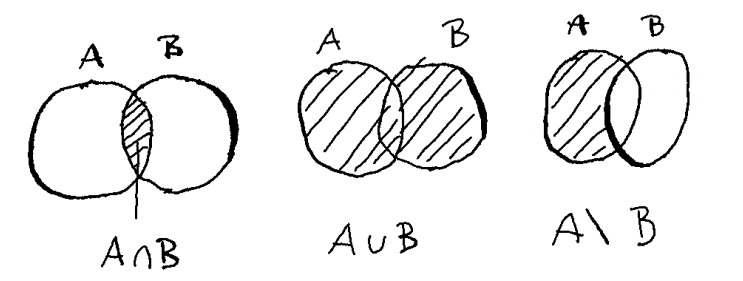
\includegraphics[width=0.5\textwidth]{img/mengenVenn.png}
    \caption{Venn Diagramme der Operationen auf Mengen $A$ und $B$.}
    \label{fig:vennMengen}
\end{figure}



\begin{figure}[h]
    \centering
    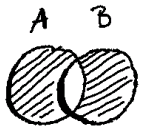
\includegraphics[width=0.1\textwidth]{img/mengen_symDiff.png}
    \caption{Symmetrische Differenz der Mengen $A$ und $B$.}
    \label{fig:venn_symDiff}
\end{figure}

\begin{question}
    Konstruiere die Situation in Abbildung \ref{fig:venn_symDiff}.
\end{question}

\begin{answer}
      $(A \cup B) \setminus (A \cap B)$. Siehe Abbildung \ref{fig:symDifSteps}.
\end{answer}

      \begin{figure}[h]
          \centering
          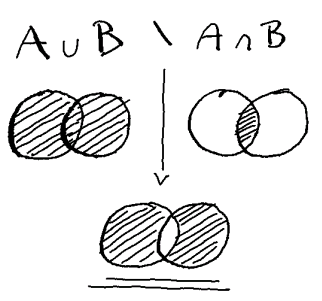
\includegraphics[width=0.2\textwidth]{img/symDifSteps.png}
          \caption{\emph{Symmetrische Differenz} in einzelnen Schritten veranschaulicht.}
          \label{fig:symDifSteps}
      \end{figure}


\subsection{Beschreibung von Teilmengen}
\begin{itemize}
    \item $A\subseteq B$. $A$ ist eine \textbf{Teilmenge} von $B$. Das heißt: $x \in A \implies x \in B$.
    \item $A\subset B$. $A$ ist eine \textbf{Echte Teilmenge} von $B$. Das heißt: $A\subseteq B \land A \neq B $.
\end{itemize}


\section{Funktionen, Abbildungen}
\label{sec:funktionen}

\todo[]{alles.}
Die \emph{Abbildung} oder \emph{Funktion} $f$ bildet die Menge $D$ auf die Menge $Z$ ab. Sie ordnet jedem Element von $D$ \emph{genau ein} Element von $Z$ zu.

    $$ f : D \to Z$$

Man schreibt $f\coloneqq x \mapsto y$ oder $f(x) = y$.

\begin{itemize}
    \item $D$ Definitionsbereich, Definitionsmenge
    \item $Z$ Zielmenge
    \item $f(A)$ Bildmenge (wobei stets $f(A)=B, B \in Z$, heißt: Die Bildmenge ist eine Teilmenge der Zielmenge.)
    \item $x$ unabhängige Variable
    \item $y$ abhängige Variable
    \item $f(x) = y$ Funktionsgleichung
\end{itemize}


\example{
    \textbf{Beispiel} \\
    $$f : \mathbb{R} \to \mathbb{R} , \: f(x) = sin(x)$$

    \begin{figure}[H]
        \centering
        %% Creator: Matplotlib, PGF backend
%%
%% To include the figure in your LaTeX document, write
%%   \input{<filename>.pgf}
%%
%% Make sure the required packages are loaded in your preamble
%%   \usepackage{pgf}
%%
%% Also ensure that all the required font packages are loaded; for instance,
%% the lmodern package is sometimes necessary when using math font.
%%   \usepackage{lmodern}
%%
%% Figures using additional raster images can only be included by \input if
%% they are in the same directory as the main LaTeX file. For loading figures
%% from other directories you can use the `import` package
%%   \usepackage{import}
%%
%% and then include the figures with
%%   \import{<path to file>}{<filename>.pgf}
%%
%% Matplotlib used the following preamble
%%   \def\mathdefault#1{#1}
%%   \everymath=\expandafter{\the\everymath\displaystyle}
%%   
%%   \usepackage{fontspec}
%%   \setmainfont{VeraSe.ttf}[Path=\detokenize{/usr/share/fonts/TTF/}]
%%   \setsansfont{DejaVuSans.ttf}[Path=\detokenize{/home/pl/miniconda3/lib/python3.12/site-packages/matplotlib/mpl-data/fonts/ttf/}]
%%   \setmonofont{DejaVuSansMono.ttf}[Path=\detokenize{/home/pl/miniconda3/lib/python3.12/site-packages/matplotlib/mpl-data/fonts/ttf/}]
%%   \makeatletter\@ifpackageloaded{underscore}{}{\usepackage[strings]{underscore}}\makeatother
%%
\begingroup%
\makeatletter%
\begin{pgfpicture}%
\pgfpathrectangle{\pgfpointorigin}{\pgfqpoint{2.956614in}{2.188486in}}%
\pgfusepath{use as bounding box, clip}%
\begin{pgfscope}%
\pgfsetbuttcap%
\pgfsetmiterjoin%
\definecolor{currentfill}{rgb}{1.000000,1.000000,1.000000}%
\pgfsetfillcolor{currentfill}%
\pgfsetlinewidth{0.000000pt}%
\definecolor{currentstroke}{rgb}{1.000000,1.000000,1.000000}%
\pgfsetstrokecolor{currentstroke}%
\pgfsetdash{}{0pt}%
\pgfpathmoveto{\pgfqpoint{0.000000in}{0.000000in}}%
\pgfpathlineto{\pgfqpoint{2.956614in}{0.000000in}}%
\pgfpathlineto{\pgfqpoint{2.956614in}{2.188486in}}%
\pgfpathlineto{\pgfqpoint{0.000000in}{2.188486in}}%
\pgfpathlineto{\pgfqpoint{0.000000in}{0.000000in}}%
\pgfpathclose%
\pgfusepath{fill}%
\end{pgfscope}%
\begin{pgfscope}%
\pgfsetbuttcap%
\pgfsetmiterjoin%
\definecolor{currentfill}{rgb}{1.000000,1.000000,1.000000}%
\pgfsetfillcolor{currentfill}%
\pgfsetlinewidth{0.000000pt}%
\definecolor{currentstroke}{rgb}{0.000000,0.000000,0.000000}%
\pgfsetstrokecolor{currentstroke}%
\pgfsetstrokeopacity{0.000000}%
\pgfsetdash{}{0pt}%
\pgfpathmoveto{\pgfqpoint{0.742978in}{0.548486in}}%
\pgfpathlineto{\pgfqpoint{2.856614in}{0.548486in}}%
\pgfpathlineto{\pgfqpoint{2.856614in}{2.088486in}}%
\pgfpathlineto{\pgfqpoint{0.742978in}{2.088486in}}%
\pgfpathlineto{\pgfqpoint{0.742978in}{0.548486in}}%
\pgfpathclose%
\pgfusepath{fill}%
\end{pgfscope}%
\begin{pgfscope}%
\pgfsetbuttcap%
\pgfsetroundjoin%
\definecolor{currentfill}{rgb}{0.000000,0.000000,0.000000}%
\pgfsetfillcolor{currentfill}%
\pgfsetlinewidth{0.803000pt}%
\definecolor{currentstroke}{rgb}{0.000000,0.000000,0.000000}%
\pgfsetstrokecolor{currentstroke}%
\pgfsetdash{}{0pt}%
\pgfsys@defobject{currentmarker}{\pgfqpoint{0.000000in}{-0.048611in}}{\pgfqpoint{0.000000in}{0.000000in}}{%
\pgfpathmoveto{\pgfqpoint{0.000000in}{0.000000in}}%
\pgfpathlineto{\pgfqpoint{0.000000in}{-0.048611in}}%
\pgfusepath{stroke,fill}%
}%
\begin{pgfscope}%
\pgfsys@transformshift{1.035260in}{0.548486in}%
\pgfsys@useobject{currentmarker}{}%
\end{pgfscope}%
\end{pgfscope}%
\begin{pgfscope}%
\definecolor{textcolor}{rgb}{0.000000,0.000000,0.000000}%
\pgfsetstrokecolor{textcolor}%
\pgfsetfillcolor{textcolor}%
\pgftext[x=1.035260in,y=0.451264in,,top]{\color{textcolor}{\rmfamily\fontsize{10.000000}{12.000000}\selectfont\catcode`\^=\active\def^{\ifmmode\sp\else\^{}\fi}\catcode`\%=\active\def%{\%}\ensuremath{-}5}}%
\end{pgfscope}%
\begin{pgfscope}%
\pgfsetbuttcap%
\pgfsetroundjoin%
\definecolor{currentfill}{rgb}{0.000000,0.000000,0.000000}%
\pgfsetfillcolor{currentfill}%
\pgfsetlinewidth{0.803000pt}%
\definecolor{currentstroke}{rgb}{0.000000,0.000000,0.000000}%
\pgfsetstrokecolor{currentstroke}%
\pgfsetdash{}{0pt}%
\pgfsys@defobject{currentmarker}{\pgfqpoint{0.000000in}{-0.048611in}}{\pgfqpoint{0.000000in}{0.000000in}}{%
\pgfpathmoveto{\pgfqpoint{0.000000in}{0.000000in}}%
\pgfpathlineto{\pgfqpoint{0.000000in}{-0.048611in}}%
\pgfusepath{stroke,fill}%
}%
\begin{pgfscope}%
\pgfsys@transformshift{1.799796in}{0.548486in}%
\pgfsys@useobject{currentmarker}{}%
\end{pgfscope}%
\end{pgfscope}%
\begin{pgfscope}%
\definecolor{textcolor}{rgb}{0.000000,0.000000,0.000000}%
\pgfsetstrokecolor{textcolor}%
\pgfsetfillcolor{textcolor}%
\pgftext[x=1.799796in,y=0.451264in,,top]{\color{textcolor}{\rmfamily\fontsize{10.000000}{12.000000}\selectfont\catcode`\^=\active\def^{\ifmmode\sp\else\^{}\fi}\catcode`\%=\active\def%{\%}0}}%
\end{pgfscope}%
\begin{pgfscope}%
\pgfsetbuttcap%
\pgfsetroundjoin%
\definecolor{currentfill}{rgb}{0.000000,0.000000,0.000000}%
\pgfsetfillcolor{currentfill}%
\pgfsetlinewidth{0.803000pt}%
\definecolor{currentstroke}{rgb}{0.000000,0.000000,0.000000}%
\pgfsetstrokecolor{currentstroke}%
\pgfsetdash{}{0pt}%
\pgfsys@defobject{currentmarker}{\pgfqpoint{0.000000in}{-0.048611in}}{\pgfqpoint{0.000000in}{0.000000in}}{%
\pgfpathmoveto{\pgfqpoint{0.000000in}{0.000000in}}%
\pgfpathlineto{\pgfqpoint{0.000000in}{-0.048611in}}%
\pgfusepath{stroke,fill}%
}%
\begin{pgfscope}%
\pgfsys@transformshift{2.564331in}{0.548486in}%
\pgfsys@useobject{currentmarker}{}%
\end{pgfscope}%
\end{pgfscope}%
\begin{pgfscope}%
\definecolor{textcolor}{rgb}{0.000000,0.000000,0.000000}%
\pgfsetstrokecolor{textcolor}%
\pgfsetfillcolor{textcolor}%
\pgftext[x=2.564331in,y=0.451264in,,top]{\color{textcolor}{\rmfamily\fontsize{10.000000}{12.000000}\selectfont\catcode`\^=\active\def^{\ifmmode\sp\else\^{}\fi}\catcode`\%=\active\def%{\%}5}}%
\end{pgfscope}%
\begin{pgfscope}%
\definecolor{textcolor}{rgb}{0.000000,0.000000,0.000000}%
\pgfsetstrokecolor{textcolor}%
\pgfsetfillcolor{textcolor}%
\pgftext[x=1.799796in,y=0.261295in,,top]{\color{textcolor}{\rmfamily\fontsize{12.000000}{14.400000}\selectfont\catcode`\^=\active\def^{\ifmmode\sp\else\^{}\fi}\catcode`\%=\active\def%{\%}$x$}}%
\end{pgfscope}%
\begin{pgfscope}%
\pgfsetbuttcap%
\pgfsetroundjoin%
\definecolor{currentfill}{rgb}{0.000000,0.000000,0.000000}%
\pgfsetfillcolor{currentfill}%
\pgfsetlinewidth{0.803000pt}%
\definecolor{currentstroke}{rgb}{0.000000,0.000000,0.000000}%
\pgfsetstrokecolor{currentstroke}%
\pgfsetdash{}{0pt}%
\pgfsys@defobject{currentmarker}{\pgfqpoint{-0.048611in}{0.000000in}}{\pgfqpoint{-0.000000in}{0.000000in}}{%
\pgfpathmoveto{\pgfqpoint{-0.000000in}{0.000000in}}%
\pgfpathlineto{\pgfqpoint{-0.048611in}{0.000000in}}%
\pgfusepath{stroke,fill}%
}%
\begin{pgfscope}%
\pgfsys@transformshift{0.742978in}{0.676819in}%
\pgfsys@useobject{currentmarker}{}%
\end{pgfscope}%
\end{pgfscope}%
\begin{pgfscope}%
\definecolor{textcolor}{rgb}{0.000000,0.000000,0.000000}%
\pgfsetstrokecolor{textcolor}%
\pgfsetfillcolor{textcolor}%
\pgftext[x=0.316851in, y=0.624058in, left, base]{\color{textcolor}{\rmfamily\fontsize{10.000000}{12.000000}\selectfont\catcode`\^=\active\def^{\ifmmode\sp\else\^{}\fi}\catcode`\%=\active\def%{\%}\ensuremath{-}1.0}}%
\end{pgfscope}%
\begin{pgfscope}%
\pgfsetbuttcap%
\pgfsetroundjoin%
\definecolor{currentfill}{rgb}{0.000000,0.000000,0.000000}%
\pgfsetfillcolor{currentfill}%
\pgfsetlinewidth{0.803000pt}%
\definecolor{currentstroke}{rgb}{0.000000,0.000000,0.000000}%
\pgfsetstrokecolor{currentstroke}%
\pgfsetdash{}{0pt}%
\pgfsys@defobject{currentmarker}{\pgfqpoint{-0.048611in}{0.000000in}}{\pgfqpoint{-0.000000in}{0.000000in}}{%
\pgfpathmoveto{\pgfqpoint{-0.000000in}{0.000000in}}%
\pgfpathlineto{\pgfqpoint{-0.048611in}{0.000000in}}%
\pgfusepath{stroke,fill}%
}%
\begin{pgfscope}%
\pgfsys@transformshift{0.742978in}{0.997653in}%
\pgfsys@useobject{currentmarker}{}%
\end{pgfscope}%
\end{pgfscope}%
\begin{pgfscope}%
\definecolor{textcolor}{rgb}{0.000000,0.000000,0.000000}%
\pgfsetstrokecolor{textcolor}%
\pgfsetfillcolor{textcolor}%
\pgftext[x=0.316851in, y=0.944891in, left, base]{\color{textcolor}{\rmfamily\fontsize{10.000000}{12.000000}\selectfont\catcode`\^=\active\def^{\ifmmode\sp\else\^{}\fi}\catcode`\%=\active\def%{\%}\ensuremath{-}0.5}}%
\end{pgfscope}%
\begin{pgfscope}%
\pgfsetbuttcap%
\pgfsetroundjoin%
\definecolor{currentfill}{rgb}{0.000000,0.000000,0.000000}%
\pgfsetfillcolor{currentfill}%
\pgfsetlinewidth{0.803000pt}%
\definecolor{currentstroke}{rgb}{0.000000,0.000000,0.000000}%
\pgfsetstrokecolor{currentstroke}%
\pgfsetdash{}{0pt}%
\pgfsys@defobject{currentmarker}{\pgfqpoint{-0.048611in}{0.000000in}}{\pgfqpoint{-0.000000in}{0.000000in}}{%
\pgfpathmoveto{\pgfqpoint{-0.000000in}{0.000000in}}%
\pgfpathlineto{\pgfqpoint{-0.048611in}{0.000000in}}%
\pgfusepath{stroke,fill}%
}%
\begin{pgfscope}%
\pgfsys@transformshift{0.742978in}{1.318486in}%
\pgfsys@useobject{currentmarker}{}%
\end{pgfscope}%
\end{pgfscope}%
\begin{pgfscope}%
\definecolor{textcolor}{rgb}{0.000000,0.000000,0.000000}%
\pgfsetstrokecolor{textcolor}%
\pgfsetfillcolor{textcolor}%
\pgftext[x=0.424876in, y=1.265724in, left, base]{\color{textcolor}{\rmfamily\fontsize{10.000000}{12.000000}\selectfont\catcode`\^=\active\def^{\ifmmode\sp\else\^{}\fi}\catcode`\%=\active\def%{\%}0.0}}%
\end{pgfscope}%
\begin{pgfscope}%
\pgfsetbuttcap%
\pgfsetroundjoin%
\definecolor{currentfill}{rgb}{0.000000,0.000000,0.000000}%
\pgfsetfillcolor{currentfill}%
\pgfsetlinewidth{0.803000pt}%
\definecolor{currentstroke}{rgb}{0.000000,0.000000,0.000000}%
\pgfsetstrokecolor{currentstroke}%
\pgfsetdash{}{0pt}%
\pgfsys@defobject{currentmarker}{\pgfqpoint{-0.048611in}{0.000000in}}{\pgfqpoint{-0.000000in}{0.000000in}}{%
\pgfpathmoveto{\pgfqpoint{-0.000000in}{0.000000in}}%
\pgfpathlineto{\pgfqpoint{-0.048611in}{0.000000in}}%
\pgfusepath{stroke,fill}%
}%
\begin{pgfscope}%
\pgfsys@transformshift{0.742978in}{1.639319in}%
\pgfsys@useobject{currentmarker}{}%
\end{pgfscope}%
\end{pgfscope}%
\begin{pgfscope}%
\definecolor{textcolor}{rgb}{0.000000,0.000000,0.000000}%
\pgfsetstrokecolor{textcolor}%
\pgfsetfillcolor{textcolor}%
\pgftext[x=0.424876in, y=1.586558in, left, base]{\color{textcolor}{\rmfamily\fontsize{10.000000}{12.000000}\selectfont\catcode`\^=\active\def^{\ifmmode\sp\else\^{}\fi}\catcode`\%=\active\def%{\%}0.5}}%
\end{pgfscope}%
\begin{pgfscope}%
\pgfsetbuttcap%
\pgfsetroundjoin%
\definecolor{currentfill}{rgb}{0.000000,0.000000,0.000000}%
\pgfsetfillcolor{currentfill}%
\pgfsetlinewidth{0.803000pt}%
\definecolor{currentstroke}{rgb}{0.000000,0.000000,0.000000}%
\pgfsetstrokecolor{currentstroke}%
\pgfsetdash{}{0pt}%
\pgfsys@defobject{currentmarker}{\pgfqpoint{-0.048611in}{0.000000in}}{\pgfqpoint{-0.000000in}{0.000000in}}{%
\pgfpathmoveto{\pgfqpoint{-0.000000in}{0.000000in}}%
\pgfpathlineto{\pgfqpoint{-0.048611in}{0.000000in}}%
\pgfusepath{stroke,fill}%
}%
\begin{pgfscope}%
\pgfsys@transformshift{0.742978in}{1.960153in}%
\pgfsys@useobject{currentmarker}{}%
\end{pgfscope}%
\end{pgfscope}%
\begin{pgfscope}%
\definecolor{textcolor}{rgb}{0.000000,0.000000,0.000000}%
\pgfsetstrokecolor{textcolor}%
\pgfsetfillcolor{textcolor}%
\pgftext[x=0.424876in, y=1.907391in, left, base]{\color{textcolor}{\rmfamily\fontsize{10.000000}{12.000000}\selectfont\catcode`\^=\active\def^{\ifmmode\sp\else\^{}\fi}\catcode`\%=\active\def%{\%}1.0}}%
\end{pgfscope}%
\begin{pgfscope}%
\definecolor{textcolor}{rgb}{0.000000,0.000000,0.000000}%
\pgfsetstrokecolor{textcolor}%
\pgfsetfillcolor{textcolor}%
\pgftext[x=0.261295in,y=1.318486in,,bottom,rotate=90.000000]{\color{textcolor}{\rmfamily\fontsize{12.000000}{14.400000}\selectfont\catcode`\^=\active\def^{\ifmmode\sp\else\^{}\fi}\catcode`\%=\active\def%{\%}$y$}}%
\end{pgfscope}%
\begin{pgfscope}%
\pgfpathrectangle{\pgfqpoint{0.742978in}{0.548486in}}{\pgfqpoint{2.113636in}{1.540000in}}%
\pgfusepath{clip}%
\pgfsetrectcap%
\pgfsetroundjoin%
\pgfsetlinewidth{1.505625pt}%
\definecolor{currentstroke}{rgb}{0.000000,0.000000,0.000000}%
\pgfsetstrokecolor{currentstroke}%
\pgfsetdash{}{0pt}%
\pgfpathmoveto{\pgfqpoint{0.839052in}{1.318486in}}%
\pgfpathlineto{\pgfqpoint{0.858461in}{1.399716in}}%
\pgfpathlineto{\pgfqpoint{0.877870in}{1.479639in}}%
\pgfpathlineto{\pgfqpoint{0.897279in}{1.556969in}}%
\pgfpathlineto{\pgfqpoint{0.916688in}{1.630462in}}%
\pgfpathlineto{\pgfqpoint{0.936097in}{1.698935in}}%
\pgfpathlineto{\pgfqpoint{0.955506in}{1.761287in}}%
\pgfpathlineto{\pgfqpoint{0.974915in}{1.816513in}}%
\pgfpathlineto{\pgfqpoint{0.994324in}{1.863726in}}%
\pgfpathlineto{\pgfqpoint{1.013733in}{1.902167in}}%
\pgfpathlineto{\pgfqpoint{1.033142in}{1.931215in}}%
\pgfpathlineto{\pgfqpoint{1.052551in}{1.950404in}}%
\pgfpathlineto{\pgfqpoint{1.071960in}{1.959426in}}%
\pgfpathlineto{\pgfqpoint{1.091369in}{1.958134in}}%
\pgfpathlineto{\pgfqpoint{1.110778in}{1.946551in}}%
\pgfpathlineto{\pgfqpoint{1.130187in}{1.924861in}}%
\pgfpathlineto{\pgfqpoint{1.149595in}{1.893415in}}%
\pgfpathlineto{\pgfqpoint{1.169004in}{1.852718in}}%
\pgfpathlineto{\pgfqpoint{1.188413in}{1.803425in}}%
\pgfpathlineto{\pgfqpoint{1.207822in}{1.746329in}}%
\pgfpathlineto{\pgfqpoint{1.227231in}{1.682349in}}%
\pgfpathlineto{\pgfqpoint{1.246640in}{1.612515in}}%
\pgfpathlineto{\pgfqpoint{1.266049in}{1.537949in}}%
\pgfpathlineto{\pgfqpoint{1.285458in}{1.459852in}}%
\pgfpathlineto{\pgfqpoint{1.304867in}{1.379480in}}%
\pgfpathlineto{\pgfqpoint{1.324276in}{1.298127in}}%
\pgfpathlineto{\pgfqpoint{1.343685in}{1.217102in}}%
\pgfpathlineto{\pgfqpoint{1.363094in}{1.137708in}}%
\pgfpathlineto{\pgfqpoint{1.382503in}{1.061222in}}%
\pgfpathlineto{\pgfqpoint{1.401912in}{0.988876in}}%
\pgfpathlineto{\pgfqpoint{1.421321in}{0.921834in}}%
\pgfpathlineto{\pgfqpoint{1.440730in}{0.861174in}}%
\pgfpathlineto{\pgfqpoint{1.460139in}{0.807872in}}%
\pgfpathlineto{\pgfqpoint{1.479548in}{0.762786in}}%
\pgfpathlineto{\pgfqpoint{1.498957in}{0.726642in}}%
\pgfpathlineto{\pgfqpoint{1.518366in}{0.700021in}}%
\pgfpathlineto{\pgfqpoint{1.537775in}{0.683351in}}%
\pgfpathlineto{\pgfqpoint{1.557184in}{0.676900in}}%
\pgfpathlineto{\pgfqpoint{1.576593in}{0.680773in}}%
\pgfpathlineto{\pgfqpoint{1.596002in}{0.694907in}}%
\pgfpathlineto{\pgfqpoint{1.615411in}{0.719074in}}%
\pgfpathlineto{\pgfqpoint{1.634820in}{0.752887in}}%
\pgfpathlineto{\pgfqpoint{1.654229in}{0.795800in}}%
\pgfpathlineto{\pgfqpoint{1.673638in}{0.847123in}}%
\pgfpathlineto{\pgfqpoint{1.693047in}{0.906031in}}%
\pgfpathlineto{\pgfqpoint{1.712455in}{0.971575in}}%
\pgfpathlineto{\pgfqpoint{1.731864in}{1.042701in}}%
\pgfpathlineto{\pgfqpoint{1.751273in}{1.118265in}}%
\pgfpathlineto{\pgfqpoint{1.770682in}{1.197050in}}%
\pgfpathlineto{\pgfqpoint{1.790091in}{1.277789in}}%
\pgfpathlineto{\pgfqpoint{1.809500in}{1.359183in}}%
\pgfpathlineto{\pgfqpoint{1.828909in}{1.439922in}}%
\pgfpathlineto{\pgfqpoint{1.848318in}{1.518707in}}%
\pgfpathlineto{\pgfqpoint{1.867727in}{1.594271in}}%
\pgfpathlineto{\pgfqpoint{1.887136in}{1.665397in}}%
\pgfpathlineto{\pgfqpoint{1.906545in}{1.730941in}}%
\pgfpathlineto{\pgfqpoint{1.925954in}{1.789849in}}%
\pgfpathlineto{\pgfqpoint{1.945363in}{1.841172in}}%
\pgfpathlineto{\pgfqpoint{1.964772in}{1.884085in}}%
\pgfpathlineto{\pgfqpoint{1.984181in}{1.917898in}}%
\pgfpathlineto{\pgfqpoint{2.003590in}{1.942065in}}%
\pgfpathlineto{\pgfqpoint{2.022999in}{1.956199in}}%
\pgfpathlineto{\pgfqpoint{2.042408in}{1.960072in}}%
\pgfpathlineto{\pgfqpoint{2.061817in}{1.953621in}}%
\pgfpathlineto{\pgfqpoint{2.081226in}{1.936951in}}%
\pgfpathlineto{\pgfqpoint{2.100635in}{1.910330in}}%
\pgfpathlineto{\pgfqpoint{2.120044in}{1.874186in}}%
\pgfpathlineto{\pgfqpoint{2.139453in}{1.829100in}}%
\pgfpathlineto{\pgfqpoint{2.158862in}{1.775798in}}%
\pgfpathlineto{\pgfqpoint{2.178271in}{1.715138in}}%
\pgfpathlineto{\pgfqpoint{2.197680in}{1.648096in}}%
\pgfpathlineto{\pgfqpoint{2.217089in}{1.575750in}}%
\pgfpathlineto{\pgfqpoint{2.236498in}{1.499264in}}%
\pgfpathlineto{\pgfqpoint{2.255907in}{1.419870in}}%
\pgfpathlineto{\pgfqpoint{2.275315in}{1.338845in}}%
\pgfpathlineto{\pgfqpoint{2.294724in}{1.257492in}}%
\pgfpathlineto{\pgfqpoint{2.314133in}{1.177120in}}%
\pgfpathlineto{\pgfqpoint{2.333542in}{1.099023in}}%
\pgfpathlineto{\pgfqpoint{2.352951in}{1.024457in}}%
\pgfpathlineto{\pgfqpoint{2.372360in}{0.954623in}}%
\pgfpathlineto{\pgfqpoint{2.391769in}{0.890643in}}%
\pgfpathlineto{\pgfqpoint{2.411178in}{0.833547in}}%
\pgfpathlineto{\pgfqpoint{2.430587in}{0.784254in}}%
\pgfpathlineto{\pgfqpoint{2.449996in}{0.743557in}}%
\pgfpathlineto{\pgfqpoint{2.469405in}{0.712110in}}%
\pgfpathlineto{\pgfqpoint{2.488814in}{0.690421in}}%
\pgfpathlineto{\pgfqpoint{2.508223in}{0.678837in}}%
\pgfpathlineto{\pgfqpoint{2.527632in}{0.677546in}}%
\pgfpathlineto{\pgfqpoint{2.547041in}{0.686568in}}%
\pgfpathlineto{\pgfqpoint{2.566450in}{0.705757in}}%
\pgfpathlineto{\pgfqpoint{2.585859in}{0.734805in}}%
\pgfpathlineto{\pgfqpoint{2.605268in}{0.773245in}}%
\pgfpathlineto{\pgfqpoint{2.624677in}{0.820459in}}%
\pgfpathlineto{\pgfqpoint{2.644086in}{0.875685in}}%
\pgfpathlineto{\pgfqpoint{2.663495in}{0.938037in}}%
\pgfpathlineto{\pgfqpoint{2.682904in}{1.006510in}}%
\pgfpathlineto{\pgfqpoint{2.702313in}{1.080003in}}%
\pgfpathlineto{\pgfqpoint{2.721722in}{1.157333in}}%
\pgfpathlineto{\pgfqpoint{2.741131in}{1.237256in}}%
\pgfpathlineto{\pgfqpoint{2.760540in}{1.318486in}}%
\pgfusepath{stroke}%
\end{pgfscope}%
\begin{pgfscope}%
\pgfpathrectangle{\pgfqpoint{0.742978in}{0.548486in}}{\pgfqpoint{2.113636in}{1.540000in}}%
\pgfusepath{clip}%
\pgfsetrectcap%
\pgfsetroundjoin%
\pgfsetlinewidth{0.501875pt}%
\definecolor{currentstroke}{rgb}{0.000000,0.000000,0.000000}%
\pgfsetstrokecolor{currentstroke}%
\pgfsetdash{}{0pt}%
\pgfpathmoveto{\pgfqpoint{0.742978in}{1.318486in}}%
\pgfpathlineto{\pgfqpoint{2.856614in}{1.318486in}}%
\pgfusepath{stroke}%
\end{pgfscope}%
\begin{pgfscope}%
\pgfpathrectangle{\pgfqpoint{0.742978in}{0.548486in}}{\pgfqpoint{2.113636in}{1.540000in}}%
\pgfusepath{clip}%
\pgfsetrectcap%
\pgfsetroundjoin%
\pgfsetlinewidth{0.501875pt}%
\definecolor{currentstroke}{rgb}{0.000000,0.000000,0.000000}%
\pgfsetstrokecolor{currentstroke}%
\pgfsetdash{}{0pt}%
\pgfpathmoveto{\pgfqpoint{1.799796in}{0.548486in}}%
\pgfpathlineto{\pgfqpoint{1.799796in}{2.088486in}}%
\pgfusepath{stroke}%
\end{pgfscope}%
\begin{pgfscope}%
\pgfsetbuttcap%
\pgfsetmiterjoin%
\definecolor{currentfill}{rgb}{1.000000,1.000000,1.000000}%
\pgfsetfillcolor{currentfill}%
\pgfsetfillopacity{0.800000}%
\pgfsetlinewidth{1.003750pt}%
\definecolor{currentstroke}{rgb}{0.800000,0.800000,0.800000}%
\pgfsetstrokecolor{currentstroke}%
\pgfsetstrokeopacity{0.800000}%
\pgfsetdash{}{0pt}%
\pgfpathmoveto{\pgfqpoint{2.044596in}{1.767685in}}%
\pgfpathlineto{\pgfqpoint{2.759392in}{1.767685in}}%
\pgfpathquadraticcurveto{\pgfqpoint{2.787170in}{1.767685in}}{\pgfqpoint{2.787170in}{1.795463in}}%
\pgfpathlineto{\pgfqpoint{2.787170in}{1.991264in}}%
\pgfpathquadraticcurveto{\pgfqpoint{2.787170in}{2.019042in}}{\pgfqpoint{2.759392in}{2.019042in}}%
\pgfpathlineto{\pgfqpoint{2.044596in}{2.019042in}}%
\pgfpathquadraticcurveto{\pgfqpoint{2.016818in}{2.019042in}}{\pgfqpoint{2.016818in}{1.991264in}}%
\pgfpathlineto{\pgfqpoint{2.016818in}{1.795463in}}%
\pgfpathquadraticcurveto{\pgfqpoint{2.016818in}{1.767685in}}{\pgfqpoint{2.044596in}{1.767685in}}%
\pgfpathlineto{\pgfqpoint{2.044596in}{1.767685in}}%
\pgfpathclose%
\pgfusepath{stroke,fill}%
\end{pgfscope}%
\begin{pgfscope}%
\pgfsetrectcap%
\pgfsetroundjoin%
\pgfsetlinewidth{1.505625pt}%
\definecolor{currentstroke}{rgb}{0.000000,0.000000,0.000000}%
\pgfsetstrokecolor{currentstroke}%
\pgfsetdash{}{0pt}%
\pgfpathmoveto{\pgfqpoint{2.072373in}{1.906574in}}%
\pgfpathlineto{\pgfqpoint{2.211262in}{1.906574in}}%
\pgfpathlineto{\pgfqpoint{2.350151in}{1.906574in}}%
\pgfusepath{stroke}%
\end{pgfscope}%
\begin{pgfscope}%
\definecolor{textcolor}{rgb}{0.000000,0.000000,0.000000}%
\pgfsetstrokecolor{textcolor}%
\pgfsetfillcolor{textcolor}%
\pgftext[x=2.461262in,y=1.857963in,left,base]{\color{textcolor}{\rmfamily\fontsize{10.000000}{12.000000}\selectfont\catcode`\^=\active\def^{\ifmmode\sp\else\^{}\fi}\catcode`\%=\active\def%{\%}$f(x)$}}%
\end{pgfscope}%
\end{pgfpicture}%
\makeatother%
\endgroup%

        % \includegraphics[]{}
        \caption{Der Funktionsgraph der Funktion $f(x)$.}
        \label{fig:figure1}
    \end{figure}
}

\subsection{Gerade und Ungerade Funktionen}\label{subsec:geradeUngerade}
Von \href{https://de.wikipedia.org/wiki/Gerade\_und\_ungerade\_Funktionen}{Wikipedia}, um zu demonstrieren dass das zuvor gelernte ständig anzutreffen ist:

\emph{'Eine reelle Funktion $f\colon D\to \mathbb {R} $ mit einer bezüglich der Null symmetrischen Definitionsmenge 
$ D\subseteq \mathbb {R}$ heißt gerade, wenn für alle Argumente $ x\in D$  $f(-x)=f(x)$.'} \\

Ungerade und Gerade Funktionen kurz zusammengefasst:
\begin{itemize}
    \item Gerade Funktion:  $f(-x) = f(x)$. Achsensymmetrisch zur $y$-Achse.
    \item Ungerade Funktion:  $f(-x) = -f(x)$. Punktsymmetrisch zum Ursprung.
\end{itemize}

    \begin{figure}[H]
        \centering
        %% Creator: Matplotlib, PGF backend
%%
%% To include the figure in your LaTeX document, write
%%   \input{<filename>.pgf}
%%
%% Make sure the required packages are loaded in your preamble
%%   \usepackage{pgf}
%%
%% Also ensure that all the required font packages are loaded; for instance,
%% the lmodern package is sometimes necessary when using math font.
%%   \usepackage{lmodern}
%%
%% Figures using additional raster images can only be included by \input if
%% they are in the same directory as the main LaTeX file. For loading figures
%% from other directories you can use the `import` package
%%   \usepackage{import}
%%
%% and then include the figures with
%%   \import{<path to file>}{<filename>.pgf}
%%
%% Matplotlib used the following preamble
%%   
%%   \usepackage{fontspec}
%%   \setmainfont{DejaVuSerif.ttf}[Path=\detokenize{/home/pl/anaconda3/lib/python3.11/site-packages/matplotlib/mpl-data/fonts/ttf/}]
%%   \setsansfont{DejaVuSans.ttf}[Path=\detokenize{/home/pl/anaconda3/lib/python3.11/site-packages/matplotlib/mpl-data/fonts/ttf/}]
%%   \setmonofont{DejaVuSansMono.ttf}[Path=\detokenize{/home/pl/anaconda3/lib/python3.11/site-packages/matplotlib/mpl-data/fonts/ttf/}]
%%   \makeatletter\@ifpackageloaded{underscore}{}{\usepackage[strings]{underscore}}\makeatother
%%
\begingroup%
\makeatletter%
\begin{pgfpicture}%
\pgfpathrectangle{\pgfpointorigin}{\pgfqpoint{5.347946in}{2.984365in}}%
\pgfusepath{use as bounding box, clip}%
\begin{pgfscope}%
\pgfsetbuttcap%
\pgfsetmiterjoin%
\definecolor{currentfill}{rgb}{1.000000,1.000000,1.000000}%
\pgfsetfillcolor{currentfill}%
\pgfsetlinewidth{0.000000pt}%
\definecolor{currentstroke}{rgb}{1.000000,1.000000,1.000000}%
\pgfsetstrokecolor{currentstroke}%
\pgfsetdash{}{0pt}%
\pgfpathmoveto{\pgfqpoint{0.000000in}{0.000000in}}%
\pgfpathlineto{\pgfqpoint{5.347946in}{0.000000in}}%
\pgfpathlineto{\pgfqpoint{5.347946in}{2.984365in}}%
\pgfpathlineto{\pgfqpoint{0.000000in}{2.984365in}}%
\pgfpathlineto{\pgfqpoint{0.000000in}{0.000000in}}%
\pgfpathclose%
\pgfusepath{fill}%
\end{pgfscope}%
\begin{pgfscope}%
\pgfsetbuttcap%
\pgfsetmiterjoin%
\definecolor{currentfill}{rgb}{1.000000,1.000000,1.000000}%
\pgfsetfillcolor{currentfill}%
\pgfsetlinewidth{0.000000pt}%
\definecolor{currentstroke}{rgb}{0.000000,0.000000,0.000000}%
\pgfsetstrokecolor{currentstroke}%
\pgfsetstrokeopacity{0.000000}%
\pgfsetdash{}{0pt}%
\pgfpathmoveto{\pgfqpoint{0.583581in}{0.521603in}}%
\pgfpathlineto{\pgfqpoint{2.697217in}{0.521603in}}%
\pgfpathlineto{\pgfqpoint{2.697217in}{2.831603in}}%
\pgfpathlineto{\pgfqpoint{0.583581in}{2.831603in}}%
\pgfpathlineto{\pgfqpoint{0.583581in}{0.521603in}}%
\pgfpathclose%
\pgfusepath{fill}%
\end{pgfscope}%
\begin{pgfscope}%
\pgfsetbuttcap%
\pgfsetroundjoin%
\definecolor{currentfill}{rgb}{0.000000,0.000000,0.000000}%
\pgfsetfillcolor{currentfill}%
\pgfsetlinewidth{0.803000pt}%
\definecolor{currentstroke}{rgb}{0.000000,0.000000,0.000000}%
\pgfsetstrokecolor{currentstroke}%
\pgfsetdash{}{0pt}%
\pgfsys@defobject{currentmarker}{\pgfqpoint{0.000000in}{-0.048611in}}{\pgfqpoint{0.000000in}{0.000000in}}{%
\pgfpathmoveto{\pgfqpoint{0.000000in}{0.000000in}}%
\pgfpathlineto{\pgfqpoint{0.000000in}{-0.048611in}}%
\pgfusepath{stroke,fill}%
}%
\begin{pgfscope}%
\pgfsys@transformshift{0.679655in}{0.521603in}%
\pgfsys@useobject{currentmarker}{}%
\end{pgfscope}%
\end{pgfscope}%
\begin{pgfscope}%
\definecolor{textcolor}{rgb}{0.000000,0.000000,0.000000}%
\pgfsetstrokecolor{textcolor}%
\pgfsetfillcolor{textcolor}%
\pgftext[x=0.679655in,y=0.424381in,,top]{\color{textcolor}\rmfamily\fontsize{10.000000}{12.000000}\selectfont \ensuremath{-}5.0}%
\end{pgfscope}%
\begin{pgfscope}%
\pgfsetbuttcap%
\pgfsetroundjoin%
\definecolor{currentfill}{rgb}{0.000000,0.000000,0.000000}%
\pgfsetfillcolor{currentfill}%
\pgfsetlinewidth{0.803000pt}%
\definecolor{currentstroke}{rgb}{0.000000,0.000000,0.000000}%
\pgfsetstrokecolor{currentstroke}%
\pgfsetdash{}{0pt}%
\pgfsys@defobject{currentmarker}{\pgfqpoint{0.000000in}{-0.048611in}}{\pgfqpoint{0.000000in}{0.000000in}}{%
\pgfpathmoveto{\pgfqpoint{0.000000in}{0.000000in}}%
\pgfpathlineto{\pgfqpoint{0.000000in}{-0.048611in}}%
\pgfusepath{stroke,fill}%
}%
\begin{pgfscope}%
\pgfsys@transformshift{1.160027in}{0.521603in}%
\pgfsys@useobject{currentmarker}{}%
\end{pgfscope}%
\end{pgfscope}%
\begin{pgfscope}%
\definecolor{textcolor}{rgb}{0.000000,0.000000,0.000000}%
\pgfsetstrokecolor{textcolor}%
\pgfsetfillcolor{textcolor}%
\pgftext[x=1.160027in,y=0.424381in,,top]{\color{textcolor}\rmfamily\fontsize{10.000000}{12.000000}\selectfont \ensuremath{-}2.5}%
\end{pgfscope}%
\begin{pgfscope}%
\pgfsetbuttcap%
\pgfsetroundjoin%
\definecolor{currentfill}{rgb}{0.000000,0.000000,0.000000}%
\pgfsetfillcolor{currentfill}%
\pgfsetlinewidth{0.803000pt}%
\definecolor{currentstroke}{rgb}{0.000000,0.000000,0.000000}%
\pgfsetstrokecolor{currentstroke}%
\pgfsetdash{}{0pt}%
\pgfsys@defobject{currentmarker}{\pgfqpoint{0.000000in}{-0.048611in}}{\pgfqpoint{0.000000in}{0.000000in}}{%
\pgfpathmoveto{\pgfqpoint{0.000000in}{0.000000in}}%
\pgfpathlineto{\pgfqpoint{0.000000in}{-0.048611in}}%
\pgfusepath{stroke,fill}%
}%
\begin{pgfscope}%
\pgfsys@transformshift{1.640399in}{0.521603in}%
\pgfsys@useobject{currentmarker}{}%
\end{pgfscope}%
\end{pgfscope}%
\begin{pgfscope}%
\definecolor{textcolor}{rgb}{0.000000,0.000000,0.000000}%
\pgfsetstrokecolor{textcolor}%
\pgfsetfillcolor{textcolor}%
\pgftext[x=1.640399in,y=0.424381in,,top]{\color{textcolor}\rmfamily\fontsize{10.000000}{12.000000}\selectfont 0.0}%
\end{pgfscope}%
\begin{pgfscope}%
\pgfsetbuttcap%
\pgfsetroundjoin%
\definecolor{currentfill}{rgb}{0.000000,0.000000,0.000000}%
\pgfsetfillcolor{currentfill}%
\pgfsetlinewidth{0.803000pt}%
\definecolor{currentstroke}{rgb}{0.000000,0.000000,0.000000}%
\pgfsetstrokecolor{currentstroke}%
\pgfsetdash{}{0pt}%
\pgfsys@defobject{currentmarker}{\pgfqpoint{0.000000in}{-0.048611in}}{\pgfqpoint{0.000000in}{0.000000in}}{%
\pgfpathmoveto{\pgfqpoint{0.000000in}{0.000000in}}%
\pgfpathlineto{\pgfqpoint{0.000000in}{-0.048611in}}%
\pgfusepath{stroke,fill}%
}%
\begin{pgfscope}%
\pgfsys@transformshift{2.120771in}{0.521603in}%
\pgfsys@useobject{currentmarker}{}%
\end{pgfscope}%
\end{pgfscope}%
\begin{pgfscope}%
\definecolor{textcolor}{rgb}{0.000000,0.000000,0.000000}%
\pgfsetstrokecolor{textcolor}%
\pgfsetfillcolor{textcolor}%
\pgftext[x=2.120771in,y=0.424381in,,top]{\color{textcolor}\rmfamily\fontsize{10.000000}{12.000000}\selectfont 2.5}%
\end{pgfscope}%
\begin{pgfscope}%
\pgfsetbuttcap%
\pgfsetroundjoin%
\definecolor{currentfill}{rgb}{0.000000,0.000000,0.000000}%
\pgfsetfillcolor{currentfill}%
\pgfsetlinewidth{0.803000pt}%
\definecolor{currentstroke}{rgb}{0.000000,0.000000,0.000000}%
\pgfsetstrokecolor{currentstroke}%
\pgfsetdash{}{0pt}%
\pgfsys@defobject{currentmarker}{\pgfqpoint{0.000000in}{-0.048611in}}{\pgfqpoint{0.000000in}{0.000000in}}{%
\pgfpathmoveto{\pgfqpoint{0.000000in}{0.000000in}}%
\pgfpathlineto{\pgfqpoint{0.000000in}{-0.048611in}}%
\pgfusepath{stroke,fill}%
}%
\begin{pgfscope}%
\pgfsys@transformshift{2.601143in}{0.521603in}%
\pgfsys@useobject{currentmarker}{}%
\end{pgfscope}%
\end{pgfscope}%
\begin{pgfscope}%
\definecolor{textcolor}{rgb}{0.000000,0.000000,0.000000}%
\pgfsetstrokecolor{textcolor}%
\pgfsetfillcolor{textcolor}%
\pgftext[x=2.601143in,y=0.424381in,,top]{\color{textcolor}\rmfamily\fontsize{10.000000}{12.000000}\selectfont 5.0}%
\end{pgfscope}%
\begin{pgfscope}%
\definecolor{textcolor}{rgb}{0.000000,0.000000,0.000000}%
\pgfsetstrokecolor{textcolor}%
\pgfsetfillcolor{textcolor}%
\pgftext[x=1.640399in,y=0.234413in,,top]{\color{textcolor}\rmfamily\fontsize{10.000000}{12.000000}\selectfont \(\displaystyle x\)}%
\end{pgfscope}%
\begin{pgfscope}%
\pgfsetbuttcap%
\pgfsetroundjoin%
\definecolor{currentfill}{rgb}{0.000000,0.000000,0.000000}%
\pgfsetfillcolor{currentfill}%
\pgfsetlinewidth{0.803000pt}%
\definecolor{currentstroke}{rgb}{0.000000,0.000000,0.000000}%
\pgfsetstrokecolor{currentstroke}%
\pgfsetdash{}{0pt}%
\pgfsys@defobject{currentmarker}{\pgfqpoint{-0.048611in}{0.000000in}}{\pgfqpoint{-0.000000in}{0.000000in}}{%
\pgfpathmoveto{\pgfqpoint{-0.000000in}{0.000000in}}%
\pgfpathlineto{\pgfqpoint{-0.048611in}{0.000000in}}%
\pgfusepath{stroke,fill}%
}%
\begin{pgfscope}%
\pgfsys@transformshift{0.583581in}{0.521603in}%
\pgfsys@useobject{currentmarker}{}%
\end{pgfscope}%
\end{pgfscope}%
\begin{pgfscope}%
\definecolor{textcolor}{rgb}{0.000000,0.000000,0.000000}%
\pgfsetstrokecolor{textcolor}%
\pgfsetfillcolor{textcolor}%
\pgftext[x=0.289968in, y=0.468842in, left, base]{\color{textcolor}\rmfamily\fontsize{10.000000}{12.000000}\selectfont \ensuremath{-}3}%
\end{pgfscope}%
\begin{pgfscope}%
\pgfsetbuttcap%
\pgfsetroundjoin%
\definecolor{currentfill}{rgb}{0.000000,0.000000,0.000000}%
\pgfsetfillcolor{currentfill}%
\pgfsetlinewidth{0.803000pt}%
\definecolor{currentstroke}{rgb}{0.000000,0.000000,0.000000}%
\pgfsetstrokecolor{currentstroke}%
\pgfsetdash{}{0pt}%
\pgfsys@defobject{currentmarker}{\pgfqpoint{-0.048611in}{0.000000in}}{\pgfqpoint{-0.000000in}{0.000000in}}{%
\pgfpathmoveto{\pgfqpoint{-0.000000in}{0.000000in}}%
\pgfpathlineto{\pgfqpoint{-0.048611in}{0.000000in}}%
\pgfusepath{stroke,fill}%
}%
\begin{pgfscope}%
\pgfsys@transformshift{0.583581in}{0.906603in}%
\pgfsys@useobject{currentmarker}{}%
\end{pgfscope}%
\end{pgfscope}%
\begin{pgfscope}%
\definecolor{textcolor}{rgb}{0.000000,0.000000,0.000000}%
\pgfsetstrokecolor{textcolor}%
\pgfsetfillcolor{textcolor}%
\pgftext[x=0.289968in, y=0.853842in, left, base]{\color{textcolor}\rmfamily\fontsize{10.000000}{12.000000}\selectfont \ensuremath{-}2}%
\end{pgfscope}%
\begin{pgfscope}%
\pgfsetbuttcap%
\pgfsetroundjoin%
\definecolor{currentfill}{rgb}{0.000000,0.000000,0.000000}%
\pgfsetfillcolor{currentfill}%
\pgfsetlinewidth{0.803000pt}%
\definecolor{currentstroke}{rgb}{0.000000,0.000000,0.000000}%
\pgfsetstrokecolor{currentstroke}%
\pgfsetdash{}{0pt}%
\pgfsys@defobject{currentmarker}{\pgfqpoint{-0.048611in}{0.000000in}}{\pgfqpoint{-0.000000in}{0.000000in}}{%
\pgfpathmoveto{\pgfqpoint{-0.000000in}{0.000000in}}%
\pgfpathlineto{\pgfqpoint{-0.048611in}{0.000000in}}%
\pgfusepath{stroke,fill}%
}%
\begin{pgfscope}%
\pgfsys@transformshift{0.583581in}{1.291603in}%
\pgfsys@useobject{currentmarker}{}%
\end{pgfscope}%
\end{pgfscope}%
\begin{pgfscope}%
\definecolor{textcolor}{rgb}{0.000000,0.000000,0.000000}%
\pgfsetstrokecolor{textcolor}%
\pgfsetfillcolor{textcolor}%
\pgftext[x=0.289968in, y=1.238842in, left, base]{\color{textcolor}\rmfamily\fontsize{10.000000}{12.000000}\selectfont \ensuremath{-}1}%
\end{pgfscope}%
\begin{pgfscope}%
\pgfsetbuttcap%
\pgfsetroundjoin%
\definecolor{currentfill}{rgb}{0.000000,0.000000,0.000000}%
\pgfsetfillcolor{currentfill}%
\pgfsetlinewidth{0.803000pt}%
\definecolor{currentstroke}{rgb}{0.000000,0.000000,0.000000}%
\pgfsetstrokecolor{currentstroke}%
\pgfsetdash{}{0pt}%
\pgfsys@defobject{currentmarker}{\pgfqpoint{-0.048611in}{0.000000in}}{\pgfqpoint{-0.000000in}{0.000000in}}{%
\pgfpathmoveto{\pgfqpoint{-0.000000in}{0.000000in}}%
\pgfpathlineto{\pgfqpoint{-0.048611in}{0.000000in}}%
\pgfusepath{stroke,fill}%
}%
\begin{pgfscope}%
\pgfsys@transformshift{0.583581in}{1.676603in}%
\pgfsys@useobject{currentmarker}{}%
\end{pgfscope}%
\end{pgfscope}%
\begin{pgfscope}%
\definecolor{textcolor}{rgb}{0.000000,0.000000,0.000000}%
\pgfsetstrokecolor{textcolor}%
\pgfsetfillcolor{textcolor}%
\pgftext[x=0.397993in, y=1.623842in, left, base]{\color{textcolor}\rmfamily\fontsize{10.000000}{12.000000}\selectfont 0}%
\end{pgfscope}%
\begin{pgfscope}%
\pgfsetbuttcap%
\pgfsetroundjoin%
\definecolor{currentfill}{rgb}{0.000000,0.000000,0.000000}%
\pgfsetfillcolor{currentfill}%
\pgfsetlinewidth{0.803000pt}%
\definecolor{currentstroke}{rgb}{0.000000,0.000000,0.000000}%
\pgfsetstrokecolor{currentstroke}%
\pgfsetdash{}{0pt}%
\pgfsys@defobject{currentmarker}{\pgfqpoint{-0.048611in}{0.000000in}}{\pgfqpoint{-0.000000in}{0.000000in}}{%
\pgfpathmoveto{\pgfqpoint{-0.000000in}{0.000000in}}%
\pgfpathlineto{\pgfqpoint{-0.048611in}{0.000000in}}%
\pgfusepath{stroke,fill}%
}%
\begin{pgfscope}%
\pgfsys@transformshift{0.583581in}{2.061603in}%
\pgfsys@useobject{currentmarker}{}%
\end{pgfscope}%
\end{pgfscope}%
\begin{pgfscope}%
\definecolor{textcolor}{rgb}{0.000000,0.000000,0.000000}%
\pgfsetstrokecolor{textcolor}%
\pgfsetfillcolor{textcolor}%
\pgftext[x=0.397993in, y=2.008842in, left, base]{\color{textcolor}\rmfamily\fontsize{10.000000}{12.000000}\selectfont 1}%
\end{pgfscope}%
\begin{pgfscope}%
\pgfsetbuttcap%
\pgfsetroundjoin%
\definecolor{currentfill}{rgb}{0.000000,0.000000,0.000000}%
\pgfsetfillcolor{currentfill}%
\pgfsetlinewidth{0.803000pt}%
\definecolor{currentstroke}{rgb}{0.000000,0.000000,0.000000}%
\pgfsetstrokecolor{currentstroke}%
\pgfsetdash{}{0pt}%
\pgfsys@defobject{currentmarker}{\pgfqpoint{-0.048611in}{0.000000in}}{\pgfqpoint{-0.000000in}{0.000000in}}{%
\pgfpathmoveto{\pgfqpoint{-0.000000in}{0.000000in}}%
\pgfpathlineto{\pgfqpoint{-0.048611in}{0.000000in}}%
\pgfusepath{stroke,fill}%
}%
\begin{pgfscope}%
\pgfsys@transformshift{0.583581in}{2.446603in}%
\pgfsys@useobject{currentmarker}{}%
\end{pgfscope}%
\end{pgfscope}%
\begin{pgfscope}%
\definecolor{textcolor}{rgb}{0.000000,0.000000,0.000000}%
\pgfsetstrokecolor{textcolor}%
\pgfsetfillcolor{textcolor}%
\pgftext[x=0.397993in, y=2.393842in, left, base]{\color{textcolor}\rmfamily\fontsize{10.000000}{12.000000}\selectfont 2}%
\end{pgfscope}%
\begin{pgfscope}%
\pgfsetbuttcap%
\pgfsetroundjoin%
\definecolor{currentfill}{rgb}{0.000000,0.000000,0.000000}%
\pgfsetfillcolor{currentfill}%
\pgfsetlinewidth{0.803000pt}%
\definecolor{currentstroke}{rgb}{0.000000,0.000000,0.000000}%
\pgfsetstrokecolor{currentstroke}%
\pgfsetdash{}{0pt}%
\pgfsys@defobject{currentmarker}{\pgfqpoint{-0.048611in}{0.000000in}}{\pgfqpoint{-0.000000in}{0.000000in}}{%
\pgfpathmoveto{\pgfqpoint{-0.000000in}{0.000000in}}%
\pgfpathlineto{\pgfqpoint{-0.048611in}{0.000000in}}%
\pgfusepath{stroke,fill}%
}%
\begin{pgfscope}%
\pgfsys@transformshift{0.583581in}{2.831603in}%
\pgfsys@useobject{currentmarker}{}%
\end{pgfscope}%
\end{pgfscope}%
\begin{pgfscope}%
\definecolor{textcolor}{rgb}{0.000000,0.000000,0.000000}%
\pgfsetstrokecolor{textcolor}%
\pgfsetfillcolor{textcolor}%
\pgftext[x=0.397993in, y=2.778842in, left, base]{\color{textcolor}\rmfamily\fontsize{10.000000}{12.000000}\selectfont 3}%
\end{pgfscope}%
\begin{pgfscope}%
\definecolor{textcolor}{rgb}{0.000000,0.000000,0.000000}%
\pgfsetstrokecolor{textcolor}%
\pgfsetfillcolor{textcolor}%
\pgftext[x=0.234413in,y=1.676603in,,bottom,rotate=90.000000]{\color{textcolor}\rmfamily\fontsize{10.000000}{12.000000}\selectfont \(\displaystyle y\)}%
\end{pgfscope}%
\begin{pgfscope}%
\pgfpathrectangle{\pgfqpoint{0.583581in}{0.521603in}}{\pgfqpoint{2.113636in}{2.310000in}}%
\pgfusepath{clip}%
\pgfsetrectcap%
\pgfsetroundjoin%
\pgfsetlinewidth{1.505625pt}%
\definecolor{currentstroke}{rgb}{0.000000,0.000000,0.000000}%
\pgfsetstrokecolor{currentstroke}%
\pgfsetdash{}{0pt}%
\pgfpathmoveto{\pgfqpoint{1.306265in}{2.841603in}}%
\pgfpathlineto{\pgfqpoint{1.320151in}{2.746048in}}%
\pgfpathlineto{\pgfqpoint{1.339560in}{2.620346in}}%
\pgfpathlineto{\pgfqpoint{1.358969in}{2.502501in}}%
\pgfpathlineto{\pgfqpoint{1.378378in}{2.392512in}}%
\pgfpathlineto{\pgfqpoint{1.397787in}{2.290380in}}%
\pgfpathlineto{\pgfqpoint{1.417196in}{2.196104in}}%
\pgfpathlineto{\pgfqpoint{1.436605in}{2.109684in}}%
\pgfpathlineto{\pgfqpoint{1.456014in}{2.031121in}}%
\pgfpathlineto{\pgfqpoint{1.475423in}{1.960414in}}%
\pgfpathlineto{\pgfqpoint{1.494832in}{1.897563in}}%
\pgfpathlineto{\pgfqpoint{1.514241in}{1.842569in}}%
\pgfpathlineto{\pgfqpoint{1.533650in}{1.795430in}}%
\pgfpathlineto{\pgfqpoint{1.553059in}{1.756149in}}%
\pgfpathlineto{\pgfqpoint{1.572468in}{1.724723in}}%
\pgfpathlineto{\pgfqpoint{1.591877in}{1.701154in}}%
\pgfpathlineto{\pgfqpoint{1.611286in}{1.685442in}}%
\pgfpathlineto{\pgfqpoint{1.630695in}{1.677585in}}%
\pgfpathlineto{\pgfqpoint{1.650103in}{1.677585in}}%
\pgfpathlineto{\pgfqpoint{1.669512in}{1.685442in}}%
\pgfpathlineto{\pgfqpoint{1.688921in}{1.701154in}}%
\pgfpathlineto{\pgfqpoint{1.708330in}{1.724723in}}%
\pgfpathlineto{\pgfqpoint{1.727739in}{1.756149in}}%
\pgfpathlineto{\pgfqpoint{1.747148in}{1.795430in}}%
\pgfpathlineto{\pgfqpoint{1.766557in}{1.842569in}}%
\pgfpathlineto{\pgfqpoint{1.785966in}{1.897563in}}%
\pgfpathlineto{\pgfqpoint{1.805375in}{1.960414in}}%
\pgfpathlineto{\pgfqpoint{1.824784in}{2.031121in}}%
\pgfpathlineto{\pgfqpoint{1.844193in}{2.109684in}}%
\pgfpathlineto{\pgfqpoint{1.863602in}{2.196104in}}%
\pgfpathlineto{\pgfqpoint{1.883011in}{2.290380in}}%
\pgfpathlineto{\pgfqpoint{1.902420in}{2.392512in}}%
\pgfpathlineto{\pgfqpoint{1.921829in}{2.502501in}}%
\pgfpathlineto{\pgfqpoint{1.941238in}{2.620346in}}%
\pgfpathlineto{\pgfqpoint{1.960647in}{2.746048in}}%
\pgfpathlineto{\pgfqpoint{1.974533in}{2.841603in}}%
\pgfusepath{stroke}%
\end{pgfscope}%
\begin{pgfscope}%
\pgfpathrectangle{\pgfqpoint{0.583581in}{0.521603in}}{\pgfqpoint{2.113636in}{2.310000in}}%
\pgfusepath{clip}%
\pgfsetrectcap%
\pgfsetroundjoin%
\pgfsetlinewidth{0.501875pt}%
\definecolor{currentstroke}{rgb}{0.000000,0.000000,0.000000}%
\pgfsetstrokecolor{currentstroke}%
\pgfsetdash{}{0pt}%
\pgfpathmoveto{\pgfqpoint{0.583581in}{1.676603in}}%
\pgfpathlineto{\pgfqpoint{2.697217in}{1.676603in}}%
\pgfusepath{stroke}%
\end{pgfscope}%
\begin{pgfscope}%
\pgfpathrectangle{\pgfqpoint{0.583581in}{0.521603in}}{\pgfqpoint{2.113636in}{2.310000in}}%
\pgfusepath{clip}%
\pgfsetrectcap%
\pgfsetroundjoin%
\pgfsetlinewidth{0.501875pt}%
\definecolor{currentstroke}{rgb}{0.000000,0.000000,0.000000}%
\pgfsetstrokecolor{currentstroke}%
\pgfsetdash{}{0pt}%
\pgfpathmoveto{\pgfqpoint{1.640399in}{0.521603in}}%
\pgfpathlineto{\pgfqpoint{1.640399in}{2.831603in}}%
\pgfusepath{stroke}%
\end{pgfscope}%
\begin{pgfscope}%
\pgfsetbuttcap%
\pgfsetmiterjoin%
\definecolor{currentfill}{rgb}{1.000000,1.000000,1.000000}%
\pgfsetfillcolor{currentfill}%
\pgfsetfillopacity{0.800000}%
\pgfsetlinewidth{1.003750pt}%
\definecolor{currentstroke}{rgb}{0.800000,0.800000,0.800000}%
\pgfsetstrokecolor{currentstroke}%
\pgfsetstrokeopacity{0.800000}%
\pgfsetdash{}{0pt}%
\pgfpathmoveto{\pgfqpoint{0.680803in}{0.591048in}}%
\pgfpathlineto{\pgfqpoint{1.722469in}{0.591048in}}%
\pgfpathquadraticcurveto{\pgfqpoint{1.750247in}{0.591048in}}{\pgfqpoint{1.750247in}{0.618826in}}%
\pgfpathlineto{\pgfqpoint{1.750247in}{0.829104in}}%
\pgfpathquadraticcurveto{\pgfqpoint{1.750247in}{0.856882in}}{\pgfqpoint{1.722469in}{0.856882in}}%
\pgfpathlineto{\pgfqpoint{0.680803in}{0.856882in}}%
\pgfpathquadraticcurveto{\pgfqpoint{0.653025in}{0.856882in}}{\pgfqpoint{0.653025in}{0.829104in}}%
\pgfpathlineto{\pgfqpoint{0.653025in}{0.618826in}}%
\pgfpathquadraticcurveto{\pgfqpoint{0.653025in}{0.591048in}}{\pgfqpoint{0.680803in}{0.591048in}}%
\pgfpathlineto{\pgfqpoint{0.680803in}{0.591048in}}%
\pgfpathclose%
\pgfusepath{stroke,fill}%
\end{pgfscope}%
\begin{pgfscope}%
\pgfsetrectcap%
\pgfsetroundjoin%
\pgfsetlinewidth{1.505625pt}%
\definecolor{currentstroke}{rgb}{0.000000,0.000000,0.000000}%
\pgfsetstrokecolor{currentstroke}%
\pgfsetdash{}{0pt}%
\pgfpathmoveto{\pgfqpoint{0.708581in}{0.729937in}}%
\pgfpathlineto{\pgfqpoint{0.847470in}{0.729937in}}%
\pgfpathlineto{\pgfqpoint{0.986359in}{0.729937in}}%
\pgfusepath{stroke}%
\end{pgfscope}%
\begin{pgfscope}%
\definecolor{textcolor}{rgb}{0.000000,0.000000,0.000000}%
\pgfsetstrokecolor{textcolor}%
\pgfsetfillcolor{textcolor}%
\pgftext[x=1.097470in,y=0.681326in,left,base]{\color{textcolor}\rmfamily\fontsize{10.000000}{12.000000}\selectfont \(\displaystyle f(x) = x^{2}\)}%
\end{pgfscope}%
\begin{pgfscope}%
\pgfsetbuttcap%
\pgfsetmiterjoin%
\definecolor{currentfill}{rgb}{1.000000,1.000000,1.000000}%
\pgfsetfillcolor{currentfill}%
\pgfsetlinewidth{0.000000pt}%
\definecolor{currentstroke}{rgb}{0.000000,0.000000,0.000000}%
\pgfsetstrokecolor{currentstroke}%
\pgfsetstrokeopacity{0.000000}%
\pgfsetdash{}{0pt}%
\pgfpathmoveto{\pgfqpoint{3.119944in}{0.521603in}}%
\pgfpathlineto{\pgfqpoint{5.233581in}{0.521603in}}%
\pgfpathlineto{\pgfqpoint{5.233581in}{2.831603in}}%
\pgfpathlineto{\pgfqpoint{3.119944in}{2.831603in}}%
\pgfpathlineto{\pgfqpoint{3.119944in}{0.521603in}}%
\pgfpathclose%
\pgfusepath{fill}%
\end{pgfscope}%
\begin{pgfscope}%
\pgfsetbuttcap%
\pgfsetroundjoin%
\definecolor{currentfill}{rgb}{0.000000,0.000000,0.000000}%
\pgfsetfillcolor{currentfill}%
\pgfsetlinewidth{0.803000pt}%
\definecolor{currentstroke}{rgb}{0.000000,0.000000,0.000000}%
\pgfsetstrokecolor{currentstroke}%
\pgfsetdash{}{0pt}%
\pgfsys@defobject{currentmarker}{\pgfqpoint{0.000000in}{-0.048611in}}{\pgfqpoint{0.000000in}{0.000000in}}{%
\pgfpathmoveto{\pgfqpoint{0.000000in}{0.000000in}}%
\pgfpathlineto{\pgfqpoint{0.000000in}{-0.048611in}}%
\pgfusepath{stroke,fill}%
}%
\begin{pgfscope}%
\pgfsys@transformshift{3.216019in}{0.521603in}%
\pgfsys@useobject{currentmarker}{}%
\end{pgfscope}%
\end{pgfscope}%
\begin{pgfscope}%
\definecolor{textcolor}{rgb}{0.000000,0.000000,0.000000}%
\pgfsetstrokecolor{textcolor}%
\pgfsetfillcolor{textcolor}%
\pgftext[x=3.216019in,y=0.424381in,,top]{\color{textcolor}\rmfamily\fontsize{10.000000}{12.000000}\selectfont \ensuremath{-}5.0}%
\end{pgfscope}%
\begin{pgfscope}%
\pgfsetbuttcap%
\pgfsetroundjoin%
\definecolor{currentfill}{rgb}{0.000000,0.000000,0.000000}%
\pgfsetfillcolor{currentfill}%
\pgfsetlinewidth{0.803000pt}%
\definecolor{currentstroke}{rgb}{0.000000,0.000000,0.000000}%
\pgfsetstrokecolor{currentstroke}%
\pgfsetdash{}{0pt}%
\pgfsys@defobject{currentmarker}{\pgfqpoint{0.000000in}{-0.048611in}}{\pgfqpoint{0.000000in}{0.000000in}}{%
\pgfpathmoveto{\pgfqpoint{0.000000in}{0.000000in}}%
\pgfpathlineto{\pgfqpoint{0.000000in}{-0.048611in}}%
\pgfusepath{stroke,fill}%
}%
\begin{pgfscope}%
\pgfsys@transformshift{3.696391in}{0.521603in}%
\pgfsys@useobject{currentmarker}{}%
\end{pgfscope}%
\end{pgfscope}%
\begin{pgfscope}%
\definecolor{textcolor}{rgb}{0.000000,0.000000,0.000000}%
\pgfsetstrokecolor{textcolor}%
\pgfsetfillcolor{textcolor}%
\pgftext[x=3.696391in,y=0.424381in,,top]{\color{textcolor}\rmfamily\fontsize{10.000000}{12.000000}\selectfont \ensuremath{-}2.5}%
\end{pgfscope}%
\begin{pgfscope}%
\pgfsetbuttcap%
\pgfsetroundjoin%
\definecolor{currentfill}{rgb}{0.000000,0.000000,0.000000}%
\pgfsetfillcolor{currentfill}%
\pgfsetlinewidth{0.803000pt}%
\definecolor{currentstroke}{rgb}{0.000000,0.000000,0.000000}%
\pgfsetstrokecolor{currentstroke}%
\pgfsetdash{}{0pt}%
\pgfsys@defobject{currentmarker}{\pgfqpoint{0.000000in}{-0.048611in}}{\pgfqpoint{0.000000in}{0.000000in}}{%
\pgfpathmoveto{\pgfqpoint{0.000000in}{0.000000in}}%
\pgfpathlineto{\pgfqpoint{0.000000in}{-0.048611in}}%
\pgfusepath{stroke,fill}%
}%
\begin{pgfscope}%
\pgfsys@transformshift{4.176763in}{0.521603in}%
\pgfsys@useobject{currentmarker}{}%
\end{pgfscope}%
\end{pgfscope}%
\begin{pgfscope}%
\definecolor{textcolor}{rgb}{0.000000,0.000000,0.000000}%
\pgfsetstrokecolor{textcolor}%
\pgfsetfillcolor{textcolor}%
\pgftext[x=4.176763in,y=0.424381in,,top]{\color{textcolor}\rmfamily\fontsize{10.000000}{12.000000}\selectfont 0.0}%
\end{pgfscope}%
\begin{pgfscope}%
\pgfsetbuttcap%
\pgfsetroundjoin%
\definecolor{currentfill}{rgb}{0.000000,0.000000,0.000000}%
\pgfsetfillcolor{currentfill}%
\pgfsetlinewidth{0.803000pt}%
\definecolor{currentstroke}{rgb}{0.000000,0.000000,0.000000}%
\pgfsetstrokecolor{currentstroke}%
\pgfsetdash{}{0pt}%
\pgfsys@defobject{currentmarker}{\pgfqpoint{0.000000in}{-0.048611in}}{\pgfqpoint{0.000000in}{0.000000in}}{%
\pgfpathmoveto{\pgfqpoint{0.000000in}{0.000000in}}%
\pgfpathlineto{\pgfqpoint{0.000000in}{-0.048611in}}%
\pgfusepath{stroke,fill}%
}%
\begin{pgfscope}%
\pgfsys@transformshift{4.657135in}{0.521603in}%
\pgfsys@useobject{currentmarker}{}%
\end{pgfscope}%
\end{pgfscope}%
\begin{pgfscope}%
\definecolor{textcolor}{rgb}{0.000000,0.000000,0.000000}%
\pgfsetstrokecolor{textcolor}%
\pgfsetfillcolor{textcolor}%
\pgftext[x=4.657135in,y=0.424381in,,top]{\color{textcolor}\rmfamily\fontsize{10.000000}{12.000000}\selectfont 2.5}%
\end{pgfscope}%
\begin{pgfscope}%
\pgfsetbuttcap%
\pgfsetroundjoin%
\definecolor{currentfill}{rgb}{0.000000,0.000000,0.000000}%
\pgfsetfillcolor{currentfill}%
\pgfsetlinewidth{0.803000pt}%
\definecolor{currentstroke}{rgb}{0.000000,0.000000,0.000000}%
\pgfsetstrokecolor{currentstroke}%
\pgfsetdash{}{0pt}%
\pgfsys@defobject{currentmarker}{\pgfqpoint{0.000000in}{-0.048611in}}{\pgfqpoint{0.000000in}{0.000000in}}{%
\pgfpathmoveto{\pgfqpoint{0.000000in}{0.000000in}}%
\pgfpathlineto{\pgfqpoint{0.000000in}{-0.048611in}}%
\pgfusepath{stroke,fill}%
}%
\begin{pgfscope}%
\pgfsys@transformshift{5.137506in}{0.521603in}%
\pgfsys@useobject{currentmarker}{}%
\end{pgfscope}%
\end{pgfscope}%
\begin{pgfscope}%
\definecolor{textcolor}{rgb}{0.000000,0.000000,0.000000}%
\pgfsetstrokecolor{textcolor}%
\pgfsetfillcolor{textcolor}%
\pgftext[x=5.137506in,y=0.424381in,,top]{\color{textcolor}\rmfamily\fontsize{10.000000}{12.000000}\selectfont 5.0}%
\end{pgfscope}%
\begin{pgfscope}%
\definecolor{textcolor}{rgb}{0.000000,0.000000,0.000000}%
\pgfsetstrokecolor{textcolor}%
\pgfsetfillcolor{textcolor}%
\pgftext[x=4.176763in,y=0.234413in,,top]{\color{textcolor}\rmfamily\fontsize{10.000000}{12.000000}\selectfont \(\displaystyle x\)}%
\end{pgfscope}%
\begin{pgfscope}%
\pgfsetbuttcap%
\pgfsetroundjoin%
\definecolor{currentfill}{rgb}{0.000000,0.000000,0.000000}%
\pgfsetfillcolor{currentfill}%
\pgfsetlinewidth{0.803000pt}%
\definecolor{currentstroke}{rgb}{0.000000,0.000000,0.000000}%
\pgfsetstrokecolor{currentstroke}%
\pgfsetdash{}{0pt}%
\pgfsys@defobject{currentmarker}{\pgfqpoint{-0.048611in}{0.000000in}}{\pgfqpoint{-0.000000in}{0.000000in}}{%
\pgfpathmoveto{\pgfqpoint{-0.000000in}{0.000000in}}%
\pgfpathlineto{\pgfqpoint{-0.048611in}{0.000000in}}%
\pgfusepath{stroke,fill}%
}%
\begin{pgfscope}%
\pgfsys@transformshift{3.119944in}{0.521603in}%
\pgfsys@useobject{currentmarker}{}%
\end{pgfscope}%
\end{pgfscope}%
\begin{pgfscope}%
\definecolor{textcolor}{rgb}{0.000000,0.000000,0.000000}%
\pgfsetstrokecolor{textcolor}%
\pgfsetfillcolor{textcolor}%
\pgftext[x=2.826332in, y=0.468842in, left, base]{\color{textcolor}\rmfamily\fontsize{10.000000}{12.000000}\selectfont \ensuremath{-}3}%
\end{pgfscope}%
\begin{pgfscope}%
\pgfsetbuttcap%
\pgfsetroundjoin%
\definecolor{currentfill}{rgb}{0.000000,0.000000,0.000000}%
\pgfsetfillcolor{currentfill}%
\pgfsetlinewidth{0.803000pt}%
\definecolor{currentstroke}{rgb}{0.000000,0.000000,0.000000}%
\pgfsetstrokecolor{currentstroke}%
\pgfsetdash{}{0pt}%
\pgfsys@defobject{currentmarker}{\pgfqpoint{-0.048611in}{0.000000in}}{\pgfqpoint{-0.000000in}{0.000000in}}{%
\pgfpathmoveto{\pgfqpoint{-0.000000in}{0.000000in}}%
\pgfpathlineto{\pgfqpoint{-0.048611in}{0.000000in}}%
\pgfusepath{stroke,fill}%
}%
\begin{pgfscope}%
\pgfsys@transformshift{3.119944in}{0.906603in}%
\pgfsys@useobject{currentmarker}{}%
\end{pgfscope}%
\end{pgfscope}%
\begin{pgfscope}%
\definecolor{textcolor}{rgb}{0.000000,0.000000,0.000000}%
\pgfsetstrokecolor{textcolor}%
\pgfsetfillcolor{textcolor}%
\pgftext[x=2.826332in, y=0.853842in, left, base]{\color{textcolor}\rmfamily\fontsize{10.000000}{12.000000}\selectfont \ensuremath{-}2}%
\end{pgfscope}%
\begin{pgfscope}%
\pgfsetbuttcap%
\pgfsetroundjoin%
\definecolor{currentfill}{rgb}{0.000000,0.000000,0.000000}%
\pgfsetfillcolor{currentfill}%
\pgfsetlinewidth{0.803000pt}%
\definecolor{currentstroke}{rgb}{0.000000,0.000000,0.000000}%
\pgfsetstrokecolor{currentstroke}%
\pgfsetdash{}{0pt}%
\pgfsys@defobject{currentmarker}{\pgfqpoint{-0.048611in}{0.000000in}}{\pgfqpoint{-0.000000in}{0.000000in}}{%
\pgfpathmoveto{\pgfqpoint{-0.000000in}{0.000000in}}%
\pgfpathlineto{\pgfqpoint{-0.048611in}{0.000000in}}%
\pgfusepath{stroke,fill}%
}%
\begin{pgfscope}%
\pgfsys@transformshift{3.119944in}{1.291603in}%
\pgfsys@useobject{currentmarker}{}%
\end{pgfscope}%
\end{pgfscope}%
\begin{pgfscope}%
\definecolor{textcolor}{rgb}{0.000000,0.000000,0.000000}%
\pgfsetstrokecolor{textcolor}%
\pgfsetfillcolor{textcolor}%
\pgftext[x=2.826332in, y=1.238842in, left, base]{\color{textcolor}\rmfamily\fontsize{10.000000}{12.000000}\selectfont \ensuremath{-}1}%
\end{pgfscope}%
\begin{pgfscope}%
\pgfsetbuttcap%
\pgfsetroundjoin%
\definecolor{currentfill}{rgb}{0.000000,0.000000,0.000000}%
\pgfsetfillcolor{currentfill}%
\pgfsetlinewidth{0.803000pt}%
\definecolor{currentstroke}{rgb}{0.000000,0.000000,0.000000}%
\pgfsetstrokecolor{currentstroke}%
\pgfsetdash{}{0pt}%
\pgfsys@defobject{currentmarker}{\pgfqpoint{-0.048611in}{0.000000in}}{\pgfqpoint{-0.000000in}{0.000000in}}{%
\pgfpathmoveto{\pgfqpoint{-0.000000in}{0.000000in}}%
\pgfpathlineto{\pgfqpoint{-0.048611in}{0.000000in}}%
\pgfusepath{stroke,fill}%
}%
\begin{pgfscope}%
\pgfsys@transformshift{3.119944in}{1.676603in}%
\pgfsys@useobject{currentmarker}{}%
\end{pgfscope}%
\end{pgfscope}%
\begin{pgfscope}%
\definecolor{textcolor}{rgb}{0.000000,0.000000,0.000000}%
\pgfsetstrokecolor{textcolor}%
\pgfsetfillcolor{textcolor}%
\pgftext[x=2.934357in, y=1.623842in, left, base]{\color{textcolor}\rmfamily\fontsize{10.000000}{12.000000}\selectfont 0}%
\end{pgfscope}%
\begin{pgfscope}%
\pgfsetbuttcap%
\pgfsetroundjoin%
\definecolor{currentfill}{rgb}{0.000000,0.000000,0.000000}%
\pgfsetfillcolor{currentfill}%
\pgfsetlinewidth{0.803000pt}%
\definecolor{currentstroke}{rgb}{0.000000,0.000000,0.000000}%
\pgfsetstrokecolor{currentstroke}%
\pgfsetdash{}{0pt}%
\pgfsys@defobject{currentmarker}{\pgfqpoint{-0.048611in}{0.000000in}}{\pgfqpoint{-0.000000in}{0.000000in}}{%
\pgfpathmoveto{\pgfqpoint{-0.000000in}{0.000000in}}%
\pgfpathlineto{\pgfqpoint{-0.048611in}{0.000000in}}%
\pgfusepath{stroke,fill}%
}%
\begin{pgfscope}%
\pgfsys@transformshift{3.119944in}{2.061603in}%
\pgfsys@useobject{currentmarker}{}%
\end{pgfscope}%
\end{pgfscope}%
\begin{pgfscope}%
\definecolor{textcolor}{rgb}{0.000000,0.000000,0.000000}%
\pgfsetstrokecolor{textcolor}%
\pgfsetfillcolor{textcolor}%
\pgftext[x=2.934357in, y=2.008842in, left, base]{\color{textcolor}\rmfamily\fontsize{10.000000}{12.000000}\selectfont 1}%
\end{pgfscope}%
\begin{pgfscope}%
\pgfsetbuttcap%
\pgfsetroundjoin%
\definecolor{currentfill}{rgb}{0.000000,0.000000,0.000000}%
\pgfsetfillcolor{currentfill}%
\pgfsetlinewidth{0.803000pt}%
\definecolor{currentstroke}{rgb}{0.000000,0.000000,0.000000}%
\pgfsetstrokecolor{currentstroke}%
\pgfsetdash{}{0pt}%
\pgfsys@defobject{currentmarker}{\pgfqpoint{-0.048611in}{0.000000in}}{\pgfqpoint{-0.000000in}{0.000000in}}{%
\pgfpathmoveto{\pgfqpoint{-0.000000in}{0.000000in}}%
\pgfpathlineto{\pgfqpoint{-0.048611in}{0.000000in}}%
\pgfusepath{stroke,fill}%
}%
\begin{pgfscope}%
\pgfsys@transformshift{3.119944in}{2.446603in}%
\pgfsys@useobject{currentmarker}{}%
\end{pgfscope}%
\end{pgfscope}%
\begin{pgfscope}%
\definecolor{textcolor}{rgb}{0.000000,0.000000,0.000000}%
\pgfsetstrokecolor{textcolor}%
\pgfsetfillcolor{textcolor}%
\pgftext[x=2.934357in, y=2.393842in, left, base]{\color{textcolor}\rmfamily\fontsize{10.000000}{12.000000}\selectfont 2}%
\end{pgfscope}%
\begin{pgfscope}%
\pgfsetbuttcap%
\pgfsetroundjoin%
\definecolor{currentfill}{rgb}{0.000000,0.000000,0.000000}%
\pgfsetfillcolor{currentfill}%
\pgfsetlinewidth{0.803000pt}%
\definecolor{currentstroke}{rgb}{0.000000,0.000000,0.000000}%
\pgfsetstrokecolor{currentstroke}%
\pgfsetdash{}{0pt}%
\pgfsys@defobject{currentmarker}{\pgfqpoint{-0.048611in}{0.000000in}}{\pgfqpoint{-0.000000in}{0.000000in}}{%
\pgfpathmoveto{\pgfqpoint{-0.000000in}{0.000000in}}%
\pgfpathlineto{\pgfqpoint{-0.048611in}{0.000000in}}%
\pgfusepath{stroke,fill}%
}%
\begin{pgfscope}%
\pgfsys@transformshift{3.119944in}{2.831603in}%
\pgfsys@useobject{currentmarker}{}%
\end{pgfscope}%
\end{pgfscope}%
\begin{pgfscope}%
\definecolor{textcolor}{rgb}{0.000000,0.000000,0.000000}%
\pgfsetstrokecolor{textcolor}%
\pgfsetfillcolor{textcolor}%
\pgftext[x=2.934357in, y=2.778842in, left, base]{\color{textcolor}\rmfamily\fontsize{10.000000}{12.000000}\selectfont 3}%
\end{pgfscope}%
\begin{pgfscope}%
\pgfpathrectangle{\pgfqpoint{3.119944in}{0.521603in}}{\pgfqpoint{2.113636in}{2.310000in}}%
\pgfusepath{clip}%
\pgfsetrectcap%
\pgfsetroundjoin%
\pgfsetlinewidth{1.505625pt}%
\definecolor{currentstroke}{rgb}{0.000000,0.000000,0.000000}%
\pgfsetstrokecolor{currentstroke}%
\pgfsetdash{}{0pt}%
\pgfpathmoveto{\pgfqpoint{3.899045in}{0.511603in}}%
\pgfpathlineto{\pgfqpoint{3.914742in}{0.700364in}}%
\pgfpathlineto{\pgfqpoint{3.934151in}{0.901633in}}%
\pgfpathlineto{\pgfqpoint{3.953560in}{1.073143in}}%
\pgfpathlineto{\pgfqpoint{3.972969in}{1.217275in}}%
\pgfpathlineto{\pgfqpoint{3.992377in}{1.336410in}}%
\pgfpathlineto{\pgfqpoint{4.011786in}{1.432928in}}%
\pgfpathlineto{\pgfqpoint{4.031195in}{1.509210in}}%
\pgfpathlineto{\pgfqpoint{4.050604in}{1.567636in}}%
\pgfpathlineto{\pgfqpoint{4.070013in}{1.610588in}}%
\pgfpathlineto{\pgfqpoint{4.089422in}{1.640446in}}%
\pgfpathlineto{\pgfqpoint{4.108831in}{1.659591in}}%
\pgfpathlineto{\pgfqpoint{4.128240in}{1.670404in}}%
\pgfpathlineto{\pgfqpoint{4.147649in}{1.675264in}}%
\pgfpathlineto{\pgfqpoint{4.167058in}{1.676554in}}%
\pgfpathlineto{\pgfqpoint{4.186467in}{1.676653in}}%
\pgfpathlineto{\pgfqpoint{4.205876in}{1.677942in}}%
\pgfpathlineto{\pgfqpoint{4.225285in}{1.682803in}}%
\pgfpathlineto{\pgfqpoint{4.244694in}{1.693615in}}%
\pgfpathlineto{\pgfqpoint{4.264103in}{1.712760in}}%
\pgfpathlineto{\pgfqpoint{4.283512in}{1.742618in}}%
\pgfpathlineto{\pgfqpoint{4.302921in}{1.785570in}}%
\pgfpathlineto{\pgfqpoint{4.322330in}{1.843997in}}%
\pgfpathlineto{\pgfqpoint{4.341739in}{1.920279in}}%
\pgfpathlineto{\pgfqpoint{4.361148in}{2.016797in}}%
\pgfpathlineto{\pgfqpoint{4.380557in}{2.135931in}}%
\pgfpathlineto{\pgfqpoint{4.399966in}{2.280064in}}%
\pgfpathlineto{\pgfqpoint{4.419375in}{2.451574in}}%
\pgfpathlineto{\pgfqpoint{4.438784in}{2.652843in}}%
\pgfpathlineto{\pgfqpoint{4.454480in}{2.841603in}}%
\pgfusepath{stroke}%
\end{pgfscope}%
\begin{pgfscope}%
\pgfpathrectangle{\pgfqpoint{3.119944in}{0.521603in}}{\pgfqpoint{2.113636in}{2.310000in}}%
\pgfusepath{clip}%
\pgfsetrectcap%
\pgfsetroundjoin%
\pgfsetlinewidth{0.501875pt}%
\definecolor{currentstroke}{rgb}{0.000000,0.000000,0.000000}%
\pgfsetstrokecolor{currentstroke}%
\pgfsetdash{}{0pt}%
\pgfpathmoveto{\pgfqpoint{3.119944in}{1.676603in}}%
\pgfpathlineto{\pgfqpoint{5.233581in}{1.676603in}}%
\pgfusepath{stroke}%
\end{pgfscope}%
\begin{pgfscope}%
\pgfpathrectangle{\pgfqpoint{3.119944in}{0.521603in}}{\pgfqpoint{2.113636in}{2.310000in}}%
\pgfusepath{clip}%
\pgfsetrectcap%
\pgfsetroundjoin%
\pgfsetlinewidth{0.501875pt}%
\definecolor{currentstroke}{rgb}{0.000000,0.000000,0.000000}%
\pgfsetstrokecolor{currentstroke}%
\pgfsetdash{}{0pt}%
\pgfpathmoveto{\pgfqpoint{4.176763in}{0.521603in}}%
\pgfpathlineto{\pgfqpoint{4.176763in}{2.831603in}}%
\pgfusepath{stroke}%
\end{pgfscope}%
\begin{pgfscope}%
\pgfsetbuttcap%
\pgfsetmiterjoin%
\definecolor{currentfill}{rgb}{1.000000,1.000000,1.000000}%
\pgfsetfillcolor{currentfill}%
\pgfsetfillopacity{0.800000}%
\pgfsetlinewidth{1.003750pt}%
\definecolor{currentstroke}{rgb}{0.800000,0.800000,0.800000}%
\pgfsetstrokecolor{currentstroke}%
\pgfsetstrokeopacity{0.800000}%
\pgfsetdash{}{0pt}%
\pgfpathmoveto{\pgfqpoint{3.217167in}{0.591048in}}%
\pgfpathlineto{\pgfqpoint{4.247113in}{0.591048in}}%
\pgfpathquadraticcurveto{\pgfqpoint{4.274891in}{0.591048in}}{\pgfqpoint{4.274891in}{0.618826in}}%
\pgfpathlineto{\pgfqpoint{4.274891in}{0.829104in}}%
\pgfpathquadraticcurveto{\pgfqpoint{4.274891in}{0.856882in}}{\pgfqpoint{4.247113in}{0.856882in}}%
\pgfpathlineto{\pgfqpoint{3.217167in}{0.856882in}}%
\pgfpathquadraticcurveto{\pgfqpoint{3.189389in}{0.856882in}}{\pgfqpoint{3.189389in}{0.829104in}}%
\pgfpathlineto{\pgfqpoint{3.189389in}{0.618826in}}%
\pgfpathquadraticcurveto{\pgfqpoint{3.189389in}{0.591048in}}{\pgfqpoint{3.217167in}{0.591048in}}%
\pgfpathlineto{\pgfqpoint{3.217167in}{0.591048in}}%
\pgfpathclose%
\pgfusepath{stroke,fill}%
\end{pgfscope}%
\begin{pgfscope}%
\pgfsetrectcap%
\pgfsetroundjoin%
\pgfsetlinewidth{1.505625pt}%
\definecolor{currentstroke}{rgb}{0.000000,0.000000,0.000000}%
\pgfsetstrokecolor{currentstroke}%
\pgfsetdash{}{0pt}%
\pgfpathmoveto{\pgfqpoint{3.244944in}{0.729937in}}%
\pgfpathlineto{\pgfqpoint{3.383833in}{0.729937in}}%
\pgfpathlineto{\pgfqpoint{3.522722in}{0.729937in}}%
\pgfusepath{stroke}%
\end{pgfscope}%
\begin{pgfscope}%
\definecolor{textcolor}{rgb}{0.000000,0.000000,0.000000}%
\pgfsetstrokecolor{textcolor}%
\pgfsetfillcolor{textcolor}%
\pgftext[x=3.633833in,y=0.681326in,left,base]{\color{textcolor}\rmfamily\fontsize{10.000000}{12.000000}\selectfont \(\displaystyle g(x) = x^{3}\)}%
\end{pgfscope}%
\end{pgfpicture}%
\makeatother%
\endgroup%

        % \includegraphics[]{}
        \caption{Gerade funktion $f(x)$ und ungerade Funktion $g(x)$.}
        \label{fig:evenUneven}
    \end{figure}

\begin{question}
Sinus und Kosinus: Sind sie gerade? Ungerade? Nichts von alledem? Wenn Unsicherheit besteht Funktionen aufzeichnen! Oder in Abb. \ref{fig:sincos} betrachten!
\end{question}

\begin{answer}
Bei der Betrachtung des Funktionsverlaufs könnte man vermuten dass $cos(x) = cos(-x)$ und der Kosinus somit eine \emph{gerade} Funktion ist. 
Beim Sinus gilt (auch das lässt sich im Funktionsverlauf gut sehen) $-sin(x) = sin(-x)$, er ist somit ungerade. Diese Vermutungen lassen sich durch Einsetzen von werten bewähren. 
\end{answer}




\todo[]{Gerade vs ungerade -> Verzerrung, faust beispiel auch.}

\important{
Dies hat tontechnische Relevanz, da bei der Anwendung von nichtlinearen Funktionen auf ein Signal Obertöne entstehen. Diese Obertöne sind entweder gerade oder ungerade Vielfache der
Grundfrequenz. Gerade Obertöne entstehen bei geraden Funktionen, ungerade bei ungeraden Funktionen.}



\subsection{Periodizität}
$f(x)$ heißt periodisch mit Periode $p>0$ wenn für alle $ x \in \mathbb{R}$ gilt $f(x) = f(x+p)$.

\subsection{Linearität}
\index{Linearität}
Aus Tontechnischer/Signalverarbeitungssicht ist hier eine wichtige Unterscheidung zu machen. Manche Rechenoperationen sind \emph{linear} andere nicht. 
Linearität ist die Eigenschaft eines Systems \emph{proportional} zu reagieren.
Wenn also der Input an einem linearen System steigt, steigt der Output proportional dazu. Das einfache System 'idealer Verstärker' soll uns als Beispiel dienen:
$$f(x) = x \cdot a$$ wobei $a$ hier der Verstärkungsfaktor wäre. Nennen wir den Output $y$, also sei $y \coloneqq f(x)$ dann können wir sagen $$y \propto x.$$ 
$y$ verhält sich proportional zu $x$. 

\important{

\begin{equation}
f(Ax)=Af(x) \label{eq:linearity1}
\end{equation}

Superpositionsprinzip:
\begin{equation}
f(x_1 + x_2) = f(x_1) + f(x_2) \label{eq:linearity2}
\end{equation}


In zB \cite{zolzer2002dafx} finden wir eine den obigen 2 bedingungen äquivalente Definition für Linearität von Systemen. Gegeben Input $x(t)$ und Output $y(t)$:

\begin{equation}
x(t) = Ax_1(t) + Bx_2(t) \to  y(t) = Ay_1(t) + By_2(t) \label{eq:linearity3}
\end{equation}


% $$ x(t) = Ax_1(t) + Bx_2(t) \to  y(t) = Ay_1(t) + By_2(t) \label{eq:linearity}$$

Ist diese Bedingung erfüllt, handelt es sich um ein lineares System. In \emph{allen} anderen fällen nicht und Verzerrungen sind zu erwarten. }

\section{Zahlen}

\begin{figure}[h!]
    \centering
    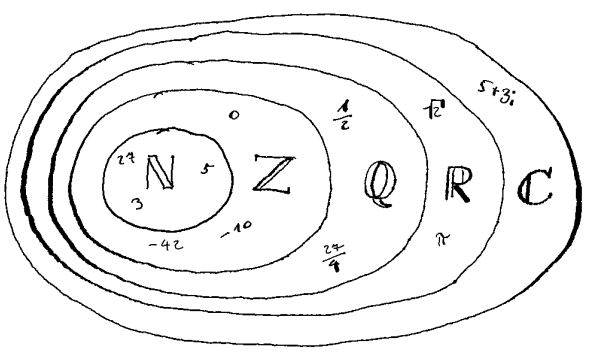
\includegraphics[width=0.6\textwidth]{img/zahlen.png}
    \caption{Zahlen als Euler Diagramm. }
    \label{fig:zahlen}
\end{figure}



Die Arten Mengen in Beziehung zu setzen kann verwendet werden um die unterschiedlichen Zahlen Korpora in Beziehung zu setzen:

$$
\mathbb{N} \subset \mathbb{Z} \subset \mathbb{Q} \subset \mathbb{R} \subset \mathbb{C}
 $$

Siehe auch Abbildung \ref{fig:zahlen}. Im Folgenden ein paar Worte zu den unterschiedlichen Mengen.



\subsection{Natürliche Zahlen $\mathbb{N}$}
Ganzzahlen beginnend bei $1$. Also $\{1,2,3,4,...\}$. Manchmal wir hier die Zahl $0$ inkludiert wenn es in dem Zusammenhang praktisch ist. Dies wird typischerweise so markiert: $\mathbb{N}_0$.  
\subsection{Ganze Zahlen $\mathbb{Z}$}
Alle Ganzzahlen inkl. $0$ und negativen Zahlen.
\subsection{Rationale Zahlen $\mathbb{Q}$}
Zahlen die als Brüche von Ganzzahlen ausgedrückt werden können. zB. $5$ $\frac{1}{2}$ oder $\frac{1}{3}$.

\subsection{Reelle Zahlen $\mathbb{R}$}
\index{Reelle Zahlen}
Reelle Zahlen füllen die 'Lücken' zwischen den Rationalen Zahlen. Enthalten sind auch irrationale Zahlen wie $\pi$ oder $\sqrt{2}$.



\begin{figure}[h!]
    \centering
    

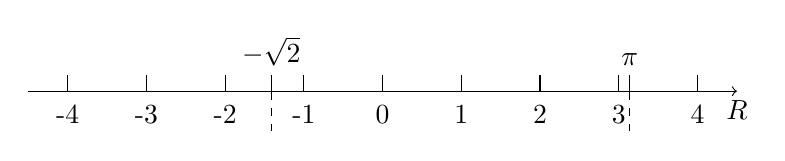
\begin{tikzpicture}
    % Draw the number line from -4 to 4
    \draw[->] (-4.5,0) -- (4.5,0) node[below] {$\mathbb{R}$}; % The real number line
    
    % Draw ticks at whole number intervals
    \foreach \x in {-4,-3,-2,-1,0,1,2,3,4}
      \draw (\x,0) -- (\x,0.2);
      
    % Label the whole numbers below the number line
    \foreach \x in {-4,-3,-2,-1,0,1,2,3,4}
      \node at (\x,-0.3) {\x};

    % Mark and label pi above
    \draw (3.14,0) -- (3.14,0.2) node[above] {$\pi$};
    
    % Mark and label -sqrt(2) above
    \draw (-1.414,0) -- (-1.414,0.2) node[above] {$-\sqrt{2}$};
    
    % Add dashed lines for pi and -sqrt(2)
    \draw[dashed] (3.14,0) -- (3.14,-0.5);
    \draw[dashed] (-1.414,0) -- (-1.414,-0.5);

\end{tikzpicture}
    \caption{Zahlengerade.}
    \label{fig:zahlengerade}
\end{figure}


\subsection{Komplexe Zahlen $\mathbb{C}$}
Besonders wichtig für die Tontechnik, hierzu mehr in Kapitel \ref{chap:complex}. Erweiterung der Zahlengeraden (siehe Abb. \ref{fig:zahlengerade}) auf die 'Komplexe Ebene'. Sie dienen uns zur Darstellung von Schwingungen, kommen vor in der Fouriertransformation (bei jeder Berechnung eines klassischen Audio Spektrums!) etc. \
Es gibt noch weitere Zahlen Mengen, zum Beispiel die \emph{Quaternionen}, eine Erweiterung der Komplexen Zahlen. Diese finden zum Beispiel Anwendung in der Grafik Verarbeitung (in mehr oder weniger jeder 3D Animation zB.). 


\todo[inline]{Intervalle?}

\section{Rechenoperationen}

Einfache Rechenoperationen wie $+, -, \cdot, / $, haben in der Tontechnik/Signalverarbeitung direkt fassbare Bedeutungen.


\begin{figure}[h!]
    \centering
        %% Creator: Matplotlib, PGF backend
%%
%% To include the figure in your LaTeX document, write
%%   \input{<filename>.pgf}
%%
%% Make sure the required packages are loaded in your preamble
%%   \usepackage{pgf}
%%
%% Also ensure that all the required font packages are loaded; for instance,
%% the lmodern package is sometimes necessary when using math font.
%%   \usepackage{lmodern}
%%
%% Figures using additional raster images can only be included by \input if
%% they are in the same directory as the main LaTeX file. For loading figures
%% from other directories you can use the `import` package
%%   \usepackage{import}
%%
%% and then include the figures with
%%   \import{<path to file>}{<filename>.pgf}
%%
%% Matplotlib used the following preamble
%%   \def\mathdefault#1{#1}
%%   \everymath=\expandafter{\the\everymath\displaystyle}
%%   
%%   \usepackage{fontspec}
%%   \setmainfont{VeraSe.ttf}[Path=\detokenize{/usr/share/fonts/TTF/}]
%%   \setsansfont{DejaVuSans.ttf}[Path=\detokenize{/home/pl/miniconda3/lib/python3.12/site-packages/matplotlib/mpl-data/fonts/ttf/}]
%%   \setmonofont{DejaVuSansMono.ttf}[Path=\detokenize{/home/pl/miniconda3/lib/python3.12/site-packages/matplotlib/mpl-data/fonts/ttf/}]
%%   \makeatletter\@ifpackageloaded{underscore}{}{\usepackage[strings]{underscore}}\makeatother
%%
\begingroup%
\makeatletter%
\begin{pgfpicture}%
\pgfpathrectangle{\pgfpointorigin}{\pgfqpoint{6.093662in}{2.027596in}}%
\pgfusepath{use as bounding box, clip}%
\begin{pgfscope}%
\pgfsetbuttcap%
\pgfsetmiterjoin%
\definecolor{currentfill}{rgb}{1.000000,1.000000,1.000000}%
\pgfsetfillcolor{currentfill}%
\pgfsetlinewidth{0.000000pt}%
\definecolor{currentstroke}{rgb}{1.000000,1.000000,1.000000}%
\pgfsetstrokecolor{currentstroke}%
\pgfsetdash{}{0pt}%
\pgfpathmoveto{\pgfqpoint{0.000000in}{0.000000in}}%
\pgfpathlineto{\pgfqpoint{6.093662in}{0.000000in}}%
\pgfpathlineto{\pgfqpoint{6.093662in}{2.027596in}}%
\pgfpathlineto{\pgfqpoint{0.000000in}{2.027596in}}%
\pgfpathlineto{\pgfqpoint{0.000000in}{0.000000in}}%
\pgfpathclose%
\pgfusepath{fill}%
\end{pgfscope}%
\begin{pgfscope}%
\pgfsetbuttcap%
\pgfsetmiterjoin%
\definecolor{currentfill}{rgb}{1.000000,1.000000,1.000000}%
\pgfsetfillcolor{currentfill}%
\pgfsetlinewidth{0.000000pt}%
\definecolor{currentstroke}{rgb}{0.000000,0.000000,0.000000}%
\pgfsetstrokecolor{currentstroke}%
\pgfsetstrokeopacity{0.000000}%
\pgfsetdash{}{0pt}%
\pgfpathmoveto{\pgfqpoint{0.526127in}{0.331635in}}%
\pgfpathlineto{\pgfqpoint{2.992036in}{0.331635in}}%
\pgfpathlineto{\pgfqpoint{2.992036in}{1.717635in}}%
\pgfpathlineto{\pgfqpoint{0.526127in}{1.717635in}}%
\pgfpathlineto{\pgfqpoint{0.526127in}{0.331635in}}%
\pgfpathclose%
\pgfusepath{fill}%
\end{pgfscope}%
\begin{pgfscope}%
\pgfsetbuttcap%
\pgfsetroundjoin%
\definecolor{currentfill}{rgb}{0.000000,0.000000,0.000000}%
\pgfsetfillcolor{currentfill}%
\pgfsetlinewidth{0.803000pt}%
\definecolor{currentstroke}{rgb}{0.000000,0.000000,0.000000}%
\pgfsetstrokecolor{currentstroke}%
\pgfsetdash{}{0pt}%
\pgfsys@defobject{currentmarker}{\pgfqpoint{0.000000in}{-0.048611in}}{\pgfqpoint{0.000000in}{0.000000in}}{%
\pgfpathmoveto{\pgfqpoint{0.000000in}{0.000000in}}%
\pgfpathlineto{\pgfqpoint{0.000000in}{-0.048611in}}%
\pgfusepath{stroke,fill}%
}%
\begin{pgfscope}%
\pgfsys@transformshift{0.638213in}{0.331635in}%
\pgfsys@useobject{currentmarker}{}%
\end{pgfscope}%
\end{pgfscope}%
\begin{pgfscope}%
\definecolor{textcolor}{rgb}{0.000000,0.000000,0.000000}%
\pgfsetstrokecolor{textcolor}%
\pgfsetfillcolor{textcolor}%
\pgftext[x=0.638213in,y=0.234413in,,top]{\color{textcolor}{\rmfamily\fontsize{10.000000}{12.000000}\selectfont\catcode`\^=\active\def^{\ifmmode\sp\else\^{}\fi}\catcode`\%=\active\def%{\%}0.00}}%
\end{pgfscope}%
\begin{pgfscope}%
\pgfsetbuttcap%
\pgfsetroundjoin%
\definecolor{currentfill}{rgb}{0.000000,0.000000,0.000000}%
\pgfsetfillcolor{currentfill}%
\pgfsetlinewidth{0.803000pt}%
\definecolor{currentstroke}{rgb}{0.000000,0.000000,0.000000}%
\pgfsetstrokecolor{currentstroke}%
\pgfsetdash{}{0pt}%
\pgfsys@defobject{currentmarker}{\pgfqpoint{0.000000in}{-0.048611in}}{\pgfqpoint{0.000000in}{0.000000in}}{%
\pgfpathmoveto{\pgfqpoint{0.000000in}{0.000000in}}%
\pgfpathlineto{\pgfqpoint{0.000000in}{-0.048611in}}%
\pgfusepath{stroke,fill}%
}%
\begin{pgfscope}%
\pgfsys@transformshift{1.198647in}{0.331635in}%
\pgfsys@useobject{currentmarker}{}%
\end{pgfscope}%
\end{pgfscope}%
\begin{pgfscope}%
\definecolor{textcolor}{rgb}{0.000000,0.000000,0.000000}%
\pgfsetstrokecolor{textcolor}%
\pgfsetfillcolor{textcolor}%
\pgftext[x=1.198647in,y=0.234413in,,top]{\color{textcolor}{\rmfamily\fontsize{10.000000}{12.000000}\selectfont\catcode`\^=\active\def^{\ifmmode\sp\else\^{}\fi}\catcode`\%=\active\def%{\%}0.25}}%
\end{pgfscope}%
\begin{pgfscope}%
\pgfsetbuttcap%
\pgfsetroundjoin%
\definecolor{currentfill}{rgb}{0.000000,0.000000,0.000000}%
\pgfsetfillcolor{currentfill}%
\pgfsetlinewidth{0.803000pt}%
\definecolor{currentstroke}{rgb}{0.000000,0.000000,0.000000}%
\pgfsetstrokecolor{currentstroke}%
\pgfsetdash{}{0pt}%
\pgfsys@defobject{currentmarker}{\pgfqpoint{0.000000in}{-0.048611in}}{\pgfqpoint{0.000000in}{0.000000in}}{%
\pgfpathmoveto{\pgfqpoint{0.000000in}{0.000000in}}%
\pgfpathlineto{\pgfqpoint{0.000000in}{-0.048611in}}%
\pgfusepath{stroke,fill}%
}%
\begin{pgfscope}%
\pgfsys@transformshift{1.759081in}{0.331635in}%
\pgfsys@useobject{currentmarker}{}%
\end{pgfscope}%
\end{pgfscope}%
\begin{pgfscope}%
\definecolor{textcolor}{rgb}{0.000000,0.000000,0.000000}%
\pgfsetstrokecolor{textcolor}%
\pgfsetfillcolor{textcolor}%
\pgftext[x=1.759081in,y=0.234413in,,top]{\color{textcolor}{\rmfamily\fontsize{10.000000}{12.000000}\selectfont\catcode`\^=\active\def^{\ifmmode\sp\else\^{}\fi}\catcode`\%=\active\def%{\%}0.50}}%
\end{pgfscope}%
\begin{pgfscope}%
\pgfsetbuttcap%
\pgfsetroundjoin%
\definecolor{currentfill}{rgb}{0.000000,0.000000,0.000000}%
\pgfsetfillcolor{currentfill}%
\pgfsetlinewidth{0.803000pt}%
\definecolor{currentstroke}{rgb}{0.000000,0.000000,0.000000}%
\pgfsetstrokecolor{currentstroke}%
\pgfsetdash{}{0pt}%
\pgfsys@defobject{currentmarker}{\pgfqpoint{0.000000in}{-0.048611in}}{\pgfqpoint{0.000000in}{0.000000in}}{%
\pgfpathmoveto{\pgfqpoint{0.000000in}{0.000000in}}%
\pgfpathlineto{\pgfqpoint{0.000000in}{-0.048611in}}%
\pgfusepath{stroke,fill}%
}%
\begin{pgfscope}%
\pgfsys@transformshift{2.319515in}{0.331635in}%
\pgfsys@useobject{currentmarker}{}%
\end{pgfscope}%
\end{pgfscope}%
\begin{pgfscope}%
\definecolor{textcolor}{rgb}{0.000000,0.000000,0.000000}%
\pgfsetstrokecolor{textcolor}%
\pgfsetfillcolor{textcolor}%
\pgftext[x=2.319515in,y=0.234413in,,top]{\color{textcolor}{\rmfamily\fontsize{10.000000}{12.000000}\selectfont\catcode`\^=\active\def^{\ifmmode\sp\else\^{}\fi}\catcode`\%=\active\def%{\%}0.75}}%
\end{pgfscope}%
\begin{pgfscope}%
\pgfsetbuttcap%
\pgfsetroundjoin%
\definecolor{currentfill}{rgb}{0.000000,0.000000,0.000000}%
\pgfsetfillcolor{currentfill}%
\pgfsetlinewidth{0.803000pt}%
\definecolor{currentstroke}{rgb}{0.000000,0.000000,0.000000}%
\pgfsetstrokecolor{currentstroke}%
\pgfsetdash{}{0pt}%
\pgfsys@defobject{currentmarker}{\pgfqpoint{0.000000in}{-0.048611in}}{\pgfqpoint{0.000000in}{0.000000in}}{%
\pgfpathmoveto{\pgfqpoint{0.000000in}{0.000000in}}%
\pgfpathlineto{\pgfqpoint{0.000000in}{-0.048611in}}%
\pgfusepath{stroke,fill}%
}%
\begin{pgfscope}%
\pgfsys@transformshift{2.879949in}{0.331635in}%
\pgfsys@useobject{currentmarker}{}%
\end{pgfscope}%
\end{pgfscope}%
\begin{pgfscope}%
\definecolor{textcolor}{rgb}{0.000000,0.000000,0.000000}%
\pgfsetstrokecolor{textcolor}%
\pgfsetfillcolor{textcolor}%
\pgftext[x=2.879949in,y=0.234413in,,top]{\color{textcolor}{\rmfamily\fontsize{10.000000}{12.000000}\selectfont\catcode`\^=\active\def^{\ifmmode\sp\else\^{}\fi}\catcode`\%=\active\def%{\%}1.00}}%
\end{pgfscope}%
\begin{pgfscope}%
\pgfsetbuttcap%
\pgfsetroundjoin%
\definecolor{currentfill}{rgb}{0.000000,0.000000,0.000000}%
\pgfsetfillcolor{currentfill}%
\pgfsetlinewidth{0.803000pt}%
\definecolor{currentstroke}{rgb}{0.000000,0.000000,0.000000}%
\pgfsetstrokecolor{currentstroke}%
\pgfsetdash{}{0pt}%
\pgfsys@defobject{currentmarker}{\pgfqpoint{-0.048611in}{0.000000in}}{\pgfqpoint{-0.000000in}{0.000000in}}{%
\pgfpathmoveto{\pgfqpoint{-0.000000in}{0.000000in}}%
\pgfpathlineto{\pgfqpoint{-0.048611in}{0.000000in}}%
\pgfusepath{stroke,fill}%
}%
\begin{pgfscope}%
\pgfsys@transformshift{0.526127in}{0.331635in}%
\pgfsys@useobject{currentmarker}{}%
\end{pgfscope}%
\end{pgfscope}%
\begin{pgfscope}%
\definecolor{textcolor}{rgb}{0.000000,0.000000,0.000000}%
\pgfsetstrokecolor{textcolor}%
\pgfsetfillcolor{textcolor}%
\pgftext[x=0.100000in, y=0.278873in, left, base]{\color{textcolor}{\rmfamily\fontsize{10.000000}{12.000000}\selectfont\catcode`\^=\active\def^{\ifmmode\sp\else\^{}\fi}\catcode`\%=\active\def%{\%}\ensuremath{-}1.0}}%
\end{pgfscope}%
\begin{pgfscope}%
\pgfsetbuttcap%
\pgfsetroundjoin%
\definecolor{currentfill}{rgb}{0.000000,0.000000,0.000000}%
\pgfsetfillcolor{currentfill}%
\pgfsetlinewidth{0.803000pt}%
\definecolor{currentstroke}{rgb}{0.000000,0.000000,0.000000}%
\pgfsetstrokecolor{currentstroke}%
\pgfsetdash{}{0pt}%
\pgfsys@defobject{currentmarker}{\pgfqpoint{-0.048611in}{0.000000in}}{\pgfqpoint{-0.000000in}{0.000000in}}{%
\pgfpathmoveto{\pgfqpoint{-0.000000in}{0.000000in}}%
\pgfpathlineto{\pgfqpoint{-0.048611in}{0.000000in}}%
\pgfusepath{stroke,fill}%
}%
\begin{pgfscope}%
\pgfsys@transformshift{0.526127in}{0.678135in}%
\pgfsys@useobject{currentmarker}{}%
\end{pgfscope}%
\end{pgfscope}%
\begin{pgfscope}%
\definecolor{textcolor}{rgb}{0.000000,0.000000,0.000000}%
\pgfsetstrokecolor{textcolor}%
\pgfsetfillcolor{textcolor}%
\pgftext[x=0.100000in, y=0.625373in, left, base]{\color{textcolor}{\rmfamily\fontsize{10.000000}{12.000000}\selectfont\catcode`\^=\active\def^{\ifmmode\sp\else\^{}\fi}\catcode`\%=\active\def%{\%}\ensuremath{-}0.5}}%
\end{pgfscope}%
\begin{pgfscope}%
\pgfsetbuttcap%
\pgfsetroundjoin%
\definecolor{currentfill}{rgb}{0.000000,0.000000,0.000000}%
\pgfsetfillcolor{currentfill}%
\pgfsetlinewidth{0.803000pt}%
\definecolor{currentstroke}{rgb}{0.000000,0.000000,0.000000}%
\pgfsetstrokecolor{currentstroke}%
\pgfsetdash{}{0pt}%
\pgfsys@defobject{currentmarker}{\pgfqpoint{-0.048611in}{0.000000in}}{\pgfqpoint{-0.000000in}{0.000000in}}{%
\pgfpathmoveto{\pgfqpoint{-0.000000in}{0.000000in}}%
\pgfpathlineto{\pgfqpoint{-0.048611in}{0.000000in}}%
\pgfusepath{stroke,fill}%
}%
\begin{pgfscope}%
\pgfsys@transformshift{0.526127in}{1.024635in}%
\pgfsys@useobject{currentmarker}{}%
\end{pgfscope}%
\end{pgfscope}%
\begin{pgfscope}%
\definecolor{textcolor}{rgb}{0.000000,0.000000,0.000000}%
\pgfsetstrokecolor{textcolor}%
\pgfsetfillcolor{textcolor}%
\pgftext[x=0.208025in, y=0.971873in, left, base]{\color{textcolor}{\rmfamily\fontsize{10.000000}{12.000000}\selectfont\catcode`\^=\active\def^{\ifmmode\sp\else\^{}\fi}\catcode`\%=\active\def%{\%}0.0}}%
\end{pgfscope}%
\begin{pgfscope}%
\pgfsetbuttcap%
\pgfsetroundjoin%
\definecolor{currentfill}{rgb}{0.000000,0.000000,0.000000}%
\pgfsetfillcolor{currentfill}%
\pgfsetlinewidth{0.803000pt}%
\definecolor{currentstroke}{rgb}{0.000000,0.000000,0.000000}%
\pgfsetstrokecolor{currentstroke}%
\pgfsetdash{}{0pt}%
\pgfsys@defobject{currentmarker}{\pgfqpoint{-0.048611in}{0.000000in}}{\pgfqpoint{-0.000000in}{0.000000in}}{%
\pgfpathmoveto{\pgfqpoint{-0.000000in}{0.000000in}}%
\pgfpathlineto{\pgfqpoint{-0.048611in}{0.000000in}}%
\pgfusepath{stroke,fill}%
}%
\begin{pgfscope}%
\pgfsys@transformshift{0.526127in}{1.371135in}%
\pgfsys@useobject{currentmarker}{}%
\end{pgfscope}%
\end{pgfscope}%
\begin{pgfscope}%
\definecolor{textcolor}{rgb}{0.000000,0.000000,0.000000}%
\pgfsetstrokecolor{textcolor}%
\pgfsetfillcolor{textcolor}%
\pgftext[x=0.208025in, y=1.318373in, left, base]{\color{textcolor}{\rmfamily\fontsize{10.000000}{12.000000}\selectfont\catcode`\^=\active\def^{\ifmmode\sp\else\^{}\fi}\catcode`\%=\active\def%{\%}0.5}}%
\end{pgfscope}%
\begin{pgfscope}%
\pgfsetbuttcap%
\pgfsetroundjoin%
\definecolor{currentfill}{rgb}{0.000000,0.000000,0.000000}%
\pgfsetfillcolor{currentfill}%
\pgfsetlinewidth{0.803000pt}%
\definecolor{currentstroke}{rgb}{0.000000,0.000000,0.000000}%
\pgfsetstrokecolor{currentstroke}%
\pgfsetdash{}{0pt}%
\pgfsys@defobject{currentmarker}{\pgfqpoint{-0.048611in}{0.000000in}}{\pgfqpoint{-0.000000in}{0.000000in}}{%
\pgfpathmoveto{\pgfqpoint{-0.000000in}{0.000000in}}%
\pgfpathlineto{\pgfqpoint{-0.048611in}{0.000000in}}%
\pgfusepath{stroke,fill}%
}%
\begin{pgfscope}%
\pgfsys@transformshift{0.526127in}{1.717635in}%
\pgfsys@useobject{currentmarker}{}%
\end{pgfscope}%
\end{pgfscope}%
\begin{pgfscope}%
\definecolor{textcolor}{rgb}{0.000000,0.000000,0.000000}%
\pgfsetstrokecolor{textcolor}%
\pgfsetfillcolor{textcolor}%
\pgftext[x=0.208025in, y=1.664873in, left, base]{\color{textcolor}{\rmfamily\fontsize{10.000000}{12.000000}\selectfont\catcode`\^=\active\def^{\ifmmode\sp\else\^{}\fi}\catcode`\%=\active\def%{\%}1.0}}%
\end{pgfscope}%
\begin{pgfscope}%
\pgfpathrectangle{\pgfqpoint{0.526127in}{0.331635in}}{\pgfqpoint{2.465909in}{1.386000in}}%
\pgfusepath{clip}%
\pgfsetrectcap%
\pgfsetroundjoin%
\pgfsetlinewidth{1.505625pt}%
\definecolor{currentstroke}{rgb}{0.000000,0.000000,0.000000}%
\pgfsetstrokecolor{currentstroke}%
\pgfsetdash{}{0pt}%
\pgfpathmoveto{\pgfqpoint{0.638213in}{1.371135in}}%
\pgfpathlineto{\pgfqpoint{0.658551in}{1.445932in}}%
\pgfpathlineto{\pgfqpoint{0.669229in}{1.477008in}}%
\pgfpathlineto{\pgfqpoint{0.677364in}{1.494487in}}%
\pgfpathlineto{\pgfqpoint{0.683974in}{1.504018in}}%
\pgfpathlineto{\pgfqpoint{0.689566in}{1.508539in}}%
\pgfpathlineto{\pgfqpoint{0.694142in}{1.509734in}}%
\pgfpathlineto{\pgfqpoint{0.698718in}{1.508653in}}%
\pgfpathlineto{\pgfqpoint{0.703803in}{1.504803in}}%
\pgfpathlineto{\pgfqpoint{0.709396in}{1.497444in}}%
\pgfpathlineto{\pgfqpoint{0.716006in}{1.484772in}}%
\pgfpathlineto{\pgfqpoint{0.724141in}{1.463894in}}%
\pgfpathlineto{\pgfqpoint{0.734310in}{1.431195in}}%
\pgfpathlineto{\pgfqpoint{0.750580in}{1.370049in}}%
\pgfpathlineto{\pgfqpoint{0.770918in}{1.295426in}}%
\pgfpathlineto{\pgfqpoint{0.781595in}{1.264564in}}%
\pgfpathlineto{\pgfqpoint{0.789730in}{1.247291in}}%
\pgfpathlineto{\pgfqpoint{0.796340in}{1.237947in}}%
\pgfpathlineto{\pgfqpoint{0.801933in}{1.233593in}}%
\pgfpathlineto{\pgfqpoint{0.806509in}{1.232536in}}%
\pgfpathlineto{\pgfqpoint{0.811085in}{1.233757in}}%
\pgfpathlineto{\pgfqpoint{0.816169in}{1.237758in}}%
\pgfpathlineto{\pgfqpoint{0.821762in}{1.245277in}}%
\pgfpathlineto{\pgfqpoint{0.828372in}{1.258124in}}%
\pgfpathlineto{\pgfqpoint{0.836507in}{1.279186in}}%
\pgfpathlineto{\pgfqpoint{0.847184in}{1.313849in}}%
\pgfpathlineto{\pgfqpoint{0.864472in}{1.379229in}}%
\pgfpathlineto{\pgfqpoint{0.883284in}{1.447752in}}%
\pgfpathlineto{\pgfqpoint{0.893453in}{1.477136in}}%
\pgfpathlineto{\pgfqpoint{0.901588in}{1.494577in}}%
\pgfpathlineto{\pgfqpoint{0.908198in}{1.504074in}}%
\pgfpathlineto{\pgfqpoint{0.913791in}{1.508565in}}%
\pgfpathlineto{\pgfqpoint{0.918367in}{1.509735in}}%
\pgfpathlineto{\pgfqpoint{0.922943in}{1.508628in}}%
\pgfpathlineto{\pgfqpoint{0.928027in}{1.504751in}}%
\pgfpathlineto{\pgfqpoint{0.933620in}{1.497362in}}%
\pgfpathlineto{\pgfqpoint{0.940230in}{1.484658in}}%
\pgfpathlineto{\pgfqpoint{0.948365in}{1.463747in}}%
\pgfpathlineto{\pgfqpoint{0.958534in}{1.431017in}}%
\pgfpathlineto{\pgfqpoint{0.974804in}{1.369851in}}%
\pgfpathlineto{\pgfqpoint{0.995142in}{1.295261in}}%
\pgfpathlineto{\pgfqpoint{1.005819in}{1.264438in}}%
\pgfpathlineto{\pgfqpoint{1.013955in}{1.247203in}}%
\pgfpathlineto{\pgfqpoint{1.020564in}{1.237893in}}%
\pgfpathlineto{\pgfqpoint{1.026157in}{1.233569in}}%
\pgfpathlineto{\pgfqpoint{1.030733in}{1.232538in}}%
\pgfpathlineto{\pgfqpoint{1.035309in}{1.233783in}}%
\pgfpathlineto{\pgfqpoint{1.040394in}{1.237812in}}%
\pgfpathlineto{\pgfqpoint{1.045987in}{1.245360in}}%
\pgfpathlineto{\pgfqpoint{1.052596in}{1.258238in}}%
\pgfpathlineto{\pgfqpoint{1.060732in}{1.279334in}}%
\pgfpathlineto{\pgfqpoint{1.071409in}{1.314028in}}%
\pgfpathlineto{\pgfqpoint{1.088696in}{1.379426in}}%
\pgfpathlineto{\pgfqpoint{1.107508in}{1.447916in}}%
\pgfpathlineto{\pgfqpoint{1.117677in}{1.477263in}}%
\pgfpathlineto{\pgfqpoint{1.125813in}{1.494667in}}%
\pgfpathlineto{\pgfqpoint{1.132422in}{1.504130in}}%
\pgfpathlineto{\pgfqpoint{1.138015in}{1.508590in}}%
\pgfpathlineto{\pgfqpoint{1.142591in}{1.509735in}}%
\pgfpathlineto{\pgfqpoint{1.147167in}{1.508603in}}%
\pgfpathlineto{\pgfqpoint{1.152252in}{1.504699in}}%
\pgfpathlineto{\pgfqpoint{1.157845in}{1.497281in}}%
\pgfpathlineto{\pgfqpoint{1.164454in}{1.484545in}}%
\pgfpathlineto{\pgfqpoint{1.172590in}{1.463600in}}%
\pgfpathlineto{\pgfqpoint{1.182758in}{1.430839in}}%
\pgfpathlineto{\pgfqpoint{1.199029in}{1.369654in}}%
\pgfpathlineto{\pgfqpoint{1.219366in}{1.295095in}}%
\pgfpathlineto{\pgfqpoint{1.230044in}{1.264312in}}%
\pgfpathlineto{\pgfqpoint{1.238179in}{1.247115in}}%
\pgfpathlineto{\pgfqpoint{1.244789in}{1.237839in}}%
\pgfpathlineto{\pgfqpoint{1.250382in}{1.233545in}}%
\pgfpathlineto{\pgfqpoint{1.254958in}{1.232539in}}%
\pgfpathlineto{\pgfqpoint{1.259534in}{1.233810in}}%
\pgfpathlineto{\pgfqpoint{1.264618in}{1.237866in}}%
\pgfpathlineto{\pgfqpoint{1.270211in}{1.245443in}}%
\pgfpathlineto{\pgfqpoint{1.276821in}{1.258353in}}%
\pgfpathlineto{\pgfqpoint{1.284956in}{1.279482in}}%
\pgfpathlineto{\pgfqpoint{1.295633in}{1.314208in}}%
\pgfpathlineto{\pgfqpoint{1.312920in}{1.379623in}}%
\pgfpathlineto{\pgfqpoint{1.331224in}{1.446430in}}%
\pgfpathlineto{\pgfqpoint{1.341902in}{1.477390in}}%
\pgfpathlineto{\pgfqpoint{1.350037in}{1.494756in}}%
\pgfpathlineto{\pgfqpoint{1.356647in}{1.504185in}}%
\pgfpathlineto{\pgfqpoint{1.362240in}{1.508615in}}%
\pgfpathlineto{\pgfqpoint{1.366816in}{1.509735in}}%
\pgfpathlineto{\pgfqpoint{1.371392in}{1.508578in}}%
\pgfpathlineto{\pgfqpoint{1.376476in}{1.504646in}}%
\pgfpathlineto{\pgfqpoint{1.382069in}{1.497199in}}%
\pgfpathlineto{\pgfqpoint{1.388679in}{1.484431in}}%
\pgfpathlineto{\pgfqpoint{1.396814in}{1.463452in}}%
\pgfpathlineto{\pgfqpoint{1.406983in}{1.430660in}}%
\pgfpathlineto{\pgfqpoint{1.423253in}{1.369456in}}%
\pgfpathlineto{\pgfqpoint{1.443082in}{1.296588in}}%
\pgfpathlineto{\pgfqpoint{1.453760in}{1.265453in}}%
\pgfpathlineto{\pgfqpoint{1.461895in}{1.247918in}}%
\pgfpathlineto{\pgfqpoint{1.468505in}{1.238337in}}%
\pgfpathlineto{\pgfqpoint{1.474098in}{1.233770in}}%
\pgfpathlineto{\pgfqpoint{1.478674in}{1.232537in}}%
\pgfpathlineto{\pgfqpoint{1.483250in}{1.233581in}}%
\pgfpathlineto{\pgfqpoint{1.487826in}{1.236884in}}%
\pgfpathlineto{\pgfqpoint{1.493419in}{1.243908in}}%
\pgfpathlineto{\pgfqpoint{1.500028in}{1.256213in}}%
\pgfpathlineto{\pgfqpoint{1.508163in}{1.276701in}}%
\pgfpathlineto{\pgfqpoint{1.518332in}{1.309036in}}%
\pgfpathlineto{\pgfqpoint{1.534094in}{1.367975in}}%
\pgfpathlineto{\pgfqpoint{1.555449in}{1.446596in}}%
\pgfpathlineto{\pgfqpoint{1.566126in}{1.477517in}}%
\pgfpathlineto{\pgfqpoint{1.574261in}{1.494845in}}%
\pgfpathlineto{\pgfqpoint{1.580871in}{1.504240in}}%
\pgfpathlineto{\pgfqpoint{1.586464in}{1.508640in}}%
\pgfpathlineto{\pgfqpoint{1.591040in}{1.509735in}}%
\pgfpathlineto{\pgfqpoint{1.595616in}{1.508552in}}%
\pgfpathlineto{\pgfqpoint{1.600700in}{1.504592in}}%
\pgfpathlineto{\pgfqpoint{1.606293in}{1.497117in}}%
\pgfpathlineto{\pgfqpoint{1.612903in}{1.484317in}}%
\pgfpathlineto{\pgfqpoint{1.621038in}{1.463305in}}%
\pgfpathlineto{\pgfqpoint{1.631207in}{1.430482in}}%
\pgfpathlineto{\pgfqpoint{1.647477in}{1.369259in}}%
\pgfpathlineto{\pgfqpoint{1.667307in}{1.296421in}}%
\pgfpathlineto{\pgfqpoint{1.677984in}{1.265325in}}%
\pgfpathlineto{\pgfqpoint{1.686119in}{1.247828in}}%
\pgfpathlineto{\pgfqpoint{1.692729in}{1.238280in}}%
\pgfpathlineto{\pgfqpoint{1.698322in}{1.233744in}}%
\pgfpathlineto{\pgfqpoint{1.702898in}{1.232536in}}%
\pgfpathlineto{\pgfqpoint{1.707474in}{1.233605in}}%
\pgfpathlineto{\pgfqpoint{1.712558in}{1.237440in}}%
\pgfpathlineto{\pgfqpoint{1.718151in}{1.244785in}}%
\pgfpathlineto{\pgfqpoint{1.724761in}{1.257442in}}%
\pgfpathlineto{\pgfqpoint{1.732896in}{1.278303in}}%
\pgfpathlineto{\pgfqpoint{1.743065in}{1.310986in}}%
\pgfpathlineto{\pgfqpoint{1.759335in}{1.372123in}}%
\pgfpathlineto{\pgfqpoint{1.779673in}{1.446761in}}%
\pgfpathlineto{\pgfqpoint{1.790351in}{1.477643in}}%
\pgfpathlineto{\pgfqpoint{1.798486in}{1.494934in}}%
\pgfpathlineto{\pgfqpoint{1.805096in}{1.504295in}}%
\pgfpathlineto{\pgfqpoint{1.810688in}{1.508665in}}%
\pgfpathlineto{\pgfqpoint{1.815264in}{1.509734in}}%
\pgfpathlineto{\pgfqpoint{1.819840in}{1.508526in}}%
\pgfpathlineto{\pgfqpoint{1.824925in}{1.504539in}}%
\pgfpathlineto{\pgfqpoint{1.830518in}{1.497034in}}%
\pgfpathlineto{\pgfqpoint{1.837128in}{1.484203in}}%
\pgfpathlineto{\pgfqpoint{1.845263in}{1.463157in}}%
\pgfpathlineto{\pgfqpoint{1.855432in}{1.430303in}}%
\pgfpathlineto{\pgfqpoint{1.871702in}{1.369061in}}%
\pgfpathlineto{\pgfqpoint{1.891531in}{1.296255in}}%
\pgfpathlineto{\pgfqpoint{1.902209in}{1.265198in}}%
\pgfpathlineto{\pgfqpoint{1.910344in}{1.247738in}}%
\pgfpathlineto{\pgfqpoint{1.916953in}{1.238224in}}%
\pgfpathlineto{\pgfqpoint{1.922546in}{1.233718in}}%
\pgfpathlineto{\pgfqpoint{1.927122in}{1.232535in}}%
\pgfpathlineto{\pgfqpoint{1.931698in}{1.233630in}}%
\pgfpathlineto{\pgfqpoint{1.936783in}{1.237493in}}%
\pgfpathlineto{\pgfqpoint{1.942376in}{1.244867in}}%
\pgfpathlineto{\pgfqpoint{1.948986in}{1.257555in}}%
\pgfpathlineto{\pgfqpoint{1.957121in}{1.278450in}}%
\pgfpathlineto{\pgfqpoint{1.967290in}{1.311164in}}%
\pgfpathlineto{\pgfqpoint{1.983560in}{1.372320in}}%
\pgfpathlineto{\pgfqpoint{2.003898in}{1.446927in}}%
\pgfpathlineto{\pgfqpoint{2.014575in}{1.477769in}}%
\pgfpathlineto{\pgfqpoint{2.022710in}{1.495023in}}%
\pgfpathlineto{\pgfqpoint{2.029320in}{1.504350in}}%
\pgfpathlineto{\pgfqpoint{2.034913in}{1.508689in}}%
\pgfpathlineto{\pgfqpoint{2.039489in}{1.509733in}}%
\pgfpathlineto{\pgfqpoint{2.044065in}{1.508500in}}%
\pgfpathlineto{\pgfqpoint{2.049149in}{1.504485in}}%
\pgfpathlineto{\pgfqpoint{2.054742in}{1.496951in}}%
\pgfpathlineto{\pgfqpoint{2.061352in}{1.484089in}}%
\pgfpathlineto{\pgfqpoint{2.069487in}{1.463010in}}%
\pgfpathlineto{\pgfqpoint{2.080164in}{1.428332in}}%
\pgfpathlineto{\pgfqpoint{2.097452in}{1.362943in}}%
\pgfpathlineto{\pgfqpoint{2.116264in}{1.294436in}}%
\pgfpathlineto{\pgfqpoint{2.126433in}{1.265071in}}%
\pgfpathlineto{\pgfqpoint{2.134568in}{1.247648in}}%
\pgfpathlineto{\pgfqpoint{2.141178in}{1.238168in}}%
\pgfpathlineto{\pgfqpoint{2.146771in}{1.233692in}}%
\pgfpathlineto{\pgfqpoint{2.151347in}{1.232535in}}%
\pgfpathlineto{\pgfqpoint{2.155923in}{1.233655in}}%
\pgfpathlineto{\pgfqpoint{2.161007in}{1.237545in}}%
\pgfpathlineto{\pgfqpoint{2.166600in}{1.244948in}}%
\pgfpathlineto{\pgfqpoint{2.173210in}{1.257668in}}%
\pgfpathlineto{\pgfqpoint{2.181345in}{1.278597in}}%
\pgfpathlineto{\pgfqpoint{2.191514in}{1.311342in}}%
\pgfpathlineto{\pgfqpoint{2.207784in}{1.372518in}}%
\pgfpathlineto{\pgfqpoint{2.228122in}{1.447092in}}%
\pgfpathlineto{\pgfqpoint{2.238799in}{1.477895in}}%
\pgfpathlineto{\pgfqpoint{2.246935in}{1.495111in}}%
\pgfpathlineto{\pgfqpoint{2.253544in}{1.504404in}}%
\pgfpathlineto{\pgfqpoint{2.259137in}{1.508713in}}%
\pgfpathlineto{\pgfqpoint{2.263713in}{1.509732in}}%
\pgfpathlineto{\pgfqpoint{2.268289in}{1.508473in}}%
\pgfpathlineto{\pgfqpoint{2.273374in}{1.504431in}}%
\pgfpathlineto{\pgfqpoint{2.278967in}{1.496868in}}%
\pgfpathlineto{\pgfqpoint{2.285576in}{1.483974in}}%
\pgfpathlineto{\pgfqpoint{2.293711in}{1.462862in}}%
\pgfpathlineto{\pgfqpoint{2.304389in}{1.428152in}}%
\pgfpathlineto{\pgfqpoint{2.321676in}{1.362746in}}%
\pgfpathlineto{\pgfqpoint{2.340488in}{1.294272in}}%
\pgfpathlineto{\pgfqpoint{2.350657in}{1.264944in}}%
\pgfpathlineto{\pgfqpoint{2.358792in}{1.247559in}}%
\pgfpathlineto{\pgfqpoint{2.365402in}{1.238113in}}%
\pgfpathlineto{\pgfqpoint{2.370995in}{1.233667in}}%
\pgfpathlineto{\pgfqpoint{2.375571in}{1.232535in}}%
\pgfpathlineto{\pgfqpoint{2.380147in}{1.233680in}}%
\pgfpathlineto{\pgfqpoint{2.385232in}{1.237598in}}%
\pgfpathlineto{\pgfqpoint{2.390825in}{1.245030in}}%
\pgfpathlineto{\pgfqpoint{2.397434in}{1.257782in}}%
\pgfpathlineto{\pgfqpoint{2.405569in}{1.278744in}}%
\pgfpathlineto{\pgfqpoint{2.415738in}{1.311520in}}%
\pgfpathlineto{\pgfqpoint{2.432009in}{1.372715in}}%
\pgfpathlineto{\pgfqpoint{2.452346in}{1.447257in}}%
\pgfpathlineto{\pgfqpoint{2.463024in}{1.478021in}}%
\pgfpathlineto{\pgfqpoint{2.471159in}{1.495199in}}%
\pgfpathlineto{\pgfqpoint{2.477769in}{1.504458in}}%
\pgfpathlineto{\pgfqpoint{2.483362in}{1.508737in}}%
\pgfpathlineto{\pgfqpoint{2.487938in}{1.509730in}}%
\pgfpathlineto{\pgfqpoint{2.492514in}{1.508447in}}%
\pgfpathlineto{\pgfqpoint{2.497598in}{1.504377in}}%
\pgfpathlineto{\pgfqpoint{2.503191in}{1.496785in}}%
\pgfpathlineto{\pgfqpoint{2.509801in}{1.483860in}}%
\pgfpathlineto{\pgfqpoint{2.517936in}{1.462714in}}%
\pgfpathlineto{\pgfqpoint{2.528613in}{1.427971in}}%
\pgfpathlineto{\pgfqpoint{2.545900in}{1.362549in}}%
\pgfpathlineto{\pgfqpoint{2.564204in}{1.295757in}}%
\pgfpathlineto{\pgfqpoint{2.574882in}{1.264817in}}%
\pgfpathlineto{\pgfqpoint{2.583017in}{1.247469in}}%
\pgfpathlineto{\pgfqpoint{2.589627in}{1.238057in}}%
\pgfpathlineto{\pgfqpoint{2.595220in}{1.233642in}}%
\pgfpathlineto{\pgfqpoint{2.599796in}{1.232535in}}%
\pgfpathlineto{\pgfqpoint{2.604372in}{1.233705in}}%
\pgfpathlineto{\pgfqpoint{2.609456in}{1.237651in}}%
\pgfpathlineto{\pgfqpoint{2.615049in}{1.245112in}}%
\pgfpathlineto{\pgfqpoint{2.621659in}{1.257896in}}%
\pgfpathlineto{\pgfqpoint{2.629794in}{1.278891in}}%
\pgfpathlineto{\pgfqpoint{2.639963in}{1.311699in}}%
\pgfpathlineto{\pgfqpoint{2.656233in}{1.372913in}}%
\pgfpathlineto{\pgfqpoint{2.676062in}{1.445765in}}%
\pgfpathlineto{\pgfqpoint{2.686740in}{1.476881in}}%
\pgfpathlineto{\pgfqpoint{2.694875in}{1.494397in}}%
\pgfpathlineto{\pgfqpoint{2.701485in}{1.503962in}}%
\pgfpathlineto{\pgfqpoint{2.707078in}{1.508513in}}%
\pgfpathlineto{\pgfqpoint{2.711654in}{1.509734in}}%
\pgfpathlineto{\pgfqpoint{2.716230in}{1.508677in}}%
\pgfpathlineto{\pgfqpoint{2.720806in}{1.505361in}}%
\pgfpathlineto{\pgfqpoint{2.726398in}{1.498323in}}%
\pgfpathlineto{\pgfqpoint{2.733008in}{1.486002in}}%
\pgfpathlineto{\pgfqpoint{2.741143in}{1.465497in}}%
\pgfpathlineto{\pgfqpoint{2.751312in}{1.433146in}}%
\pgfpathlineto{\pgfqpoint{2.767074in}{1.374196in}}%
\pgfpathlineto{\pgfqpoint{2.788429in}{1.295591in}}%
\pgfpathlineto{\pgfqpoint{2.799106in}{1.264690in}}%
\pgfpathlineto{\pgfqpoint{2.807241in}{1.247380in}}%
\pgfpathlineto{\pgfqpoint{2.813851in}{1.238002in}}%
\pgfpathlineto{\pgfqpoint{2.819444in}{1.233617in}}%
\pgfpathlineto{\pgfqpoint{2.824020in}{1.232536in}}%
\pgfpathlineto{\pgfqpoint{2.828596in}{1.233731in}}%
\pgfpathlineto{\pgfqpoint{2.833680in}{1.237704in}}%
\pgfpathlineto{\pgfqpoint{2.839273in}{1.245195in}}%
\pgfpathlineto{\pgfqpoint{2.845883in}{1.258010in}}%
\pgfpathlineto{\pgfqpoint{2.854018in}{1.279039in}}%
\pgfpathlineto{\pgfqpoint{2.864187in}{1.311877in}}%
\pgfpathlineto{\pgfqpoint{2.879949in}{1.371135in}}%
\pgfpathlineto{\pgfqpoint{2.879949in}{1.371135in}}%
\pgfusepath{stroke}%
\end{pgfscope}%
\begin{pgfscope}%
\pgfpathrectangle{\pgfqpoint{0.526127in}{0.331635in}}{\pgfqpoint{2.465909in}{1.386000in}}%
\pgfusepath{clip}%
\pgfsetrectcap%
\pgfsetroundjoin%
\pgfsetlinewidth{0.501875pt}%
\definecolor{currentstroke}{rgb}{0.000000,0.000000,0.000000}%
\pgfsetstrokecolor{currentstroke}%
\pgfsetdash{}{0pt}%
\pgfpathmoveto{\pgfqpoint{0.526127in}{1.024635in}}%
\pgfpathlineto{\pgfqpoint{2.992036in}{1.024635in}}%
\pgfusepath{stroke}%
\end{pgfscope}%
\begin{pgfscope}%
\definecolor{textcolor}{rgb}{0.000000,0.000000,0.000000}%
\pgfsetstrokecolor{textcolor}%
\pgfsetfillcolor{textcolor}%
\pgftext[x=1.759081in,y=1.800968in,,base]{\color{textcolor}{\rmfamily\fontsize{12.000000}{14.400000}\selectfont\catcode`\^=\active\def^{\ifmmode\sp\else\^{}\fi}\catcode`\%=\active\def%{\%}Signal A}}%
\end{pgfscope}%
\begin{pgfscope}%
\pgfsetbuttcap%
\pgfsetmiterjoin%
\definecolor{currentfill}{rgb}{1.000000,1.000000,1.000000}%
\pgfsetfillcolor{currentfill}%
\pgfsetlinewidth{0.000000pt}%
\definecolor{currentstroke}{rgb}{0.000000,0.000000,0.000000}%
\pgfsetstrokecolor{currentstroke}%
\pgfsetstrokeopacity{0.000000}%
\pgfsetdash{}{0pt}%
\pgfpathmoveto{\pgfqpoint{3.485218in}{0.331635in}}%
\pgfpathlineto{\pgfqpoint{5.951127in}{0.331635in}}%
\pgfpathlineto{\pgfqpoint{5.951127in}{1.717635in}}%
\pgfpathlineto{\pgfqpoint{3.485218in}{1.717635in}}%
\pgfpathlineto{\pgfqpoint{3.485218in}{0.331635in}}%
\pgfpathclose%
\pgfusepath{fill}%
\end{pgfscope}%
\begin{pgfscope}%
\pgfsetbuttcap%
\pgfsetroundjoin%
\definecolor{currentfill}{rgb}{0.000000,0.000000,0.000000}%
\pgfsetfillcolor{currentfill}%
\pgfsetlinewidth{0.803000pt}%
\definecolor{currentstroke}{rgb}{0.000000,0.000000,0.000000}%
\pgfsetstrokecolor{currentstroke}%
\pgfsetdash{}{0pt}%
\pgfsys@defobject{currentmarker}{\pgfqpoint{0.000000in}{-0.048611in}}{\pgfqpoint{0.000000in}{0.000000in}}{%
\pgfpathmoveto{\pgfqpoint{0.000000in}{0.000000in}}%
\pgfpathlineto{\pgfqpoint{0.000000in}{-0.048611in}}%
\pgfusepath{stroke,fill}%
}%
\begin{pgfscope}%
\pgfsys@transformshift{3.597304in}{0.331635in}%
\pgfsys@useobject{currentmarker}{}%
\end{pgfscope}%
\end{pgfscope}%
\begin{pgfscope}%
\definecolor{textcolor}{rgb}{0.000000,0.000000,0.000000}%
\pgfsetstrokecolor{textcolor}%
\pgfsetfillcolor{textcolor}%
\pgftext[x=3.597304in,y=0.234413in,,top]{\color{textcolor}{\rmfamily\fontsize{10.000000}{12.000000}\selectfont\catcode`\^=\active\def^{\ifmmode\sp\else\^{}\fi}\catcode`\%=\active\def%{\%}0.00}}%
\end{pgfscope}%
\begin{pgfscope}%
\pgfsetbuttcap%
\pgfsetroundjoin%
\definecolor{currentfill}{rgb}{0.000000,0.000000,0.000000}%
\pgfsetfillcolor{currentfill}%
\pgfsetlinewidth{0.803000pt}%
\definecolor{currentstroke}{rgb}{0.000000,0.000000,0.000000}%
\pgfsetstrokecolor{currentstroke}%
\pgfsetdash{}{0pt}%
\pgfsys@defobject{currentmarker}{\pgfqpoint{0.000000in}{-0.048611in}}{\pgfqpoint{0.000000in}{0.000000in}}{%
\pgfpathmoveto{\pgfqpoint{0.000000in}{0.000000in}}%
\pgfpathlineto{\pgfqpoint{0.000000in}{-0.048611in}}%
\pgfusepath{stroke,fill}%
}%
\begin{pgfscope}%
\pgfsys@transformshift{4.157738in}{0.331635in}%
\pgfsys@useobject{currentmarker}{}%
\end{pgfscope}%
\end{pgfscope}%
\begin{pgfscope}%
\definecolor{textcolor}{rgb}{0.000000,0.000000,0.000000}%
\pgfsetstrokecolor{textcolor}%
\pgfsetfillcolor{textcolor}%
\pgftext[x=4.157738in,y=0.234413in,,top]{\color{textcolor}{\rmfamily\fontsize{10.000000}{12.000000}\selectfont\catcode`\^=\active\def^{\ifmmode\sp\else\^{}\fi}\catcode`\%=\active\def%{\%}0.25}}%
\end{pgfscope}%
\begin{pgfscope}%
\pgfsetbuttcap%
\pgfsetroundjoin%
\definecolor{currentfill}{rgb}{0.000000,0.000000,0.000000}%
\pgfsetfillcolor{currentfill}%
\pgfsetlinewidth{0.803000pt}%
\definecolor{currentstroke}{rgb}{0.000000,0.000000,0.000000}%
\pgfsetstrokecolor{currentstroke}%
\pgfsetdash{}{0pt}%
\pgfsys@defobject{currentmarker}{\pgfqpoint{0.000000in}{-0.048611in}}{\pgfqpoint{0.000000in}{0.000000in}}{%
\pgfpathmoveto{\pgfqpoint{0.000000in}{0.000000in}}%
\pgfpathlineto{\pgfqpoint{0.000000in}{-0.048611in}}%
\pgfusepath{stroke,fill}%
}%
\begin{pgfscope}%
\pgfsys@transformshift{4.718172in}{0.331635in}%
\pgfsys@useobject{currentmarker}{}%
\end{pgfscope}%
\end{pgfscope}%
\begin{pgfscope}%
\definecolor{textcolor}{rgb}{0.000000,0.000000,0.000000}%
\pgfsetstrokecolor{textcolor}%
\pgfsetfillcolor{textcolor}%
\pgftext[x=4.718172in,y=0.234413in,,top]{\color{textcolor}{\rmfamily\fontsize{10.000000}{12.000000}\selectfont\catcode`\^=\active\def^{\ifmmode\sp\else\^{}\fi}\catcode`\%=\active\def%{\%}0.50}}%
\end{pgfscope}%
\begin{pgfscope}%
\pgfsetbuttcap%
\pgfsetroundjoin%
\definecolor{currentfill}{rgb}{0.000000,0.000000,0.000000}%
\pgfsetfillcolor{currentfill}%
\pgfsetlinewidth{0.803000pt}%
\definecolor{currentstroke}{rgb}{0.000000,0.000000,0.000000}%
\pgfsetstrokecolor{currentstroke}%
\pgfsetdash{}{0pt}%
\pgfsys@defobject{currentmarker}{\pgfqpoint{0.000000in}{-0.048611in}}{\pgfqpoint{0.000000in}{0.000000in}}{%
\pgfpathmoveto{\pgfqpoint{0.000000in}{0.000000in}}%
\pgfpathlineto{\pgfqpoint{0.000000in}{-0.048611in}}%
\pgfusepath{stroke,fill}%
}%
\begin{pgfscope}%
\pgfsys@transformshift{5.278606in}{0.331635in}%
\pgfsys@useobject{currentmarker}{}%
\end{pgfscope}%
\end{pgfscope}%
\begin{pgfscope}%
\definecolor{textcolor}{rgb}{0.000000,0.000000,0.000000}%
\pgfsetstrokecolor{textcolor}%
\pgfsetfillcolor{textcolor}%
\pgftext[x=5.278606in,y=0.234413in,,top]{\color{textcolor}{\rmfamily\fontsize{10.000000}{12.000000}\selectfont\catcode`\^=\active\def^{\ifmmode\sp\else\^{}\fi}\catcode`\%=\active\def%{\%}0.75}}%
\end{pgfscope}%
\begin{pgfscope}%
\pgfsetbuttcap%
\pgfsetroundjoin%
\definecolor{currentfill}{rgb}{0.000000,0.000000,0.000000}%
\pgfsetfillcolor{currentfill}%
\pgfsetlinewidth{0.803000pt}%
\definecolor{currentstroke}{rgb}{0.000000,0.000000,0.000000}%
\pgfsetstrokecolor{currentstroke}%
\pgfsetdash{}{0pt}%
\pgfsys@defobject{currentmarker}{\pgfqpoint{0.000000in}{-0.048611in}}{\pgfqpoint{0.000000in}{0.000000in}}{%
\pgfpathmoveto{\pgfqpoint{0.000000in}{0.000000in}}%
\pgfpathlineto{\pgfqpoint{0.000000in}{-0.048611in}}%
\pgfusepath{stroke,fill}%
}%
\begin{pgfscope}%
\pgfsys@transformshift{5.839040in}{0.331635in}%
\pgfsys@useobject{currentmarker}{}%
\end{pgfscope}%
\end{pgfscope}%
\begin{pgfscope}%
\definecolor{textcolor}{rgb}{0.000000,0.000000,0.000000}%
\pgfsetstrokecolor{textcolor}%
\pgfsetfillcolor{textcolor}%
\pgftext[x=5.839040in,y=0.234413in,,top]{\color{textcolor}{\rmfamily\fontsize{10.000000}{12.000000}\selectfont\catcode`\^=\active\def^{\ifmmode\sp\else\^{}\fi}\catcode`\%=\active\def%{\%}1.00}}%
\end{pgfscope}%
\begin{pgfscope}%
\pgfsetbuttcap%
\pgfsetroundjoin%
\definecolor{currentfill}{rgb}{0.000000,0.000000,0.000000}%
\pgfsetfillcolor{currentfill}%
\pgfsetlinewidth{0.803000pt}%
\definecolor{currentstroke}{rgb}{0.000000,0.000000,0.000000}%
\pgfsetstrokecolor{currentstroke}%
\pgfsetdash{}{0pt}%
\pgfsys@defobject{currentmarker}{\pgfqpoint{-0.048611in}{0.000000in}}{\pgfqpoint{-0.000000in}{0.000000in}}{%
\pgfpathmoveto{\pgfqpoint{-0.000000in}{0.000000in}}%
\pgfpathlineto{\pgfqpoint{-0.048611in}{0.000000in}}%
\pgfusepath{stroke,fill}%
}%
\begin{pgfscope}%
\pgfsys@transformshift{3.485218in}{0.331635in}%
\pgfsys@useobject{currentmarker}{}%
\end{pgfscope}%
\end{pgfscope}%
\begin{pgfscope}%
\definecolor{textcolor}{rgb}{0.000000,0.000000,0.000000}%
\pgfsetstrokecolor{textcolor}%
\pgfsetfillcolor{textcolor}%
\pgftext[x=3.059091in, y=0.278873in, left, base]{\color{textcolor}{\rmfamily\fontsize{10.000000}{12.000000}\selectfont\catcode`\^=\active\def^{\ifmmode\sp\else\^{}\fi}\catcode`\%=\active\def%{\%}\ensuremath{-}1.0}}%
\end{pgfscope}%
\begin{pgfscope}%
\pgfsetbuttcap%
\pgfsetroundjoin%
\definecolor{currentfill}{rgb}{0.000000,0.000000,0.000000}%
\pgfsetfillcolor{currentfill}%
\pgfsetlinewidth{0.803000pt}%
\definecolor{currentstroke}{rgb}{0.000000,0.000000,0.000000}%
\pgfsetstrokecolor{currentstroke}%
\pgfsetdash{}{0pt}%
\pgfsys@defobject{currentmarker}{\pgfqpoint{-0.048611in}{0.000000in}}{\pgfqpoint{-0.000000in}{0.000000in}}{%
\pgfpathmoveto{\pgfqpoint{-0.000000in}{0.000000in}}%
\pgfpathlineto{\pgfqpoint{-0.048611in}{0.000000in}}%
\pgfusepath{stroke,fill}%
}%
\begin{pgfscope}%
\pgfsys@transformshift{3.485218in}{0.678135in}%
\pgfsys@useobject{currentmarker}{}%
\end{pgfscope}%
\end{pgfscope}%
\begin{pgfscope}%
\definecolor{textcolor}{rgb}{0.000000,0.000000,0.000000}%
\pgfsetstrokecolor{textcolor}%
\pgfsetfillcolor{textcolor}%
\pgftext[x=3.059091in, y=0.625373in, left, base]{\color{textcolor}{\rmfamily\fontsize{10.000000}{12.000000}\selectfont\catcode`\^=\active\def^{\ifmmode\sp\else\^{}\fi}\catcode`\%=\active\def%{\%}\ensuremath{-}0.5}}%
\end{pgfscope}%
\begin{pgfscope}%
\pgfsetbuttcap%
\pgfsetroundjoin%
\definecolor{currentfill}{rgb}{0.000000,0.000000,0.000000}%
\pgfsetfillcolor{currentfill}%
\pgfsetlinewidth{0.803000pt}%
\definecolor{currentstroke}{rgb}{0.000000,0.000000,0.000000}%
\pgfsetstrokecolor{currentstroke}%
\pgfsetdash{}{0pt}%
\pgfsys@defobject{currentmarker}{\pgfqpoint{-0.048611in}{0.000000in}}{\pgfqpoint{-0.000000in}{0.000000in}}{%
\pgfpathmoveto{\pgfqpoint{-0.000000in}{0.000000in}}%
\pgfpathlineto{\pgfqpoint{-0.048611in}{0.000000in}}%
\pgfusepath{stroke,fill}%
}%
\begin{pgfscope}%
\pgfsys@transformshift{3.485218in}{1.024635in}%
\pgfsys@useobject{currentmarker}{}%
\end{pgfscope}%
\end{pgfscope}%
\begin{pgfscope}%
\definecolor{textcolor}{rgb}{0.000000,0.000000,0.000000}%
\pgfsetstrokecolor{textcolor}%
\pgfsetfillcolor{textcolor}%
\pgftext[x=3.167116in, y=0.971873in, left, base]{\color{textcolor}{\rmfamily\fontsize{10.000000}{12.000000}\selectfont\catcode`\^=\active\def^{\ifmmode\sp\else\^{}\fi}\catcode`\%=\active\def%{\%}0.0}}%
\end{pgfscope}%
\begin{pgfscope}%
\pgfsetbuttcap%
\pgfsetroundjoin%
\definecolor{currentfill}{rgb}{0.000000,0.000000,0.000000}%
\pgfsetfillcolor{currentfill}%
\pgfsetlinewidth{0.803000pt}%
\definecolor{currentstroke}{rgb}{0.000000,0.000000,0.000000}%
\pgfsetstrokecolor{currentstroke}%
\pgfsetdash{}{0pt}%
\pgfsys@defobject{currentmarker}{\pgfqpoint{-0.048611in}{0.000000in}}{\pgfqpoint{-0.000000in}{0.000000in}}{%
\pgfpathmoveto{\pgfqpoint{-0.000000in}{0.000000in}}%
\pgfpathlineto{\pgfqpoint{-0.048611in}{0.000000in}}%
\pgfusepath{stroke,fill}%
}%
\begin{pgfscope}%
\pgfsys@transformshift{3.485218in}{1.371135in}%
\pgfsys@useobject{currentmarker}{}%
\end{pgfscope}%
\end{pgfscope}%
\begin{pgfscope}%
\definecolor{textcolor}{rgb}{0.000000,0.000000,0.000000}%
\pgfsetstrokecolor{textcolor}%
\pgfsetfillcolor{textcolor}%
\pgftext[x=3.167116in, y=1.318373in, left, base]{\color{textcolor}{\rmfamily\fontsize{10.000000}{12.000000}\selectfont\catcode`\^=\active\def^{\ifmmode\sp\else\^{}\fi}\catcode`\%=\active\def%{\%}0.5}}%
\end{pgfscope}%
\begin{pgfscope}%
\pgfsetbuttcap%
\pgfsetroundjoin%
\definecolor{currentfill}{rgb}{0.000000,0.000000,0.000000}%
\pgfsetfillcolor{currentfill}%
\pgfsetlinewidth{0.803000pt}%
\definecolor{currentstroke}{rgb}{0.000000,0.000000,0.000000}%
\pgfsetstrokecolor{currentstroke}%
\pgfsetdash{}{0pt}%
\pgfsys@defobject{currentmarker}{\pgfqpoint{-0.048611in}{0.000000in}}{\pgfqpoint{-0.000000in}{0.000000in}}{%
\pgfpathmoveto{\pgfqpoint{-0.000000in}{0.000000in}}%
\pgfpathlineto{\pgfqpoint{-0.048611in}{0.000000in}}%
\pgfusepath{stroke,fill}%
}%
\begin{pgfscope}%
\pgfsys@transformshift{3.485218in}{1.717635in}%
\pgfsys@useobject{currentmarker}{}%
\end{pgfscope}%
\end{pgfscope}%
\begin{pgfscope}%
\definecolor{textcolor}{rgb}{0.000000,0.000000,0.000000}%
\pgfsetstrokecolor{textcolor}%
\pgfsetfillcolor{textcolor}%
\pgftext[x=3.167116in, y=1.664873in, left, base]{\color{textcolor}{\rmfamily\fontsize{10.000000}{12.000000}\selectfont\catcode`\^=\active\def^{\ifmmode\sp\else\^{}\fi}\catcode`\%=\active\def%{\%}1.0}}%
\end{pgfscope}%
\begin{pgfscope}%
\pgfpathrectangle{\pgfqpoint{3.485218in}{0.331635in}}{\pgfqpoint{2.465909in}{1.386000in}}%
\pgfusepath{clip}%
\pgfsetrectcap%
\pgfsetroundjoin%
\pgfsetlinewidth{1.505625pt}%
\definecolor{currentstroke}{rgb}{0.000000,0.000000,0.000000}%
\pgfsetstrokecolor{currentstroke}%
\pgfsetdash{}{0pt}%
\pgfpathmoveto{\pgfqpoint{3.597304in}{1.024635in}}%
\pgfpathlineto{\pgfqpoint{3.704078in}{1.126790in}}%
\pgfpathlineto{\pgfqpoint{3.761024in}{1.178114in}}%
\pgfpathlineto{\pgfqpoint{3.808309in}{1.217820in}}%
\pgfpathlineto{\pgfqpoint{3.850510in}{1.250414in}}%
\pgfpathlineto{\pgfqpoint{3.889152in}{1.277503in}}%
\pgfpathlineto{\pgfqpoint{3.925252in}{1.300138in}}%
\pgfpathlineto{\pgfqpoint{3.959317in}{1.318918in}}%
\pgfpathlineto{\pgfqpoint{3.991858in}{1.334355in}}%
\pgfpathlineto{\pgfqpoint{4.023382in}{1.346855in}}%
\pgfpathlineto{\pgfqpoint{4.053888in}{1.356560in}}%
\pgfpathlineto{\pgfqpoint{4.083378in}{1.363637in}}%
\pgfpathlineto{\pgfqpoint{4.112359in}{1.368336in}}%
\pgfpathlineto{\pgfqpoint{4.141341in}{1.370769in}}%
\pgfpathlineto{\pgfqpoint{4.169814in}{1.370937in}}%
\pgfpathlineto{\pgfqpoint{4.198287in}{1.368900in}}%
\pgfpathlineto{\pgfqpoint{4.227268in}{1.364576in}}%
\pgfpathlineto{\pgfqpoint{4.256250in}{1.358011in}}%
\pgfpathlineto{\pgfqpoint{4.286248in}{1.348900in}}%
\pgfpathlineto{\pgfqpoint{4.316755in}{1.337286in}}%
\pgfpathlineto{\pgfqpoint{4.348278in}{1.322886in}}%
\pgfpathlineto{\pgfqpoint{4.381327in}{1.305293in}}%
\pgfpathlineto{\pgfqpoint{4.415901in}{1.284315in}}%
\pgfpathlineto{\pgfqpoint{4.452509in}{1.259452in}}%
\pgfpathlineto{\pgfqpoint{4.491660in}{1.230136in}}%
\pgfpathlineto{\pgfqpoint{4.534878in}{1.194919in}}%
\pgfpathlineto{\pgfqpoint{4.583688in}{1.152172in}}%
\pgfpathlineto{\pgfqpoint{4.642668in}{1.097417in}}%
\pgfpathlineto{\pgfqpoint{4.739781in}{1.003662in}}%
\pgfpathlineto{\pgfqpoint{4.828759in}{0.918947in}}%
\pgfpathlineto{\pgfqpoint{4.884688in}{0.868726in}}%
\pgfpathlineto{\pgfqpoint{4.931465in}{0.829610in}}%
\pgfpathlineto{\pgfqpoint{4.973157in}{0.797548in}}%
\pgfpathlineto{\pgfqpoint{5.011799in}{0.770589in}}%
\pgfpathlineto{\pgfqpoint{5.047899in}{0.748087in}}%
\pgfpathlineto{\pgfqpoint{5.081965in}{0.729444in}}%
\pgfpathlineto{\pgfqpoint{5.114505in}{0.714144in}}%
\pgfpathlineto{\pgfqpoint{5.146029in}{0.701783in}}%
\pgfpathlineto{\pgfqpoint{5.176536in}{0.692218in}}%
\pgfpathlineto{\pgfqpoint{5.206025in}{0.685280in}}%
\pgfpathlineto{\pgfqpoint{5.235007in}{0.680719in}}%
\pgfpathlineto{\pgfqpoint{5.263988in}{0.678426in}}%
\pgfpathlineto{\pgfqpoint{5.292461in}{0.678396in}}%
\pgfpathlineto{\pgfqpoint{5.320934in}{0.680571in}}%
\pgfpathlineto{\pgfqpoint{5.349915in}{0.685033in}}%
\pgfpathlineto{\pgfqpoint{5.378897in}{0.691735in}}%
\pgfpathlineto{\pgfqpoint{5.408895in}{0.700983in}}%
\pgfpathlineto{\pgfqpoint{5.439402in}{0.712733in}}%
\pgfpathlineto{\pgfqpoint{5.470925in}{0.727268in}}%
\pgfpathlineto{\pgfqpoint{5.503974in}{0.744994in}}%
\pgfpathlineto{\pgfqpoint{5.538549in}{0.766103in}}%
\pgfpathlineto{\pgfqpoint{5.575157in}{0.791092in}}%
\pgfpathlineto{\pgfqpoint{5.614815in}{0.820927in}}%
\pgfpathlineto{\pgfqpoint{5.658033in}{0.856290in}}%
\pgfpathlineto{\pgfqpoint{5.707353in}{0.899627in}}%
\pgfpathlineto{\pgfqpoint{5.767349in}{0.955478in}}%
\pgfpathlineto{\pgfqpoint{5.839040in}{1.024635in}}%
\pgfpathlineto{\pgfqpoint{5.839040in}{1.024635in}}%
\pgfusepath{stroke}%
\end{pgfscope}%
\begin{pgfscope}%
\pgfpathrectangle{\pgfqpoint{3.485218in}{0.331635in}}{\pgfqpoint{2.465909in}{1.386000in}}%
\pgfusepath{clip}%
\pgfsetrectcap%
\pgfsetroundjoin%
\pgfsetlinewidth{0.501875pt}%
\definecolor{currentstroke}{rgb}{0.000000,0.000000,0.000000}%
\pgfsetstrokecolor{currentstroke}%
\pgfsetdash{}{0pt}%
\pgfpathmoveto{\pgfqpoint{3.485218in}{1.024635in}}%
\pgfpathlineto{\pgfqpoint{5.951127in}{1.024635in}}%
\pgfusepath{stroke}%
\end{pgfscope}%
\begin{pgfscope}%
\definecolor{textcolor}{rgb}{0.000000,0.000000,0.000000}%
\pgfsetstrokecolor{textcolor}%
\pgfsetfillcolor{textcolor}%
\pgftext[x=4.718172in,y=1.800968in,,base]{\color{textcolor}{\rmfamily\fontsize{12.000000}{14.400000}\selectfont\catcode`\^=\active\def^{\ifmmode\sp\else\^{}\fi}\catcode`\%=\active\def%{\%}Signal B}}%
\end{pgfscope}%
\end{pgfpicture}%
\makeatother%
\endgroup%

    \caption{Zwei Signale, $A$ und $B$ die in Tabelle \ref{tab:rechen} unterschiedlich verknüpft werden.}
    \label{fig:signale}
\end{figure}

\begin{table}
\begin{center}
\begin{tabular}{|c|p{5cm}|c|}
    \hline
    \textbf{} & \textbf{Audio Konzept} & \textbf{Plot} \\
    \hline
    $A + B$ & $A$ und $B$ "zusammen mischen" & %% Creator: Matplotlib, PGF backend
%%
%% To include the figure in your LaTeX document, write
%%   \input{<filename>.pgf}
%%
%% Make sure the required packages are loaded in your preamble
%%   \usepackage{pgf}
%%
%% Also ensure that all the required font packages are loaded; for instance,
%% the lmodern package is sometimes necessary when using math font.
%%   \usepackage{lmodern}
%%
%% Figures using additional raster images can only be included by \input if
%% they are in the same directory as the main LaTeX file. For loading figures
%% from other directories you can use the `import` package
%%   \usepackage{import}
%%
%% and then include the figures with
%%   \import{<path to file>}{<filename>.pgf}
%%
%% Matplotlib used the following preamble
%%   \def\mathdefault#1{#1}
%%   \everymath=\expandafter{\the\everymath\displaystyle}
%%   
%%   \usepackage{fontspec}
%%   \setmainfont{VeraSe.ttf}[Path=\detokenize{/usr/share/fonts/TTF/}]
%%   \setsansfont{DejaVuSans.ttf}[Path=\detokenize{/home/pl/miniconda3/lib/python3.12/site-packages/matplotlib/mpl-data/fonts/ttf/}]
%%   \setmonofont{DejaVuSansMono.ttf}[Path=\detokenize{/home/pl/miniconda3/lib/python3.12/site-packages/matplotlib/mpl-data/fonts/ttf/}]
%%   \makeatletter\@ifpackageloaded{underscore}{}{\usepackage[strings]{underscore}}\makeatother
%%
\begingroup%
\makeatletter%
\begin{pgfpicture}%
\pgfpathrectangle{\pgfpointorigin}{\pgfqpoint{2.818613in}{0.987485in}}%
\pgfusepath{use as bounding box, clip}%
\begin{pgfscope}%
\pgfsetbuttcap%
\pgfsetmiterjoin%
\definecolor{currentfill}{rgb}{1.000000,1.000000,1.000000}%
\pgfsetfillcolor{currentfill}%
\pgfsetlinewidth{0.000000pt}%
\definecolor{currentstroke}{rgb}{1.000000,1.000000,1.000000}%
\pgfsetstrokecolor{currentstroke}%
\pgfsetdash{}{0pt}%
\pgfpathmoveto{\pgfqpoint{0.000000in}{0.000000in}}%
\pgfpathlineto{\pgfqpoint{2.818613in}{0.000000in}}%
\pgfpathlineto{\pgfqpoint{2.818613in}{0.987485in}}%
\pgfpathlineto{\pgfqpoint{0.000000in}{0.987485in}}%
\pgfpathlineto{\pgfqpoint{0.000000in}{0.000000in}}%
\pgfpathclose%
\pgfusepath{fill}%
\end{pgfscope}%
\begin{pgfscope}%
\pgfsetbuttcap%
\pgfsetmiterjoin%
\definecolor{currentfill}{rgb}{1.000000,1.000000,1.000000}%
\pgfsetfillcolor{currentfill}%
\pgfsetlinewidth{0.000000pt}%
\definecolor{currentstroke}{rgb}{0.000000,0.000000,0.000000}%
\pgfsetstrokecolor{currentstroke}%
\pgfsetstrokeopacity{0.000000}%
\pgfsetdash{}{0pt}%
\pgfpathmoveto{\pgfqpoint{0.393612in}{0.117485in}}%
\pgfpathlineto{\pgfqpoint{2.718612in}{0.117485in}}%
\pgfpathlineto{\pgfqpoint{2.718612in}{0.887485in}}%
\pgfpathlineto{\pgfqpoint{0.393612in}{0.887485in}}%
\pgfpathlineto{\pgfqpoint{0.393612in}{0.117485in}}%
\pgfpathclose%
\pgfusepath{fill}%
\end{pgfscope}%
\begin{pgfscope}%
\pgfsetbuttcap%
\pgfsetroundjoin%
\definecolor{currentfill}{rgb}{0.000000,0.000000,0.000000}%
\pgfsetfillcolor{currentfill}%
\pgfsetlinewidth{0.803000pt}%
\definecolor{currentstroke}{rgb}{0.000000,0.000000,0.000000}%
\pgfsetstrokecolor{currentstroke}%
\pgfsetdash{}{0pt}%
\pgfsys@defobject{currentmarker}{\pgfqpoint{-0.048611in}{0.000000in}}{\pgfqpoint{-0.000000in}{0.000000in}}{%
\pgfpathmoveto{\pgfqpoint{-0.000000in}{0.000000in}}%
\pgfpathlineto{\pgfqpoint{-0.048611in}{0.000000in}}%
\pgfusepath{stroke,fill}%
}%
\begin{pgfscope}%
\pgfsys@transformshift{0.393612in}{0.181651in}%
\pgfsys@useobject{currentmarker}{}%
\end{pgfscope}%
\end{pgfscope}%
\begin{pgfscope}%
\definecolor{textcolor}{rgb}{0.000000,0.000000,0.000000}%
\pgfsetstrokecolor{textcolor}%
\pgfsetfillcolor{textcolor}%
\pgftext[x=0.100000in, y=0.128890in, left, base]{\color{textcolor}{\rmfamily\fontsize{10.000000}{12.000000}\selectfont\catcode`\^=\active\def^{\ifmmode\sp\else\^{}\fi}\catcode`\%=\active\def%{\%}\ensuremath{-}1}}%
\end{pgfscope}%
\begin{pgfscope}%
\pgfsetbuttcap%
\pgfsetroundjoin%
\definecolor{currentfill}{rgb}{0.000000,0.000000,0.000000}%
\pgfsetfillcolor{currentfill}%
\pgfsetlinewidth{0.803000pt}%
\definecolor{currentstroke}{rgb}{0.000000,0.000000,0.000000}%
\pgfsetstrokecolor{currentstroke}%
\pgfsetdash{}{0pt}%
\pgfsys@defobject{currentmarker}{\pgfqpoint{-0.048611in}{0.000000in}}{\pgfqpoint{-0.000000in}{0.000000in}}{%
\pgfpathmoveto{\pgfqpoint{-0.000000in}{0.000000in}}%
\pgfpathlineto{\pgfqpoint{-0.048611in}{0.000000in}}%
\pgfusepath{stroke,fill}%
}%
\begin{pgfscope}%
\pgfsys@transformshift{0.393612in}{0.502485in}%
\pgfsys@useobject{currentmarker}{}%
\end{pgfscope}%
\end{pgfscope}%
\begin{pgfscope}%
\definecolor{textcolor}{rgb}{0.000000,0.000000,0.000000}%
\pgfsetstrokecolor{textcolor}%
\pgfsetfillcolor{textcolor}%
\pgftext[x=0.208025in, y=0.449723in, left, base]{\color{textcolor}{\rmfamily\fontsize{10.000000}{12.000000}\selectfont\catcode`\^=\active\def^{\ifmmode\sp\else\^{}\fi}\catcode`\%=\active\def%{\%}0}}%
\end{pgfscope}%
\begin{pgfscope}%
\pgfsetbuttcap%
\pgfsetroundjoin%
\definecolor{currentfill}{rgb}{0.000000,0.000000,0.000000}%
\pgfsetfillcolor{currentfill}%
\pgfsetlinewidth{0.803000pt}%
\definecolor{currentstroke}{rgb}{0.000000,0.000000,0.000000}%
\pgfsetstrokecolor{currentstroke}%
\pgfsetdash{}{0pt}%
\pgfsys@defobject{currentmarker}{\pgfqpoint{-0.048611in}{0.000000in}}{\pgfqpoint{-0.000000in}{0.000000in}}{%
\pgfpathmoveto{\pgfqpoint{-0.000000in}{0.000000in}}%
\pgfpathlineto{\pgfqpoint{-0.048611in}{0.000000in}}%
\pgfusepath{stroke,fill}%
}%
\begin{pgfscope}%
\pgfsys@transformshift{0.393612in}{0.823318in}%
\pgfsys@useobject{currentmarker}{}%
\end{pgfscope}%
\end{pgfscope}%
\begin{pgfscope}%
\definecolor{textcolor}{rgb}{0.000000,0.000000,0.000000}%
\pgfsetstrokecolor{textcolor}%
\pgfsetfillcolor{textcolor}%
\pgftext[x=0.208025in, y=0.770556in, left, base]{\color{textcolor}{\rmfamily\fontsize{10.000000}{12.000000}\selectfont\catcode`\^=\active\def^{\ifmmode\sp\else\^{}\fi}\catcode`\%=\active\def%{\%}1}}%
\end{pgfscope}%
\begin{pgfscope}%
\pgfpathrectangle{\pgfqpoint{0.393612in}{0.117485in}}{\pgfqpoint{2.325000in}{0.770000in}}%
\pgfusepath{clip}%
\pgfsetrectcap%
\pgfsetroundjoin%
\pgfsetlinewidth{1.505625pt}%
\definecolor{currentstroke}{rgb}{0.000000,0.000000,0.000000}%
\pgfsetstrokecolor{currentstroke}%
\pgfsetdash{}{0pt}%
\pgfpathmoveto{\pgfqpoint{0.499294in}{0.662901in}}%
\pgfpathlineto{\pgfqpoint{0.520867in}{0.711568in}}%
\pgfpathlineto{\pgfqpoint{0.532372in}{0.732058in}}%
\pgfpathlineto{\pgfqpoint{0.541481in}{0.743941in}}%
\pgfpathlineto{\pgfqpoint{0.549151in}{0.750504in}}%
\pgfpathlineto{\pgfqpoint{0.555862in}{0.753523in}}%
\pgfpathlineto{\pgfqpoint{0.562095in}{0.754050in}}%
\pgfpathlineto{\pgfqpoint{0.568806in}{0.752261in}}%
\pgfpathlineto{\pgfqpoint{0.575997in}{0.747852in}}%
\pgfpathlineto{\pgfqpoint{0.584626in}{0.739651in}}%
\pgfpathlineto{\pgfqpoint{0.595652in}{0.725784in}}%
\pgfpathlineto{\pgfqpoint{0.629689in}{0.680525in}}%
\pgfpathlineto{\pgfqpoint{0.638318in}{0.673641in}}%
\pgfpathlineto{\pgfqpoint{0.645509in}{0.670532in}}%
\pgfpathlineto{\pgfqpoint{0.652220in}{0.670060in}}%
\pgfpathlineto{\pgfqpoint{0.658452in}{0.671843in}}%
\pgfpathlineto{\pgfqpoint{0.665164in}{0.676190in}}%
\pgfpathlineto{\pgfqpoint{0.672355in}{0.683568in}}%
\pgfpathlineto{\pgfqpoint{0.680984in}{0.695849in}}%
\pgfpathlineto{\pgfqpoint{0.691530in}{0.715113in}}%
\pgfpathlineto{\pgfqpoint{0.706871in}{0.748516in}}%
\pgfpathlineto{\pgfqpoint{0.731799in}{0.802880in}}%
\pgfpathlineto{\pgfqpoint{0.742825in}{0.821578in}}%
\pgfpathlineto{\pgfqpoint{0.751454in}{0.832297in}}%
\pgfpathlineto{\pgfqpoint{0.759124in}{0.838473in}}%
\pgfpathlineto{\pgfqpoint{0.765836in}{0.841130in}}%
\pgfpathlineto{\pgfqpoint{0.772068in}{0.841281in}}%
\pgfpathlineto{\pgfqpoint{0.778300in}{0.839268in}}%
\pgfpathlineto{\pgfqpoint{0.785491in}{0.834437in}}%
\pgfpathlineto{\pgfqpoint{0.793641in}{0.826114in}}%
\pgfpathlineto{\pgfqpoint{0.804187in}{0.811871in}}%
\pgfpathlineto{\pgfqpoint{0.824322in}{0.779799in}}%
\pgfpathlineto{\pgfqpoint{0.838703in}{0.759074in}}%
\pgfpathlineto{\pgfqpoint{0.848291in}{0.748851in}}%
\pgfpathlineto{\pgfqpoint{0.855961in}{0.743586in}}%
\pgfpathlineto{\pgfqpoint{0.862673in}{0.741428in}}%
\pgfpathlineto{\pgfqpoint{0.868905in}{0.741609in}}%
\pgfpathlineto{\pgfqpoint{0.875137in}{0.743937in}}%
\pgfpathlineto{\pgfqpoint{0.881849in}{0.748804in}}%
\pgfpathlineto{\pgfqpoint{0.889519in}{0.757181in}}%
\pgfpathlineto{\pgfqpoint{0.898627in}{0.770540in}}%
\pgfpathlineto{\pgfqpoint{0.910612in}{0.792349in}}%
\pgfpathlineto{\pgfqpoint{0.948005in}{0.863616in}}%
\pgfpathlineto{\pgfqpoint{0.957592in}{0.875741in}}%
\pgfpathlineto{\pgfqpoint{0.965263in}{0.882134in}}%
\pgfpathlineto{\pgfqpoint{0.971974in}{0.885052in}}%
\pgfpathlineto{\pgfqpoint{0.978206in}{0.885434in}}%
\pgfpathlineto{\pgfqpoint{0.984438in}{0.883577in}}%
\pgfpathlineto{\pgfqpoint{0.991150in}{0.879163in}}%
\pgfpathlineto{\pgfqpoint{0.998820in}{0.871297in}}%
\pgfpathlineto{\pgfqpoint{1.007929in}{0.858626in}}%
\pgfpathlineto{\pgfqpoint{1.020393in}{0.837116in}}%
\pgfpathlineto{\pgfqpoint{1.052512in}{0.779735in}}%
\pgfpathlineto{\pgfqpoint{1.062100in}{0.767719in}}%
\pgfpathlineto{\pgfqpoint{1.070249in}{0.760851in}}%
\pgfpathlineto{\pgfqpoint{1.077440in}{0.757674in}}%
\pgfpathlineto{\pgfqpoint{1.083672in}{0.757213in}}%
\pgfpathlineto{\pgfqpoint{1.089904in}{0.758885in}}%
\pgfpathlineto{\pgfqpoint{1.096616in}{0.762982in}}%
\pgfpathlineto{\pgfqpoint{1.104286in}{0.770341in}}%
\pgfpathlineto{\pgfqpoint{1.113874in}{0.782918in}}%
\pgfpathlineto{\pgfqpoint{1.127297in}{0.804789in}}%
\pgfpathlineto{\pgfqpoint{1.153663in}{0.848583in}}%
\pgfpathlineto{\pgfqpoint{1.163731in}{0.860727in}}%
\pgfpathlineto{\pgfqpoint{1.171880in}{0.867228in}}%
\pgfpathlineto{\pgfqpoint{1.178592in}{0.869971in}}%
\pgfpathlineto{\pgfqpoint{1.184824in}{0.870247in}}%
\pgfpathlineto{\pgfqpoint{1.191056in}{0.868280in}}%
\pgfpathlineto{\pgfqpoint{1.197767in}{0.863678in}}%
\pgfpathlineto{\pgfqpoint{1.205438in}{0.855427in}}%
\pgfpathlineto{\pgfqpoint{1.214546in}{0.841943in}}%
\pgfpathlineto{\pgfqpoint{1.226052in}{0.820443in}}%
\pgfpathlineto{\pgfqpoint{1.248583in}{0.772052in}}%
\pgfpathlineto{\pgfqpoint{1.263444in}{0.742979in}}%
\pgfpathlineto{\pgfqpoint{1.273991in}{0.726933in}}%
\pgfpathlineto{\pgfqpoint{1.282620in}{0.717685in}}%
\pgfpathlineto{\pgfqpoint{1.289811in}{0.712996in}}%
\pgfpathlineto{\pgfqpoint{1.296522in}{0.711202in}}%
\pgfpathlineto{\pgfqpoint{1.302754in}{0.711757in}}%
\pgfpathlineto{\pgfqpoint{1.309466in}{0.714638in}}%
\pgfpathlineto{\pgfqpoint{1.317136in}{0.720563in}}%
\pgfpathlineto{\pgfqpoint{1.326244in}{0.730641in}}%
\pgfpathlineto{\pgfqpoint{1.339188in}{0.748765in}}%
\pgfpathlineto{\pgfqpoint{1.364596in}{0.785074in}}%
\pgfpathlineto{\pgfqpoint{1.374183in}{0.794741in}}%
\pgfpathlineto{\pgfqpoint{1.381854in}{0.799606in}}%
\pgfpathlineto{\pgfqpoint{1.388565in}{0.801408in}}%
\pgfpathlineto{\pgfqpoint{1.394797in}{0.800859in}}%
\pgfpathlineto{\pgfqpoint{1.401029in}{0.798095in}}%
\pgfpathlineto{\pgfqpoint{1.407741in}{0.792651in}}%
\pgfpathlineto{\pgfqpoint{1.415411in}{0.783429in}}%
\pgfpathlineto{\pgfqpoint{1.424520in}{0.768746in}}%
\pgfpathlineto{\pgfqpoint{1.436025in}{0.745605in}}%
\pgfpathlineto{\pgfqpoint{1.456639in}{0.697874in}}%
\pgfpathlineto{\pgfqpoint{1.473417in}{0.661427in}}%
\pgfpathlineto{\pgfqpoint{1.484443in}{0.642444in}}%
\pgfpathlineto{\pgfqpoint{1.493073in}{0.631547in}}%
\pgfpathlineto{\pgfqpoint{1.500743in}{0.625201in}}%
\pgfpathlineto{\pgfqpoint{1.507454in}{0.622353in}}%
\pgfpathlineto{\pgfqpoint{1.513686in}{0.621963in}}%
\pgfpathlineto{\pgfqpoint{1.520398in}{0.623872in}}%
\pgfpathlineto{\pgfqpoint{1.527589in}{0.628368in}}%
\pgfpathlineto{\pgfqpoint{1.536218in}{0.636608in}}%
\pgfpathlineto{\pgfqpoint{1.547723in}{0.651064in}}%
\pgfpathlineto{\pgfqpoint{1.579363in}{0.692725in}}%
\pgfpathlineto{\pgfqpoint{1.587992in}{0.699829in}}%
\pgfpathlineto{\pgfqpoint{1.595183in}{0.703177in}}%
\pgfpathlineto{\pgfqpoint{1.601894in}{0.703896in}}%
\pgfpathlineto{\pgfqpoint{1.608126in}{0.702343in}}%
\pgfpathlineto{\pgfqpoint{1.614838in}{0.698226in}}%
\pgfpathlineto{\pgfqpoint{1.622029in}{0.691049in}}%
\pgfpathlineto{\pgfqpoint{1.630178in}{0.679678in}}%
\pgfpathlineto{\pgfqpoint{1.640246in}{0.661547in}}%
\pgfpathlineto{\pgfqpoint{1.654148in}{0.631270in}}%
\pgfpathlineto{\pgfqpoint{1.685788in}{0.560599in}}%
\pgfpathlineto{\pgfqpoint{1.696334in}{0.543050in}}%
\pgfpathlineto{\pgfqpoint{1.704964in}{0.532680in}}%
\pgfpathlineto{\pgfqpoint{1.712154in}{0.527137in}}%
\pgfpathlineto{\pgfqpoint{1.718866in}{0.524622in}}%
\pgfpathlineto{\pgfqpoint{1.725098in}{0.524576in}}%
\pgfpathlineto{\pgfqpoint{1.731809in}{0.526890in}}%
\pgfpathlineto{\pgfqpoint{1.739000in}{0.531862in}}%
\pgfpathlineto{\pgfqpoint{1.747629in}{0.540728in}}%
\pgfpathlineto{\pgfqpoint{1.759135in}{0.556109in}}%
\pgfpathlineto{\pgfqpoint{1.791733in}{0.601869in}}%
\pgfpathlineto{\pgfqpoint{1.800842in}{0.609933in}}%
\pgfpathlineto{\pgfqpoint{1.808033in}{0.613622in}}%
\pgfpathlineto{\pgfqpoint{1.814744in}{0.614652in}}%
\pgfpathlineto{\pgfqpoint{1.820976in}{0.613402in}}%
\pgfpathlineto{\pgfqpoint{1.827688in}{0.609644in}}%
\pgfpathlineto{\pgfqpoint{1.834879in}{0.602916in}}%
\pgfpathlineto{\pgfqpoint{1.843028in}{0.592166in}}%
\pgfpathlineto{\pgfqpoint{1.853095in}{0.575012in}}%
\pgfpathlineto{\pgfqpoint{1.867477in}{0.545517in}}%
\pgfpathlineto{\pgfqpoint{1.894802in}{0.488831in}}%
\pgfpathlineto{\pgfqpoint{1.905349in}{0.472254in}}%
\pgfpathlineto{\pgfqpoint{1.913978in}{0.462549in}}%
\pgfpathlineto{\pgfqpoint{1.921169in}{0.457523in}}%
\pgfpathlineto{\pgfqpoint{1.927880in}{0.455498in}}%
\pgfpathlineto{\pgfqpoint{1.934113in}{0.455945in}}%
\pgfpathlineto{\pgfqpoint{1.940345in}{0.458574in}}%
\pgfpathlineto{\pgfqpoint{1.947536in}{0.464143in}}%
\pgfpathlineto{\pgfqpoint{1.956165in}{0.473971in}}%
\pgfpathlineto{\pgfqpoint{1.967191in}{0.490365in}}%
\pgfpathlineto{\pgfqpoint{2.008898in}{0.556525in}}%
\pgfpathlineto{\pgfqpoint{2.017527in}{0.564225in}}%
\pgfpathlineto{\pgfqpoint{2.024718in}{0.567810in}}%
\pgfpathlineto{\pgfqpoint{2.031429in}{0.568643in}}%
\pgfpathlineto{\pgfqpoint{2.037661in}{0.567194in}}%
\pgfpathlineto{\pgfqpoint{2.044373in}{0.563279in}}%
\pgfpathlineto{\pgfqpoint{2.052043in}{0.555998in}}%
\pgfpathlineto{\pgfqpoint{2.061151in}{0.543950in}}%
\pgfpathlineto{\pgfqpoint{2.073136in}{0.523882in}}%
\pgfpathlineto{\pgfqpoint{2.110529in}{0.458152in}}%
\pgfpathlineto{\pgfqpoint{2.119637in}{0.447895in}}%
\pgfpathlineto{\pgfqpoint{2.127307in}{0.442459in}}%
\pgfpathlineto{\pgfqpoint{2.134019in}{0.440368in}}%
\pgfpathlineto{\pgfqpoint{2.140251in}{0.440751in}}%
\pgfpathlineto{\pgfqpoint{2.146483in}{0.443375in}}%
\pgfpathlineto{\pgfqpoint{2.153194in}{0.448625in}}%
\pgfpathlineto{\pgfqpoint{2.161344in}{0.458109in}}%
\pgfpathlineto{\pgfqpoint{2.170932in}{0.472966in}}%
\pgfpathlineto{\pgfqpoint{2.184355in}{0.498397in}}%
\pgfpathlineto{\pgfqpoint{2.214077in}{0.556046in}}%
\pgfpathlineto{\pgfqpoint{2.224144in}{0.570408in}}%
\pgfpathlineto{\pgfqpoint{2.232773in}{0.579011in}}%
\pgfpathlineto{\pgfqpoint{2.239964in}{0.583206in}}%
\pgfpathlineto{\pgfqpoint{2.246676in}{0.584557in}}%
\pgfpathlineto{\pgfqpoint{2.252908in}{0.583594in}}%
\pgfpathlineto{\pgfqpoint{2.259619in}{0.580263in}}%
\pgfpathlineto{\pgfqpoint{2.267290in}{0.573794in}}%
\pgfpathlineto{\pgfqpoint{2.276398in}{0.563007in}}%
\pgfpathlineto{\pgfqpoint{2.288862in}{0.544481in}}%
\pgfpathlineto{\pgfqpoint{2.316667in}{0.502024in}}%
\pgfpathlineto{\pgfqpoint{2.326255in}{0.491776in}}%
\pgfpathlineto{\pgfqpoint{2.333925in}{0.486535in}}%
\pgfpathlineto{\pgfqpoint{2.340636in}{0.484455in}}%
\pgfpathlineto{\pgfqpoint{2.346868in}{0.484776in}}%
\pgfpathlineto{\pgfqpoint{2.353101in}{0.487329in}}%
\pgfpathlineto{\pgfqpoint{2.359812in}{0.492555in}}%
\pgfpathlineto{\pgfqpoint{2.367482in}{0.501519in}}%
\pgfpathlineto{\pgfqpoint{2.376591in}{0.515860in}}%
\pgfpathlineto{\pgfqpoint{2.388096in}{0.538477in}}%
\pgfpathlineto{\pgfqpoint{2.410628in}{0.589214in}}%
\pgfpathlineto{\pgfqpoint{2.425968in}{0.620833in}}%
\pgfpathlineto{\pgfqpoint{2.436515in}{0.637879in}}%
\pgfpathlineto{\pgfqpoint{2.445144in}{0.647914in}}%
\pgfpathlineto{\pgfqpoint{2.452335in}{0.653239in}}%
\pgfpathlineto{\pgfqpoint{2.459046in}{0.655609in}}%
\pgfpathlineto{\pgfqpoint{2.465278in}{0.655575in}}%
\pgfpathlineto{\pgfqpoint{2.471990in}{0.653240in}}%
\pgfpathlineto{\pgfqpoint{2.479181in}{0.648327in}}%
\pgfpathlineto{\pgfqpoint{2.487810in}{0.639652in}}%
\pgfpathlineto{\pgfqpoint{2.499794in}{0.624065in}}%
\pgfpathlineto{\pgfqpoint{2.529037in}{0.584593in}}%
\pgfpathlineto{\pgfqpoint{2.538146in}{0.576540in}}%
\pgfpathlineto{\pgfqpoint{2.545816in}{0.572632in}}%
\pgfpathlineto{\pgfqpoint{2.552527in}{0.571699in}}%
\pgfpathlineto{\pgfqpoint{2.558759in}{0.573064in}}%
\pgfpathlineto{\pgfqpoint{2.565471in}{0.576997in}}%
\pgfpathlineto{\pgfqpoint{2.572662in}{0.584007in}}%
\pgfpathlineto{\pgfqpoint{2.580811in}{0.595235in}}%
\pgfpathlineto{\pgfqpoint{2.590879in}{0.613278in}}%
\pgfpathlineto{\pgfqpoint{2.604302in}{0.642507in}}%
\pgfpathlineto{\pgfqpoint{2.612931in}{0.662901in}}%
\pgfpathlineto{\pgfqpoint{2.612931in}{0.662901in}}%
\pgfusepath{stroke}%
\end{pgfscope}%
\begin{pgfscope}%
\pgfpathrectangle{\pgfqpoint{0.393612in}{0.117485in}}{\pgfqpoint{2.325000in}{0.770000in}}%
\pgfusepath{clip}%
\pgfsetrectcap%
\pgfsetroundjoin%
\pgfsetlinewidth{0.501875pt}%
\definecolor{currentstroke}{rgb}{0.000000,0.000000,0.000000}%
\pgfsetstrokecolor{currentstroke}%
\pgfsetdash{}{0pt}%
\pgfpathmoveto{\pgfqpoint{0.393612in}{0.502485in}}%
\pgfpathlineto{\pgfqpoint{2.718612in}{0.502485in}}%
\pgfusepath{stroke}%
\end{pgfscope}%
\end{pgfpicture}%
\makeatother%
\endgroup%
 \\
    \hline
    $A - B$ & "Mischen mit Invertierter Phase des $B$ Signals"& %% Creator: Matplotlib, PGF backend
%%
%% To include the figure in your LaTeX document, write
%%   \input{<filename>.pgf}
%%
%% Make sure the required packages are loaded in your preamble
%%   \usepackage{pgf}
%%
%% Also ensure that all the required font packages are loaded; for instance,
%% the lmodern package is sometimes necessary when using math font.
%%   \usepackage{lmodern}
%%
%% Figures using additional raster images can only be included by \input if
%% they are in the same directory as the main LaTeX file. For loading figures
%% from other directories you can use the `import` package
%%   \usepackage{import}
%%
%% and then include the figures with
%%   \import{<path to file>}{<filename>.pgf}
%%
%% Matplotlib used the following preamble
%%   \def\mathdefault#1{#1}
%%   \everymath=\expandafter{\the\everymath\displaystyle}
%%   
%%   \usepackage{fontspec}
%%   \setmainfont{VeraSe.ttf}[Path=\detokenize{/usr/share/fonts/TTF/}]
%%   \setsansfont{DejaVuSans.ttf}[Path=\detokenize{/home/pl/miniconda3/lib/python3.12/site-packages/matplotlib/mpl-data/fonts/ttf/}]
%%   \setmonofont{DejaVuSansMono.ttf}[Path=\detokenize{/home/pl/miniconda3/lib/python3.12/site-packages/matplotlib/mpl-data/fonts/ttf/}]
%%   \makeatletter\@ifpackageloaded{underscore}{}{\usepackage[strings]{underscore}}\makeatother
%%
\begingroup%
\makeatletter%
\begin{pgfpicture}%
\pgfpathrectangle{\pgfpointorigin}{\pgfqpoint{2.818613in}{0.987485in}}%
\pgfusepath{use as bounding box, clip}%
\begin{pgfscope}%
\pgfsetbuttcap%
\pgfsetmiterjoin%
\definecolor{currentfill}{rgb}{1.000000,1.000000,1.000000}%
\pgfsetfillcolor{currentfill}%
\pgfsetlinewidth{0.000000pt}%
\definecolor{currentstroke}{rgb}{1.000000,1.000000,1.000000}%
\pgfsetstrokecolor{currentstroke}%
\pgfsetdash{}{0pt}%
\pgfpathmoveto{\pgfqpoint{0.000000in}{0.000000in}}%
\pgfpathlineto{\pgfqpoint{2.818613in}{0.000000in}}%
\pgfpathlineto{\pgfqpoint{2.818613in}{0.987485in}}%
\pgfpathlineto{\pgfqpoint{0.000000in}{0.987485in}}%
\pgfpathlineto{\pgfqpoint{0.000000in}{0.000000in}}%
\pgfpathclose%
\pgfusepath{fill}%
\end{pgfscope}%
\begin{pgfscope}%
\pgfsetbuttcap%
\pgfsetmiterjoin%
\definecolor{currentfill}{rgb}{1.000000,1.000000,1.000000}%
\pgfsetfillcolor{currentfill}%
\pgfsetlinewidth{0.000000pt}%
\definecolor{currentstroke}{rgb}{0.000000,0.000000,0.000000}%
\pgfsetstrokecolor{currentstroke}%
\pgfsetstrokeopacity{0.000000}%
\pgfsetdash{}{0pt}%
\pgfpathmoveto{\pgfqpoint{0.393612in}{0.117485in}}%
\pgfpathlineto{\pgfqpoint{2.718612in}{0.117485in}}%
\pgfpathlineto{\pgfqpoint{2.718612in}{0.887485in}}%
\pgfpathlineto{\pgfqpoint{0.393612in}{0.887485in}}%
\pgfpathlineto{\pgfqpoint{0.393612in}{0.117485in}}%
\pgfpathclose%
\pgfusepath{fill}%
\end{pgfscope}%
\begin{pgfscope}%
\pgfsetbuttcap%
\pgfsetroundjoin%
\definecolor{currentfill}{rgb}{0.000000,0.000000,0.000000}%
\pgfsetfillcolor{currentfill}%
\pgfsetlinewidth{0.803000pt}%
\definecolor{currentstroke}{rgb}{0.000000,0.000000,0.000000}%
\pgfsetstrokecolor{currentstroke}%
\pgfsetdash{}{0pt}%
\pgfsys@defobject{currentmarker}{\pgfqpoint{-0.048611in}{0.000000in}}{\pgfqpoint{-0.000000in}{0.000000in}}{%
\pgfpathmoveto{\pgfqpoint{-0.000000in}{0.000000in}}%
\pgfpathlineto{\pgfqpoint{-0.048611in}{0.000000in}}%
\pgfusepath{stroke,fill}%
}%
\begin{pgfscope}%
\pgfsys@transformshift{0.393612in}{0.181651in}%
\pgfsys@useobject{currentmarker}{}%
\end{pgfscope}%
\end{pgfscope}%
\begin{pgfscope}%
\definecolor{textcolor}{rgb}{0.000000,0.000000,0.000000}%
\pgfsetstrokecolor{textcolor}%
\pgfsetfillcolor{textcolor}%
\pgftext[x=0.100000in, y=0.128890in, left, base]{\color{textcolor}{\rmfamily\fontsize{10.000000}{12.000000}\selectfont\catcode`\^=\active\def^{\ifmmode\sp\else\^{}\fi}\catcode`\%=\active\def%{\%}\ensuremath{-}1}}%
\end{pgfscope}%
\begin{pgfscope}%
\pgfsetbuttcap%
\pgfsetroundjoin%
\definecolor{currentfill}{rgb}{0.000000,0.000000,0.000000}%
\pgfsetfillcolor{currentfill}%
\pgfsetlinewidth{0.803000pt}%
\definecolor{currentstroke}{rgb}{0.000000,0.000000,0.000000}%
\pgfsetstrokecolor{currentstroke}%
\pgfsetdash{}{0pt}%
\pgfsys@defobject{currentmarker}{\pgfqpoint{-0.048611in}{0.000000in}}{\pgfqpoint{-0.000000in}{0.000000in}}{%
\pgfpathmoveto{\pgfqpoint{-0.000000in}{0.000000in}}%
\pgfpathlineto{\pgfqpoint{-0.048611in}{0.000000in}}%
\pgfusepath{stroke,fill}%
}%
\begin{pgfscope}%
\pgfsys@transformshift{0.393612in}{0.502485in}%
\pgfsys@useobject{currentmarker}{}%
\end{pgfscope}%
\end{pgfscope}%
\begin{pgfscope}%
\definecolor{textcolor}{rgb}{0.000000,0.000000,0.000000}%
\pgfsetstrokecolor{textcolor}%
\pgfsetfillcolor{textcolor}%
\pgftext[x=0.208025in, y=0.449723in, left, base]{\color{textcolor}{\rmfamily\fontsize{10.000000}{12.000000}\selectfont\catcode`\^=\active\def^{\ifmmode\sp\else\^{}\fi}\catcode`\%=\active\def%{\%}0}}%
\end{pgfscope}%
\begin{pgfscope}%
\pgfsetbuttcap%
\pgfsetroundjoin%
\definecolor{currentfill}{rgb}{0.000000,0.000000,0.000000}%
\pgfsetfillcolor{currentfill}%
\pgfsetlinewidth{0.803000pt}%
\definecolor{currentstroke}{rgb}{0.000000,0.000000,0.000000}%
\pgfsetstrokecolor{currentstroke}%
\pgfsetdash{}{0pt}%
\pgfsys@defobject{currentmarker}{\pgfqpoint{-0.048611in}{0.000000in}}{\pgfqpoint{-0.000000in}{0.000000in}}{%
\pgfpathmoveto{\pgfqpoint{-0.000000in}{0.000000in}}%
\pgfpathlineto{\pgfqpoint{-0.048611in}{0.000000in}}%
\pgfusepath{stroke,fill}%
}%
\begin{pgfscope}%
\pgfsys@transformshift{0.393612in}{0.823318in}%
\pgfsys@useobject{currentmarker}{}%
\end{pgfscope}%
\end{pgfscope}%
\begin{pgfscope}%
\definecolor{textcolor}{rgb}{0.000000,0.000000,0.000000}%
\pgfsetstrokecolor{textcolor}%
\pgfsetfillcolor{textcolor}%
\pgftext[x=0.208025in, y=0.770556in, left, base]{\color{textcolor}{\rmfamily\fontsize{10.000000}{12.000000}\selectfont\catcode`\^=\active\def^{\ifmmode\sp\else\^{}\fi}\catcode`\%=\active\def%{\%}1}}%
\end{pgfscope}%
\begin{pgfscope}%
\pgfpathrectangle{\pgfqpoint{0.393612in}{0.117485in}}{\pgfqpoint{2.325000in}{0.770000in}}%
\pgfusepath{clip}%
\pgfsetrectcap%
\pgfsetroundjoin%
\pgfsetlinewidth{1.505625pt}%
\definecolor{currentstroke}{rgb}{0.000000,0.000000,0.000000}%
\pgfsetstrokecolor{currentstroke}%
\pgfsetdash{}{0pt}%
\pgfpathmoveto{\pgfqpoint{0.499294in}{0.662901in}}%
\pgfpathlineto{\pgfqpoint{0.517991in}{0.687845in}}%
\pgfpathlineto{\pgfqpoint{0.528058in}{0.697622in}}%
\pgfpathlineto{\pgfqpoint{0.535728in}{0.702246in}}%
\pgfpathlineto{\pgfqpoint{0.542440in}{0.703903in}}%
\pgfpathlineto{\pgfqpoint{0.548672in}{0.703266in}}%
\pgfpathlineto{\pgfqpoint{0.554904in}{0.700453in}}%
\pgfpathlineto{\pgfqpoint{0.561615in}{0.694988in}}%
\pgfpathlineto{\pgfqpoint{0.569285in}{0.685772in}}%
\pgfpathlineto{\pgfqpoint{0.578394in}{0.671118in}}%
\pgfpathlineto{\pgfqpoint{0.589899in}{0.648021in}}%
\pgfpathlineto{\pgfqpoint{0.610034in}{0.601431in}}%
\pgfpathlineto{\pgfqpoint{0.627292in}{0.563813in}}%
\pgfpathlineto{\pgfqpoint{0.638318in}{0.544791in}}%
\pgfpathlineto{\pgfqpoint{0.646947in}{0.533884in}}%
\pgfpathlineto{\pgfqpoint{0.654617in}{0.527560in}}%
\pgfpathlineto{\pgfqpoint{0.661329in}{0.524768in}}%
\pgfpathlineto{\pgfqpoint{0.667561in}{0.524471in}}%
\pgfpathlineto{\pgfqpoint{0.673793in}{0.526305in}}%
\pgfpathlineto{\pgfqpoint{0.680984in}{0.530868in}}%
\pgfpathlineto{\pgfqpoint{0.689133in}{0.538789in}}%
\pgfpathlineto{\pgfqpoint{0.699680in}{0.552325in}}%
\pgfpathlineto{\pgfqpoint{0.738511in}{0.605463in}}%
\pgfpathlineto{\pgfqpoint{0.746660in}{0.611581in}}%
\pgfpathlineto{\pgfqpoint{0.753851in}{0.614315in}}%
\pgfpathlineto{\pgfqpoint{0.760083in}{0.614463in}}%
\pgfpathlineto{\pgfqpoint{0.766315in}{0.612466in}}%
\pgfpathlineto{\pgfqpoint{0.773027in}{0.607913in}}%
\pgfpathlineto{\pgfqpoint{0.780697in}{0.599783in}}%
\pgfpathlineto{\pgfqpoint{0.789805in}{0.586481in}}%
\pgfpathlineto{\pgfqpoint{0.800831in}{0.566150in}}%
\pgfpathlineto{\pgfqpoint{0.820007in}{0.525120in}}%
\pgfpathlineto{\pgfqpoint{0.837745in}{0.489259in}}%
\pgfpathlineto{\pgfqpoint{0.848291in}{0.472577in}}%
\pgfpathlineto{\pgfqpoint{0.856920in}{0.462766in}}%
\pgfpathlineto{\pgfqpoint{0.864111in}{0.457643in}}%
\pgfpathlineto{\pgfqpoint{0.870823in}{0.455525in}}%
\pgfpathlineto{\pgfqpoint{0.877055in}{0.455887in}}%
\pgfpathlineto{\pgfqpoint{0.883287in}{0.458434in}}%
\pgfpathlineto{\pgfqpoint{0.890478in}{0.463916in}}%
\pgfpathlineto{\pgfqpoint{0.898627in}{0.473036in}}%
\pgfpathlineto{\pgfqpoint{0.909174in}{0.488425in}}%
\pgfpathlineto{\pgfqpoint{0.927870in}{0.520597in}}%
\pgfpathlineto{\pgfqpoint{0.943690in}{0.545994in}}%
\pgfpathlineto{\pgfqpoint{0.953757in}{0.558292in}}%
\pgfpathlineto{\pgfqpoint{0.961907in}{0.565010in}}%
\pgfpathlineto{\pgfqpoint{0.969098in}{0.568140in}}%
\pgfpathlineto{\pgfqpoint{0.975330in}{0.568585in}}%
\pgfpathlineto{\pgfqpoint{0.981562in}{0.566890in}}%
\pgfpathlineto{\pgfqpoint{0.988273in}{0.562720in}}%
\pgfpathlineto{\pgfqpoint{0.995944in}{0.555173in}}%
\pgfpathlineto{\pgfqpoint{1.005052in}{0.542863in}}%
\pgfpathlineto{\pgfqpoint{1.017037in}{0.522572in}}%
\pgfpathlineto{\pgfqpoint{1.052512in}{0.459773in}}%
\pgfpathlineto{\pgfqpoint{1.061620in}{0.449021in}}%
\pgfpathlineto{\pgfqpoint{1.069291in}{0.443099in}}%
\pgfpathlineto{\pgfqpoint{1.076002in}{0.440553in}}%
\pgfpathlineto{\pgfqpoint{1.082234in}{0.440502in}}%
\pgfpathlineto{\pgfqpoint{1.088466in}{0.442699in}}%
\pgfpathlineto{\pgfqpoint{1.095178in}{0.447510in}}%
\pgfpathlineto{\pgfqpoint{1.102848in}{0.455898in}}%
\pgfpathlineto{\pgfqpoint{1.111956in}{0.469324in}}%
\pgfpathlineto{\pgfqpoint{1.123941in}{0.491226in}}%
\pgfpathlineto{\pgfqpoint{1.160854in}{0.561653in}}%
\pgfpathlineto{\pgfqpoint{1.170442in}{0.573942in}}%
\pgfpathlineto{\pgfqpoint{1.178592in}{0.580874in}}%
\pgfpathlineto{\pgfqpoint{1.185303in}{0.583912in}}%
\pgfpathlineto{\pgfqpoint{1.191535in}{0.584505in}}%
\pgfpathlineto{\pgfqpoint{1.197767in}{0.582978in}}%
\pgfpathlineto{\pgfqpoint{1.204479in}{0.579079in}}%
\pgfpathlineto{\pgfqpoint{1.212149in}{0.572038in}}%
\pgfpathlineto{\pgfqpoint{1.221737in}{0.560052in}}%
\pgfpathlineto{\pgfqpoint{1.236119in}{0.537917in}}%
\pgfpathlineto{\pgfqpoint{1.258171in}{0.504170in}}%
\pgfpathlineto{\pgfqpoint{1.268238in}{0.492849in}}%
\pgfpathlineto{\pgfqpoint{1.276388in}{0.486901in}}%
\pgfpathlineto{\pgfqpoint{1.283099in}{0.484559in}}%
\pgfpathlineto{\pgfqpoint{1.289331in}{0.484625in}}%
\pgfpathlineto{\pgfqpoint{1.295563in}{0.486921in}}%
\pgfpathlineto{\pgfqpoint{1.302275in}{0.491875in}}%
\pgfpathlineto{\pgfqpoint{1.309945in}{0.500550in}}%
\pgfpathlineto{\pgfqpoint{1.319053in}{0.514598in}}%
\pgfpathlineto{\pgfqpoint{1.330559in}{0.536950in}}%
\pgfpathlineto{\pgfqpoint{1.350693in}{0.582199in}}%
\pgfpathlineto{\pgfqpoint{1.367951in}{0.618611in}}%
\pgfpathlineto{\pgfqpoint{1.378977in}{0.636874in}}%
\pgfpathlineto{\pgfqpoint{1.387606in}{0.647226in}}%
\pgfpathlineto{\pgfqpoint{1.395277in}{0.653108in}}%
\pgfpathlineto{\pgfqpoint{1.401988in}{0.655568in}}%
\pgfpathlineto{\pgfqpoint{1.408220in}{0.655615in}}%
\pgfpathlineto{\pgfqpoint{1.414932in}{0.653363in}}%
\pgfpathlineto{\pgfqpoint{1.422123in}{0.648528in}}%
\pgfpathlineto{\pgfqpoint{1.430752in}{0.639927in}}%
\pgfpathlineto{\pgfqpoint{1.442257in}{0.625076in}}%
\pgfpathlineto{\pgfqpoint{1.472938in}{0.583841in}}%
\pgfpathlineto{\pgfqpoint{1.482047in}{0.576054in}}%
\pgfpathlineto{\pgfqpoint{1.489237in}{0.572557in}}%
\pgfpathlineto{\pgfqpoint{1.495949in}{0.571711in}}%
\pgfpathlineto{\pgfqpoint{1.502181in}{0.573160in}}%
\pgfpathlineto{\pgfqpoint{1.508892in}{0.577184in}}%
\pgfpathlineto{\pgfqpoint{1.516083in}{0.584289in}}%
\pgfpathlineto{\pgfqpoint{1.524233in}{0.595614in}}%
\pgfpathlineto{\pgfqpoint{1.534300in}{0.613755in}}%
\pgfpathlineto{\pgfqpoint{1.547723in}{0.643064in}}%
\pgfpathlineto{\pgfqpoint{1.581281in}{0.718544in}}%
\pgfpathlineto{\pgfqpoint{1.591827in}{0.735929in}}%
\pgfpathlineto{\pgfqpoint{1.600456in}{0.746117in}}%
\pgfpathlineto{\pgfqpoint{1.607647in}{0.751499in}}%
\pgfpathlineto{\pgfqpoint{1.614359in}{0.753879in}}%
\pgfpathlineto{\pgfqpoint{1.620591in}{0.753826in}}%
\pgfpathlineto{\pgfqpoint{1.627302in}{0.751452in}}%
\pgfpathlineto{\pgfqpoint{1.634493in}{0.746486in}}%
\pgfpathlineto{\pgfqpoint{1.643122in}{0.737748in}}%
\pgfpathlineto{\pgfqpoint{1.655107in}{0.722103in}}%
\pgfpathlineto{\pgfqpoint{1.683870in}{0.683220in}}%
\pgfpathlineto{\pgfqpoint{1.692979in}{0.675060in}}%
\pgfpathlineto{\pgfqpoint{1.700649in}{0.671025in}}%
\pgfpathlineto{\pgfqpoint{1.707360in}{0.669949in}}%
\pgfpathlineto{\pgfqpoint{1.713593in}{0.671150in}}%
\pgfpathlineto{\pgfqpoint{1.720304in}{0.674869in}}%
\pgfpathlineto{\pgfqpoint{1.727495in}{0.681603in}}%
\pgfpathlineto{\pgfqpoint{1.735645in}{0.692454in}}%
\pgfpathlineto{\pgfqpoint{1.745712in}{0.709925in}}%
\pgfpathlineto{\pgfqpoint{1.759135in}{0.738197in}}%
\pgfpathlineto{\pgfqpoint{1.791733in}{0.808660in}}%
\pgfpathlineto{\pgfqpoint{1.802280in}{0.825252in}}%
\pgfpathlineto{\pgfqpoint{1.810909in}{0.834790in}}%
\pgfpathlineto{\pgfqpoint{1.818100in}{0.839610in}}%
\pgfpathlineto{\pgfqpoint{1.824811in}{0.841433in}}%
\pgfpathlineto{\pgfqpoint{1.831043in}{0.840824in}}%
\pgfpathlineto{\pgfqpoint{1.837755in}{0.837795in}}%
\pgfpathlineto{\pgfqpoint{1.844946in}{0.832050in}}%
\pgfpathlineto{\pgfqpoint{1.854054in}{0.821633in}}%
\pgfpathlineto{\pgfqpoint{1.866039in}{0.804135in}}%
\pgfpathlineto{\pgfqpoint{1.896720in}{0.757604in}}%
\pgfpathlineto{\pgfqpoint{1.906308in}{0.747844in}}%
\pgfpathlineto{\pgfqpoint{1.913978in}{0.743027in}}%
\pgfpathlineto{\pgfqpoint{1.920690in}{0.741297in}}%
\pgfpathlineto{\pgfqpoint{1.926922in}{0.741890in}}%
\pgfpathlineto{\pgfqpoint{1.933633in}{0.744928in}}%
\pgfpathlineto{\pgfqpoint{1.940824in}{0.750868in}}%
\pgfpathlineto{\pgfqpoint{1.948974in}{0.760696in}}%
\pgfpathlineto{\pgfqpoint{1.959041in}{0.776664in}}%
\pgfpathlineto{\pgfqpoint{1.972943in}{0.803384in}}%
\pgfpathlineto{\pgfqpoint{1.999789in}{0.855683in}}%
\pgfpathlineto{\pgfqpoint{2.010336in}{0.871110in}}%
\pgfpathlineto{\pgfqpoint{2.018965in}{0.879918in}}%
\pgfpathlineto{\pgfqpoint{2.026156in}{0.884213in}}%
\pgfpathlineto{\pgfqpoint{2.032388in}{0.885548in}}%
\pgfpathlineto{\pgfqpoint{2.038620in}{0.884633in}}%
\pgfpathlineto{\pgfqpoint{2.045331in}{0.881186in}}%
\pgfpathlineto{\pgfqpoint{2.052522in}{0.874833in}}%
\pgfpathlineto{\pgfqpoint{2.061151in}{0.864009in}}%
\pgfpathlineto{\pgfqpoint{2.072177in}{0.846232in}}%
\pgfpathlineto{\pgfqpoint{2.094229in}{0.804990in}}%
\pgfpathlineto{\pgfqpoint{2.108611in}{0.780785in}}%
\pgfpathlineto{\pgfqpoint{2.118678in}{0.767971in}}%
\pgfpathlineto{\pgfqpoint{2.126828in}{0.761005in}}%
\pgfpathlineto{\pgfqpoint{2.134019in}{0.757735in}}%
\pgfpathlineto{\pgfqpoint{2.140251in}{0.757191in}}%
\pgfpathlineto{\pgfqpoint{2.146483in}{0.758782in}}%
\pgfpathlineto{\pgfqpoint{2.153194in}{0.762796in}}%
\pgfpathlineto{\pgfqpoint{2.160865in}{0.770071in}}%
\pgfpathlineto{\pgfqpoint{2.170452in}{0.782566in}}%
\pgfpathlineto{\pgfqpoint{2.183396in}{0.803542in}}%
\pgfpathlineto{\pgfqpoint{2.211201in}{0.849579in}}%
\pgfpathlineto{\pgfqpoint{2.220789in}{0.860964in}}%
\pgfpathlineto{\pgfqpoint{2.228938in}{0.867368in}}%
\pgfpathlineto{\pgfqpoint{2.235650in}{0.870022in}}%
\pgfpathlineto{\pgfqpoint{2.241882in}{0.870213in}}%
\pgfpathlineto{\pgfqpoint{2.248114in}{0.868159in}}%
\pgfpathlineto{\pgfqpoint{2.254825in}{0.863468in}}%
\pgfpathlineto{\pgfqpoint{2.262496in}{0.855121in}}%
\pgfpathlineto{\pgfqpoint{2.271604in}{0.841541in}}%
\pgfpathlineto{\pgfqpoint{2.283109in}{0.819955in}}%
\pgfpathlineto{\pgfqpoint{2.307558in}{0.767510in}}%
\pgfpathlineto{\pgfqpoint{2.321940in}{0.740119in}}%
\pgfpathlineto{\pgfqpoint{2.332007in}{0.725424in}}%
\pgfpathlineto{\pgfqpoint{2.340157in}{0.717089in}}%
\pgfpathlineto{\pgfqpoint{2.347348in}{0.712684in}}%
\pgfpathlineto{\pgfqpoint{2.354059in}{0.711158in}}%
\pgfpathlineto{\pgfqpoint{2.360291in}{0.711955in}}%
\pgfpathlineto{\pgfqpoint{2.367003in}{0.715079in}}%
\pgfpathlineto{\pgfqpoint{2.374673in}{0.721248in}}%
\pgfpathlineto{\pgfqpoint{2.384261in}{0.732167in}}%
\pgfpathlineto{\pgfqpoint{2.397684in}{0.751293in}}%
\pgfpathlineto{\pgfqpoint{2.420695in}{0.784215in}}%
\pgfpathlineto{\pgfqpoint{2.430283in}{0.794144in}}%
\pgfpathlineto{\pgfqpoint{2.437953in}{0.799272in}}%
\pgfpathlineto{\pgfqpoint{2.444664in}{0.801332in}}%
\pgfpathlineto{\pgfqpoint{2.450896in}{0.801034in}}%
\pgfpathlineto{\pgfqpoint{2.457129in}{0.798528in}}%
\pgfpathlineto{\pgfqpoint{2.463840in}{0.793354in}}%
\pgfpathlineto{\pgfqpoint{2.471510in}{0.784422in}}%
\pgfpathlineto{\pgfqpoint{2.480619in}{0.770037in}}%
\pgfpathlineto{\pgfqpoint{2.492124in}{0.747168in}}%
\pgfpathlineto{\pgfqpoint{2.511300in}{0.702924in}}%
\pgfpathlineto{\pgfqpoint{2.529517in}{0.662832in}}%
\pgfpathlineto{\pgfqpoint{2.540543in}{0.643520in}}%
\pgfpathlineto{\pgfqpoint{2.549651in}{0.631798in}}%
\pgfpathlineto{\pgfqpoint{2.557321in}{0.625350in}}%
\pgfpathlineto{\pgfqpoint{2.564033in}{0.622411in}}%
\pgfpathlineto{\pgfqpoint{2.570265in}{0.621939in}}%
\pgfpathlineto{\pgfqpoint{2.576976in}{0.623764in}}%
\pgfpathlineto{\pgfqpoint{2.584167in}{0.628181in}}%
\pgfpathlineto{\pgfqpoint{2.592796in}{0.636343in}}%
\pgfpathlineto{\pgfqpoint{2.604302in}{0.650736in}}%
\pgfpathlineto{\pgfqpoint{2.612931in}{0.662901in}}%
\pgfpathlineto{\pgfqpoint{2.612931in}{0.662901in}}%
\pgfusepath{stroke}%
\end{pgfscope}%
\begin{pgfscope}%
\pgfpathrectangle{\pgfqpoint{0.393612in}{0.117485in}}{\pgfqpoint{2.325000in}{0.770000in}}%
\pgfusepath{clip}%
\pgfsetrectcap%
\pgfsetroundjoin%
\pgfsetlinewidth{0.501875pt}%
\definecolor{currentstroke}{rgb}{0.000000,0.000000,0.000000}%
\pgfsetstrokecolor{currentstroke}%
\pgfsetdash{}{0pt}%
\pgfpathmoveto{\pgfqpoint{0.393612in}{0.502485in}}%
\pgfpathlineto{\pgfqpoint{2.718612in}{0.502485in}}%
\pgfusepath{stroke}%
\end{pgfscope}%
\end{pgfpicture}%
\makeatother%
\endgroup%
 \\
    \hline
    $A \cdot B$ & Verstärken, Modulation & %% Creator: Matplotlib, PGF backend
%%
%% To include the figure in your LaTeX document, write
%%   \input{<filename>.pgf}
%%
%% Make sure the required packages are loaded in your preamble
%%   \usepackage{pgf}
%%
%% Also ensure that all the required font packages are loaded; for instance,
%% the lmodern package is sometimes necessary when using math font.
%%   \usepackage{lmodern}
%%
%% Figures using additional raster images can only be included by \input if
%% they are in the same directory as the main LaTeX file. For loading figures
%% from other directories you can use the `import` package
%%   \usepackage{import}
%%
%% and then include the figures with
%%   \import{<path to file>}{<filename>.pgf}
%%
%% Matplotlib used the following preamble
%%   \def\mathdefault#1{#1}
%%   \everymath=\expandafter{\the\everymath\displaystyle}
%%   
%%   \usepackage{fontspec}
%%   \setmainfont{VeraSe.ttf}[Path=\detokenize{/usr/share/fonts/TTF/}]
%%   \setsansfont{DejaVuSans.ttf}[Path=\detokenize{/home/pl/miniconda3/lib/python3.12/site-packages/matplotlib/mpl-data/fonts/ttf/}]
%%   \setmonofont{DejaVuSansMono.ttf}[Path=\detokenize{/home/pl/miniconda3/lib/python3.12/site-packages/matplotlib/mpl-data/fonts/ttf/}]
%%   \makeatletter\@ifpackageloaded{underscore}{}{\usepackage[strings]{underscore}}\makeatother
%%
\begingroup%
\makeatletter%
\begin{pgfpicture}%
\pgfpathrectangle{\pgfpointorigin}{\pgfqpoint{2.818613in}{0.987485in}}%
\pgfusepath{use as bounding box, clip}%
\begin{pgfscope}%
\pgfsetbuttcap%
\pgfsetmiterjoin%
\definecolor{currentfill}{rgb}{1.000000,1.000000,1.000000}%
\pgfsetfillcolor{currentfill}%
\pgfsetlinewidth{0.000000pt}%
\definecolor{currentstroke}{rgb}{1.000000,1.000000,1.000000}%
\pgfsetstrokecolor{currentstroke}%
\pgfsetdash{}{0pt}%
\pgfpathmoveto{\pgfqpoint{0.000000in}{0.000000in}}%
\pgfpathlineto{\pgfqpoint{2.818613in}{0.000000in}}%
\pgfpathlineto{\pgfqpoint{2.818613in}{0.987485in}}%
\pgfpathlineto{\pgfqpoint{0.000000in}{0.987485in}}%
\pgfpathlineto{\pgfqpoint{0.000000in}{0.000000in}}%
\pgfpathclose%
\pgfusepath{fill}%
\end{pgfscope}%
\begin{pgfscope}%
\pgfsetbuttcap%
\pgfsetmiterjoin%
\definecolor{currentfill}{rgb}{1.000000,1.000000,1.000000}%
\pgfsetfillcolor{currentfill}%
\pgfsetlinewidth{0.000000pt}%
\definecolor{currentstroke}{rgb}{0.000000,0.000000,0.000000}%
\pgfsetstrokecolor{currentstroke}%
\pgfsetstrokeopacity{0.000000}%
\pgfsetdash{}{0pt}%
\pgfpathmoveto{\pgfqpoint{0.393612in}{0.117485in}}%
\pgfpathlineto{\pgfqpoint{2.718612in}{0.117485in}}%
\pgfpathlineto{\pgfqpoint{2.718612in}{0.887485in}}%
\pgfpathlineto{\pgfqpoint{0.393612in}{0.887485in}}%
\pgfpathlineto{\pgfqpoint{0.393612in}{0.117485in}}%
\pgfpathclose%
\pgfusepath{fill}%
\end{pgfscope}%
\begin{pgfscope}%
\pgfsetbuttcap%
\pgfsetroundjoin%
\definecolor{currentfill}{rgb}{0.000000,0.000000,0.000000}%
\pgfsetfillcolor{currentfill}%
\pgfsetlinewidth{0.803000pt}%
\definecolor{currentstroke}{rgb}{0.000000,0.000000,0.000000}%
\pgfsetstrokecolor{currentstroke}%
\pgfsetdash{}{0pt}%
\pgfsys@defobject{currentmarker}{\pgfqpoint{-0.048611in}{0.000000in}}{\pgfqpoint{-0.000000in}{0.000000in}}{%
\pgfpathmoveto{\pgfqpoint{-0.000000in}{0.000000in}}%
\pgfpathlineto{\pgfqpoint{-0.048611in}{0.000000in}}%
\pgfusepath{stroke,fill}%
}%
\begin{pgfscope}%
\pgfsys@transformshift{0.393612in}{0.181651in}%
\pgfsys@useobject{currentmarker}{}%
\end{pgfscope}%
\end{pgfscope}%
\begin{pgfscope}%
\definecolor{textcolor}{rgb}{0.000000,0.000000,0.000000}%
\pgfsetstrokecolor{textcolor}%
\pgfsetfillcolor{textcolor}%
\pgftext[x=0.100000in, y=0.128890in, left, base]{\color{textcolor}{\rmfamily\fontsize{10.000000}{12.000000}\selectfont\catcode`\^=\active\def^{\ifmmode\sp\else\^{}\fi}\catcode`\%=\active\def%{\%}\ensuremath{-}1}}%
\end{pgfscope}%
\begin{pgfscope}%
\pgfsetbuttcap%
\pgfsetroundjoin%
\definecolor{currentfill}{rgb}{0.000000,0.000000,0.000000}%
\pgfsetfillcolor{currentfill}%
\pgfsetlinewidth{0.803000pt}%
\definecolor{currentstroke}{rgb}{0.000000,0.000000,0.000000}%
\pgfsetstrokecolor{currentstroke}%
\pgfsetdash{}{0pt}%
\pgfsys@defobject{currentmarker}{\pgfqpoint{-0.048611in}{0.000000in}}{\pgfqpoint{-0.000000in}{0.000000in}}{%
\pgfpathmoveto{\pgfqpoint{-0.000000in}{0.000000in}}%
\pgfpathlineto{\pgfqpoint{-0.048611in}{0.000000in}}%
\pgfusepath{stroke,fill}%
}%
\begin{pgfscope}%
\pgfsys@transformshift{0.393612in}{0.502485in}%
\pgfsys@useobject{currentmarker}{}%
\end{pgfscope}%
\end{pgfscope}%
\begin{pgfscope}%
\definecolor{textcolor}{rgb}{0.000000,0.000000,0.000000}%
\pgfsetstrokecolor{textcolor}%
\pgfsetfillcolor{textcolor}%
\pgftext[x=0.208025in, y=0.449723in, left, base]{\color{textcolor}{\rmfamily\fontsize{10.000000}{12.000000}\selectfont\catcode`\^=\active\def^{\ifmmode\sp\else\^{}\fi}\catcode`\%=\active\def%{\%}0}}%
\end{pgfscope}%
\begin{pgfscope}%
\pgfsetbuttcap%
\pgfsetroundjoin%
\definecolor{currentfill}{rgb}{0.000000,0.000000,0.000000}%
\pgfsetfillcolor{currentfill}%
\pgfsetlinewidth{0.803000pt}%
\definecolor{currentstroke}{rgb}{0.000000,0.000000,0.000000}%
\pgfsetstrokecolor{currentstroke}%
\pgfsetdash{}{0pt}%
\pgfsys@defobject{currentmarker}{\pgfqpoint{-0.048611in}{0.000000in}}{\pgfqpoint{-0.000000in}{0.000000in}}{%
\pgfpathmoveto{\pgfqpoint{-0.000000in}{0.000000in}}%
\pgfpathlineto{\pgfqpoint{-0.048611in}{0.000000in}}%
\pgfusepath{stroke,fill}%
}%
\begin{pgfscope}%
\pgfsys@transformshift{0.393612in}{0.823318in}%
\pgfsys@useobject{currentmarker}{}%
\end{pgfscope}%
\end{pgfscope}%
\begin{pgfscope}%
\definecolor{textcolor}{rgb}{0.000000,0.000000,0.000000}%
\pgfsetstrokecolor{textcolor}%
\pgfsetfillcolor{textcolor}%
\pgftext[x=0.208025in, y=0.770556in, left, base]{\color{textcolor}{\rmfamily\fontsize{10.000000}{12.000000}\selectfont\catcode`\^=\active\def^{\ifmmode\sp\else\^{}\fi}\catcode`\%=\active\def%{\%}1}}%
\end{pgfscope}%
\begin{pgfscope}%
\pgfpathrectangle{\pgfqpoint{0.393612in}{0.117485in}}{\pgfqpoint{2.325000in}{0.770000in}}%
\pgfusepath{clip}%
\pgfsetrectcap%
\pgfsetroundjoin%
\pgfsetlinewidth{1.505625pt}%
\definecolor{currentstroke}{rgb}{0.000000,0.000000,0.000000}%
\pgfsetstrokecolor{currentstroke}%
\pgfsetdash{}{0pt}%
\pgfpathmoveto{\pgfqpoint{0.499294in}{0.502485in}}%
\pgfpathlineto{\pgfqpoint{0.519908in}{0.508527in}}%
\pgfpathlineto{\pgfqpoint{0.573600in}{0.525704in}}%
\pgfpathlineto{\pgfqpoint{0.589899in}{0.527527in}}%
\pgfpathlineto{\pgfqpoint{0.607157in}{0.527109in}}%
\pgfpathlineto{\pgfqpoint{0.656535in}{0.524180in}}%
\pgfpathlineto{\pgfqpoint{0.669478in}{0.526731in}}%
\pgfpathlineto{\pgfqpoint{0.681942in}{0.531433in}}%
\pgfpathlineto{\pgfqpoint{0.695845in}{0.539184in}}%
\pgfpathlineto{\pgfqpoint{0.714062in}{0.552215in}}%
\pgfpathlineto{\pgfqpoint{0.743305in}{0.573259in}}%
\pgfpathlineto{\pgfqpoint{0.756248in}{0.579643in}}%
\pgfpathlineto{\pgfqpoint{0.767274in}{0.582629in}}%
\pgfpathlineto{\pgfqpoint{0.777341in}{0.583116in}}%
\pgfpathlineto{\pgfqpoint{0.787888in}{0.581326in}}%
\pgfpathlineto{\pgfqpoint{0.799393in}{0.576974in}}%
\pgfpathlineto{\pgfqpoint{0.813775in}{0.568979in}}%
\pgfpathlineto{\pgfqpoint{0.846853in}{0.549671in}}%
\pgfpathlineto{\pgfqpoint{0.857879in}{0.546176in}}%
\pgfpathlineto{\pgfqpoint{0.867946in}{0.545303in}}%
\pgfpathlineto{\pgfqpoint{0.877534in}{0.546781in}}%
\pgfpathlineto{\pgfqpoint{0.887122in}{0.550540in}}%
\pgfpathlineto{\pgfqpoint{0.897669in}{0.557092in}}%
\pgfpathlineto{\pgfqpoint{0.911091in}{0.568289in}}%
\pgfpathlineto{\pgfqpoint{0.953278in}{0.605814in}}%
\pgfpathlineto{\pgfqpoint{0.963825in}{0.611077in}}%
\pgfpathlineto{\pgfqpoint{0.972933in}{0.613239in}}%
\pgfpathlineto{\pgfqpoint{0.981562in}{0.613093in}}%
\pgfpathlineto{\pgfqpoint{0.990670in}{0.610640in}}%
\pgfpathlineto{\pgfqpoint{1.000258in}{0.605715in}}%
\pgfpathlineto{\pgfqpoint{1.011764in}{0.597226in}}%
\pgfpathlineto{\pgfqpoint{1.029981in}{0.580521in}}%
\pgfpathlineto{\pgfqpoint{1.050594in}{0.562368in}}%
\pgfpathlineto{\pgfqpoint{1.062579in}{0.554795in}}%
\pgfpathlineto{\pgfqpoint{1.072646in}{0.551053in}}%
\pgfpathlineto{\pgfqpoint{1.081755in}{0.550010in}}%
\pgfpathlineto{\pgfqpoint{1.090863in}{0.551235in}}%
\pgfpathlineto{\pgfqpoint{1.100451in}{0.554817in}}%
\pgfpathlineto{\pgfqpoint{1.111477in}{0.561370in}}%
\pgfpathlineto{\pgfqpoint{1.127297in}{0.573680in}}%
\pgfpathlineto{\pgfqpoint{1.152705in}{0.593459in}}%
\pgfpathlineto{\pgfqpoint{1.164210in}{0.599566in}}%
\pgfpathlineto{\pgfqpoint{1.174277in}{0.602469in}}%
\pgfpathlineto{\pgfqpoint{1.183386in}{0.602862in}}%
\pgfpathlineto{\pgfqpoint{1.192494in}{0.601080in}}%
\pgfpathlineto{\pgfqpoint{1.202561in}{0.596726in}}%
\pgfpathlineto{\pgfqpoint{1.214067in}{0.589157in}}%
\pgfpathlineto{\pgfqpoint{1.229887in}{0.575769in}}%
\pgfpathlineto{\pgfqpoint{1.260088in}{0.549838in}}%
\pgfpathlineto{\pgfqpoint{1.272553in}{0.542271in}}%
\pgfpathlineto{\pgfqpoint{1.283579in}{0.538055in}}%
\pgfpathlineto{\pgfqpoint{1.294125in}{0.536338in}}%
\pgfpathlineto{\pgfqpoint{1.305151in}{0.536814in}}%
\pgfpathlineto{\pgfqpoint{1.317615in}{0.539625in}}%
\pgfpathlineto{\pgfqpoint{1.336791in}{0.546589in}}%
\pgfpathlineto{\pgfqpoint{1.359322in}{0.554213in}}%
\pgfpathlineto{\pgfqpoint{1.372745in}{0.556373in}}%
\pgfpathlineto{\pgfqpoint{1.384730in}{0.556121in}}%
\pgfpathlineto{\pgfqpoint{1.397194in}{0.553581in}}%
\pgfpathlineto{\pgfqpoint{1.411097in}{0.548340in}}%
\pgfpathlineto{\pgfqpoint{1.429793in}{0.538675in}}%
\pgfpathlineto{\pgfqpoint{1.464309in}{0.520636in}}%
\pgfpathlineto{\pgfqpoint{1.481567in}{0.514480in}}%
\pgfpathlineto{\pgfqpoint{1.499305in}{0.510610in}}%
\pgfpathlineto{\pgfqpoint{1.527109in}{0.507294in}}%
\pgfpathlineto{\pgfqpoint{1.552038in}{0.503409in}}%
\pgfpathlineto{\pgfqpoint{1.572172in}{0.497953in}}%
\pgfpathlineto{\pgfqpoint{1.636411in}{0.478324in}}%
\pgfpathlineto{\pgfqpoint{1.652710in}{0.477343in}}%
\pgfpathlineto{\pgfqpoint{1.671886in}{0.478621in}}%
\pgfpathlineto{\pgfqpoint{1.705922in}{0.481293in}}%
\pgfpathlineto{\pgfqpoint{1.719825in}{0.479799in}}%
\pgfpathlineto{\pgfqpoint{1.732289in}{0.476258in}}%
\pgfpathlineto{\pgfqpoint{1.745232in}{0.470232in}}%
\pgfpathlineto{\pgfqpoint{1.760094in}{0.460755in}}%
\pgfpathlineto{\pgfqpoint{1.809950in}{0.426602in}}%
\pgfpathlineto{\pgfqpoint{1.820976in}{0.422931in}}%
\pgfpathlineto{\pgfqpoint{1.831523in}{0.421770in}}%
\pgfpathlineto{\pgfqpoint{1.841590in}{0.422879in}}%
\pgfpathlineto{\pgfqpoint{1.852616in}{0.426397in}}%
\pgfpathlineto{\pgfqpoint{1.866039in}{0.433240in}}%
\pgfpathlineto{\pgfqpoint{1.909184in}{0.457346in}}%
\pgfpathlineto{\pgfqpoint{1.919731in}{0.459529in}}%
\pgfpathlineto{\pgfqpoint{1.929319in}{0.459252in}}%
\pgfpathlineto{\pgfqpoint{1.938906in}{0.456681in}}%
\pgfpathlineto{\pgfqpoint{1.948974in}{0.451594in}}%
\pgfpathlineto{\pgfqpoint{1.960479in}{0.443203in}}%
\pgfpathlineto{\pgfqpoint{1.976778in}{0.428220in}}%
\pgfpathlineto{\pgfqpoint{2.002666in}{0.404383in}}%
\pgfpathlineto{\pgfqpoint{2.014650in}{0.396544in}}%
\pgfpathlineto{\pgfqpoint{2.024238in}{0.392761in}}%
\pgfpathlineto{\pgfqpoint{2.033347in}{0.391529in}}%
\pgfpathlineto{\pgfqpoint{2.041976in}{0.392569in}}%
\pgfpathlineto{\pgfqpoint{2.051084in}{0.395912in}}%
\pgfpathlineto{\pgfqpoint{2.061631in}{0.402323in}}%
\pgfpathlineto{\pgfqpoint{2.075054in}{0.413400in}}%
\pgfpathlineto{\pgfqpoint{2.112926in}{0.446460in}}%
\pgfpathlineto{\pgfqpoint{2.123472in}{0.452003in}}%
\pgfpathlineto{\pgfqpoint{2.133060in}{0.454600in}}%
\pgfpathlineto{\pgfqpoint{2.142168in}{0.454742in}}%
\pgfpathlineto{\pgfqpoint{2.151277in}{0.452651in}}%
\pgfpathlineto{\pgfqpoint{2.161344in}{0.447999in}}%
\pgfpathlineto{\pgfqpoint{2.173808in}{0.439584in}}%
\pgfpathlineto{\pgfqpoint{2.219350in}{0.406122in}}%
\pgfpathlineto{\pgfqpoint{2.229418in}{0.402809in}}%
\pgfpathlineto{\pgfqpoint{2.238526in}{0.402016in}}%
\pgfpathlineto{\pgfqpoint{2.247634in}{0.403401in}}%
\pgfpathlineto{\pgfqpoint{2.257222in}{0.407114in}}%
\pgfpathlineto{\pgfqpoint{2.268248in}{0.413870in}}%
\pgfpathlineto{\pgfqpoint{2.282630in}{0.425545in}}%
\pgfpathlineto{\pgfqpoint{2.320023in}{0.457275in}}%
\pgfpathlineto{\pgfqpoint{2.332007in}{0.463929in}}%
\pgfpathlineto{\pgfqpoint{2.343033in}{0.467555in}}%
\pgfpathlineto{\pgfqpoint{2.353580in}{0.468717in}}%
\pgfpathlineto{\pgfqpoint{2.365085in}{0.467650in}}%
\pgfpathlineto{\pgfqpoint{2.378508in}{0.464041in}}%
\pgfpathlineto{\pgfqpoint{2.426447in}{0.448880in}}%
\pgfpathlineto{\pgfqpoint{2.438912in}{0.448606in}}%
\pgfpathlineto{\pgfqpoint{2.450896in}{0.450545in}}%
\pgfpathlineto{\pgfqpoint{2.464319in}{0.455066in}}%
\pgfpathlineto{\pgfqpoint{2.481098in}{0.463254in}}%
\pgfpathlineto{\pgfqpoint{2.525681in}{0.486200in}}%
\pgfpathlineto{\pgfqpoint{2.542460in}{0.491581in}}%
\pgfpathlineto{\pgfqpoint{2.560677in}{0.495038in}}%
\pgfpathlineto{\pgfqpoint{2.612931in}{0.502485in}}%
\pgfpathlineto{\pgfqpoint{2.612931in}{0.502485in}}%
\pgfusepath{stroke}%
\end{pgfscope}%
\begin{pgfscope}%
\pgfpathrectangle{\pgfqpoint{0.393612in}{0.117485in}}{\pgfqpoint{2.325000in}{0.770000in}}%
\pgfusepath{clip}%
\pgfsetrectcap%
\pgfsetroundjoin%
\pgfsetlinewidth{0.501875pt}%
\definecolor{currentstroke}{rgb}{0.000000,0.000000,0.000000}%
\pgfsetstrokecolor{currentstroke}%
\pgfsetdash{}{0pt}%
\pgfpathmoveto{\pgfqpoint{0.393612in}{0.502485in}}%
\pgfpathlineto{\pgfqpoint{2.718612in}{0.502485in}}%
\pgfusepath{stroke}%
\end{pgfscope}%
\end{pgfpicture}%
\makeatother%
\endgroup%
 \\
    \hline
    $B / A$ & Divisionen mit Signalen werden vermieden (Nulldurchgänge!) & %% Creator: Matplotlib, PGF backend
%%
%% To include the figure in your LaTeX document, write
%%   \input{<filename>.pgf}
%%
%% Make sure the required packages are loaded in your preamble
%%   \usepackage{pgf}
%%
%% Also ensure that all the required font packages are loaded; for instance,
%% the lmodern package is sometimes necessary when using math font.
%%   \usepackage{lmodern}
%%
%% Figures using additional raster images can only be included by \input if
%% they are in the same directory as the main LaTeX file. For loading figures
%% from other directories you can use the `import` package
%%   \usepackage{import}
%%
%% and then include the figures with
%%   \import{<path to file>}{<filename>.pgf}
%%
%% Matplotlib used the following preamble
%%   \def\mathdefault#1{#1}
%%   \everymath=\expandafter{\the\everymath\displaystyle}
%%   
%%   \usepackage{fontspec}
%%   \setmainfont{VeraSe.ttf}[Path=\detokenize{/usr/share/fonts/TTF/}]
%%   \setsansfont{DejaVuSans.ttf}[Path=\detokenize{/home/pl/miniconda3/lib/python3.12/site-packages/matplotlib/mpl-data/fonts/ttf/}]
%%   \setmonofont{DejaVuSansMono.ttf}[Path=\detokenize{/home/pl/miniconda3/lib/python3.12/site-packages/matplotlib/mpl-data/fonts/ttf/}]
%%   \makeatletter\@ifpackageloaded{underscore}{}{\usepackage[strings]{underscore}}\makeatother
%%
\begingroup%
\makeatletter%
\begin{pgfpicture}%
\pgfpathrectangle{\pgfpointorigin}{\pgfqpoint{2.818613in}{0.987485in}}%
\pgfusepath{use as bounding box, clip}%
\begin{pgfscope}%
\pgfsetbuttcap%
\pgfsetmiterjoin%
\definecolor{currentfill}{rgb}{1.000000,1.000000,1.000000}%
\pgfsetfillcolor{currentfill}%
\pgfsetlinewidth{0.000000pt}%
\definecolor{currentstroke}{rgb}{1.000000,1.000000,1.000000}%
\pgfsetstrokecolor{currentstroke}%
\pgfsetdash{}{0pt}%
\pgfpathmoveto{\pgfqpoint{0.000000in}{0.000000in}}%
\pgfpathlineto{\pgfqpoint{2.818613in}{0.000000in}}%
\pgfpathlineto{\pgfqpoint{2.818613in}{0.987485in}}%
\pgfpathlineto{\pgfqpoint{0.000000in}{0.987485in}}%
\pgfpathlineto{\pgfqpoint{0.000000in}{0.000000in}}%
\pgfpathclose%
\pgfusepath{fill}%
\end{pgfscope}%
\begin{pgfscope}%
\pgfsetbuttcap%
\pgfsetmiterjoin%
\definecolor{currentfill}{rgb}{1.000000,1.000000,1.000000}%
\pgfsetfillcolor{currentfill}%
\pgfsetlinewidth{0.000000pt}%
\definecolor{currentstroke}{rgb}{0.000000,0.000000,0.000000}%
\pgfsetstrokecolor{currentstroke}%
\pgfsetstrokeopacity{0.000000}%
\pgfsetdash{}{0pt}%
\pgfpathmoveto{\pgfqpoint{0.393612in}{0.117485in}}%
\pgfpathlineto{\pgfqpoint{2.718612in}{0.117485in}}%
\pgfpathlineto{\pgfqpoint{2.718612in}{0.887485in}}%
\pgfpathlineto{\pgfqpoint{0.393612in}{0.887485in}}%
\pgfpathlineto{\pgfqpoint{0.393612in}{0.117485in}}%
\pgfpathclose%
\pgfusepath{fill}%
\end{pgfscope}%
\begin{pgfscope}%
\pgfsetbuttcap%
\pgfsetroundjoin%
\definecolor{currentfill}{rgb}{0.000000,0.000000,0.000000}%
\pgfsetfillcolor{currentfill}%
\pgfsetlinewidth{0.803000pt}%
\definecolor{currentstroke}{rgb}{0.000000,0.000000,0.000000}%
\pgfsetstrokecolor{currentstroke}%
\pgfsetdash{}{0pt}%
\pgfsys@defobject{currentmarker}{\pgfqpoint{-0.048611in}{0.000000in}}{\pgfqpoint{-0.000000in}{0.000000in}}{%
\pgfpathmoveto{\pgfqpoint{-0.000000in}{0.000000in}}%
\pgfpathlineto{\pgfqpoint{-0.048611in}{0.000000in}}%
\pgfusepath{stroke,fill}%
}%
\begin{pgfscope}%
\pgfsys@transformshift{0.393612in}{0.181651in}%
\pgfsys@useobject{currentmarker}{}%
\end{pgfscope}%
\end{pgfscope}%
\begin{pgfscope}%
\definecolor{textcolor}{rgb}{0.000000,0.000000,0.000000}%
\pgfsetstrokecolor{textcolor}%
\pgfsetfillcolor{textcolor}%
\pgftext[x=0.100000in, y=0.128890in, left, base]{\color{textcolor}{\rmfamily\fontsize{10.000000}{12.000000}\selectfont\catcode`\^=\active\def^{\ifmmode\sp\else\^{}\fi}\catcode`\%=\active\def%{\%}\ensuremath{-}1}}%
\end{pgfscope}%
\begin{pgfscope}%
\pgfsetbuttcap%
\pgfsetroundjoin%
\definecolor{currentfill}{rgb}{0.000000,0.000000,0.000000}%
\pgfsetfillcolor{currentfill}%
\pgfsetlinewidth{0.803000pt}%
\definecolor{currentstroke}{rgb}{0.000000,0.000000,0.000000}%
\pgfsetstrokecolor{currentstroke}%
\pgfsetdash{}{0pt}%
\pgfsys@defobject{currentmarker}{\pgfqpoint{-0.048611in}{0.000000in}}{\pgfqpoint{-0.000000in}{0.000000in}}{%
\pgfpathmoveto{\pgfqpoint{-0.000000in}{0.000000in}}%
\pgfpathlineto{\pgfqpoint{-0.048611in}{0.000000in}}%
\pgfusepath{stroke,fill}%
}%
\begin{pgfscope}%
\pgfsys@transformshift{0.393612in}{0.502485in}%
\pgfsys@useobject{currentmarker}{}%
\end{pgfscope}%
\end{pgfscope}%
\begin{pgfscope}%
\definecolor{textcolor}{rgb}{0.000000,0.000000,0.000000}%
\pgfsetstrokecolor{textcolor}%
\pgfsetfillcolor{textcolor}%
\pgftext[x=0.208025in, y=0.449723in, left, base]{\color{textcolor}{\rmfamily\fontsize{10.000000}{12.000000}\selectfont\catcode`\^=\active\def^{\ifmmode\sp\else\^{}\fi}\catcode`\%=\active\def%{\%}0}}%
\end{pgfscope}%
\begin{pgfscope}%
\pgfsetbuttcap%
\pgfsetroundjoin%
\definecolor{currentfill}{rgb}{0.000000,0.000000,0.000000}%
\pgfsetfillcolor{currentfill}%
\pgfsetlinewidth{0.803000pt}%
\definecolor{currentstroke}{rgb}{0.000000,0.000000,0.000000}%
\pgfsetstrokecolor{currentstroke}%
\pgfsetdash{}{0pt}%
\pgfsys@defobject{currentmarker}{\pgfqpoint{-0.048611in}{0.000000in}}{\pgfqpoint{-0.000000in}{0.000000in}}{%
\pgfpathmoveto{\pgfqpoint{-0.000000in}{0.000000in}}%
\pgfpathlineto{\pgfqpoint{-0.048611in}{0.000000in}}%
\pgfusepath{stroke,fill}%
}%
\begin{pgfscope}%
\pgfsys@transformshift{0.393612in}{0.823318in}%
\pgfsys@useobject{currentmarker}{}%
\end{pgfscope}%
\end{pgfscope}%
\begin{pgfscope}%
\definecolor{textcolor}{rgb}{0.000000,0.000000,0.000000}%
\pgfsetstrokecolor{textcolor}%
\pgfsetfillcolor{textcolor}%
\pgftext[x=0.208025in, y=0.770556in, left, base]{\color{textcolor}{\rmfamily\fontsize{10.000000}{12.000000}\selectfont\catcode`\^=\active\def^{\ifmmode\sp\else\^{}\fi}\catcode`\%=\active\def%{\%}1}}%
\end{pgfscope}%
\begin{pgfscope}%
\pgfpathrectangle{\pgfqpoint{0.393612in}{0.117485in}}{\pgfqpoint{2.325000in}{0.770000in}}%
\pgfusepath{clip}%
\pgfsetrectcap%
\pgfsetroundjoin%
\pgfsetlinewidth{1.505625pt}%
\definecolor{currentstroke}{rgb}{0.000000,0.000000,0.000000}%
\pgfsetstrokecolor{currentstroke}%
\pgfsetdash{}{0pt}%
\pgfpathmoveto{\pgfqpoint{0.499294in}{0.502485in}}%
\pgfpathlineto{\pgfqpoint{0.511758in}{0.512866in}}%
\pgfpathlineto{\pgfqpoint{0.529017in}{0.524109in}}%
\pgfpathlineto{\pgfqpoint{0.560177in}{0.544072in}}%
\pgfpathlineto{\pgfqpoint{0.573600in}{0.555685in}}%
\pgfpathlineto{\pgfqpoint{0.585105in}{0.568692in}}%
\pgfpathlineto{\pgfqpoint{0.595173in}{0.583395in}}%
\pgfpathlineto{\pgfqpoint{0.605240in}{0.602179in}}%
\pgfpathlineto{\pgfqpoint{0.615307in}{0.625870in}}%
\pgfpathlineto{\pgfqpoint{0.626812in}{0.659074in}}%
\pgfpathlineto{\pgfqpoint{0.652220in}{0.735141in}}%
\pgfpathlineto{\pgfqpoint{0.658452in}{0.746114in}}%
\pgfpathlineto{\pgfqpoint{0.663246in}{0.750750in}}%
\pgfpathlineto{\pgfqpoint{0.667561in}{0.752010in}}%
\pgfpathlineto{\pgfqpoint{0.671875in}{0.750696in}}%
\pgfpathlineto{\pgfqpoint{0.676669in}{0.746650in}}%
\pgfpathlineto{\pgfqpoint{0.683381in}{0.737593in}}%
\pgfpathlineto{\pgfqpoint{0.695365in}{0.716701in}}%
\pgfpathlineto{\pgfqpoint{0.711185in}{0.690295in}}%
\pgfpathlineto{\pgfqpoint{0.721732in}{0.676946in}}%
\pgfpathlineto{\pgfqpoint{0.730840in}{0.668742in}}%
\pgfpathlineto{\pgfqpoint{0.739469in}{0.663820in}}%
\pgfpathlineto{\pgfqpoint{0.747619in}{0.661677in}}%
\pgfpathlineto{\pgfqpoint{0.755289in}{0.661877in}}%
\pgfpathlineto{\pgfqpoint{0.762960in}{0.664276in}}%
\pgfpathlineto{\pgfqpoint{0.770630in}{0.668993in}}%
\pgfpathlineto{\pgfqpoint{0.778779in}{0.676771in}}%
\pgfpathlineto{\pgfqpoint{0.786929in}{0.687743in}}%
\pgfpathlineto{\pgfqpoint{0.795558in}{0.703365in}}%
\pgfpathlineto{\pgfqpoint{0.804187in}{0.723777in}}%
\pgfpathlineto{\pgfqpoint{0.813296in}{0.751332in}}%
\pgfpathlineto{\pgfqpoint{0.822883in}{0.787717in}}%
\pgfpathlineto{\pgfqpoint{0.834389in}{0.840999in}}%
\pgfpathlineto{\pgfqpoint{0.845400in}{0.897485in}}%
\pgfpathmoveto{\pgfqpoint{0.899760in}{0.897485in}}%
\pgfpathlineto{\pgfqpoint{0.917803in}{0.822351in}}%
\pgfpathlineto{\pgfqpoint{0.928350in}{0.788064in}}%
\pgfpathlineto{\pgfqpoint{0.937937in}{0.764251in}}%
\pgfpathlineto{\pgfqpoint{0.946566in}{0.748447in}}%
\pgfpathlineto{\pgfqpoint{0.954716in}{0.737989in}}%
\pgfpathlineto{\pgfqpoint{0.961907in}{0.732087in}}%
\pgfpathlineto{\pgfqpoint{0.968618in}{0.729238in}}%
\pgfpathlineto{\pgfqpoint{0.974851in}{0.728829in}}%
\pgfpathlineto{\pgfqpoint{0.981083in}{0.730565in}}%
\pgfpathlineto{\pgfqpoint{0.987794in}{0.734886in}}%
\pgfpathlineto{\pgfqpoint{0.994985in}{0.742474in}}%
\pgfpathlineto{\pgfqpoint{1.002655in}{0.754197in}}%
\pgfpathlineto{\pgfqpoint{1.010805in}{0.771167in}}%
\pgfpathlineto{\pgfqpoint{1.019434in}{0.794769in}}%
\pgfpathlineto{\pgfqpoint{1.028542in}{0.826549in}}%
\pgfpathlineto{\pgfqpoint{1.039089in}{0.872243in}}%
\pgfpathlineto{\pgfqpoint{1.044234in}{0.897485in}}%
\pgfpathmoveto{\pgfqpoint{1.114340in}{0.897485in}}%
\pgfpathlineto{\pgfqpoint{1.127776in}{0.831037in}}%
\pgfpathlineto{\pgfqpoint{1.138323in}{0.789345in}}%
\pgfpathlineto{\pgfqpoint{1.147911in}{0.759951in}}%
\pgfpathlineto{\pgfqpoint{1.157019in}{0.738818in}}%
\pgfpathlineto{\pgfqpoint{1.165648in}{0.724136in}}%
\pgfpathlineto{\pgfqpoint{1.173798in}{0.714464in}}%
\pgfpathlineto{\pgfqpoint{1.181468in}{0.708713in}}%
\pgfpathlineto{\pgfqpoint{1.188659in}{0.706068in}}%
\pgfpathlineto{\pgfqpoint{1.195371in}{0.705905in}}%
\pgfpathlineto{\pgfqpoint{1.202082in}{0.707946in}}%
\pgfpathlineto{\pgfqpoint{1.209273in}{0.712620in}}%
\pgfpathlineto{\pgfqpoint{1.216943in}{0.720556in}}%
\pgfpathlineto{\pgfqpoint{1.225093in}{0.732518in}}%
\pgfpathlineto{\pgfqpoint{1.233722in}{0.749381in}}%
\pgfpathlineto{\pgfqpoint{1.243310in}{0.773270in}}%
\pgfpathlineto{\pgfqpoint{1.255294in}{0.809645in}}%
\pgfpathlineto{\pgfqpoint{1.273991in}{0.866561in}}%
\pgfpathlineto{\pgfqpoint{1.280223in}{0.878521in}}%
\pgfpathlineto{\pgfqpoint{1.284537in}{0.882723in}}%
\pgfpathlineto{\pgfqpoint{1.287893in}{0.883270in}}%
\pgfpathlineto{\pgfqpoint{1.291249in}{0.881282in}}%
\pgfpathlineto{\pgfqpoint{1.295084in}{0.875895in}}%
\pgfpathlineto{\pgfqpoint{1.299878in}{0.864780in}}%
\pgfpathlineto{\pgfqpoint{1.306589in}{0.842487in}}%
\pgfpathlineto{\pgfqpoint{1.317615in}{0.796177in}}%
\pgfpathlineto{\pgfqpoint{1.335832in}{0.720750in}}%
\pgfpathlineto{\pgfqpoint{1.346858in}{0.684863in}}%
\pgfpathlineto{\pgfqpoint{1.356925in}{0.659332in}}%
\pgfpathlineto{\pgfqpoint{1.366993in}{0.639778in}}%
\pgfpathlineto{\pgfqpoint{1.377060in}{0.625109in}}%
\pgfpathlineto{\pgfqpoint{1.387127in}{0.614357in}}%
\pgfpathlineto{\pgfqpoint{1.397194in}{0.606766in}}%
\pgfpathlineto{\pgfqpoint{1.407741in}{0.601596in}}%
\pgfpathlineto{\pgfqpoint{1.418767in}{0.598744in}}%
\pgfpathlineto{\pgfqpoint{1.430272in}{0.598142in}}%
\pgfpathlineto{\pgfqpoint{1.442736in}{0.599758in}}%
\pgfpathlineto{\pgfqpoint{1.462871in}{0.605116in}}%
\pgfpathlineto{\pgfqpoint{1.474376in}{0.606977in}}%
\pgfpathlineto{\pgfqpoint{1.482047in}{0.605983in}}%
\pgfpathlineto{\pgfqpoint{1.488758in}{0.602712in}}%
\pgfpathlineto{\pgfqpoint{1.495469in}{0.596678in}}%
\pgfpathlineto{\pgfqpoint{1.503140in}{0.586340in}}%
\pgfpathlineto{\pgfqpoint{1.513686in}{0.567679in}}%
\pgfpathlineto{\pgfqpoint{1.536218in}{0.526891in}}%
\pgfpathlineto{\pgfqpoint{1.547244in}{0.511926in}}%
\pgfpathlineto{\pgfqpoint{1.558749in}{0.500046in}}%
\pgfpathlineto{\pgfqpoint{1.572172in}{0.489551in}}%
\pgfpathlineto{\pgfqpoint{1.592786in}{0.476717in}}%
\pgfpathlineto{\pgfqpoint{1.616276in}{0.461440in}}%
\pgfpathlineto{\pgfqpoint{1.629699in}{0.449990in}}%
\pgfpathlineto{\pgfqpoint{1.641204in}{0.437197in}}%
\pgfpathlineto{\pgfqpoint{1.651751in}{0.421968in}}%
\pgfpathlineto{\pgfqpoint{1.661818in}{0.403292in}}%
\pgfpathlineto{\pgfqpoint{1.671886in}{0.379724in}}%
\pgfpathlineto{\pgfqpoint{1.683391in}{0.346643in}}%
\pgfpathlineto{\pgfqpoint{1.709278in}{0.269311in}}%
\pgfpathlineto{\pgfqpoint{1.715510in}{0.258542in}}%
\pgfpathlineto{\pgfqpoint{1.720304in}{0.254078in}}%
\pgfpathlineto{\pgfqpoint{1.724619in}{0.252967in}}%
\pgfpathlineto{\pgfqpoint{1.728933in}{0.254415in}}%
\pgfpathlineto{\pgfqpoint{1.733727in}{0.258583in}}%
\pgfpathlineto{\pgfqpoint{1.740438in}{0.267753in}}%
\pgfpathlineto{\pgfqpoint{1.752903in}{0.289569in}}%
\pgfpathlineto{\pgfqpoint{1.768243in}{0.315022in}}%
\pgfpathlineto{\pgfqpoint{1.778790in}{0.328279in}}%
\pgfpathlineto{\pgfqpoint{1.787898in}{0.336402in}}%
\pgfpathlineto{\pgfqpoint{1.796527in}{0.341247in}}%
\pgfpathlineto{\pgfqpoint{1.804677in}{0.343318in}}%
\pgfpathlineto{\pgfqpoint{1.812347in}{0.343051in}}%
\pgfpathlineto{\pgfqpoint{1.820017in}{0.340582in}}%
\pgfpathlineto{\pgfqpoint{1.827688in}{0.335789in}}%
\pgfpathlineto{\pgfqpoint{1.835837in}{0.327923in}}%
\pgfpathlineto{\pgfqpoint{1.843987in}{0.316851in}}%
\pgfpathlineto{\pgfqpoint{1.852616in}{0.301105in}}%
\pgfpathlineto{\pgfqpoint{1.861245in}{0.280549in}}%
\pgfpathlineto{\pgfqpoint{1.870354in}{0.252822in}}%
\pgfpathlineto{\pgfqpoint{1.879941in}{0.216243in}}%
\pgfpathlineto{\pgfqpoint{1.891447in}{0.162770in}}%
\pgfpathlineto{\pgfqpoint{1.902219in}{0.107485in}}%
\pgfpathmoveto{\pgfqpoint{1.956578in}{0.107485in}}%
\pgfpathlineto{\pgfqpoint{1.974381in}{0.181741in}}%
\pgfpathlineto{\pgfqpoint{1.984928in}{0.216221in}}%
\pgfpathlineto{\pgfqpoint{1.994516in}{0.240205in}}%
\pgfpathlineto{\pgfqpoint{2.003145in}{0.256151in}}%
\pgfpathlineto{\pgfqpoint{2.011295in}{0.266731in}}%
\pgfpathlineto{\pgfqpoint{2.018485in}{0.272734in}}%
\pgfpathlineto{\pgfqpoint{2.025197in}{0.275672in}}%
\pgfpathlineto{\pgfqpoint{2.031429in}{0.276164in}}%
\pgfpathlineto{\pgfqpoint{2.037661in}{0.274511in}}%
\pgfpathlineto{\pgfqpoint{2.044373in}{0.270282in}}%
\pgfpathlineto{\pgfqpoint{2.051084in}{0.263397in}}%
\pgfpathlineto{\pgfqpoint{2.058275in}{0.252865in}}%
\pgfpathlineto{\pgfqpoint{2.065945in}{0.237700in}}%
\pgfpathlineto{\pgfqpoint{2.074095in}{0.216676in}}%
\pgfpathlineto{\pgfqpoint{2.083203in}{0.186604in}}%
\pgfpathlineto{\pgfqpoint{2.093270in}{0.144987in}}%
\pgfpathlineto{\pgfqpoint{2.101052in}{0.107485in}}%
\pgfpathmoveto{\pgfqpoint{2.171159in}{0.107485in}}%
\pgfpathlineto{\pgfqpoint{2.184834in}{0.174991in}}%
\pgfpathlineto{\pgfqpoint{2.195381in}{0.216455in}}%
\pgfpathlineto{\pgfqpoint{2.204969in}{0.245656in}}%
\pgfpathlineto{\pgfqpoint{2.214077in}{0.266626in}}%
\pgfpathlineto{\pgfqpoint{2.222706in}{0.281174in}}%
\pgfpathlineto{\pgfqpoint{2.230856in}{0.290733in}}%
\pgfpathlineto{\pgfqpoint{2.238526in}{0.296386in}}%
\pgfpathlineto{\pgfqpoint{2.245717in}{0.298945in}}%
\pgfpathlineto{\pgfqpoint{2.252428in}{0.299030in}}%
\pgfpathlineto{\pgfqpoint{2.259140in}{0.296909in}}%
\pgfpathlineto{\pgfqpoint{2.266331in}{0.292148in}}%
\pgfpathlineto{\pgfqpoint{2.274001in}{0.284115in}}%
\pgfpathlineto{\pgfqpoint{2.282151in}{0.272042in}}%
\pgfpathlineto{\pgfqpoint{2.290780in}{0.255056in}}%
\pgfpathlineto{\pgfqpoint{2.300368in}{0.231036in}}%
\pgfpathlineto{\pgfqpoint{2.312832in}{0.192990in}}%
\pgfpathlineto{\pgfqpoint{2.330569in}{0.138982in}}%
\pgfpathlineto{\pgfqpoint{2.336801in}{0.126789in}}%
\pgfpathlineto{\pgfqpoint{2.341116in}{0.122379in}}%
\pgfpathlineto{\pgfqpoint{2.344472in}{0.121655in}}%
\pgfpathlineto{\pgfqpoint{2.347827in}{0.123460in}}%
\pgfpathlineto{\pgfqpoint{2.351662in}{0.128642in}}%
\pgfpathlineto{\pgfqpoint{2.356456in}{0.139527in}}%
\pgfpathlineto{\pgfqpoint{2.362688in}{0.159791in}}%
\pgfpathlineto{\pgfqpoint{2.372756in}{0.201399in}}%
\pgfpathlineto{\pgfqpoint{2.392890in}{0.285090in}}%
\pgfpathlineto{\pgfqpoint{2.403916in}{0.320791in}}%
\pgfpathlineto{\pgfqpoint{2.413983in}{0.346168in}}%
\pgfpathlineto{\pgfqpoint{2.424050in}{0.365593in}}%
\pgfpathlineto{\pgfqpoint{2.434118in}{0.380159in}}%
\pgfpathlineto{\pgfqpoint{2.444185in}{0.390827in}}%
\pgfpathlineto{\pgfqpoint{2.454252in}{0.398350in}}%
\pgfpathlineto{\pgfqpoint{2.464799in}{0.403462in}}%
\pgfpathlineto{\pgfqpoint{2.475825in}{0.406261in}}%
\pgfpathlineto{\pgfqpoint{2.487330in}{0.406816in}}%
\pgfpathlineto{\pgfqpoint{2.499794in}{0.405161in}}%
\pgfpathlineto{\pgfqpoint{2.520888in}{0.399551in}}%
\pgfpathlineto{\pgfqpoint{2.531914in}{0.397986in}}%
\pgfpathlineto{\pgfqpoint{2.539104in}{0.399060in}}%
\pgfpathlineto{\pgfqpoint{2.545816in}{0.402423in}}%
\pgfpathlineto{\pgfqpoint{2.552527in}{0.408560in}}%
\pgfpathlineto{\pgfqpoint{2.560198in}{0.419005in}}%
\pgfpathlineto{\pgfqpoint{2.570744in}{0.437749in}}%
\pgfpathlineto{\pgfqpoint{2.592796in}{0.477709in}}%
\pgfpathlineto{\pgfqpoint{2.603822in}{0.492758in}}%
\pgfpathlineto{\pgfqpoint{2.612931in}{0.502485in}}%
\pgfpathlineto{\pgfqpoint{2.612931in}{0.502485in}}%
\pgfusepath{stroke}%
\end{pgfscope}%
\begin{pgfscope}%
\pgfpathrectangle{\pgfqpoint{0.393612in}{0.117485in}}{\pgfqpoint{2.325000in}{0.770000in}}%
\pgfusepath{clip}%
\pgfsetrectcap%
\pgfsetroundjoin%
\pgfsetlinewidth{0.501875pt}%
\definecolor{currentstroke}{rgb}{0.000000,0.000000,0.000000}%
\pgfsetstrokecolor{currentstroke}%
\pgfsetdash{}{0pt}%
\pgfpathmoveto{\pgfqpoint{0.393612in}{0.502485in}}%
\pgfpathlineto{\pgfqpoint{2.718612in}{0.502485in}}%
\pgfusepath{stroke}%
\end{pgfscope}%
\end{pgfpicture}%
\makeatother%
\endgroup%
 \\
    \hline
\end{tabular}
\caption{Tabelle mit Ergebnissen unterschiedlicher Rechenoperationen zwischen 2 Signalen.}
\label{tab:rechen}
\end{center}
\end{table}

\important{Im Bereich der Signalverarbeitung allgemein ist $A*B$ \emph{nicht} Multiplikation! $A*B$ bedeutet in unserem Fach 'Faltung', 'Convolution', siehe Faltungshall etc. Multiplikation kann $A\times B$ geschrieben werden wobei das eher bei Vektoren üblich ist. In Programmiersprachen (auch in der Signalverarbeitung, wie \texttt{C}, \texttt{Matlab}, \texttt{Python} etc) wird \texttt{*} durchaus als Multiplikation verwendet aber nicht in der Mathematischen Notation.}


\subsection{Modulo}
\index{Modulo}
Die \emph{Modulo} Operation ist eine Division zweier Zahlen, wobei das Resultat der \emph{Rest} dieser Division ist. In mathematischer Notation schreibt man typischerweise $a \, mod \, b$ um zu sagen, "dividiere $a$ durch $b$ und 'nimm den Rest'".

In vielen Programmiersprachen(Python, C, Java) wir die Modulo Operation als \texttt{\%} dargestellt, zB \texttt{14 \% 12}. Die Operation ist hier erwähnenswert da sie extrem nützlich ist aber oft in klassischen Mathematik Büchern keinen großen Stellenwert hat. \\
\textbf{Der Modulo kann verwendet werden um aus einer Kontinuierlichen Funktion eine Periodische Funktion zu erzeugen.}

Der Modulo kann verwendet werden um eine Zeit in 24 Stunden Format in 12 Stunden Format umzurechnen: $14 \, mod \, 12 = 2$. Er kann verwendet werden um einen 'Sägezahn Oszillator'\footnote{Bitte, das ist zwar richtig, sollte aber so nicht für Synthese Zwecke verwendet werden. Diese Vorgangsweise ist Problematisch im Bezug auf 'Aliasing', da diese Funktion nicht Bandlimitiert ist. Weitere Erklärungen an dieser Stelle würden zu weit führen.} zu erzeugen (siehe Abb. \ref{fig:modulo}), er kann verwendet werden um Rhythmen zu erzeugen (Andere Unterteilungen von Zählwerken/Sequencern) zu schaffen und vieles mehr.



\begin{figure}[H]
    \centering
    %% Creator: Matplotlib, PGF backend
%%
%% To include the figure in your LaTeX document, write
%%   \input{<filename>.pgf}
%%
%% Make sure the required packages are loaded in your preamble
%%   \usepackage{pgf}
%%
%% Also ensure that all the required font packages are loaded; for instance,
%% the lmodern package is sometimes necessary when using math font.
%%   \usepackage{lmodern}
%%
%% Figures using additional raster images can only be included by \input if
%% they are in the same directory as the main LaTeX file. For loading figures
%% from other directories you can use the `import` package
%%   \usepackage{import}
%%
%% and then include the figures with
%%   \import{<path to file>}{<filename>.pgf}
%%
%% Matplotlib used the following preamble
%%   \def\mathdefault#1{#1}
%%   \everymath=\expandafter{\the\everymath\displaystyle}
%%   
%%   \usepackage{fontspec}
%%   \setmainfont{VeraSe.ttf}[Path=\detokenize{/usr/share/fonts/TTF/}]
%%   \setsansfont{DejaVuSans.ttf}[Path=\detokenize{/home/pl/miniconda3/lib/python3.12/site-packages/matplotlib/mpl-data/fonts/ttf/}]
%%   \setmonofont{DejaVuSansMono.ttf}[Path=\detokenize{/home/pl/miniconda3/lib/python3.12/site-packages/matplotlib/mpl-data/fonts/ttf/}]
%%   \makeatletter\@ifpackageloaded{underscore}{}{\usepackage[strings]{underscore}}\makeatother
%%
\begingroup%
\makeatletter%
\begin{pgfpicture}%
\pgfpathrectangle{\pgfpointorigin}{\pgfqpoint{2.710588in}{2.958486in}}%
\pgfusepath{use as bounding box, clip}%
\begin{pgfscope}%
\pgfsetbuttcap%
\pgfsetmiterjoin%
\definecolor{currentfill}{rgb}{1.000000,1.000000,1.000000}%
\pgfsetfillcolor{currentfill}%
\pgfsetlinewidth{0.000000pt}%
\definecolor{currentstroke}{rgb}{1.000000,1.000000,1.000000}%
\pgfsetstrokecolor{currentstroke}%
\pgfsetdash{}{0pt}%
\pgfpathmoveto{\pgfqpoint{0.000000in}{0.000000in}}%
\pgfpathlineto{\pgfqpoint{2.710588in}{0.000000in}}%
\pgfpathlineto{\pgfqpoint{2.710588in}{2.958486in}}%
\pgfpathlineto{\pgfqpoint{0.000000in}{2.958486in}}%
\pgfpathlineto{\pgfqpoint{0.000000in}{0.000000in}}%
\pgfpathclose%
\pgfusepath{fill}%
\end{pgfscope}%
\begin{pgfscope}%
\pgfsetbuttcap%
\pgfsetmiterjoin%
\definecolor{currentfill}{rgb}{1.000000,1.000000,1.000000}%
\pgfsetfillcolor{currentfill}%
\pgfsetlinewidth{0.000000pt}%
\definecolor{currentstroke}{rgb}{0.000000,0.000000,0.000000}%
\pgfsetstrokecolor{currentstroke}%
\pgfsetstrokeopacity{0.000000}%
\pgfsetdash{}{0pt}%
\pgfpathmoveto{\pgfqpoint{0.285587in}{0.548486in}}%
\pgfpathlineto{\pgfqpoint{2.610587in}{0.548486in}}%
\pgfpathlineto{\pgfqpoint{2.610587in}{2.858486in}}%
\pgfpathlineto{\pgfqpoint{0.285587in}{2.858486in}}%
\pgfpathlineto{\pgfqpoint{0.285587in}{0.548486in}}%
\pgfpathclose%
\pgfusepath{fill}%
\end{pgfscope}%
\begin{pgfscope}%
\pgfpathrectangle{\pgfqpoint{0.285587in}{0.548486in}}{\pgfqpoint{2.325000in}{2.310000in}}%
\pgfusepath{clip}%
\pgfsetrectcap%
\pgfsetroundjoin%
\pgfsetlinewidth{0.803000pt}%
\definecolor{currentstroke}{rgb}{0.690196,0.690196,0.690196}%
\pgfsetstrokecolor{currentstroke}%
\pgfsetdash{}{0pt}%
\pgfpathmoveto{\pgfqpoint{0.743542in}{0.548486in}}%
\pgfpathlineto{\pgfqpoint{0.743542in}{2.858486in}}%
\pgfusepath{stroke}%
\end{pgfscope}%
\begin{pgfscope}%
\pgfsetbuttcap%
\pgfsetroundjoin%
\definecolor{currentfill}{rgb}{0.000000,0.000000,0.000000}%
\pgfsetfillcolor{currentfill}%
\pgfsetlinewidth{0.803000pt}%
\definecolor{currentstroke}{rgb}{0.000000,0.000000,0.000000}%
\pgfsetstrokecolor{currentstroke}%
\pgfsetdash{}{0pt}%
\pgfsys@defobject{currentmarker}{\pgfqpoint{0.000000in}{-0.048611in}}{\pgfqpoint{0.000000in}{0.000000in}}{%
\pgfpathmoveto{\pgfqpoint{0.000000in}{0.000000in}}%
\pgfpathlineto{\pgfqpoint{0.000000in}{-0.048611in}}%
\pgfusepath{stroke,fill}%
}%
\begin{pgfscope}%
\pgfsys@transformshift{0.743542in}{0.548486in}%
\pgfsys@useobject{currentmarker}{}%
\end{pgfscope}%
\end{pgfscope}%
\begin{pgfscope}%
\definecolor{textcolor}{rgb}{0.000000,0.000000,0.000000}%
\pgfsetstrokecolor{textcolor}%
\pgfsetfillcolor{textcolor}%
\pgftext[x=0.743542in,y=0.451264in,,top]{\color{textcolor}{\rmfamily\fontsize{10.000000}{12.000000}\selectfont\catcode`\^=\active\def^{\ifmmode\sp\else\^{}\fi}\catcode`\%=\active\def%{\%}0}}%
\end{pgfscope}%
\begin{pgfscope}%
\pgfpathrectangle{\pgfqpoint{0.285587in}{0.548486in}}{\pgfqpoint{2.325000in}{2.310000in}}%
\pgfusepath{clip}%
\pgfsetrectcap%
\pgfsetroundjoin%
\pgfsetlinewidth{0.803000pt}%
\definecolor{currentstroke}{rgb}{0.690196,0.690196,0.690196}%
\pgfsetstrokecolor{currentstroke}%
\pgfsetdash{}{0pt}%
\pgfpathmoveto{\pgfqpoint{1.330663in}{0.548486in}}%
\pgfpathlineto{\pgfqpoint{1.330663in}{2.858486in}}%
\pgfusepath{stroke}%
\end{pgfscope}%
\begin{pgfscope}%
\pgfsetbuttcap%
\pgfsetroundjoin%
\definecolor{currentfill}{rgb}{0.000000,0.000000,0.000000}%
\pgfsetfillcolor{currentfill}%
\pgfsetlinewidth{0.803000pt}%
\definecolor{currentstroke}{rgb}{0.000000,0.000000,0.000000}%
\pgfsetstrokecolor{currentstroke}%
\pgfsetdash{}{0pt}%
\pgfsys@defobject{currentmarker}{\pgfqpoint{0.000000in}{-0.048611in}}{\pgfqpoint{0.000000in}{0.000000in}}{%
\pgfpathmoveto{\pgfqpoint{0.000000in}{0.000000in}}%
\pgfpathlineto{\pgfqpoint{0.000000in}{-0.048611in}}%
\pgfusepath{stroke,fill}%
}%
\begin{pgfscope}%
\pgfsys@transformshift{1.330663in}{0.548486in}%
\pgfsys@useobject{currentmarker}{}%
\end{pgfscope}%
\end{pgfscope}%
\begin{pgfscope}%
\definecolor{textcolor}{rgb}{0.000000,0.000000,0.000000}%
\pgfsetstrokecolor{textcolor}%
\pgfsetfillcolor{textcolor}%
\pgftext[x=1.330663in,y=0.451264in,,top]{\color{textcolor}{\rmfamily\fontsize{10.000000}{12.000000}\selectfont\catcode`\^=\active\def^{\ifmmode\sp\else\^{}\fi}\catcode`\%=\active\def%{\%}5}}%
\end{pgfscope}%
\begin{pgfscope}%
\pgfpathrectangle{\pgfqpoint{0.285587in}{0.548486in}}{\pgfqpoint{2.325000in}{2.310000in}}%
\pgfusepath{clip}%
\pgfsetrectcap%
\pgfsetroundjoin%
\pgfsetlinewidth{0.803000pt}%
\definecolor{currentstroke}{rgb}{0.690196,0.690196,0.690196}%
\pgfsetstrokecolor{currentstroke}%
\pgfsetdash{}{0pt}%
\pgfpathmoveto{\pgfqpoint{1.917784in}{0.548486in}}%
\pgfpathlineto{\pgfqpoint{1.917784in}{2.858486in}}%
\pgfusepath{stroke}%
\end{pgfscope}%
\begin{pgfscope}%
\pgfsetbuttcap%
\pgfsetroundjoin%
\definecolor{currentfill}{rgb}{0.000000,0.000000,0.000000}%
\pgfsetfillcolor{currentfill}%
\pgfsetlinewidth{0.803000pt}%
\definecolor{currentstroke}{rgb}{0.000000,0.000000,0.000000}%
\pgfsetstrokecolor{currentstroke}%
\pgfsetdash{}{0pt}%
\pgfsys@defobject{currentmarker}{\pgfqpoint{0.000000in}{-0.048611in}}{\pgfqpoint{0.000000in}{0.000000in}}{%
\pgfpathmoveto{\pgfqpoint{0.000000in}{0.000000in}}%
\pgfpathlineto{\pgfqpoint{0.000000in}{-0.048611in}}%
\pgfusepath{stroke,fill}%
}%
\begin{pgfscope}%
\pgfsys@transformshift{1.917784in}{0.548486in}%
\pgfsys@useobject{currentmarker}{}%
\end{pgfscope}%
\end{pgfscope}%
\begin{pgfscope}%
\definecolor{textcolor}{rgb}{0.000000,0.000000,0.000000}%
\pgfsetstrokecolor{textcolor}%
\pgfsetfillcolor{textcolor}%
\pgftext[x=1.917784in,y=0.451264in,,top]{\color{textcolor}{\rmfamily\fontsize{10.000000}{12.000000}\selectfont\catcode`\^=\active\def^{\ifmmode\sp\else\^{}\fi}\catcode`\%=\active\def%{\%}10}}%
\end{pgfscope}%
\begin{pgfscope}%
\pgfpathrectangle{\pgfqpoint{0.285587in}{0.548486in}}{\pgfqpoint{2.325000in}{2.310000in}}%
\pgfusepath{clip}%
\pgfsetrectcap%
\pgfsetroundjoin%
\pgfsetlinewidth{0.803000pt}%
\definecolor{currentstroke}{rgb}{0.690196,0.690196,0.690196}%
\pgfsetstrokecolor{currentstroke}%
\pgfsetdash{}{0pt}%
\pgfpathmoveto{\pgfqpoint{2.504906in}{0.548486in}}%
\pgfpathlineto{\pgfqpoint{2.504906in}{2.858486in}}%
\pgfusepath{stroke}%
\end{pgfscope}%
\begin{pgfscope}%
\pgfsetbuttcap%
\pgfsetroundjoin%
\definecolor{currentfill}{rgb}{0.000000,0.000000,0.000000}%
\pgfsetfillcolor{currentfill}%
\pgfsetlinewidth{0.803000pt}%
\definecolor{currentstroke}{rgb}{0.000000,0.000000,0.000000}%
\pgfsetstrokecolor{currentstroke}%
\pgfsetdash{}{0pt}%
\pgfsys@defobject{currentmarker}{\pgfqpoint{0.000000in}{-0.048611in}}{\pgfqpoint{0.000000in}{0.000000in}}{%
\pgfpathmoveto{\pgfqpoint{0.000000in}{0.000000in}}%
\pgfpathlineto{\pgfqpoint{0.000000in}{-0.048611in}}%
\pgfusepath{stroke,fill}%
}%
\begin{pgfscope}%
\pgfsys@transformshift{2.504906in}{0.548486in}%
\pgfsys@useobject{currentmarker}{}%
\end{pgfscope}%
\end{pgfscope}%
\begin{pgfscope}%
\definecolor{textcolor}{rgb}{0.000000,0.000000,0.000000}%
\pgfsetstrokecolor{textcolor}%
\pgfsetfillcolor{textcolor}%
\pgftext[x=2.504906in,y=0.451264in,,top]{\color{textcolor}{\rmfamily\fontsize{10.000000}{12.000000}\selectfont\catcode`\^=\active\def^{\ifmmode\sp\else\^{}\fi}\catcode`\%=\active\def%{\%}15}}%
\end{pgfscope}%
\begin{pgfscope}%
\definecolor{textcolor}{rgb}{0.000000,0.000000,0.000000}%
\pgfsetstrokecolor{textcolor}%
\pgfsetfillcolor{textcolor}%
\pgftext[x=1.448087in,y=0.261295in,,top]{\color{textcolor}{\rmfamily\fontsize{12.000000}{14.400000}\selectfont\catcode`\^=\active\def^{\ifmmode\sp\else\^{}\fi}\catcode`\%=\active\def%{\%}$x$}}%
\end{pgfscope}%
\begin{pgfscope}%
\pgfpathrectangle{\pgfqpoint{0.285587in}{0.548486in}}{\pgfqpoint{2.325000in}{2.310000in}}%
\pgfusepath{clip}%
\pgfsetrectcap%
\pgfsetroundjoin%
\pgfsetlinewidth{0.803000pt}%
\definecolor{currentstroke}{rgb}{0.690196,0.690196,0.690196}%
\pgfsetstrokecolor{currentstroke}%
\pgfsetdash{}{0pt}%
\pgfpathmoveto{\pgfqpoint{0.285587in}{0.648735in}}%
\pgfpathlineto{\pgfqpoint{2.610587in}{0.648735in}}%
\pgfusepath{stroke}%
\end{pgfscope}%
\begin{pgfscope}%
\pgfsetbuttcap%
\pgfsetroundjoin%
\definecolor{currentfill}{rgb}{0.000000,0.000000,0.000000}%
\pgfsetfillcolor{currentfill}%
\pgfsetlinewidth{0.803000pt}%
\definecolor{currentstroke}{rgb}{0.000000,0.000000,0.000000}%
\pgfsetstrokecolor{currentstroke}%
\pgfsetdash{}{0pt}%
\pgfsys@defobject{currentmarker}{\pgfqpoint{-0.048611in}{0.000000in}}{\pgfqpoint{-0.000000in}{0.000000in}}{%
\pgfpathmoveto{\pgfqpoint{-0.000000in}{0.000000in}}%
\pgfpathlineto{\pgfqpoint{-0.048611in}{0.000000in}}%
\pgfusepath{stroke,fill}%
}%
\begin{pgfscope}%
\pgfsys@transformshift{0.285587in}{0.648735in}%
\pgfsys@useobject{currentmarker}{}%
\end{pgfscope}%
\end{pgfscope}%
\begin{pgfscope}%
\definecolor{textcolor}{rgb}{0.000000,0.000000,0.000000}%
\pgfsetstrokecolor{textcolor}%
\pgfsetfillcolor{textcolor}%
\pgftext[x=0.100000in, y=0.595973in, left, base]{\color{textcolor}{\rmfamily\fontsize{10.000000}{12.000000}\selectfont\catcode`\^=\active\def^{\ifmmode\sp\else\^{}\fi}\catcode`\%=\active\def%{\%}0}}%
\end{pgfscope}%
\begin{pgfscope}%
\pgfpathrectangle{\pgfqpoint{0.285587in}{0.548486in}}{\pgfqpoint{2.325000in}{2.310000in}}%
\pgfusepath{clip}%
\pgfsetrectcap%
\pgfsetroundjoin%
\pgfsetlinewidth{0.803000pt}%
\definecolor{currentstroke}{rgb}{0.690196,0.690196,0.690196}%
\pgfsetstrokecolor{currentstroke}%
\pgfsetdash{}{0pt}%
\pgfpathmoveto{\pgfqpoint{0.285587in}{1.176110in}}%
\pgfpathlineto{\pgfqpoint{2.610587in}{1.176110in}}%
\pgfusepath{stroke}%
\end{pgfscope}%
\begin{pgfscope}%
\pgfsetbuttcap%
\pgfsetroundjoin%
\definecolor{currentfill}{rgb}{0.000000,0.000000,0.000000}%
\pgfsetfillcolor{currentfill}%
\pgfsetlinewidth{0.803000pt}%
\definecolor{currentstroke}{rgb}{0.000000,0.000000,0.000000}%
\pgfsetstrokecolor{currentstroke}%
\pgfsetdash{}{0pt}%
\pgfsys@defobject{currentmarker}{\pgfqpoint{-0.048611in}{0.000000in}}{\pgfqpoint{-0.000000in}{0.000000in}}{%
\pgfpathmoveto{\pgfqpoint{-0.000000in}{0.000000in}}%
\pgfpathlineto{\pgfqpoint{-0.048611in}{0.000000in}}%
\pgfusepath{stroke,fill}%
}%
\begin{pgfscope}%
\pgfsys@transformshift{0.285587in}{1.176110in}%
\pgfsys@useobject{currentmarker}{}%
\end{pgfscope}%
\end{pgfscope}%
\begin{pgfscope}%
\definecolor{textcolor}{rgb}{0.000000,0.000000,0.000000}%
\pgfsetstrokecolor{textcolor}%
\pgfsetfillcolor{textcolor}%
\pgftext[x=0.100000in, y=1.123349in, left, base]{\color{textcolor}{\rmfamily\fontsize{10.000000}{12.000000}\selectfont\catcode`\^=\active\def^{\ifmmode\sp\else\^{}\fi}\catcode`\%=\active\def%{\%}1}}%
\end{pgfscope}%
\begin{pgfscope}%
\pgfpathrectangle{\pgfqpoint{0.285587in}{0.548486in}}{\pgfqpoint{2.325000in}{2.310000in}}%
\pgfusepath{clip}%
\pgfsetrectcap%
\pgfsetroundjoin%
\pgfsetlinewidth{0.803000pt}%
\definecolor{currentstroke}{rgb}{0.690196,0.690196,0.690196}%
\pgfsetstrokecolor{currentstroke}%
\pgfsetdash{}{0pt}%
\pgfpathmoveto{\pgfqpoint{0.285587in}{1.703486in}}%
\pgfpathlineto{\pgfqpoint{2.610587in}{1.703486in}}%
\pgfusepath{stroke}%
\end{pgfscope}%
\begin{pgfscope}%
\pgfsetbuttcap%
\pgfsetroundjoin%
\definecolor{currentfill}{rgb}{0.000000,0.000000,0.000000}%
\pgfsetfillcolor{currentfill}%
\pgfsetlinewidth{0.803000pt}%
\definecolor{currentstroke}{rgb}{0.000000,0.000000,0.000000}%
\pgfsetstrokecolor{currentstroke}%
\pgfsetdash{}{0pt}%
\pgfsys@defobject{currentmarker}{\pgfqpoint{-0.048611in}{0.000000in}}{\pgfqpoint{-0.000000in}{0.000000in}}{%
\pgfpathmoveto{\pgfqpoint{-0.000000in}{0.000000in}}%
\pgfpathlineto{\pgfqpoint{-0.048611in}{0.000000in}}%
\pgfusepath{stroke,fill}%
}%
\begin{pgfscope}%
\pgfsys@transformshift{0.285587in}{1.703486in}%
\pgfsys@useobject{currentmarker}{}%
\end{pgfscope}%
\end{pgfscope}%
\begin{pgfscope}%
\definecolor{textcolor}{rgb}{0.000000,0.000000,0.000000}%
\pgfsetstrokecolor{textcolor}%
\pgfsetfillcolor{textcolor}%
\pgftext[x=0.100000in, y=1.650724in, left, base]{\color{textcolor}{\rmfamily\fontsize{10.000000}{12.000000}\selectfont\catcode`\^=\active\def^{\ifmmode\sp\else\^{}\fi}\catcode`\%=\active\def%{\%}2}}%
\end{pgfscope}%
\begin{pgfscope}%
\pgfpathrectangle{\pgfqpoint{0.285587in}{0.548486in}}{\pgfqpoint{2.325000in}{2.310000in}}%
\pgfusepath{clip}%
\pgfsetrectcap%
\pgfsetroundjoin%
\pgfsetlinewidth{0.803000pt}%
\definecolor{currentstroke}{rgb}{0.690196,0.690196,0.690196}%
\pgfsetstrokecolor{currentstroke}%
\pgfsetdash{}{0pt}%
\pgfpathmoveto{\pgfqpoint{0.285587in}{2.230862in}}%
\pgfpathlineto{\pgfqpoint{2.610587in}{2.230862in}}%
\pgfusepath{stroke}%
\end{pgfscope}%
\begin{pgfscope}%
\pgfsetbuttcap%
\pgfsetroundjoin%
\definecolor{currentfill}{rgb}{0.000000,0.000000,0.000000}%
\pgfsetfillcolor{currentfill}%
\pgfsetlinewidth{0.803000pt}%
\definecolor{currentstroke}{rgb}{0.000000,0.000000,0.000000}%
\pgfsetstrokecolor{currentstroke}%
\pgfsetdash{}{0pt}%
\pgfsys@defobject{currentmarker}{\pgfqpoint{-0.048611in}{0.000000in}}{\pgfqpoint{-0.000000in}{0.000000in}}{%
\pgfpathmoveto{\pgfqpoint{-0.000000in}{0.000000in}}%
\pgfpathlineto{\pgfqpoint{-0.048611in}{0.000000in}}%
\pgfusepath{stroke,fill}%
}%
\begin{pgfscope}%
\pgfsys@transformshift{0.285587in}{2.230862in}%
\pgfsys@useobject{currentmarker}{}%
\end{pgfscope}%
\end{pgfscope}%
\begin{pgfscope}%
\definecolor{textcolor}{rgb}{0.000000,0.000000,0.000000}%
\pgfsetstrokecolor{textcolor}%
\pgfsetfillcolor{textcolor}%
\pgftext[x=0.100000in, y=2.178100in, left, base]{\color{textcolor}{\rmfamily\fontsize{10.000000}{12.000000}\selectfont\catcode`\^=\active\def^{\ifmmode\sp\else\^{}\fi}\catcode`\%=\active\def%{\%}3}}%
\end{pgfscope}%
\begin{pgfscope}%
\pgfpathrectangle{\pgfqpoint{0.285587in}{0.548486in}}{\pgfqpoint{2.325000in}{2.310000in}}%
\pgfusepath{clip}%
\pgfsetrectcap%
\pgfsetroundjoin%
\pgfsetlinewidth{0.803000pt}%
\definecolor{currentstroke}{rgb}{0.690196,0.690196,0.690196}%
\pgfsetstrokecolor{currentstroke}%
\pgfsetdash{}{0pt}%
\pgfpathmoveto{\pgfqpoint{0.285587in}{2.758237in}}%
\pgfpathlineto{\pgfqpoint{2.610587in}{2.758237in}}%
\pgfusepath{stroke}%
\end{pgfscope}%
\begin{pgfscope}%
\pgfsetbuttcap%
\pgfsetroundjoin%
\definecolor{currentfill}{rgb}{0.000000,0.000000,0.000000}%
\pgfsetfillcolor{currentfill}%
\pgfsetlinewidth{0.803000pt}%
\definecolor{currentstroke}{rgb}{0.000000,0.000000,0.000000}%
\pgfsetstrokecolor{currentstroke}%
\pgfsetdash{}{0pt}%
\pgfsys@defobject{currentmarker}{\pgfqpoint{-0.048611in}{0.000000in}}{\pgfqpoint{-0.000000in}{0.000000in}}{%
\pgfpathmoveto{\pgfqpoint{-0.000000in}{0.000000in}}%
\pgfpathlineto{\pgfqpoint{-0.048611in}{0.000000in}}%
\pgfusepath{stroke,fill}%
}%
\begin{pgfscope}%
\pgfsys@transformshift{0.285587in}{2.758237in}%
\pgfsys@useobject{currentmarker}{}%
\end{pgfscope}%
\end{pgfscope}%
\begin{pgfscope}%
\definecolor{textcolor}{rgb}{0.000000,0.000000,0.000000}%
\pgfsetstrokecolor{textcolor}%
\pgfsetfillcolor{textcolor}%
\pgftext[x=0.100000in, y=2.705476in, left, base]{\color{textcolor}{\rmfamily\fontsize{10.000000}{12.000000}\selectfont\catcode`\^=\active\def^{\ifmmode\sp\else\^{}\fi}\catcode`\%=\active\def%{\%}4}}%
\end{pgfscope}%
\begin{pgfscope}%
\pgfpathrectangle{\pgfqpoint{0.285587in}{0.548486in}}{\pgfqpoint{2.325000in}{2.310000in}}%
\pgfusepath{clip}%
\pgfsetrectcap%
\pgfsetroundjoin%
\pgfsetlinewidth{1.505625pt}%
\definecolor{currentstroke}{rgb}{0.000000,0.000000,0.000000}%
\pgfsetstrokecolor{currentstroke}%
\pgfsetdash{}{0pt}%
\pgfpathmoveto{\pgfqpoint{0.391269in}{1.176110in}}%
\pgfpathlineto{\pgfqpoint{0.742484in}{2.753486in}}%
\pgfpathlineto{\pgfqpoint{0.744600in}{0.653486in}}%
\pgfpathlineto{\pgfqpoint{1.212181in}{2.753486in}}%
\pgfpathlineto{\pgfqpoint{1.214297in}{0.653486in}}%
\pgfpathlineto{\pgfqpoint{1.681878in}{2.753486in}}%
\pgfpathlineto{\pgfqpoint{1.683994in}{0.653486in}}%
\pgfpathlineto{\pgfqpoint{2.151575in}{2.753486in}}%
\pgfpathlineto{\pgfqpoint{2.153691in}{0.653486in}}%
\pgfpathlineto{\pgfqpoint{2.504906in}{2.230862in}}%
\pgfpathlineto{\pgfqpoint{2.504906in}{2.230862in}}%
\pgfusepath{stroke}%
\end{pgfscope}%
\begin{pgfscope}%
\pgfpathrectangle{\pgfqpoint{0.285587in}{0.548486in}}{\pgfqpoint{2.325000in}{2.310000in}}%
\pgfusepath{clip}%
\pgfsetrectcap%
\pgfsetroundjoin%
\pgfsetlinewidth{0.501875pt}%
\definecolor{currentstroke}{rgb}{0.000000,0.000000,0.000000}%
\pgfsetstrokecolor{currentstroke}%
\pgfsetdash{}{0pt}%
\pgfpathmoveto{\pgfqpoint{0.285587in}{0.648735in}}%
\pgfpathlineto{\pgfqpoint{2.610587in}{0.648735in}}%
\pgfusepath{stroke}%
\end{pgfscope}%
\begin{pgfscope}%
\pgfpathrectangle{\pgfqpoint{0.285587in}{0.548486in}}{\pgfqpoint{2.325000in}{2.310000in}}%
\pgfusepath{clip}%
\pgfsetrectcap%
\pgfsetroundjoin%
\pgfsetlinewidth{0.501875pt}%
\definecolor{currentstroke}{rgb}{0.000000,0.000000,0.000000}%
\pgfsetstrokecolor{currentstroke}%
\pgfsetdash{}{0pt}%
\pgfpathmoveto{\pgfqpoint{0.743542in}{0.548486in}}%
\pgfpathlineto{\pgfqpoint{0.743542in}{2.858486in}}%
\pgfusepath{stroke}%
\end{pgfscope}%
\end{pgfpicture}%
\makeatother%
\endgroup%

    % 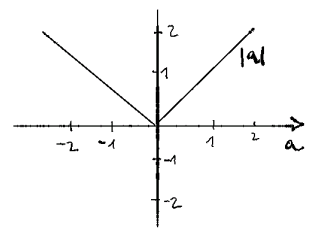
\includegraphics[width=0.4\textwidth]{betrag.png}
    \caption{Der Verlauf Funktion $f(x) =  x \, mod \, 4$.}
    \label{fig:modulo}
\end{figure}


\bgInfo{
    Formaler ist die modulo Operation definiert als:
    $$ a{\bmod {m}}:=a-\left\lfloor {\frac {a}{m}}\right\rfloor \cdot m.$$
    Wobei die sog. Gaussklammern $\lfloor \cdot \rfloor$ hier fuer 'nach unten runden' (Engl. 'truncation') stehen. 

}



% \begin{wrapfigure}{r}{0.4\textwidth}
%     \centering
%     %% Creator: Matplotlib, PGF backend
%%
%% To include the figure in your LaTeX document, write
%%   \input{<filename>.pgf}
%%
%% Make sure the required packages are loaded in your preamble
%%   \usepackage{pgf}
%%
%% Also ensure that all the required font packages are loaded; for instance,
%% the lmodern package is sometimes necessary when using math font.
%%   \usepackage{lmodern}
%%
%% Figures using additional raster images can only be included by \input if
%% they are in the same directory as the main LaTeX file. For loading figures
%% from other directories you can use the `import` package
%%   \usepackage{import}
%%
%% and then include the figures with
%%   \import{<path to file>}{<filename>.pgf}
%%
%% Matplotlib used the following preamble
%%   \def\mathdefault#1{#1}
%%   \everymath=\expandafter{\the\everymath\displaystyle}
%%   
%%   \usepackage{fontspec}
%%   \setmainfont{VeraSe.ttf}[Path=\detokenize{/usr/share/fonts/TTF/}]
%%   \setsansfont{DejaVuSans.ttf}[Path=\detokenize{/home/pl/miniconda3/lib/python3.12/site-packages/matplotlib/mpl-data/fonts/ttf/}]
%%   \setmonofont{DejaVuSansMono.ttf}[Path=\detokenize{/home/pl/miniconda3/lib/python3.12/site-packages/matplotlib/mpl-data/fonts/ttf/}]
%%   \makeatletter\@ifpackageloaded{underscore}{}{\usepackage[strings]{underscore}}\makeatother
%%
\begingroup%
\makeatletter%
\begin{pgfpicture}%
\pgfpathrectangle{\pgfpointorigin}{\pgfqpoint{2.710588in}{2.958486in}}%
\pgfusepath{use as bounding box, clip}%
\begin{pgfscope}%
\pgfsetbuttcap%
\pgfsetmiterjoin%
\definecolor{currentfill}{rgb}{1.000000,1.000000,1.000000}%
\pgfsetfillcolor{currentfill}%
\pgfsetlinewidth{0.000000pt}%
\definecolor{currentstroke}{rgb}{1.000000,1.000000,1.000000}%
\pgfsetstrokecolor{currentstroke}%
\pgfsetdash{}{0pt}%
\pgfpathmoveto{\pgfqpoint{0.000000in}{0.000000in}}%
\pgfpathlineto{\pgfqpoint{2.710588in}{0.000000in}}%
\pgfpathlineto{\pgfqpoint{2.710588in}{2.958486in}}%
\pgfpathlineto{\pgfqpoint{0.000000in}{2.958486in}}%
\pgfpathlineto{\pgfqpoint{0.000000in}{0.000000in}}%
\pgfpathclose%
\pgfusepath{fill}%
\end{pgfscope}%
\begin{pgfscope}%
\pgfsetbuttcap%
\pgfsetmiterjoin%
\definecolor{currentfill}{rgb}{1.000000,1.000000,1.000000}%
\pgfsetfillcolor{currentfill}%
\pgfsetlinewidth{0.000000pt}%
\definecolor{currentstroke}{rgb}{0.000000,0.000000,0.000000}%
\pgfsetstrokecolor{currentstroke}%
\pgfsetstrokeopacity{0.000000}%
\pgfsetdash{}{0pt}%
\pgfpathmoveto{\pgfqpoint{0.285587in}{0.548486in}}%
\pgfpathlineto{\pgfqpoint{2.610587in}{0.548486in}}%
\pgfpathlineto{\pgfqpoint{2.610587in}{2.858486in}}%
\pgfpathlineto{\pgfqpoint{0.285587in}{2.858486in}}%
\pgfpathlineto{\pgfqpoint{0.285587in}{0.548486in}}%
\pgfpathclose%
\pgfusepath{fill}%
\end{pgfscope}%
\begin{pgfscope}%
\pgfpathrectangle{\pgfqpoint{0.285587in}{0.548486in}}{\pgfqpoint{2.325000in}{2.310000in}}%
\pgfusepath{clip}%
\pgfsetrectcap%
\pgfsetroundjoin%
\pgfsetlinewidth{0.803000pt}%
\definecolor{currentstroke}{rgb}{0.690196,0.690196,0.690196}%
\pgfsetstrokecolor{currentstroke}%
\pgfsetdash{}{0pt}%
\pgfpathmoveto{\pgfqpoint{0.743542in}{0.548486in}}%
\pgfpathlineto{\pgfqpoint{0.743542in}{2.858486in}}%
\pgfusepath{stroke}%
\end{pgfscope}%
\begin{pgfscope}%
\pgfsetbuttcap%
\pgfsetroundjoin%
\definecolor{currentfill}{rgb}{0.000000,0.000000,0.000000}%
\pgfsetfillcolor{currentfill}%
\pgfsetlinewidth{0.803000pt}%
\definecolor{currentstroke}{rgb}{0.000000,0.000000,0.000000}%
\pgfsetstrokecolor{currentstroke}%
\pgfsetdash{}{0pt}%
\pgfsys@defobject{currentmarker}{\pgfqpoint{0.000000in}{-0.048611in}}{\pgfqpoint{0.000000in}{0.000000in}}{%
\pgfpathmoveto{\pgfqpoint{0.000000in}{0.000000in}}%
\pgfpathlineto{\pgfqpoint{0.000000in}{-0.048611in}}%
\pgfusepath{stroke,fill}%
}%
\begin{pgfscope}%
\pgfsys@transformshift{0.743542in}{0.548486in}%
\pgfsys@useobject{currentmarker}{}%
\end{pgfscope}%
\end{pgfscope}%
\begin{pgfscope}%
\definecolor{textcolor}{rgb}{0.000000,0.000000,0.000000}%
\pgfsetstrokecolor{textcolor}%
\pgfsetfillcolor{textcolor}%
\pgftext[x=0.743542in,y=0.451264in,,top]{\color{textcolor}{\rmfamily\fontsize{10.000000}{12.000000}\selectfont\catcode`\^=\active\def^{\ifmmode\sp\else\^{}\fi}\catcode`\%=\active\def%{\%}0}}%
\end{pgfscope}%
\begin{pgfscope}%
\pgfpathrectangle{\pgfqpoint{0.285587in}{0.548486in}}{\pgfqpoint{2.325000in}{2.310000in}}%
\pgfusepath{clip}%
\pgfsetrectcap%
\pgfsetroundjoin%
\pgfsetlinewidth{0.803000pt}%
\definecolor{currentstroke}{rgb}{0.690196,0.690196,0.690196}%
\pgfsetstrokecolor{currentstroke}%
\pgfsetdash{}{0pt}%
\pgfpathmoveto{\pgfqpoint{1.330663in}{0.548486in}}%
\pgfpathlineto{\pgfqpoint{1.330663in}{2.858486in}}%
\pgfusepath{stroke}%
\end{pgfscope}%
\begin{pgfscope}%
\pgfsetbuttcap%
\pgfsetroundjoin%
\definecolor{currentfill}{rgb}{0.000000,0.000000,0.000000}%
\pgfsetfillcolor{currentfill}%
\pgfsetlinewidth{0.803000pt}%
\definecolor{currentstroke}{rgb}{0.000000,0.000000,0.000000}%
\pgfsetstrokecolor{currentstroke}%
\pgfsetdash{}{0pt}%
\pgfsys@defobject{currentmarker}{\pgfqpoint{0.000000in}{-0.048611in}}{\pgfqpoint{0.000000in}{0.000000in}}{%
\pgfpathmoveto{\pgfqpoint{0.000000in}{0.000000in}}%
\pgfpathlineto{\pgfqpoint{0.000000in}{-0.048611in}}%
\pgfusepath{stroke,fill}%
}%
\begin{pgfscope}%
\pgfsys@transformshift{1.330663in}{0.548486in}%
\pgfsys@useobject{currentmarker}{}%
\end{pgfscope}%
\end{pgfscope}%
\begin{pgfscope}%
\definecolor{textcolor}{rgb}{0.000000,0.000000,0.000000}%
\pgfsetstrokecolor{textcolor}%
\pgfsetfillcolor{textcolor}%
\pgftext[x=1.330663in,y=0.451264in,,top]{\color{textcolor}{\rmfamily\fontsize{10.000000}{12.000000}\selectfont\catcode`\^=\active\def^{\ifmmode\sp\else\^{}\fi}\catcode`\%=\active\def%{\%}5}}%
\end{pgfscope}%
\begin{pgfscope}%
\pgfpathrectangle{\pgfqpoint{0.285587in}{0.548486in}}{\pgfqpoint{2.325000in}{2.310000in}}%
\pgfusepath{clip}%
\pgfsetrectcap%
\pgfsetroundjoin%
\pgfsetlinewidth{0.803000pt}%
\definecolor{currentstroke}{rgb}{0.690196,0.690196,0.690196}%
\pgfsetstrokecolor{currentstroke}%
\pgfsetdash{}{0pt}%
\pgfpathmoveto{\pgfqpoint{1.917784in}{0.548486in}}%
\pgfpathlineto{\pgfqpoint{1.917784in}{2.858486in}}%
\pgfusepath{stroke}%
\end{pgfscope}%
\begin{pgfscope}%
\pgfsetbuttcap%
\pgfsetroundjoin%
\definecolor{currentfill}{rgb}{0.000000,0.000000,0.000000}%
\pgfsetfillcolor{currentfill}%
\pgfsetlinewidth{0.803000pt}%
\definecolor{currentstroke}{rgb}{0.000000,0.000000,0.000000}%
\pgfsetstrokecolor{currentstroke}%
\pgfsetdash{}{0pt}%
\pgfsys@defobject{currentmarker}{\pgfqpoint{0.000000in}{-0.048611in}}{\pgfqpoint{0.000000in}{0.000000in}}{%
\pgfpathmoveto{\pgfqpoint{0.000000in}{0.000000in}}%
\pgfpathlineto{\pgfqpoint{0.000000in}{-0.048611in}}%
\pgfusepath{stroke,fill}%
}%
\begin{pgfscope}%
\pgfsys@transformshift{1.917784in}{0.548486in}%
\pgfsys@useobject{currentmarker}{}%
\end{pgfscope}%
\end{pgfscope}%
\begin{pgfscope}%
\definecolor{textcolor}{rgb}{0.000000,0.000000,0.000000}%
\pgfsetstrokecolor{textcolor}%
\pgfsetfillcolor{textcolor}%
\pgftext[x=1.917784in,y=0.451264in,,top]{\color{textcolor}{\rmfamily\fontsize{10.000000}{12.000000}\selectfont\catcode`\^=\active\def^{\ifmmode\sp\else\^{}\fi}\catcode`\%=\active\def%{\%}10}}%
\end{pgfscope}%
\begin{pgfscope}%
\pgfpathrectangle{\pgfqpoint{0.285587in}{0.548486in}}{\pgfqpoint{2.325000in}{2.310000in}}%
\pgfusepath{clip}%
\pgfsetrectcap%
\pgfsetroundjoin%
\pgfsetlinewidth{0.803000pt}%
\definecolor{currentstroke}{rgb}{0.690196,0.690196,0.690196}%
\pgfsetstrokecolor{currentstroke}%
\pgfsetdash{}{0pt}%
\pgfpathmoveto{\pgfqpoint{2.504906in}{0.548486in}}%
\pgfpathlineto{\pgfqpoint{2.504906in}{2.858486in}}%
\pgfusepath{stroke}%
\end{pgfscope}%
\begin{pgfscope}%
\pgfsetbuttcap%
\pgfsetroundjoin%
\definecolor{currentfill}{rgb}{0.000000,0.000000,0.000000}%
\pgfsetfillcolor{currentfill}%
\pgfsetlinewidth{0.803000pt}%
\definecolor{currentstroke}{rgb}{0.000000,0.000000,0.000000}%
\pgfsetstrokecolor{currentstroke}%
\pgfsetdash{}{0pt}%
\pgfsys@defobject{currentmarker}{\pgfqpoint{0.000000in}{-0.048611in}}{\pgfqpoint{0.000000in}{0.000000in}}{%
\pgfpathmoveto{\pgfqpoint{0.000000in}{0.000000in}}%
\pgfpathlineto{\pgfqpoint{0.000000in}{-0.048611in}}%
\pgfusepath{stroke,fill}%
}%
\begin{pgfscope}%
\pgfsys@transformshift{2.504906in}{0.548486in}%
\pgfsys@useobject{currentmarker}{}%
\end{pgfscope}%
\end{pgfscope}%
\begin{pgfscope}%
\definecolor{textcolor}{rgb}{0.000000,0.000000,0.000000}%
\pgfsetstrokecolor{textcolor}%
\pgfsetfillcolor{textcolor}%
\pgftext[x=2.504906in,y=0.451264in,,top]{\color{textcolor}{\rmfamily\fontsize{10.000000}{12.000000}\selectfont\catcode`\^=\active\def^{\ifmmode\sp\else\^{}\fi}\catcode`\%=\active\def%{\%}15}}%
\end{pgfscope}%
\begin{pgfscope}%
\definecolor{textcolor}{rgb}{0.000000,0.000000,0.000000}%
\pgfsetstrokecolor{textcolor}%
\pgfsetfillcolor{textcolor}%
\pgftext[x=1.448087in,y=0.261295in,,top]{\color{textcolor}{\rmfamily\fontsize{12.000000}{14.400000}\selectfont\catcode`\^=\active\def^{\ifmmode\sp\else\^{}\fi}\catcode`\%=\active\def%{\%}$x$}}%
\end{pgfscope}%
\begin{pgfscope}%
\pgfpathrectangle{\pgfqpoint{0.285587in}{0.548486in}}{\pgfqpoint{2.325000in}{2.310000in}}%
\pgfusepath{clip}%
\pgfsetrectcap%
\pgfsetroundjoin%
\pgfsetlinewidth{0.803000pt}%
\definecolor{currentstroke}{rgb}{0.690196,0.690196,0.690196}%
\pgfsetstrokecolor{currentstroke}%
\pgfsetdash{}{0pt}%
\pgfpathmoveto{\pgfqpoint{0.285587in}{0.648735in}}%
\pgfpathlineto{\pgfqpoint{2.610587in}{0.648735in}}%
\pgfusepath{stroke}%
\end{pgfscope}%
\begin{pgfscope}%
\pgfsetbuttcap%
\pgfsetroundjoin%
\definecolor{currentfill}{rgb}{0.000000,0.000000,0.000000}%
\pgfsetfillcolor{currentfill}%
\pgfsetlinewidth{0.803000pt}%
\definecolor{currentstroke}{rgb}{0.000000,0.000000,0.000000}%
\pgfsetstrokecolor{currentstroke}%
\pgfsetdash{}{0pt}%
\pgfsys@defobject{currentmarker}{\pgfqpoint{-0.048611in}{0.000000in}}{\pgfqpoint{-0.000000in}{0.000000in}}{%
\pgfpathmoveto{\pgfqpoint{-0.000000in}{0.000000in}}%
\pgfpathlineto{\pgfqpoint{-0.048611in}{0.000000in}}%
\pgfusepath{stroke,fill}%
}%
\begin{pgfscope}%
\pgfsys@transformshift{0.285587in}{0.648735in}%
\pgfsys@useobject{currentmarker}{}%
\end{pgfscope}%
\end{pgfscope}%
\begin{pgfscope}%
\definecolor{textcolor}{rgb}{0.000000,0.000000,0.000000}%
\pgfsetstrokecolor{textcolor}%
\pgfsetfillcolor{textcolor}%
\pgftext[x=0.100000in, y=0.595973in, left, base]{\color{textcolor}{\rmfamily\fontsize{10.000000}{12.000000}\selectfont\catcode`\^=\active\def^{\ifmmode\sp\else\^{}\fi}\catcode`\%=\active\def%{\%}0}}%
\end{pgfscope}%
\begin{pgfscope}%
\pgfpathrectangle{\pgfqpoint{0.285587in}{0.548486in}}{\pgfqpoint{2.325000in}{2.310000in}}%
\pgfusepath{clip}%
\pgfsetrectcap%
\pgfsetroundjoin%
\pgfsetlinewidth{0.803000pt}%
\definecolor{currentstroke}{rgb}{0.690196,0.690196,0.690196}%
\pgfsetstrokecolor{currentstroke}%
\pgfsetdash{}{0pt}%
\pgfpathmoveto{\pgfqpoint{0.285587in}{1.176110in}}%
\pgfpathlineto{\pgfqpoint{2.610587in}{1.176110in}}%
\pgfusepath{stroke}%
\end{pgfscope}%
\begin{pgfscope}%
\pgfsetbuttcap%
\pgfsetroundjoin%
\definecolor{currentfill}{rgb}{0.000000,0.000000,0.000000}%
\pgfsetfillcolor{currentfill}%
\pgfsetlinewidth{0.803000pt}%
\definecolor{currentstroke}{rgb}{0.000000,0.000000,0.000000}%
\pgfsetstrokecolor{currentstroke}%
\pgfsetdash{}{0pt}%
\pgfsys@defobject{currentmarker}{\pgfqpoint{-0.048611in}{0.000000in}}{\pgfqpoint{-0.000000in}{0.000000in}}{%
\pgfpathmoveto{\pgfqpoint{-0.000000in}{0.000000in}}%
\pgfpathlineto{\pgfqpoint{-0.048611in}{0.000000in}}%
\pgfusepath{stroke,fill}%
}%
\begin{pgfscope}%
\pgfsys@transformshift{0.285587in}{1.176110in}%
\pgfsys@useobject{currentmarker}{}%
\end{pgfscope}%
\end{pgfscope}%
\begin{pgfscope}%
\definecolor{textcolor}{rgb}{0.000000,0.000000,0.000000}%
\pgfsetstrokecolor{textcolor}%
\pgfsetfillcolor{textcolor}%
\pgftext[x=0.100000in, y=1.123349in, left, base]{\color{textcolor}{\rmfamily\fontsize{10.000000}{12.000000}\selectfont\catcode`\^=\active\def^{\ifmmode\sp\else\^{}\fi}\catcode`\%=\active\def%{\%}1}}%
\end{pgfscope}%
\begin{pgfscope}%
\pgfpathrectangle{\pgfqpoint{0.285587in}{0.548486in}}{\pgfqpoint{2.325000in}{2.310000in}}%
\pgfusepath{clip}%
\pgfsetrectcap%
\pgfsetroundjoin%
\pgfsetlinewidth{0.803000pt}%
\definecolor{currentstroke}{rgb}{0.690196,0.690196,0.690196}%
\pgfsetstrokecolor{currentstroke}%
\pgfsetdash{}{0pt}%
\pgfpathmoveto{\pgfqpoint{0.285587in}{1.703486in}}%
\pgfpathlineto{\pgfqpoint{2.610587in}{1.703486in}}%
\pgfusepath{stroke}%
\end{pgfscope}%
\begin{pgfscope}%
\pgfsetbuttcap%
\pgfsetroundjoin%
\definecolor{currentfill}{rgb}{0.000000,0.000000,0.000000}%
\pgfsetfillcolor{currentfill}%
\pgfsetlinewidth{0.803000pt}%
\definecolor{currentstroke}{rgb}{0.000000,0.000000,0.000000}%
\pgfsetstrokecolor{currentstroke}%
\pgfsetdash{}{0pt}%
\pgfsys@defobject{currentmarker}{\pgfqpoint{-0.048611in}{0.000000in}}{\pgfqpoint{-0.000000in}{0.000000in}}{%
\pgfpathmoveto{\pgfqpoint{-0.000000in}{0.000000in}}%
\pgfpathlineto{\pgfqpoint{-0.048611in}{0.000000in}}%
\pgfusepath{stroke,fill}%
}%
\begin{pgfscope}%
\pgfsys@transformshift{0.285587in}{1.703486in}%
\pgfsys@useobject{currentmarker}{}%
\end{pgfscope}%
\end{pgfscope}%
\begin{pgfscope}%
\definecolor{textcolor}{rgb}{0.000000,0.000000,0.000000}%
\pgfsetstrokecolor{textcolor}%
\pgfsetfillcolor{textcolor}%
\pgftext[x=0.100000in, y=1.650724in, left, base]{\color{textcolor}{\rmfamily\fontsize{10.000000}{12.000000}\selectfont\catcode`\^=\active\def^{\ifmmode\sp\else\^{}\fi}\catcode`\%=\active\def%{\%}2}}%
\end{pgfscope}%
\begin{pgfscope}%
\pgfpathrectangle{\pgfqpoint{0.285587in}{0.548486in}}{\pgfqpoint{2.325000in}{2.310000in}}%
\pgfusepath{clip}%
\pgfsetrectcap%
\pgfsetroundjoin%
\pgfsetlinewidth{0.803000pt}%
\definecolor{currentstroke}{rgb}{0.690196,0.690196,0.690196}%
\pgfsetstrokecolor{currentstroke}%
\pgfsetdash{}{0pt}%
\pgfpathmoveto{\pgfqpoint{0.285587in}{2.230862in}}%
\pgfpathlineto{\pgfqpoint{2.610587in}{2.230862in}}%
\pgfusepath{stroke}%
\end{pgfscope}%
\begin{pgfscope}%
\pgfsetbuttcap%
\pgfsetroundjoin%
\definecolor{currentfill}{rgb}{0.000000,0.000000,0.000000}%
\pgfsetfillcolor{currentfill}%
\pgfsetlinewidth{0.803000pt}%
\definecolor{currentstroke}{rgb}{0.000000,0.000000,0.000000}%
\pgfsetstrokecolor{currentstroke}%
\pgfsetdash{}{0pt}%
\pgfsys@defobject{currentmarker}{\pgfqpoint{-0.048611in}{0.000000in}}{\pgfqpoint{-0.000000in}{0.000000in}}{%
\pgfpathmoveto{\pgfqpoint{-0.000000in}{0.000000in}}%
\pgfpathlineto{\pgfqpoint{-0.048611in}{0.000000in}}%
\pgfusepath{stroke,fill}%
}%
\begin{pgfscope}%
\pgfsys@transformshift{0.285587in}{2.230862in}%
\pgfsys@useobject{currentmarker}{}%
\end{pgfscope}%
\end{pgfscope}%
\begin{pgfscope}%
\definecolor{textcolor}{rgb}{0.000000,0.000000,0.000000}%
\pgfsetstrokecolor{textcolor}%
\pgfsetfillcolor{textcolor}%
\pgftext[x=0.100000in, y=2.178100in, left, base]{\color{textcolor}{\rmfamily\fontsize{10.000000}{12.000000}\selectfont\catcode`\^=\active\def^{\ifmmode\sp\else\^{}\fi}\catcode`\%=\active\def%{\%}3}}%
\end{pgfscope}%
\begin{pgfscope}%
\pgfpathrectangle{\pgfqpoint{0.285587in}{0.548486in}}{\pgfqpoint{2.325000in}{2.310000in}}%
\pgfusepath{clip}%
\pgfsetrectcap%
\pgfsetroundjoin%
\pgfsetlinewidth{0.803000pt}%
\definecolor{currentstroke}{rgb}{0.690196,0.690196,0.690196}%
\pgfsetstrokecolor{currentstroke}%
\pgfsetdash{}{0pt}%
\pgfpathmoveto{\pgfqpoint{0.285587in}{2.758237in}}%
\pgfpathlineto{\pgfqpoint{2.610587in}{2.758237in}}%
\pgfusepath{stroke}%
\end{pgfscope}%
\begin{pgfscope}%
\pgfsetbuttcap%
\pgfsetroundjoin%
\definecolor{currentfill}{rgb}{0.000000,0.000000,0.000000}%
\pgfsetfillcolor{currentfill}%
\pgfsetlinewidth{0.803000pt}%
\definecolor{currentstroke}{rgb}{0.000000,0.000000,0.000000}%
\pgfsetstrokecolor{currentstroke}%
\pgfsetdash{}{0pt}%
\pgfsys@defobject{currentmarker}{\pgfqpoint{-0.048611in}{0.000000in}}{\pgfqpoint{-0.000000in}{0.000000in}}{%
\pgfpathmoveto{\pgfqpoint{-0.000000in}{0.000000in}}%
\pgfpathlineto{\pgfqpoint{-0.048611in}{0.000000in}}%
\pgfusepath{stroke,fill}%
}%
\begin{pgfscope}%
\pgfsys@transformshift{0.285587in}{2.758237in}%
\pgfsys@useobject{currentmarker}{}%
\end{pgfscope}%
\end{pgfscope}%
\begin{pgfscope}%
\definecolor{textcolor}{rgb}{0.000000,0.000000,0.000000}%
\pgfsetstrokecolor{textcolor}%
\pgfsetfillcolor{textcolor}%
\pgftext[x=0.100000in, y=2.705476in, left, base]{\color{textcolor}{\rmfamily\fontsize{10.000000}{12.000000}\selectfont\catcode`\^=\active\def^{\ifmmode\sp\else\^{}\fi}\catcode`\%=\active\def%{\%}4}}%
\end{pgfscope}%
\begin{pgfscope}%
\pgfpathrectangle{\pgfqpoint{0.285587in}{0.548486in}}{\pgfqpoint{2.325000in}{2.310000in}}%
\pgfusepath{clip}%
\pgfsetrectcap%
\pgfsetroundjoin%
\pgfsetlinewidth{1.505625pt}%
\definecolor{currentstroke}{rgb}{0.000000,0.000000,0.000000}%
\pgfsetstrokecolor{currentstroke}%
\pgfsetdash{}{0pt}%
\pgfpathmoveto{\pgfqpoint{0.391269in}{1.176110in}}%
\pgfpathlineto{\pgfqpoint{0.742484in}{2.753486in}}%
\pgfpathlineto{\pgfqpoint{0.744600in}{0.653486in}}%
\pgfpathlineto{\pgfqpoint{1.212181in}{2.753486in}}%
\pgfpathlineto{\pgfqpoint{1.214297in}{0.653486in}}%
\pgfpathlineto{\pgfqpoint{1.681878in}{2.753486in}}%
\pgfpathlineto{\pgfqpoint{1.683994in}{0.653486in}}%
\pgfpathlineto{\pgfqpoint{2.151575in}{2.753486in}}%
\pgfpathlineto{\pgfqpoint{2.153691in}{0.653486in}}%
\pgfpathlineto{\pgfqpoint{2.504906in}{2.230862in}}%
\pgfpathlineto{\pgfqpoint{2.504906in}{2.230862in}}%
\pgfusepath{stroke}%
\end{pgfscope}%
\begin{pgfscope}%
\pgfpathrectangle{\pgfqpoint{0.285587in}{0.548486in}}{\pgfqpoint{2.325000in}{2.310000in}}%
\pgfusepath{clip}%
\pgfsetrectcap%
\pgfsetroundjoin%
\pgfsetlinewidth{0.501875pt}%
\definecolor{currentstroke}{rgb}{0.000000,0.000000,0.000000}%
\pgfsetstrokecolor{currentstroke}%
\pgfsetdash{}{0pt}%
\pgfpathmoveto{\pgfqpoint{0.285587in}{0.648735in}}%
\pgfpathlineto{\pgfqpoint{2.610587in}{0.648735in}}%
\pgfusepath{stroke}%
\end{pgfscope}%
\begin{pgfscope}%
\pgfpathrectangle{\pgfqpoint{0.285587in}{0.548486in}}{\pgfqpoint{2.325000in}{2.310000in}}%
\pgfusepath{clip}%
\pgfsetrectcap%
\pgfsetroundjoin%
\pgfsetlinewidth{0.501875pt}%
\definecolor{currentstroke}{rgb}{0.000000,0.000000,0.000000}%
\pgfsetstrokecolor{currentstroke}%
\pgfsetdash{}{0pt}%
\pgfpathmoveto{\pgfqpoint{0.743542in}{0.548486in}}%
\pgfpathlineto{\pgfqpoint{0.743542in}{2.858486in}}%
\pgfusepath{stroke}%
\end{pgfscope}%
\end{pgfpicture}%
\makeatother%
\endgroup%

%     \caption{An example figure}
% \end{wrapfigure}

\subsection{Summe und Produkt Notation}

Das große Sigma, $\Sigma$ ist eine kurzschreibweise für Summen. Wir finden dieses Zeichen oft in Blockdiagrammen um eine Addition zu verdeutlichen und manchmal sogar auf Mischpulten als Zier in der Gegend der 'Summe'/des Master Faders. Es handelt sich um eine simple Addition, also nichts was zu Irritation führen sollte. In der Praxis kann es allerdings vorkommen dass, sich vor allem bei unendlichen Summen einige Komplexität hinter so einer Summer verbirgt. Die Notation alleine sollte aber nicht abschrecken:

\begin{equation}
{\displaystyle \sum _{k=1}^{5}k = 1 + 2 + 3 + 4 + 5 }
\end{equation}
\emph{Index}
Hier ist $k$ der Index (Auch 'Laufindex' oder 'Zähler' genannt). Unter dem Sigma steht bei welcher zahl zu zählen begonnen wird und welchen Buchstaben wir als Index wählen. über dem Sigma steht bis wohin wir zählen. Nach dem Sigma steht was addiert wird. Allgemein:

\important{
\begin{equation}
{\displaystyle \sum _{k=m}^{n}a_{k}=\sum _{m\leq k\leq n}a_{k}=a_{m}+a_{m+1}+\dotsb +a_{n}.}
\end{equation}
}


Natürlich kann diese Schreibweise verwendet werden um kompliziertere Ausdrücke zu formen.

\begin{question}
Schreiben Sie einen Ausdruck der die \textbf{geraden} Zahlen zwischen 0 und 11 quadriert und addiert!
\end{question}
\begin{answer}

$${\displaystyle \sum _{k=0}^{5} (k \cdot 2)^2 = 0 + (1 \cdot 2)^2 + (2 \cdot 2)^2 + (3 \cdot 2)^2 + (4 \cdot 2)^2 + (5 \cdot 2)^2}$$

\end{answer}


\praxis{Im Audio Bereich finden wir Summenzeichen in vielen Bereichen. Bei der Diskreten Fourier Transformation, bei Filtern, bei der Beschreibung des Zusammenmischens vieler Signale im Allgemeinen (egal ob elektrisch oder akustisch), bei 'Discrete Summation Formula'(DSF)-Synthese und in vielen anderen Bereichen.}


% \todo[]{summe erklärungen, beispiel. Praxisbezug. Beschreibung des ausgangssignals bei einem Mixer, DSF synthesis, diskrete fourier transf. }

% \todo[]{prod. Beispiel filter Kaskadieren (produkte)}

Die Notation für Produkte trifft man nicht ganz so oft an wie jene für Summen:

\begin{equation}
{\displaystyle \prod _{i=1}^{6}i^{2} =  1\cdot 4\cdot 9\cdot 16\cdot 25\cdot 36}
\end{equation}

Im Audio Bereich ist natürlich auch diese Notation wichtig (Multiplikation ist eine wichtige Operation). Ein Beispiel wäre, gegeben einen Filter mit der Transferfunktion $H$ könnte man $n$ hintereinander geschaltene ('kaskadierte') Filter schreiben als $\prod _{i=1}^{n}H$.


\subsection{Betrag}

% \begin{wrapfigure}{r}{0.4\textwidth}
%     \centering
%     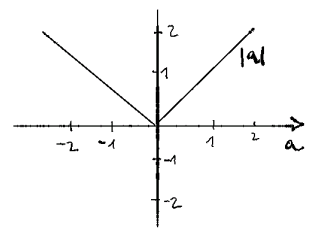
\includegraphics[width=0.4\textwidth]{betrag.png}
%     \caption{Betrag als Input/Output Plot.}
%     \label{fig:betrag}
% \end{wrapfigure}

Der Betrag macht alles positiv. Der \emph{Betrag} einer Zahl $a \in \mathbb{R}$, dargestellt als $|a|$ kann folgendermaßen definiert werden:
$$ 
|a| \coloneqq
\begin{cases} 
-a & \text{wenn } a < 0 \\ 
a & \text{wenn } a \geq 0 
\end{cases}
$$ 

Der Betrag kann als \emph{Funktion} aufgefasst werden (später mehr zu Funktionen). Es Kann ein Graph gezeichnet werden auf dessen x-Achse ('Abszisse') der Input zu sehen ist und auf der y-Achse ('Ordinate'). 
\bgInfo{Merkhilfe: Alphabetisch, x vor y, Abszisse vor Ordinate.}



\begin{figure}[h!]
    \centering
    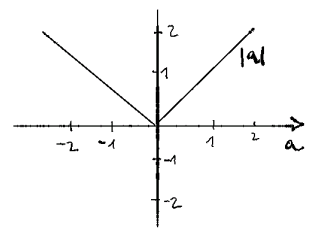
\includegraphics[width=0.4\textwidth]{betrag.png}
    \caption{Betrag als Input/Output Plot.}
    \label{fig:betrag}
\end{figure}

\index{Betrag}
\index{Absolutwert}

\praxis{
Der Betrag (oder auch Absolutwert) hat in der Audio Technik eine Wichtige Rolle, speziell der Betrag von Komplexen Zahlen, den Ergebnissen der Fourier Transformation. In der Elektrotechnik kann er als 'Gleichrichter' gefunden werden um Wechselströme zu Gleichströmen zu wandeln. Er ist eine der simpelsten Verzerrungen mit geraden harmonischen.
}

Soundbeispiel hier: \faust{Betrag Einer 150Hz Sinus Schwingung}{https://faustide.grame.fr/?autorun=1\&voices=0\&name=abs_test\&inline=aW1wb3J0KCJzdGRmYXVzdC5saWIiKTsKcHJvY2VzcyA9IG9zLm9zYygxNTApOmFiczs\%3D}

\begin{figure}[H]
    \centering
    %% Creator: Matplotlib, PGF backend
%%
%% To include the figure in your LaTeX document, write
%%   \input{<filename>.pgf}
%%
%% Make sure the required packages are loaded in your preamble
%%   \usepackage{pgf}
%%
%% Also ensure that all the required font packages are loaded; for instance,
%% the lmodern package is sometimes necessary when using math font.
%%   \usepackage{lmodern}
%%
%% Figures using additional raster images can only be included by \input if
%% they are in the same directory as the main LaTeX file. For loading figures
%% from other directories you can use the `import` package
%%   \usepackage{import}
%%
%% and then include the figures with
%%   \import{<path to file>}{<filename>.pgf}
%%
%% Matplotlib used the following preamble
%%   \def\mathdefault#1{#1}
%%   \everymath=\expandafter{\the\everymath\displaystyle}
%%   
%%   \usepackage{fontspec}
%%   \setmainfont{VeraSe.ttf}[Path=\detokenize{/usr/share/fonts/TTF/}]
%%   \setsansfont{DejaVuSans.ttf}[Path=\detokenize{/home/pl/miniconda3/lib/python3.12/site-packages/matplotlib/mpl-data/fonts/ttf/}]
%%   \setmonofont{DejaVuSansMono.ttf}[Path=\detokenize{/home/pl/miniconda3/lib/python3.12/site-packages/matplotlib/mpl-data/fonts/ttf/}]
%%   \makeatletter\@ifpackageloaded{underscore}{}{\usepackage[strings]{underscore}}\makeatother
%%
\begingroup%
\makeatletter%
\begin{pgfpicture}%
\pgfpathrectangle{\pgfpointorigin}{\pgfqpoint{5.276127in}{1.740000in}}%
\pgfusepath{use as bounding box, clip}%
\begin{pgfscope}%
\pgfsetbuttcap%
\pgfsetmiterjoin%
\definecolor{currentfill}{rgb}{1.000000,1.000000,1.000000}%
\pgfsetfillcolor{currentfill}%
\pgfsetlinewidth{0.000000pt}%
\definecolor{currentstroke}{rgb}{1.000000,1.000000,1.000000}%
\pgfsetstrokecolor{currentstroke}%
\pgfsetdash{}{0pt}%
\pgfpathmoveto{\pgfqpoint{0.000000in}{0.000000in}}%
\pgfpathlineto{\pgfqpoint{5.276127in}{0.000000in}}%
\pgfpathlineto{\pgfqpoint{5.276127in}{1.740000in}}%
\pgfpathlineto{\pgfqpoint{0.000000in}{1.740000in}}%
\pgfpathlineto{\pgfqpoint{0.000000in}{0.000000in}}%
\pgfpathclose%
\pgfusepath{fill}%
\end{pgfscope}%
\begin{pgfscope}%
\pgfsetbuttcap%
\pgfsetmiterjoin%
\definecolor{currentfill}{rgb}{1.000000,1.000000,1.000000}%
\pgfsetfillcolor{currentfill}%
\pgfsetlinewidth{0.000000pt}%
\definecolor{currentstroke}{rgb}{0.000000,0.000000,0.000000}%
\pgfsetstrokecolor{currentstroke}%
\pgfsetstrokeopacity{0.000000}%
\pgfsetdash{}{0pt}%
\pgfpathmoveto{\pgfqpoint{0.526127in}{0.100000in}}%
\pgfpathlineto{\pgfqpoint{2.639763in}{0.100000in}}%
\pgfpathlineto{\pgfqpoint{2.639763in}{1.640000in}}%
\pgfpathlineto{\pgfqpoint{0.526127in}{1.640000in}}%
\pgfpathlineto{\pgfqpoint{0.526127in}{0.100000in}}%
\pgfpathclose%
\pgfusepath{fill}%
\end{pgfscope}%
\begin{pgfscope}%
\pgfsetbuttcap%
\pgfsetroundjoin%
\definecolor{currentfill}{rgb}{0.000000,0.000000,0.000000}%
\pgfsetfillcolor{currentfill}%
\pgfsetlinewidth{0.803000pt}%
\definecolor{currentstroke}{rgb}{0.000000,0.000000,0.000000}%
\pgfsetstrokecolor{currentstroke}%
\pgfsetdash{}{0pt}%
\pgfsys@defobject{currentmarker}{\pgfqpoint{-0.048611in}{0.000000in}}{\pgfqpoint{-0.000000in}{0.000000in}}{%
\pgfpathmoveto{\pgfqpoint{-0.000000in}{0.000000in}}%
\pgfpathlineto{\pgfqpoint{-0.048611in}{0.000000in}}%
\pgfusepath{stroke,fill}%
}%
\begin{pgfscope}%
\pgfsys@transformshift{0.526127in}{0.228333in}%
\pgfsys@useobject{currentmarker}{}%
\end{pgfscope}%
\end{pgfscope}%
\begin{pgfscope}%
\definecolor{textcolor}{rgb}{0.000000,0.000000,0.000000}%
\pgfsetstrokecolor{textcolor}%
\pgfsetfillcolor{textcolor}%
\pgftext[x=0.100000in, y=0.175572in, left, base]{\color{textcolor}{\rmfamily\fontsize{10.000000}{12.000000}\selectfont\catcode`\^=\active\def^{\ifmmode\sp\else\^{}\fi}\catcode`\%=\active\def%{\%}\ensuremath{-}1.0}}%
\end{pgfscope}%
\begin{pgfscope}%
\pgfsetbuttcap%
\pgfsetroundjoin%
\definecolor{currentfill}{rgb}{0.000000,0.000000,0.000000}%
\pgfsetfillcolor{currentfill}%
\pgfsetlinewidth{0.803000pt}%
\definecolor{currentstroke}{rgb}{0.000000,0.000000,0.000000}%
\pgfsetstrokecolor{currentstroke}%
\pgfsetdash{}{0pt}%
\pgfsys@defobject{currentmarker}{\pgfqpoint{-0.048611in}{0.000000in}}{\pgfqpoint{-0.000000in}{0.000000in}}{%
\pgfpathmoveto{\pgfqpoint{-0.000000in}{0.000000in}}%
\pgfpathlineto{\pgfqpoint{-0.048611in}{0.000000in}}%
\pgfusepath{stroke,fill}%
}%
\begin{pgfscope}%
\pgfsys@transformshift{0.526127in}{0.549167in}%
\pgfsys@useobject{currentmarker}{}%
\end{pgfscope}%
\end{pgfscope}%
\begin{pgfscope}%
\definecolor{textcolor}{rgb}{0.000000,0.000000,0.000000}%
\pgfsetstrokecolor{textcolor}%
\pgfsetfillcolor{textcolor}%
\pgftext[x=0.100000in, y=0.496405in, left, base]{\color{textcolor}{\rmfamily\fontsize{10.000000}{12.000000}\selectfont\catcode`\^=\active\def^{\ifmmode\sp\else\^{}\fi}\catcode`\%=\active\def%{\%}\ensuremath{-}0.5}}%
\end{pgfscope}%
\begin{pgfscope}%
\pgfsetbuttcap%
\pgfsetroundjoin%
\definecolor{currentfill}{rgb}{0.000000,0.000000,0.000000}%
\pgfsetfillcolor{currentfill}%
\pgfsetlinewidth{0.803000pt}%
\definecolor{currentstroke}{rgb}{0.000000,0.000000,0.000000}%
\pgfsetstrokecolor{currentstroke}%
\pgfsetdash{}{0pt}%
\pgfsys@defobject{currentmarker}{\pgfqpoint{-0.048611in}{0.000000in}}{\pgfqpoint{-0.000000in}{0.000000in}}{%
\pgfpathmoveto{\pgfqpoint{-0.000000in}{0.000000in}}%
\pgfpathlineto{\pgfqpoint{-0.048611in}{0.000000in}}%
\pgfusepath{stroke,fill}%
}%
\begin{pgfscope}%
\pgfsys@transformshift{0.526127in}{0.870000in}%
\pgfsys@useobject{currentmarker}{}%
\end{pgfscope}%
\end{pgfscope}%
\begin{pgfscope}%
\definecolor{textcolor}{rgb}{0.000000,0.000000,0.000000}%
\pgfsetstrokecolor{textcolor}%
\pgfsetfillcolor{textcolor}%
\pgftext[x=0.208025in, y=0.817238in, left, base]{\color{textcolor}{\rmfamily\fontsize{10.000000}{12.000000}\selectfont\catcode`\^=\active\def^{\ifmmode\sp\else\^{}\fi}\catcode`\%=\active\def%{\%}0.0}}%
\end{pgfscope}%
\begin{pgfscope}%
\pgfsetbuttcap%
\pgfsetroundjoin%
\definecolor{currentfill}{rgb}{0.000000,0.000000,0.000000}%
\pgfsetfillcolor{currentfill}%
\pgfsetlinewidth{0.803000pt}%
\definecolor{currentstroke}{rgb}{0.000000,0.000000,0.000000}%
\pgfsetstrokecolor{currentstroke}%
\pgfsetdash{}{0pt}%
\pgfsys@defobject{currentmarker}{\pgfqpoint{-0.048611in}{0.000000in}}{\pgfqpoint{-0.000000in}{0.000000in}}{%
\pgfpathmoveto{\pgfqpoint{-0.000000in}{0.000000in}}%
\pgfpathlineto{\pgfqpoint{-0.048611in}{0.000000in}}%
\pgfusepath{stroke,fill}%
}%
\begin{pgfscope}%
\pgfsys@transformshift{0.526127in}{1.190833in}%
\pgfsys@useobject{currentmarker}{}%
\end{pgfscope}%
\end{pgfscope}%
\begin{pgfscope}%
\definecolor{textcolor}{rgb}{0.000000,0.000000,0.000000}%
\pgfsetstrokecolor{textcolor}%
\pgfsetfillcolor{textcolor}%
\pgftext[x=0.208025in, y=1.138072in, left, base]{\color{textcolor}{\rmfamily\fontsize{10.000000}{12.000000}\selectfont\catcode`\^=\active\def^{\ifmmode\sp\else\^{}\fi}\catcode`\%=\active\def%{\%}0.5}}%
\end{pgfscope}%
\begin{pgfscope}%
\pgfsetbuttcap%
\pgfsetroundjoin%
\definecolor{currentfill}{rgb}{0.000000,0.000000,0.000000}%
\pgfsetfillcolor{currentfill}%
\pgfsetlinewidth{0.803000pt}%
\definecolor{currentstroke}{rgb}{0.000000,0.000000,0.000000}%
\pgfsetstrokecolor{currentstroke}%
\pgfsetdash{}{0pt}%
\pgfsys@defobject{currentmarker}{\pgfqpoint{-0.048611in}{0.000000in}}{\pgfqpoint{-0.000000in}{0.000000in}}{%
\pgfpathmoveto{\pgfqpoint{-0.000000in}{0.000000in}}%
\pgfpathlineto{\pgfqpoint{-0.048611in}{0.000000in}}%
\pgfusepath{stroke,fill}%
}%
\begin{pgfscope}%
\pgfsys@transformshift{0.526127in}{1.511667in}%
\pgfsys@useobject{currentmarker}{}%
\end{pgfscope}%
\end{pgfscope}%
\begin{pgfscope}%
\definecolor{textcolor}{rgb}{0.000000,0.000000,0.000000}%
\pgfsetstrokecolor{textcolor}%
\pgfsetfillcolor{textcolor}%
\pgftext[x=0.208025in, y=1.458905in, left, base]{\color{textcolor}{\rmfamily\fontsize{10.000000}{12.000000}\selectfont\catcode`\^=\active\def^{\ifmmode\sp\else\^{}\fi}\catcode`\%=\active\def%{\%}1.0}}%
\end{pgfscope}%
\begin{pgfscope}%
\pgfpathrectangle{\pgfqpoint{0.526127in}{0.100000in}}{\pgfqpoint{2.113636in}{1.540000in}}%
\pgfusepath{clip}%
\pgfsetrectcap%
\pgfsetroundjoin%
\pgfsetlinewidth{1.505625pt}%
\definecolor{currentstroke}{rgb}{0.000000,0.000000,0.000000}%
\pgfsetstrokecolor{currentstroke}%
\pgfsetdash{}{0pt}%
\pgfpathmoveto{\pgfqpoint{0.622201in}{0.870000in}}%
\pgfpathlineto{\pgfqpoint{0.717208in}{0.968077in}}%
\pgfpathlineto{\pgfqpoint{0.767762in}{1.017008in}}%
\pgfpathlineto{\pgfqpoint{0.810035in}{1.054901in}}%
\pgfpathlineto{\pgfqpoint{0.847515in}{1.085567in}}%
\pgfpathlineto{\pgfqpoint{0.881944in}{1.110898in}}%
\pgfpathlineto{\pgfqpoint{0.913758in}{1.131600in}}%
\pgfpathlineto{\pgfqpoint{0.943829in}{1.148571in}}%
\pgfpathlineto{\pgfqpoint{0.972593in}{1.162288in}}%
\pgfpathlineto{\pgfqpoint{1.000049in}{1.172972in}}%
\pgfpathlineto{\pgfqpoint{1.027069in}{1.181104in}}%
\pgfpathlineto{\pgfqpoint{1.053217in}{1.186664in}}%
\pgfpathlineto{\pgfqpoint{1.078930in}{1.189875in}}%
\pgfpathlineto{\pgfqpoint{1.104643in}{1.190826in}}%
\pgfpathlineto{\pgfqpoint{1.129920in}{1.189551in}}%
\pgfpathlineto{\pgfqpoint{1.155633in}{1.186016in}}%
\pgfpathlineto{\pgfqpoint{1.181346in}{1.180249in}}%
\pgfpathlineto{\pgfqpoint{1.207930in}{1.171981in}}%
\pgfpathlineto{\pgfqpoint{1.234950in}{1.161242in}}%
\pgfpathlineto{\pgfqpoint{1.263278in}{1.147545in}}%
\pgfpathlineto{\pgfqpoint{1.292477in}{1.130937in}}%
\pgfpathlineto{\pgfqpoint{1.323420in}{1.110747in}}%
\pgfpathlineto{\pgfqpoint{1.356541in}{1.086412in}}%
\pgfpathlineto{\pgfqpoint{1.392278in}{1.057321in}}%
\pgfpathlineto{\pgfqpoint{1.431501in}{1.022467in}}%
\pgfpathlineto{\pgfqpoint{1.476825in}{0.979111in}}%
\pgfpathlineto{\pgfqpoint{1.533916in}{0.921216in}}%
\pgfpathlineto{\pgfqpoint{1.708676in}{0.741779in}}%
\pgfpathlineto{\pgfqpoint{1.753565in}{0.700144in}}%
\pgfpathlineto{\pgfqpoint{1.792788in}{0.666725in}}%
\pgfpathlineto{\pgfqpoint{1.828088in}{0.639489in}}%
\pgfpathlineto{\pgfqpoint{1.860774in}{0.616999in}}%
\pgfpathlineto{\pgfqpoint{1.891716in}{0.598364in}}%
\pgfpathlineto{\pgfqpoint{1.920916in}{0.583325in}}%
\pgfpathlineto{\pgfqpoint{1.948808in}{0.571396in}}%
\pgfpathlineto{\pgfqpoint{1.975828in}{0.562207in}}%
\pgfpathlineto{\pgfqpoint{2.002412in}{0.555508in}}%
\pgfpathlineto{\pgfqpoint{2.028125in}{0.551289in}}%
\pgfpathlineto{\pgfqpoint{2.053838in}{0.549321in}}%
\pgfpathlineto{\pgfqpoint{2.079115in}{0.549595in}}%
\pgfpathlineto{\pgfqpoint{2.104828in}{0.552118in}}%
\pgfpathlineto{\pgfqpoint{2.130540in}{0.556887in}}%
\pgfpathlineto{\pgfqpoint{2.156689in}{0.564005in}}%
\pgfpathlineto{\pgfqpoint{2.183709in}{0.573709in}}%
\pgfpathlineto{\pgfqpoint{2.211601in}{0.586149in}}%
\pgfpathlineto{\pgfqpoint{2.240365in}{0.601449in}}%
\pgfpathlineto{\pgfqpoint{2.270436in}{0.619979in}}%
\pgfpathlineto{\pgfqpoint{2.302250in}{0.642209in}}%
\pgfpathlineto{\pgfqpoint{2.336679in}{0.669033in}}%
\pgfpathlineto{\pgfqpoint{2.374158in}{0.701114in}}%
\pgfpathlineto{\pgfqpoint{2.416432in}{0.740313in}}%
\pgfpathlineto{\pgfqpoint{2.466986in}{0.790371in}}%
\pgfpathlineto{\pgfqpoint{2.541074in}{0.867257in}}%
\pgfpathlineto{\pgfqpoint{2.543689in}{0.870000in}}%
\pgfpathlineto{\pgfqpoint{2.543689in}{0.870000in}}%
\pgfusepath{stroke}%
\end{pgfscope}%
\begin{pgfscope}%
\pgfpathrectangle{\pgfqpoint{0.526127in}{0.100000in}}{\pgfqpoint{2.113636in}{1.540000in}}%
\pgfusepath{clip}%
\pgfsetbuttcap%
\pgfsetroundjoin%
\pgfsetlinewidth{1.505625pt}%
\definecolor{currentstroke}{rgb}{1.000000,0.000000,0.000000}%
\pgfsetstrokecolor{currentstroke}%
\pgfsetdash{{5.550000pt}{2.400000pt}}{0.000000pt}%
\pgfpathmoveto{\pgfqpoint{0.622201in}{0.870000in}}%
\pgfpathlineto{\pgfqpoint{0.717208in}{0.968077in}}%
\pgfpathlineto{\pgfqpoint{0.767762in}{1.017008in}}%
\pgfpathlineto{\pgfqpoint{0.810035in}{1.054901in}}%
\pgfpathlineto{\pgfqpoint{0.847515in}{1.085567in}}%
\pgfpathlineto{\pgfqpoint{0.881944in}{1.110898in}}%
\pgfpathlineto{\pgfqpoint{0.913758in}{1.131600in}}%
\pgfpathlineto{\pgfqpoint{0.943829in}{1.148571in}}%
\pgfpathlineto{\pgfqpoint{0.972593in}{1.162288in}}%
\pgfpathlineto{\pgfqpoint{1.000049in}{1.172972in}}%
\pgfpathlineto{\pgfqpoint{1.027069in}{1.181104in}}%
\pgfpathlineto{\pgfqpoint{1.053217in}{1.186664in}}%
\pgfpathlineto{\pgfqpoint{1.078930in}{1.189875in}}%
\pgfpathlineto{\pgfqpoint{1.104643in}{1.190826in}}%
\pgfpathlineto{\pgfqpoint{1.129920in}{1.189551in}}%
\pgfpathlineto{\pgfqpoint{1.155633in}{1.186016in}}%
\pgfpathlineto{\pgfqpoint{1.181346in}{1.180249in}}%
\pgfpathlineto{\pgfqpoint{1.207930in}{1.171981in}}%
\pgfpathlineto{\pgfqpoint{1.234950in}{1.161242in}}%
\pgfpathlineto{\pgfqpoint{1.263278in}{1.147545in}}%
\pgfpathlineto{\pgfqpoint{1.292477in}{1.130937in}}%
\pgfpathlineto{\pgfqpoint{1.323420in}{1.110747in}}%
\pgfpathlineto{\pgfqpoint{1.356541in}{1.086412in}}%
\pgfpathlineto{\pgfqpoint{1.392278in}{1.057321in}}%
\pgfpathlineto{\pgfqpoint{1.431501in}{1.022467in}}%
\pgfpathlineto{\pgfqpoint{1.476825in}{0.979111in}}%
\pgfpathlineto{\pgfqpoint{1.533916in}{0.921216in}}%
\pgfpathlineto{\pgfqpoint{1.583163in}{0.870229in}}%
\pgfpathlineto{\pgfqpoint{1.583599in}{0.870686in}}%
\pgfpathlineto{\pgfqpoint{1.678169in}{0.968295in}}%
\pgfpathlineto{\pgfqpoint{1.728723in}{1.017211in}}%
\pgfpathlineto{\pgfqpoint{1.770997in}{1.055087in}}%
\pgfpathlineto{\pgfqpoint{1.808477in}{1.085736in}}%
\pgfpathlineto{\pgfqpoint{1.842906in}{1.111049in}}%
\pgfpathlineto{\pgfqpoint{1.874720in}{1.131732in}}%
\pgfpathlineto{\pgfqpoint{1.904791in}{1.148684in}}%
\pgfpathlineto{\pgfqpoint{1.933554in}{1.162382in}}%
\pgfpathlineto{\pgfqpoint{1.961010in}{1.173047in}}%
\pgfpathlineto{\pgfqpoint{1.987595in}{1.181048in}}%
\pgfpathlineto{\pgfqpoint{2.013743in}{1.186627in}}%
\pgfpathlineto{\pgfqpoint{2.039456in}{1.189857in}}%
\pgfpathlineto{\pgfqpoint{2.065169in}{1.190827in}}%
\pgfpathlineto{\pgfqpoint{2.090446in}{1.189572in}}%
\pgfpathlineto{\pgfqpoint{2.116159in}{1.186056in}}%
\pgfpathlineto{\pgfqpoint{2.141872in}{1.180307in}}%
\pgfpathlineto{\pgfqpoint{2.168456in}{1.172058in}}%
\pgfpathlineto{\pgfqpoint{2.195476in}{1.161337in}}%
\pgfpathlineto{\pgfqpoint{2.223804in}{1.147659in}}%
\pgfpathlineto{\pgfqpoint{2.253003in}{1.131070in}}%
\pgfpathlineto{\pgfqpoint{2.283946in}{1.110898in}}%
\pgfpathlineto{\pgfqpoint{2.317067in}{1.086581in}}%
\pgfpathlineto{\pgfqpoint{2.352804in}{1.057507in}}%
\pgfpathlineto{\pgfqpoint{2.392027in}{1.022668in}}%
\pgfpathlineto{\pgfqpoint{2.437351in}{0.979326in}}%
\pgfpathlineto{\pgfqpoint{2.494442in}{0.921442in}}%
\pgfpathlineto{\pgfqpoint{2.543689in}{0.870000in}}%
\pgfpathlineto{\pgfqpoint{2.543689in}{0.870000in}}%
\pgfusepath{stroke}%
\end{pgfscope}%
\begin{pgfscope}%
\pgfpathrectangle{\pgfqpoint{0.526127in}{0.100000in}}{\pgfqpoint{2.113636in}{1.540000in}}%
\pgfusepath{clip}%
\pgfsetrectcap%
\pgfsetroundjoin%
\pgfsetlinewidth{0.501875pt}%
\definecolor{currentstroke}{rgb}{0.000000,0.000000,0.000000}%
\pgfsetstrokecolor{currentstroke}%
\pgfsetdash{}{0pt}%
\pgfpathmoveto{\pgfqpoint{0.526127in}{0.870000in}}%
\pgfpathlineto{\pgfqpoint{2.639763in}{0.870000in}}%
\pgfusepath{stroke}%
\end{pgfscope}%
\begin{pgfscope}%
\pgfsetbuttcap%
\pgfsetmiterjoin%
\definecolor{currentfill}{rgb}{1.000000,1.000000,1.000000}%
\pgfsetfillcolor{currentfill}%
\pgfsetfillopacity{0.800000}%
\pgfsetlinewidth{1.003750pt}%
\definecolor{currentstroke}{rgb}{0.800000,0.800000,0.800000}%
\pgfsetstrokecolor{currentstroke}%
\pgfsetstrokeopacity{0.800000}%
\pgfsetdash{}{0pt}%
\pgfpathmoveto{\pgfqpoint{0.623349in}{0.169444in}}%
\pgfpathlineto{\pgfqpoint{1.376549in}{0.169444in}}%
\pgfpathquadraticcurveto{\pgfqpoint{1.404326in}{0.169444in}}{\pgfqpoint{1.404326in}{0.197222in}}%
\pgfpathlineto{\pgfqpoint{1.404326in}{0.602713in}}%
\pgfpathquadraticcurveto{\pgfqpoint{1.404326in}{0.630491in}}{\pgfqpoint{1.376549in}{0.630491in}}%
\pgfpathlineto{\pgfqpoint{0.623349in}{0.630491in}}%
\pgfpathquadraticcurveto{\pgfqpoint{0.595571in}{0.630491in}}{\pgfqpoint{0.595571in}{0.602713in}}%
\pgfpathlineto{\pgfqpoint{0.595571in}{0.197222in}}%
\pgfpathquadraticcurveto{\pgfqpoint{0.595571in}{0.169444in}}{\pgfqpoint{0.623349in}{0.169444in}}%
\pgfpathlineto{\pgfqpoint{0.623349in}{0.169444in}}%
\pgfpathclose%
\pgfusepath{stroke,fill}%
\end{pgfscope}%
\begin{pgfscope}%
\pgfsetrectcap%
\pgfsetroundjoin%
\pgfsetlinewidth{1.505625pt}%
\definecolor{currentstroke}{rgb}{0.000000,0.000000,0.000000}%
\pgfsetstrokecolor{currentstroke}%
\pgfsetdash{}{0pt}%
\pgfpathmoveto{\pgfqpoint{0.651127in}{0.518023in}}%
\pgfpathlineto{\pgfqpoint{0.790016in}{0.518023in}}%
\pgfpathlineto{\pgfqpoint{0.928904in}{0.518023in}}%
\pgfusepath{stroke}%
\end{pgfscope}%
\begin{pgfscope}%
\definecolor{textcolor}{rgb}{0.000000,0.000000,0.000000}%
\pgfsetstrokecolor{textcolor}%
\pgfsetfillcolor{textcolor}%
\pgftext[x=1.040016in,y=0.469412in,left,base]{\color{textcolor}{\rmfamily\fontsize{10.000000}{12.000000}\selectfont\catcode`\^=\active\def^{\ifmmode\sp\else\^{}\fi}\catcode`\%=\active\def%{\%}$a(t)$}}%
\end{pgfscope}%
\begin{pgfscope}%
\pgfsetbuttcap%
\pgfsetroundjoin%
\pgfsetlinewidth{1.505625pt}%
\definecolor{currentstroke}{rgb}{1.000000,0.000000,0.000000}%
\pgfsetstrokecolor{currentstroke}%
\pgfsetdash{{5.550000pt}{2.400000pt}}{0.000000pt}%
\pgfpathmoveto{\pgfqpoint{0.651127in}{0.308333in}}%
\pgfpathlineto{\pgfqpoint{0.790016in}{0.308333in}}%
\pgfpathlineto{\pgfqpoint{0.928904in}{0.308333in}}%
\pgfusepath{stroke}%
\end{pgfscope}%
\begin{pgfscope}%
\definecolor{textcolor}{rgb}{0.000000,0.000000,0.000000}%
\pgfsetstrokecolor{textcolor}%
\pgfsetfillcolor{textcolor}%
\pgftext[x=1.040016in,y=0.259722in,left,base]{\color{textcolor}{\rmfamily\fontsize{10.000000}{12.000000}\selectfont\catcode`\^=\active\def^{\ifmmode\sp\else\^{}\fi}\catcode`\%=\active\def%{\%}$|a(t)|$}}%
\end{pgfscope}%
\begin{pgfscope}%
\pgfsetbuttcap%
\pgfsetmiterjoin%
\definecolor{currentfill}{rgb}{1.000000,1.000000,1.000000}%
\pgfsetfillcolor{currentfill}%
\pgfsetlinewidth{0.000000pt}%
\definecolor{currentstroke}{rgb}{0.000000,0.000000,0.000000}%
\pgfsetstrokecolor{currentstroke}%
\pgfsetstrokeopacity{0.000000}%
\pgfsetdash{}{0pt}%
\pgfpathmoveto{\pgfqpoint{3.062490in}{0.100000in}}%
\pgfpathlineto{\pgfqpoint{5.176127in}{0.100000in}}%
\pgfpathlineto{\pgfqpoint{5.176127in}{1.640000in}}%
\pgfpathlineto{\pgfqpoint{3.062490in}{1.640000in}}%
\pgfpathlineto{\pgfqpoint{3.062490in}{0.100000in}}%
\pgfpathclose%
\pgfusepath{fill}%
\end{pgfscope}%
\begin{pgfscope}%
\pgfsetbuttcap%
\pgfsetroundjoin%
\definecolor{currentfill}{rgb}{0.000000,0.000000,0.000000}%
\pgfsetfillcolor{currentfill}%
\pgfsetlinewidth{0.803000pt}%
\definecolor{currentstroke}{rgb}{0.000000,0.000000,0.000000}%
\pgfsetstrokecolor{currentstroke}%
\pgfsetdash{}{0pt}%
\pgfsys@defobject{currentmarker}{\pgfqpoint{-0.048611in}{0.000000in}}{\pgfqpoint{-0.000000in}{0.000000in}}{%
\pgfpathmoveto{\pgfqpoint{-0.000000in}{0.000000in}}%
\pgfpathlineto{\pgfqpoint{-0.048611in}{0.000000in}}%
\pgfusepath{stroke,fill}%
}%
\begin{pgfscope}%
\pgfsys@transformshift{3.062490in}{0.228333in}%
\pgfsys@useobject{currentmarker}{}%
\end{pgfscope}%
\end{pgfscope}%
\begin{pgfscope}%
\definecolor{textcolor}{rgb}{0.000000,0.000000,0.000000}%
\pgfsetstrokecolor{textcolor}%
\pgfsetfillcolor{textcolor}%
\pgftext[x=2.636364in, y=0.175572in, left, base]{\color{textcolor}{\rmfamily\fontsize{10.000000}{12.000000}\selectfont\catcode`\^=\active\def^{\ifmmode\sp\else\^{}\fi}\catcode`\%=\active\def%{\%}\ensuremath{-}1.0}}%
\end{pgfscope}%
\begin{pgfscope}%
\pgfsetbuttcap%
\pgfsetroundjoin%
\definecolor{currentfill}{rgb}{0.000000,0.000000,0.000000}%
\pgfsetfillcolor{currentfill}%
\pgfsetlinewidth{0.803000pt}%
\definecolor{currentstroke}{rgb}{0.000000,0.000000,0.000000}%
\pgfsetstrokecolor{currentstroke}%
\pgfsetdash{}{0pt}%
\pgfsys@defobject{currentmarker}{\pgfqpoint{-0.048611in}{0.000000in}}{\pgfqpoint{-0.000000in}{0.000000in}}{%
\pgfpathmoveto{\pgfqpoint{-0.000000in}{0.000000in}}%
\pgfpathlineto{\pgfqpoint{-0.048611in}{0.000000in}}%
\pgfusepath{stroke,fill}%
}%
\begin{pgfscope}%
\pgfsys@transformshift{3.062490in}{0.549167in}%
\pgfsys@useobject{currentmarker}{}%
\end{pgfscope}%
\end{pgfscope}%
\begin{pgfscope}%
\definecolor{textcolor}{rgb}{0.000000,0.000000,0.000000}%
\pgfsetstrokecolor{textcolor}%
\pgfsetfillcolor{textcolor}%
\pgftext[x=2.636364in, y=0.496405in, left, base]{\color{textcolor}{\rmfamily\fontsize{10.000000}{12.000000}\selectfont\catcode`\^=\active\def^{\ifmmode\sp\else\^{}\fi}\catcode`\%=\active\def%{\%}\ensuremath{-}0.5}}%
\end{pgfscope}%
\begin{pgfscope}%
\pgfsetbuttcap%
\pgfsetroundjoin%
\definecolor{currentfill}{rgb}{0.000000,0.000000,0.000000}%
\pgfsetfillcolor{currentfill}%
\pgfsetlinewidth{0.803000pt}%
\definecolor{currentstroke}{rgb}{0.000000,0.000000,0.000000}%
\pgfsetstrokecolor{currentstroke}%
\pgfsetdash{}{0pt}%
\pgfsys@defobject{currentmarker}{\pgfqpoint{-0.048611in}{0.000000in}}{\pgfqpoint{-0.000000in}{0.000000in}}{%
\pgfpathmoveto{\pgfqpoint{-0.000000in}{0.000000in}}%
\pgfpathlineto{\pgfqpoint{-0.048611in}{0.000000in}}%
\pgfusepath{stroke,fill}%
}%
\begin{pgfscope}%
\pgfsys@transformshift{3.062490in}{0.870000in}%
\pgfsys@useobject{currentmarker}{}%
\end{pgfscope}%
\end{pgfscope}%
\begin{pgfscope}%
\definecolor{textcolor}{rgb}{0.000000,0.000000,0.000000}%
\pgfsetstrokecolor{textcolor}%
\pgfsetfillcolor{textcolor}%
\pgftext[x=2.744389in, y=0.817238in, left, base]{\color{textcolor}{\rmfamily\fontsize{10.000000}{12.000000}\selectfont\catcode`\^=\active\def^{\ifmmode\sp\else\^{}\fi}\catcode`\%=\active\def%{\%}0.0}}%
\end{pgfscope}%
\begin{pgfscope}%
\pgfsetbuttcap%
\pgfsetroundjoin%
\definecolor{currentfill}{rgb}{0.000000,0.000000,0.000000}%
\pgfsetfillcolor{currentfill}%
\pgfsetlinewidth{0.803000pt}%
\definecolor{currentstroke}{rgb}{0.000000,0.000000,0.000000}%
\pgfsetstrokecolor{currentstroke}%
\pgfsetdash{}{0pt}%
\pgfsys@defobject{currentmarker}{\pgfqpoint{-0.048611in}{0.000000in}}{\pgfqpoint{-0.000000in}{0.000000in}}{%
\pgfpathmoveto{\pgfqpoint{-0.000000in}{0.000000in}}%
\pgfpathlineto{\pgfqpoint{-0.048611in}{0.000000in}}%
\pgfusepath{stroke,fill}%
}%
\begin{pgfscope}%
\pgfsys@transformshift{3.062490in}{1.190833in}%
\pgfsys@useobject{currentmarker}{}%
\end{pgfscope}%
\end{pgfscope}%
\begin{pgfscope}%
\definecolor{textcolor}{rgb}{0.000000,0.000000,0.000000}%
\pgfsetstrokecolor{textcolor}%
\pgfsetfillcolor{textcolor}%
\pgftext[x=2.744389in, y=1.138072in, left, base]{\color{textcolor}{\rmfamily\fontsize{10.000000}{12.000000}\selectfont\catcode`\^=\active\def^{\ifmmode\sp\else\^{}\fi}\catcode`\%=\active\def%{\%}0.5}}%
\end{pgfscope}%
\begin{pgfscope}%
\pgfsetbuttcap%
\pgfsetroundjoin%
\definecolor{currentfill}{rgb}{0.000000,0.000000,0.000000}%
\pgfsetfillcolor{currentfill}%
\pgfsetlinewidth{0.803000pt}%
\definecolor{currentstroke}{rgb}{0.000000,0.000000,0.000000}%
\pgfsetstrokecolor{currentstroke}%
\pgfsetdash{}{0pt}%
\pgfsys@defobject{currentmarker}{\pgfqpoint{-0.048611in}{0.000000in}}{\pgfqpoint{-0.000000in}{0.000000in}}{%
\pgfpathmoveto{\pgfqpoint{-0.000000in}{0.000000in}}%
\pgfpathlineto{\pgfqpoint{-0.048611in}{0.000000in}}%
\pgfusepath{stroke,fill}%
}%
\begin{pgfscope}%
\pgfsys@transformshift{3.062490in}{1.511667in}%
\pgfsys@useobject{currentmarker}{}%
\end{pgfscope}%
\end{pgfscope}%
\begin{pgfscope}%
\definecolor{textcolor}{rgb}{0.000000,0.000000,0.000000}%
\pgfsetstrokecolor{textcolor}%
\pgfsetfillcolor{textcolor}%
\pgftext[x=2.744389in, y=1.458905in, left, base]{\color{textcolor}{\rmfamily\fontsize{10.000000}{12.000000}\selectfont\catcode`\^=\active\def^{\ifmmode\sp\else\^{}\fi}\catcode`\%=\active\def%{\%}1.0}}%
\end{pgfscope}%
\begin{pgfscope}%
\pgfpathrectangle{\pgfqpoint{3.062490in}{0.100000in}}{\pgfqpoint{2.113636in}{1.540000in}}%
\pgfusepath{clip}%
\pgfsetrectcap%
\pgfsetroundjoin%
\pgfsetlinewidth{1.505625pt}%
\definecolor{currentstroke}{rgb}{0.000000,0.000000,0.000000}%
\pgfsetstrokecolor{currentstroke}%
\pgfsetdash{}{0pt}%
\pgfpathmoveto{\pgfqpoint{3.158565in}{0.870000in}}%
\pgfpathlineto{\pgfqpoint{3.253571in}{0.968077in}}%
\pgfpathlineto{\pgfqpoint{3.304125in}{1.017008in}}%
\pgfpathlineto{\pgfqpoint{3.346399in}{1.054901in}}%
\pgfpathlineto{\pgfqpoint{3.383879in}{1.085567in}}%
\pgfpathlineto{\pgfqpoint{3.418308in}{1.110898in}}%
\pgfpathlineto{\pgfqpoint{3.450122in}{1.131600in}}%
\pgfpathlineto{\pgfqpoint{3.480193in}{1.148571in}}%
\pgfpathlineto{\pgfqpoint{3.508956in}{1.162288in}}%
\pgfpathlineto{\pgfqpoint{3.536412in}{1.172972in}}%
\pgfpathlineto{\pgfqpoint{3.563432in}{1.181104in}}%
\pgfpathlineto{\pgfqpoint{3.589581in}{1.186664in}}%
\pgfpathlineto{\pgfqpoint{3.615294in}{1.189875in}}%
\pgfpathlineto{\pgfqpoint{3.641007in}{1.190826in}}%
\pgfpathlineto{\pgfqpoint{3.666284in}{1.189551in}}%
\pgfpathlineto{\pgfqpoint{3.691996in}{1.186016in}}%
\pgfpathlineto{\pgfqpoint{3.717709in}{1.180249in}}%
\pgfpathlineto{\pgfqpoint{3.744294in}{1.171981in}}%
\pgfpathlineto{\pgfqpoint{3.771314in}{1.161242in}}%
\pgfpathlineto{\pgfqpoint{3.799642in}{1.147545in}}%
\pgfpathlineto{\pgfqpoint{3.828841in}{1.130937in}}%
\pgfpathlineto{\pgfqpoint{3.859783in}{1.110747in}}%
\pgfpathlineto{\pgfqpoint{3.892905in}{1.086412in}}%
\pgfpathlineto{\pgfqpoint{3.928641in}{1.057321in}}%
\pgfpathlineto{\pgfqpoint{3.967864in}{1.022467in}}%
\pgfpathlineto{\pgfqpoint{4.013189in}{0.979111in}}%
\pgfpathlineto{\pgfqpoint{4.070280in}{0.921216in}}%
\pgfpathlineto{\pgfqpoint{4.245040in}{0.741779in}}%
\pgfpathlineto{\pgfqpoint{4.289928in}{0.700144in}}%
\pgfpathlineto{\pgfqpoint{4.329151in}{0.666725in}}%
\pgfpathlineto{\pgfqpoint{4.364452in}{0.639489in}}%
\pgfpathlineto{\pgfqpoint{4.397138in}{0.616999in}}%
\pgfpathlineto{\pgfqpoint{4.428080in}{0.598364in}}%
\pgfpathlineto{\pgfqpoint{4.457279in}{0.583325in}}%
\pgfpathlineto{\pgfqpoint{4.485171in}{0.571396in}}%
\pgfpathlineto{\pgfqpoint{4.512191in}{0.562207in}}%
\pgfpathlineto{\pgfqpoint{4.538776in}{0.555508in}}%
\pgfpathlineto{\pgfqpoint{4.564489in}{0.551289in}}%
\pgfpathlineto{\pgfqpoint{4.590202in}{0.549321in}}%
\pgfpathlineto{\pgfqpoint{4.615479in}{0.549595in}}%
\pgfpathlineto{\pgfqpoint{4.641191in}{0.552118in}}%
\pgfpathlineto{\pgfqpoint{4.666904in}{0.556887in}}%
\pgfpathlineto{\pgfqpoint{4.693053in}{0.564005in}}%
\pgfpathlineto{\pgfqpoint{4.720073in}{0.573709in}}%
\pgfpathlineto{\pgfqpoint{4.747965in}{0.586149in}}%
\pgfpathlineto{\pgfqpoint{4.776728in}{0.601449in}}%
\pgfpathlineto{\pgfqpoint{4.806799in}{0.619979in}}%
\pgfpathlineto{\pgfqpoint{4.838613in}{0.642209in}}%
\pgfpathlineto{\pgfqpoint{4.873042in}{0.669033in}}%
\pgfpathlineto{\pgfqpoint{4.910522in}{0.701114in}}%
\pgfpathlineto{\pgfqpoint{4.952796in}{0.740313in}}%
\pgfpathlineto{\pgfqpoint{5.003350in}{0.790371in}}%
\pgfpathlineto{\pgfqpoint{5.077437in}{0.867257in}}%
\pgfpathlineto{\pgfqpoint{5.080052in}{0.870000in}}%
\pgfpathlineto{\pgfqpoint{5.080052in}{0.870000in}}%
\pgfusepath{stroke}%
\end{pgfscope}%
\begin{pgfscope}%
\pgfpathrectangle{\pgfqpoint{3.062490in}{0.100000in}}{\pgfqpoint{2.113636in}{1.540000in}}%
\pgfusepath{clip}%
\pgfsetbuttcap%
\pgfsetroundjoin%
\pgfsetlinewidth{1.505625pt}%
\definecolor{currentstroke}{rgb}{0.000000,0.500000,0.000000}%
\pgfsetstrokecolor{currentstroke}%
\pgfsetdash{{5.550000pt}{2.400000pt}}{0.000000pt}%
\pgfpathmoveto{\pgfqpoint{3.158565in}{0.870000in}}%
\pgfpathlineto{\pgfqpoint{3.253571in}{0.968077in}}%
\pgfpathlineto{\pgfqpoint{3.304125in}{1.017008in}}%
\pgfpathlineto{\pgfqpoint{3.346399in}{1.054901in}}%
\pgfpathlineto{\pgfqpoint{3.383879in}{1.085567in}}%
\pgfpathlineto{\pgfqpoint{3.418308in}{1.110898in}}%
\pgfpathlineto{\pgfqpoint{3.450122in}{1.131600in}}%
\pgfpathlineto{\pgfqpoint{3.480193in}{1.148571in}}%
\pgfpathlineto{\pgfqpoint{3.508956in}{1.162288in}}%
\pgfpathlineto{\pgfqpoint{3.536412in}{1.172972in}}%
\pgfpathlineto{\pgfqpoint{3.563432in}{1.181104in}}%
\pgfpathlineto{\pgfqpoint{3.589581in}{1.186664in}}%
\pgfpathlineto{\pgfqpoint{3.615294in}{1.189875in}}%
\pgfpathlineto{\pgfqpoint{3.641007in}{1.190826in}}%
\pgfpathlineto{\pgfqpoint{3.666284in}{1.189551in}}%
\pgfpathlineto{\pgfqpoint{3.691996in}{1.186016in}}%
\pgfpathlineto{\pgfqpoint{3.717709in}{1.180249in}}%
\pgfpathlineto{\pgfqpoint{3.744294in}{1.171981in}}%
\pgfpathlineto{\pgfqpoint{3.771314in}{1.161242in}}%
\pgfpathlineto{\pgfqpoint{3.799642in}{1.147545in}}%
\pgfpathlineto{\pgfqpoint{3.828841in}{1.130937in}}%
\pgfpathlineto{\pgfqpoint{3.859783in}{1.110747in}}%
\pgfpathlineto{\pgfqpoint{3.892905in}{1.086412in}}%
\pgfpathlineto{\pgfqpoint{3.928641in}{1.057321in}}%
\pgfpathlineto{\pgfqpoint{3.967864in}{1.022467in}}%
\pgfpathlineto{\pgfqpoint{4.013189in}{0.979111in}}%
\pgfpathlineto{\pgfqpoint{4.070280in}{0.921216in}}%
\pgfpathlineto{\pgfqpoint{4.121270in}{0.870000in}}%
\pgfpathlineto{\pgfqpoint{5.080052in}{0.870000in}}%
\pgfpathlineto{\pgfqpoint{5.080052in}{0.870000in}}%
\pgfusepath{stroke}%
\end{pgfscope}%
\begin{pgfscope}%
\pgfpathrectangle{\pgfqpoint{3.062490in}{0.100000in}}{\pgfqpoint{2.113636in}{1.540000in}}%
\pgfusepath{clip}%
\pgfsetrectcap%
\pgfsetroundjoin%
\pgfsetlinewidth{0.501875pt}%
\definecolor{currentstroke}{rgb}{0.000000,0.000000,0.000000}%
\pgfsetstrokecolor{currentstroke}%
\pgfsetdash{}{0pt}%
\pgfpathmoveto{\pgfqpoint{3.062490in}{0.870000in}}%
\pgfpathlineto{\pgfqpoint{5.176127in}{0.870000in}}%
\pgfusepath{stroke}%
\end{pgfscope}%
\begin{pgfscope}%
\pgfsetbuttcap%
\pgfsetmiterjoin%
\definecolor{currentfill}{rgb}{1.000000,1.000000,1.000000}%
\pgfsetfillcolor{currentfill}%
\pgfsetfillopacity{0.800000}%
\pgfsetlinewidth{1.003750pt}%
\definecolor{currentstroke}{rgb}{0.800000,0.800000,0.800000}%
\pgfsetstrokecolor{currentstroke}%
\pgfsetstrokeopacity{0.800000}%
\pgfsetdash{}{0pt}%
\pgfpathmoveto{\pgfqpoint{3.159713in}{0.169444in}}%
\pgfpathlineto{\pgfqpoint{4.349689in}{0.169444in}}%
\pgfpathquadraticcurveto{\pgfqpoint{4.377467in}{0.169444in}}{\pgfqpoint{4.377467in}{0.197222in}}%
\pgfpathlineto{\pgfqpoint{4.377467in}{0.602713in}}%
\pgfpathquadraticcurveto{\pgfqpoint{4.377467in}{0.630491in}}{\pgfqpoint{4.349689in}{0.630491in}}%
\pgfpathlineto{\pgfqpoint{3.159713in}{0.630491in}}%
\pgfpathquadraticcurveto{\pgfqpoint{3.131935in}{0.630491in}}{\pgfqpoint{3.131935in}{0.602713in}}%
\pgfpathlineto{\pgfqpoint{3.131935in}{0.197222in}}%
\pgfpathquadraticcurveto{\pgfqpoint{3.131935in}{0.169444in}}{\pgfqpoint{3.159713in}{0.169444in}}%
\pgfpathlineto{\pgfqpoint{3.159713in}{0.169444in}}%
\pgfpathclose%
\pgfusepath{stroke,fill}%
\end{pgfscope}%
\begin{pgfscope}%
\pgfsetrectcap%
\pgfsetroundjoin%
\pgfsetlinewidth{1.505625pt}%
\definecolor{currentstroke}{rgb}{0.000000,0.000000,0.000000}%
\pgfsetstrokecolor{currentstroke}%
\pgfsetdash{}{0pt}%
\pgfpathmoveto{\pgfqpoint{3.187490in}{0.518023in}}%
\pgfpathlineto{\pgfqpoint{3.326379in}{0.518023in}}%
\pgfpathlineto{\pgfqpoint{3.465268in}{0.518023in}}%
\pgfusepath{stroke}%
\end{pgfscope}%
\begin{pgfscope}%
\definecolor{textcolor}{rgb}{0.000000,0.000000,0.000000}%
\pgfsetstrokecolor{textcolor}%
\pgfsetfillcolor{textcolor}%
\pgftext[x=3.576379in,y=0.469412in,left,base]{\color{textcolor}{\rmfamily\fontsize{10.000000}{12.000000}\selectfont\catcode`\^=\active\def^{\ifmmode\sp\else\^{}\fi}\catcode`\%=\active\def%{\%}$a(t)$}}%
\end{pgfscope}%
\begin{pgfscope}%
\pgfsetbuttcap%
\pgfsetroundjoin%
\pgfsetlinewidth{1.505625pt}%
\definecolor{currentstroke}{rgb}{0.000000,0.500000,0.000000}%
\pgfsetstrokecolor{currentstroke}%
\pgfsetdash{{5.550000pt}{2.400000pt}}{0.000000pt}%
\pgfpathmoveto{\pgfqpoint{3.187490in}{0.308333in}}%
\pgfpathlineto{\pgfqpoint{3.326379in}{0.308333in}}%
\pgfpathlineto{\pgfqpoint{3.465268in}{0.308333in}}%
\pgfusepath{stroke}%
\end{pgfscope}%
\begin{pgfscope}%
\definecolor{textcolor}{rgb}{0.000000,0.000000,0.000000}%
\pgfsetstrokecolor{textcolor}%
\pgfsetfillcolor{textcolor}%
\pgftext[x=3.576379in,y=0.259722in,left,base]{\color{textcolor}{\rmfamily\fontsize{10.000000}{12.000000}\selectfont\catcode`\^=\active\def^{\ifmmode\sp\else\^{}\fi}\catcode`\%=\active\def%{\%}$max(a(t), 0)$}}%
\end{pgfscope}%
\end{pgfpicture}%
\makeatother%
\endgroup%

    % 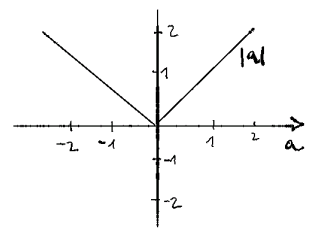
\includegraphics[width=0.4\textwidth]{betrag.png}
    \caption{Betrag verglichen mit 'clipping'. Sinus Schwingung als Input.}
    \label{fig:sinBetrag}
\end{figure}


\subsection{Potenzen, Wurzeln, Logarithmen}
\todo[inline]{Erklärender Text evtl}

\subsubsection{Potenzgesetze}

\important{ 

\emph{\textbf{Potenzgesetze}}

$$ a^n \cdot a^m = a^{n+m}$$ 

$$ \frac{a^n}{a^m} = a^{n-m}$$

$$ (a^n)^m = a^{n\cdot m}$$

$$ a^n \cdot b^n = (a \cdot b)^n$$

$$ \frac{a^n} {b^n} = \left(\frac{a} {b} \right)^n. \: b \neq 0.$$
}

\subsubsection{Wissenschaftliche Notation}
\todo[inline]{Erklärungen}
\important{

$$ x = d\cdot 10^e$$

\begin{itemize}
    \item $d$: Mantisse\footnote{ von Lateinisch 'Zugabe' oder 'Gewinn'. Siehe \cite{wiki:mantisse}}
    \item $e$: Exponent
\end{itemize}
}


\subsubsection{Logarithmen}
Konzeptuell verwandt mit der Wurzel, beantwortet er die frage nach dem Exponenten bei gegebener Basis.

$$ 5 ^2 =25 $$

$$\sqrt[2]{25} = 5$$

$$ log_5 (25) = 2$$

\important{
    Wenn wir eine Gleichung der Art:
    $$ b^x = a $$
    Vorfinden wobei $a$ und $b$ konstanten sind und wir $x$ finden wollen und $a>0$ und $b \neq 1$ dann können wir auflösen:
    \begin{equation}
        log_b(a) = x
    \end{equation}

    Außerdem gilt allgemein:
    \begin{equation}
        log_b(b^x) = x
    \end{equation}

}



Der dekadische Logarithmus ($log_{10}$) ist u.a. praktisch, da er quasi die Frage nach den Stellen einer Zahl im dezimal System beantwortet. Ein Negatives Ergebnis gibt hier an, dass es sich um eine zahl $<1$ handelt und sein wert gibt Aufschluss auf die zahl der 'Nullen' vor dem Komma an:

\begin{itemize}
    

\item  $ log_{10}(100) = 2$
\item  $ log_{10}(1000) = 3$
\item  $ log_{10}(1) = 0$
\item  $ log_{10}(0.01) = -2$
\end{itemize}

Diese 'Eigenschaft' kann zB. benutzt werden um Visualisierungen klarer zu machen, in denen werte mit sehr Unterschiedlichen Größenordnungen Verglichen werden sollen. Siehe Abbildung \ref{fig:time_lin} im Vergleich zu \ref{fig:time_log}. Das \emph{Dezibel} fällt mehr oder weniger in diese Kategorie. 

\textbf{Der Logarithmus von 0 ist undefiniert.} Manchmal stößt man (in Computersystemen zb.) auf Ergebnisse die uns zu sagen scheinen, dass  $log(0)=-\infty$. Das ist nicht korrekt/schlampig. Natürlich scheint sich der Funktionsverlauf diesem 'Wert' anzunähern. Korrekterweise lässt sich sagen: $\lim_{x\to 0} log(x)=-\infty$. 


\subsubsection{Rechenregeln mit dem Logarithmus}
\todo[]{todo}

\important{
\begin{equation}
log_a (u \cdot v) = log_a(u) + log_a(v) \label{eq:logprods}
\end{equation}

\begin{equation}
log_a \left(\frac{u}{v}\right) = log_a(u) - log_a(v) \label{eq:logdivs}
\end{equation}

\begin{equation}
log_a (u ^ v) = v \cdot log_a(u) \label{eq:logexps}
\end{equation}

\begin{equation}
log_a \left( \frac{1}{u} \right) = - log_a(u) \label{eq:logminone}
\end{equation}
}


\begin{question}
    Leite Gleichung \ref{eq:logminone} einmal aus Gleichung \ref{eq:logdivs} und einmal aus Gleichung \ref{eq:logexps} ab! 
\end{question}

\begin{answer}
Zu \ref{eq:logdivs}: \\
Man setzt ein, und hat ein kleines Problem da die variablen Namen dafür ungünstig/verwirrend sind. Wir benennen diese also um für Gl. \ref{eq:logdivs}. Außerdem verwerfen wir die $log_a$ Notation da das $a$ hier stets irrelevant ist:
$$ log \left(\frac{x}{y}\right) = log(x) - log(y).$$ 
Wir setzen $x=1$:
$$ log \left(\frac{1}{y}\right) = log(1) - log(y).$$
Wir wissen dass $log(1) = 0$ da $\forall x \in \mathbb{R} \: , \: x^0 = 1$. 
Daher: $$ log \left(\frac{1}{y}\right) = - log(y).$$ \\

Zu \ref{eq:logexps}: \\
Wenn man im Kopf hat dass $x^{-1}=\frac{1}{x}$ ist klar, dass auch hier einsetzten hilft. Ausgehend von Gl. \ref{eq:logexps} bleiben wir bei der $x, \: y$ Notation:
$$log (x ^ y) = y \cdot log(x).$$
Da wir in Gleichung \ref{eq:logminone} dieses vorfinden: $log_a \left( \frac{1}{u} \right)$ und aber wissen dass wir umformen können zu $log_a ( u^{-1}) $ 
Wir setzten $y=-1$ und sind eigentlich schon fertig:
$$log (x ^ {-1}) = -1 \cdot log(x) = $$
$$log \left( \frac{1}{x} \right) = -log(x)$$

\end{answer} 

\subsubsection{Logarithmen 'Konvertieren'}

Gegeben $log_a(x)$ wie kann man $log_b(x)$ errechnen, also zu anderer Basis 'konvertieren'?

Man dividiert durch den $log_a(b)$:

$$ log_b(x) = \frac{log_a(x)}{log_a(b)}$$

\example{\textbf{Beispiel} \\

Gegeben den natürlichen Logarithmus einer Messung $x$ benötigt man den 2er Logarithmus. Der natürliche Logarithmus der Messgröße $x$ ist ca. $1.61$. 
$$log_2(x) = \frac{ln(x)}{ln(2)} $$
Also:
$$log_2(x) = \frac{1.61}{ln(2)} \approx 2.32$$
In diesem Beispiel war $x=5$ und wir können überprüfen dass $log_2(5) \approx 2.32$.
}
\subsubsection {Dezibel \& $dB_{FS}$}
Speziell wichtig in der (Audio-) Signalverarbeitung: $dB$ (Dezibel, ein Zehntel \emph{Bel}). 
\important{
Das $Bel$ \emph{vergleicht} 2 \emph{Leistungsgrößen}, $P_1$ und $P_2$ und erleichtert uns das Leben indem davon der Logarithmus genommen wird:
$$ L_{Bel} = log_{10} \left(\frac{P_1}{P_2}\right)$$
}

Dadurch dass wir nicht immer mit Leistungsgrößen zu tun haben, sondern manchmal zu diesen konvertieren müssen, findet sich oft der Faktor $2$ in der Formel. Konvertierung vom $Bel$ zum $Dezibel$ macht eine Multiplikation mit 10 erforderlich:

$$L = 20 \cdot log_{10}\left(\frac{x}{x_{ref}}\right)$$

Wobei im im digitalen Fall $dB_{FS}$ ('Fullscale') sich $x_{ref}$  auf den Vollausschlag $1$ bezieht und damit vereinfacht werden kann zu: 
$$L = 20 \cdot log_{10}(x)$$

\todo[]{Exkurs: Leistung eines digitalsignals via URI}
\todo[]{Andere Referenzwerte.}

\faust{Lineare Lautstärken Steuerung verglichen mit klassisch Logarithmischer.}{https://faustide.grame.fr/?autorun=1&voices=0&name=example&inline=aW1wb3J0KCJzdGRmYXVzdC5saWIiKTsKYW1wID0gaHNsaWRlcigiTGluZWFyIEFtcGxpdHVkZSIsIDAuLCAwLCAxLCAwLjAwMSk6c2kuc21vbzsKCmFtcExvZyA9IGhzbGlkZXIoIkxvZyBBbXBsaXR1ZGUiLCAtNzAuLCAtNzAsIDAsIDAuMDEpOnNpLnNtb286YmEuZGIybGluZWFyOwoKcHJvY2VzcyA9IG5vLnBpbmtfbm9pc2UgKiBhbXAgKyBuby5waW5rX25vaXNlICogYW1wTG9nPDpfLF87}

\todo[]{Wurzeln}



\begin{figure}[h!]
    \centering
    %% Creator: Matplotlib, PGF backend
%%
%% To include the figure in your LaTeX document, write
%%   \input{<filename>.pgf}
%%
%% Make sure the required packages are loaded in your preamble
%%   \usepackage{pgf}
%%
%% Also ensure that all the required font packages are loaded; for instance,
%% the lmodern package is sometimes necessary when using math font.
%%   \usepackage{lmodern}
%%
%% Figures using additional raster images can only be included by \input if
%% they are in the same directory as the main LaTeX file. For loading figures
%% from other directories you can use the `import` package
%%   \usepackage{import}
%%
%% and then include the figures with
%%   \import{<path to file>}{<filename>.pgf}
%%
%% Matplotlib used the following preamble
%%   \def\mathdefault#1{#1}
%%   \everymath=\expandafter{\the\everymath\displaystyle}
%%   \usepackage{amsmath}
%%   \makeatletter\@ifpackageloaded{underscore}{}{\usepackage[strings]{underscore}}\makeatother
%%
\begingroup%
\makeatletter%
\begin{pgfpicture}%
\pgfpathrectangle{\pgfpointorigin}{\pgfqpoint{5.504137in}{4.320382in}}%
\pgfusepath{use as bounding box, clip}%
\begin{pgfscope}%
\pgfsetbuttcap%
\pgfsetmiterjoin%
\definecolor{currentfill}{rgb}{1.000000,1.000000,1.000000}%
\pgfsetfillcolor{currentfill}%
\pgfsetlinewidth{0.000000pt}%
\definecolor{currentstroke}{rgb}{1.000000,1.000000,1.000000}%
\pgfsetstrokecolor{currentstroke}%
\pgfsetdash{}{0pt}%
\pgfpathmoveto{\pgfqpoint{0.000000in}{0.000000in}}%
\pgfpathlineto{\pgfqpoint{5.504137in}{0.000000in}}%
\pgfpathlineto{\pgfqpoint{5.504137in}{4.320382in}}%
\pgfpathlineto{\pgfqpoint{0.000000in}{4.320382in}}%
\pgfpathlineto{\pgfqpoint{0.000000in}{0.000000in}}%
\pgfpathclose%
\pgfusepath{fill}%
\end{pgfscope}%
\begin{pgfscope}%
\pgfsetbuttcap%
\pgfsetmiterjoin%
\definecolor{currentfill}{rgb}{1.000000,1.000000,1.000000}%
\pgfsetfillcolor{currentfill}%
\pgfsetlinewidth{0.000000pt}%
\definecolor{currentstroke}{rgb}{0.000000,0.000000,0.000000}%
\pgfsetstrokecolor{currentstroke}%
\pgfsetstrokeopacity{0.000000}%
\pgfsetdash{}{0pt}%
\pgfpathmoveto{\pgfqpoint{0.444137in}{0.524382in}}%
\pgfpathlineto{\pgfqpoint{5.404137in}{0.524382in}}%
\pgfpathlineto{\pgfqpoint{5.404137in}{4.220382in}}%
\pgfpathlineto{\pgfqpoint{0.444137in}{4.220382in}}%
\pgfpathlineto{\pgfqpoint{0.444137in}{0.524382in}}%
\pgfpathclose%
\pgfusepath{fill}%
\end{pgfscope}%
\begin{pgfscope}%
\pgfpathrectangle{\pgfqpoint{0.444137in}{0.524382in}}{\pgfqpoint{4.960000in}{3.696000in}}%
\pgfusepath{clip}%
\pgfsetrectcap%
\pgfsetroundjoin%
\pgfsetlinewidth{0.803000pt}%
\definecolor{currentstroke}{rgb}{0.690196,0.690196,0.690196}%
\pgfsetstrokecolor{currentstroke}%
\pgfsetdash{}{0pt}%
\pgfpathmoveto{\pgfqpoint{0.667787in}{0.524382in}}%
\pgfpathlineto{\pgfqpoint{0.667787in}{4.220382in}}%
\pgfusepath{stroke}%
\end{pgfscope}%
\begin{pgfscope}%
\pgfsetbuttcap%
\pgfsetroundjoin%
\definecolor{currentfill}{rgb}{0.000000,0.000000,0.000000}%
\pgfsetfillcolor{currentfill}%
\pgfsetlinewidth{0.803000pt}%
\definecolor{currentstroke}{rgb}{0.000000,0.000000,0.000000}%
\pgfsetstrokecolor{currentstroke}%
\pgfsetdash{}{0pt}%
\pgfsys@defobject{currentmarker}{\pgfqpoint{0.000000in}{-0.048611in}}{\pgfqpoint{0.000000in}{0.000000in}}{%
\pgfpathmoveto{\pgfqpoint{0.000000in}{0.000000in}}%
\pgfpathlineto{\pgfqpoint{0.000000in}{-0.048611in}}%
\pgfusepath{stroke,fill}%
}%
\begin{pgfscope}%
\pgfsys@transformshift{0.667787in}{0.524382in}%
\pgfsys@useobject{currentmarker}{}%
\end{pgfscope}%
\end{pgfscope}%
\begin{pgfscope}%
\definecolor{textcolor}{rgb}{0.000000,0.000000,0.000000}%
\pgfsetstrokecolor{textcolor}%
\pgfsetfillcolor{textcolor}%
\pgftext[x=0.667787in,y=0.427160in,,top]{\color{textcolor}{\rmfamily\fontsize{10.000000}{12.000000}\selectfont\catcode`\^=\active\def^{\ifmmode\sp\else\^{}\fi}\catcode`\%=\active\def%{\%}0.0}}%
\end{pgfscope}%
\begin{pgfscope}%
\pgfpathrectangle{\pgfqpoint{0.444137in}{0.524382in}}{\pgfqpoint{4.960000in}{3.696000in}}%
\pgfusepath{clip}%
\pgfsetrectcap%
\pgfsetroundjoin%
\pgfsetlinewidth{0.803000pt}%
\definecolor{currentstroke}{rgb}{0.690196,0.690196,0.690196}%
\pgfsetstrokecolor{currentstroke}%
\pgfsetdash{}{0pt}%
\pgfpathmoveto{\pgfqpoint{1.569966in}{0.524382in}}%
\pgfpathlineto{\pgfqpoint{1.569966in}{4.220382in}}%
\pgfusepath{stroke}%
\end{pgfscope}%
\begin{pgfscope}%
\pgfsetbuttcap%
\pgfsetroundjoin%
\definecolor{currentfill}{rgb}{0.000000,0.000000,0.000000}%
\pgfsetfillcolor{currentfill}%
\pgfsetlinewidth{0.803000pt}%
\definecolor{currentstroke}{rgb}{0.000000,0.000000,0.000000}%
\pgfsetstrokecolor{currentstroke}%
\pgfsetdash{}{0pt}%
\pgfsys@defobject{currentmarker}{\pgfqpoint{0.000000in}{-0.048611in}}{\pgfqpoint{0.000000in}{0.000000in}}{%
\pgfpathmoveto{\pgfqpoint{0.000000in}{0.000000in}}%
\pgfpathlineto{\pgfqpoint{0.000000in}{-0.048611in}}%
\pgfusepath{stroke,fill}%
}%
\begin{pgfscope}%
\pgfsys@transformshift{1.569966in}{0.524382in}%
\pgfsys@useobject{currentmarker}{}%
\end{pgfscope}%
\end{pgfscope}%
\begin{pgfscope}%
\definecolor{textcolor}{rgb}{0.000000,0.000000,0.000000}%
\pgfsetstrokecolor{textcolor}%
\pgfsetfillcolor{textcolor}%
\pgftext[x=1.569966in,y=0.427160in,,top]{\color{textcolor}{\rmfamily\fontsize{10.000000}{12.000000}\selectfont\catcode`\^=\active\def^{\ifmmode\sp\else\^{}\fi}\catcode`\%=\active\def%{\%}0.5}}%
\end{pgfscope}%
\begin{pgfscope}%
\pgfpathrectangle{\pgfqpoint{0.444137in}{0.524382in}}{\pgfqpoint{4.960000in}{3.696000in}}%
\pgfusepath{clip}%
\pgfsetrectcap%
\pgfsetroundjoin%
\pgfsetlinewidth{0.803000pt}%
\definecolor{currentstroke}{rgb}{0.690196,0.690196,0.690196}%
\pgfsetstrokecolor{currentstroke}%
\pgfsetdash{}{0pt}%
\pgfpathmoveto{\pgfqpoint{2.472145in}{0.524382in}}%
\pgfpathlineto{\pgfqpoint{2.472145in}{4.220382in}}%
\pgfusepath{stroke}%
\end{pgfscope}%
\begin{pgfscope}%
\pgfsetbuttcap%
\pgfsetroundjoin%
\definecolor{currentfill}{rgb}{0.000000,0.000000,0.000000}%
\pgfsetfillcolor{currentfill}%
\pgfsetlinewidth{0.803000pt}%
\definecolor{currentstroke}{rgb}{0.000000,0.000000,0.000000}%
\pgfsetstrokecolor{currentstroke}%
\pgfsetdash{}{0pt}%
\pgfsys@defobject{currentmarker}{\pgfqpoint{0.000000in}{-0.048611in}}{\pgfqpoint{0.000000in}{0.000000in}}{%
\pgfpathmoveto{\pgfqpoint{0.000000in}{0.000000in}}%
\pgfpathlineto{\pgfqpoint{0.000000in}{-0.048611in}}%
\pgfusepath{stroke,fill}%
}%
\begin{pgfscope}%
\pgfsys@transformshift{2.472145in}{0.524382in}%
\pgfsys@useobject{currentmarker}{}%
\end{pgfscope}%
\end{pgfscope}%
\begin{pgfscope}%
\definecolor{textcolor}{rgb}{0.000000,0.000000,0.000000}%
\pgfsetstrokecolor{textcolor}%
\pgfsetfillcolor{textcolor}%
\pgftext[x=2.472145in,y=0.427160in,,top]{\color{textcolor}{\rmfamily\fontsize{10.000000}{12.000000}\selectfont\catcode`\^=\active\def^{\ifmmode\sp\else\^{}\fi}\catcode`\%=\active\def%{\%}1.0}}%
\end{pgfscope}%
\begin{pgfscope}%
\pgfpathrectangle{\pgfqpoint{0.444137in}{0.524382in}}{\pgfqpoint{4.960000in}{3.696000in}}%
\pgfusepath{clip}%
\pgfsetrectcap%
\pgfsetroundjoin%
\pgfsetlinewidth{0.803000pt}%
\definecolor{currentstroke}{rgb}{0.690196,0.690196,0.690196}%
\pgfsetstrokecolor{currentstroke}%
\pgfsetdash{}{0pt}%
\pgfpathmoveto{\pgfqpoint{3.374324in}{0.524382in}}%
\pgfpathlineto{\pgfqpoint{3.374324in}{4.220382in}}%
\pgfusepath{stroke}%
\end{pgfscope}%
\begin{pgfscope}%
\pgfsetbuttcap%
\pgfsetroundjoin%
\definecolor{currentfill}{rgb}{0.000000,0.000000,0.000000}%
\pgfsetfillcolor{currentfill}%
\pgfsetlinewidth{0.803000pt}%
\definecolor{currentstroke}{rgb}{0.000000,0.000000,0.000000}%
\pgfsetstrokecolor{currentstroke}%
\pgfsetdash{}{0pt}%
\pgfsys@defobject{currentmarker}{\pgfqpoint{0.000000in}{-0.048611in}}{\pgfqpoint{0.000000in}{0.000000in}}{%
\pgfpathmoveto{\pgfqpoint{0.000000in}{0.000000in}}%
\pgfpathlineto{\pgfqpoint{0.000000in}{-0.048611in}}%
\pgfusepath{stroke,fill}%
}%
\begin{pgfscope}%
\pgfsys@transformshift{3.374324in}{0.524382in}%
\pgfsys@useobject{currentmarker}{}%
\end{pgfscope}%
\end{pgfscope}%
\begin{pgfscope}%
\definecolor{textcolor}{rgb}{0.000000,0.000000,0.000000}%
\pgfsetstrokecolor{textcolor}%
\pgfsetfillcolor{textcolor}%
\pgftext[x=3.374324in,y=0.427160in,,top]{\color{textcolor}{\rmfamily\fontsize{10.000000}{12.000000}\selectfont\catcode`\^=\active\def^{\ifmmode\sp\else\^{}\fi}\catcode`\%=\active\def%{\%}1.5}}%
\end{pgfscope}%
\begin{pgfscope}%
\pgfpathrectangle{\pgfqpoint{0.444137in}{0.524382in}}{\pgfqpoint{4.960000in}{3.696000in}}%
\pgfusepath{clip}%
\pgfsetrectcap%
\pgfsetroundjoin%
\pgfsetlinewidth{0.803000pt}%
\definecolor{currentstroke}{rgb}{0.690196,0.690196,0.690196}%
\pgfsetstrokecolor{currentstroke}%
\pgfsetdash{}{0pt}%
\pgfpathmoveto{\pgfqpoint{4.276503in}{0.524382in}}%
\pgfpathlineto{\pgfqpoint{4.276503in}{4.220382in}}%
\pgfusepath{stroke}%
\end{pgfscope}%
\begin{pgfscope}%
\pgfsetbuttcap%
\pgfsetroundjoin%
\definecolor{currentfill}{rgb}{0.000000,0.000000,0.000000}%
\pgfsetfillcolor{currentfill}%
\pgfsetlinewidth{0.803000pt}%
\definecolor{currentstroke}{rgb}{0.000000,0.000000,0.000000}%
\pgfsetstrokecolor{currentstroke}%
\pgfsetdash{}{0pt}%
\pgfsys@defobject{currentmarker}{\pgfqpoint{0.000000in}{-0.048611in}}{\pgfqpoint{0.000000in}{0.000000in}}{%
\pgfpathmoveto{\pgfqpoint{0.000000in}{0.000000in}}%
\pgfpathlineto{\pgfqpoint{0.000000in}{-0.048611in}}%
\pgfusepath{stroke,fill}%
}%
\begin{pgfscope}%
\pgfsys@transformshift{4.276503in}{0.524382in}%
\pgfsys@useobject{currentmarker}{}%
\end{pgfscope}%
\end{pgfscope}%
\begin{pgfscope}%
\definecolor{textcolor}{rgb}{0.000000,0.000000,0.000000}%
\pgfsetstrokecolor{textcolor}%
\pgfsetfillcolor{textcolor}%
\pgftext[x=4.276503in,y=0.427160in,,top]{\color{textcolor}{\rmfamily\fontsize{10.000000}{12.000000}\selectfont\catcode`\^=\active\def^{\ifmmode\sp\else\^{}\fi}\catcode`\%=\active\def%{\%}2.0}}%
\end{pgfscope}%
\begin{pgfscope}%
\pgfpathrectangle{\pgfqpoint{0.444137in}{0.524382in}}{\pgfqpoint{4.960000in}{3.696000in}}%
\pgfusepath{clip}%
\pgfsetrectcap%
\pgfsetroundjoin%
\pgfsetlinewidth{0.803000pt}%
\definecolor{currentstroke}{rgb}{0.690196,0.690196,0.690196}%
\pgfsetstrokecolor{currentstroke}%
\pgfsetdash{}{0pt}%
\pgfpathmoveto{\pgfqpoint{5.178682in}{0.524382in}}%
\pgfpathlineto{\pgfqpoint{5.178682in}{4.220382in}}%
\pgfusepath{stroke}%
\end{pgfscope}%
\begin{pgfscope}%
\pgfsetbuttcap%
\pgfsetroundjoin%
\definecolor{currentfill}{rgb}{0.000000,0.000000,0.000000}%
\pgfsetfillcolor{currentfill}%
\pgfsetlinewidth{0.803000pt}%
\definecolor{currentstroke}{rgb}{0.000000,0.000000,0.000000}%
\pgfsetstrokecolor{currentstroke}%
\pgfsetdash{}{0pt}%
\pgfsys@defobject{currentmarker}{\pgfqpoint{0.000000in}{-0.048611in}}{\pgfqpoint{0.000000in}{0.000000in}}{%
\pgfpathmoveto{\pgfqpoint{0.000000in}{0.000000in}}%
\pgfpathlineto{\pgfqpoint{0.000000in}{-0.048611in}}%
\pgfusepath{stroke,fill}%
}%
\begin{pgfscope}%
\pgfsys@transformshift{5.178682in}{0.524382in}%
\pgfsys@useobject{currentmarker}{}%
\end{pgfscope}%
\end{pgfscope}%
\begin{pgfscope}%
\definecolor{textcolor}{rgb}{0.000000,0.000000,0.000000}%
\pgfsetstrokecolor{textcolor}%
\pgfsetfillcolor{textcolor}%
\pgftext[x=5.178682in,y=0.427160in,,top]{\color{textcolor}{\rmfamily\fontsize{10.000000}{12.000000}\selectfont\catcode`\^=\active\def^{\ifmmode\sp\else\^{}\fi}\catcode`\%=\active\def%{\%}2.5}}%
\end{pgfscope}%
\begin{pgfscope}%
\definecolor{textcolor}{rgb}{0.000000,0.000000,0.000000}%
\pgfsetstrokecolor{textcolor}%
\pgfsetfillcolor{textcolor}%
\pgftext[x=2.924137in,y=0.248148in,,top]{\color{textcolor}{\rmfamily\fontsize{12.000000}{14.400000}\selectfont\catcode`\^=\active\def^{\ifmmode\sp\else\^{}\fi}\catcode`\%=\active\def%{\%}$x$}}%
\end{pgfscope}%
\begin{pgfscope}%
\pgfpathrectangle{\pgfqpoint{0.444137in}{0.524382in}}{\pgfqpoint{4.960000in}{3.696000in}}%
\pgfusepath{clip}%
\pgfsetrectcap%
\pgfsetroundjoin%
\pgfsetlinewidth{0.803000pt}%
\definecolor{currentstroke}{rgb}{0.690196,0.690196,0.690196}%
\pgfsetstrokecolor{currentstroke}%
\pgfsetdash{}{0pt}%
\pgfpathmoveto{\pgfqpoint{0.444137in}{0.692382in}}%
\pgfpathlineto{\pgfqpoint{5.404137in}{0.692382in}}%
\pgfusepath{stroke}%
\end{pgfscope}%
\begin{pgfscope}%
\pgfsetbuttcap%
\pgfsetroundjoin%
\definecolor{currentfill}{rgb}{0.000000,0.000000,0.000000}%
\pgfsetfillcolor{currentfill}%
\pgfsetlinewidth{0.803000pt}%
\definecolor{currentstroke}{rgb}{0.000000,0.000000,0.000000}%
\pgfsetstrokecolor{currentstroke}%
\pgfsetdash{}{0pt}%
\pgfsys@defobject{currentmarker}{\pgfqpoint{-0.048611in}{0.000000in}}{\pgfqpoint{-0.000000in}{0.000000in}}{%
\pgfpathmoveto{\pgfqpoint{-0.000000in}{0.000000in}}%
\pgfpathlineto{\pgfqpoint{-0.048611in}{0.000000in}}%
\pgfusepath{stroke,fill}%
}%
\begin{pgfscope}%
\pgfsys@transformshift{0.444137in}{0.692382in}%
\pgfsys@useobject{currentmarker}{}%
\end{pgfscope}%
\end{pgfscope}%
\begin{pgfscope}%
\definecolor{textcolor}{rgb}{0.000000,0.000000,0.000000}%
\pgfsetstrokecolor{textcolor}%
\pgfsetfillcolor{textcolor}%
\pgftext[x=0.100000in, y=0.644157in, left, base]{\color{textcolor}{\rmfamily\fontsize{10.000000}{12.000000}\selectfont\catcode`\^=\active\def^{\ifmmode\sp\else\^{}\fi}\catcode`\%=\active\def%{\%}\ensuremath{-}60}}%
\end{pgfscope}%
\begin{pgfscope}%
\pgfpathrectangle{\pgfqpoint{0.444137in}{0.524382in}}{\pgfqpoint{4.960000in}{3.696000in}}%
\pgfusepath{clip}%
\pgfsetrectcap%
\pgfsetroundjoin%
\pgfsetlinewidth{0.803000pt}%
\definecolor{currentstroke}{rgb}{0.690196,0.690196,0.690196}%
\pgfsetstrokecolor{currentstroke}%
\pgfsetdash{}{0pt}%
\pgfpathmoveto{\pgfqpoint{0.444137in}{1.186799in}}%
\pgfpathlineto{\pgfqpoint{5.404137in}{1.186799in}}%
\pgfusepath{stroke}%
\end{pgfscope}%
\begin{pgfscope}%
\pgfsetbuttcap%
\pgfsetroundjoin%
\definecolor{currentfill}{rgb}{0.000000,0.000000,0.000000}%
\pgfsetfillcolor{currentfill}%
\pgfsetlinewidth{0.803000pt}%
\definecolor{currentstroke}{rgb}{0.000000,0.000000,0.000000}%
\pgfsetstrokecolor{currentstroke}%
\pgfsetdash{}{0pt}%
\pgfsys@defobject{currentmarker}{\pgfqpoint{-0.048611in}{0.000000in}}{\pgfqpoint{-0.000000in}{0.000000in}}{%
\pgfpathmoveto{\pgfqpoint{-0.000000in}{0.000000in}}%
\pgfpathlineto{\pgfqpoint{-0.048611in}{0.000000in}}%
\pgfusepath{stroke,fill}%
}%
\begin{pgfscope}%
\pgfsys@transformshift{0.444137in}{1.186799in}%
\pgfsys@useobject{currentmarker}{}%
\end{pgfscope}%
\end{pgfscope}%
\begin{pgfscope}%
\definecolor{textcolor}{rgb}{0.000000,0.000000,0.000000}%
\pgfsetstrokecolor{textcolor}%
\pgfsetfillcolor{textcolor}%
\pgftext[x=0.100000in, y=1.138574in, left, base]{\color{textcolor}{\rmfamily\fontsize{10.000000}{12.000000}\selectfont\catcode`\^=\active\def^{\ifmmode\sp\else\^{}\fi}\catcode`\%=\active\def%{\%}\ensuremath{-}50}}%
\end{pgfscope}%
\begin{pgfscope}%
\pgfpathrectangle{\pgfqpoint{0.444137in}{0.524382in}}{\pgfqpoint{4.960000in}{3.696000in}}%
\pgfusepath{clip}%
\pgfsetrectcap%
\pgfsetroundjoin%
\pgfsetlinewidth{0.803000pt}%
\definecolor{currentstroke}{rgb}{0.690196,0.690196,0.690196}%
\pgfsetstrokecolor{currentstroke}%
\pgfsetdash{}{0pt}%
\pgfpathmoveto{\pgfqpoint{0.444137in}{1.681216in}}%
\pgfpathlineto{\pgfqpoint{5.404137in}{1.681216in}}%
\pgfusepath{stroke}%
\end{pgfscope}%
\begin{pgfscope}%
\pgfsetbuttcap%
\pgfsetroundjoin%
\definecolor{currentfill}{rgb}{0.000000,0.000000,0.000000}%
\pgfsetfillcolor{currentfill}%
\pgfsetlinewidth{0.803000pt}%
\definecolor{currentstroke}{rgb}{0.000000,0.000000,0.000000}%
\pgfsetstrokecolor{currentstroke}%
\pgfsetdash{}{0pt}%
\pgfsys@defobject{currentmarker}{\pgfqpoint{-0.048611in}{0.000000in}}{\pgfqpoint{-0.000000in}{0.000000in}}{%
\pgfpathmoveto{\pgfqpoint{-0.000000in}{0.000000in}}%
\pgfpathlineto{\pgfqpoint{-0.048611in}{0.000000in}}%
\pgfusepath{stroke,fill}%
}%
\begin{pgfscope}%
\pgfsys@transformshift{0.444137in}{1.681216in}%
\pgfsys@useobject{currentmarker}{}%
\end{pgfscope}%
\end{pgfscope}%
\begin{pgfscope}%
\definecolor{textcolor}{rgb}{0.000000,0.000000,0.000000}%
\pgfsetstrokecolor{textcolor}%
\pgfsetfillcolor{textcolor}%
\pgftext[x=0.100000in, y=1.632991in, left, base]{\color{textcolor}{\rmfamily\fontsize{10.000000}{12.000000}\selectfont\catcode`\^=\active\def^{\ifmmode\sp\else\^{}\fi}\catcode`\%=\active\def%{\%}\ensuremath{-}40}}%
\end{pgfscope}%
\begin{pgfscope}%
\pgfpathrectangle{\pgfqpoint{0.444137in}{0.524382in}}{\pgfqpoint{4.960000in}{3.696000in}}%
\pgfusepath{clip}%
\pgfsetrectcap%
\pgfsetroundjoin%
\pgfsetlinewidth{0.803000pt}%
\definecolor{currentstroke}{rgb}{0.690196,0.690196,0.690196}%
\pgfsetstrokecolor{currentstroke}%
\pgfsetdash{}{0pt}%
\pgfpathmoveto{\pgfqpoint{0.444137in}{2.175634in}}%
\pgfpathlineto{\pgfqpoint{5.404137in}{2.175634in}}%
\pgfusepath{stroke}%
\end{pgfscope}%
\begin{pgfscope}%
\pgfsetbuttcap%
\pgfsetroundjoin%
\definecolor{currentfill}{rgb}{0.000000,0.000000,0.000000}%
\pgfsetfillcolor{currentfill}%
\pgfsetlinewidth{0.803000pt}%
\definecolor{currentstroke}{rgb}{0.000000,0.000000,0.000000}%
\pgfsetstrokecolor{currentstroke}%
\pgfsetdash{}{0pt}%
\pgfsys@defobject{currentmarker}{\pgfqpoint{-0.048611in}{0.000000in}}{\pgfqpoint{-0.000000in}{0.000000in}}{%
\pgfpathmoveto{\pgfqpoint{-0.000000in}{0.000000in}}%
\pgfpathlineto{\pgfqpoint{-0.048611in}{0.000000in}}%
\pgfusepath{stroke,fill}%
}%
\begin{pgfscope}%
\pgfsys@transformshift{0.444137in}{2.175634in}%
\pgfsys@useobject{currentmarker}{}%
\end{pgfscope}%
\end{pgfscope}%
\begin{pgfscope}%
\definecolor{textcolor}{rgb}{0.000000,0.000000,0.000000}%
\pgfsetstrokecolor{textcolor}%
\pgfsetfillcolor{textcolor}%
\pgftext[x=0.100000in, y=2.127408in, left, base]{\color{textcolor}{\rmfamily\fontsize{10.000000}{12.000000}\selectfont\catcode`\^=\active\def^{\ifmmode\sp\else\^{}\fi}\catcode`\%=\active\def%{\%}\ensuremath{-}30}}%
\end{pgfscope}%
\begin{pgfscope}%
\pgfpathrectangle{\pgfqpoint{0.444137in}{0.524382in}}{\pgfqpoint{4.960000in}{3.696000in}}%
\pgfusepath{clip}%
\pgfsetrectcap%
\pgfsetroundjoin%
\pgfsetlinewidth{0.803000pt}%
\definecolor{currentstroke}{rgb}{0.690196,0.690196,0.690196}%
\pgfsetstrokecolor{currentstroke}%
\pgfsetdash{}{0pt}%
\pgfpathmoveto{\pgfqpoint{0.444137in}{2.670051in}}%
\pgfpathlineto{\pgfqpoint{5.404137in}{2.670051in}}%
\pgfusepath{stroke}%
\end{pgfscope}%
\begin{pgfscope}%
\pgfsetbuttcap%
\pgfsetroundjoin%
\definecolor{currentfill}{rgb}{0.000000,0.000000,0.000000}%
\pgfsetfillcolor{currentfill}%
\pgfsetlinewidth{0.803000pt}%
\definecolor{currentstroke}{rgb}{0.000000,0.000000,0.000000}%
\pgfsetstrokecolor{currentstroke}%
\pgfsetdash{}{0pt}%
\pgfsys@defobject{currentmarker}{\pgfqpoint{-0.048611in}{0.000000in}}{\pgfqpoint{-0.000000in}{0.000000in}}{%
\pgfpathmoveto{\pgfqpoint{-0.000000in}{0.000000in}}%
\pgfpathlineto{\pgfqpoint{-0.048611in}{0.000000in}}%
\pgfusepath{stroke,fill}%
}%
\begin{pgfscope}%
\pgfsys@transformshift{0.444137in}{2.670051in}%
\pgfsys@useobject{currentmarker}{}%
\end{pgfscope}%
\end{pgfscope}%
\begin{pgfscope}%
\definecolor{textcolor}{rgb}{0.000000,0.000000,0.000000}%
\pgfsetstrokecolor{textcolor}%
\pgfsetfillcolor{textcolor}%
\pgftext[x=0.100000in, y=2.621825in, left, base]{\color{textcolor}{\rmfamily\fontsize{10.000000}{12.000000}\selectfont\catcode`\^=\active\def^{\ifmmode\sp\else\^{}\fi}\catcode`\%=\active\def%{\%}\ensuremath{-}20}}%
\end{pgfscope}%
\begin{pgfscope}%
\pgfpathrectangle{\pgfqpoint{0.444137in}{0.524382in}}{\pgfqpoint{4.960000in}{3.696000in}}%
\pgfusepath{clip}%
\pgfsetrectcap%
\pgfsetroundjoin%
\pgfsetlinewidth{0.803000pt}%
\definecolor{currentstroke}{rgb}{0.690196,0.690196,0.690196}%
\pgfsetstrokecolor{currentstroke}%
\pgfsetdash{}{0pt}%
\pgfpathmoveto{\pgfqpoint{0.444137in}{3.164468in}}%
\pgfpathlineto{\pgfqpoint{5.404137in}{3.164468in}}%
\pgfusepath{stroke}%
\end{pgfscope}%
\begin{pgfscope}%
\pgfsetbuttcap%
\pgfsetroundjoin%
\definecolor{currentfill}{rgb}{0.000000,0.000000,0.000000}%
\pgfsetfillcolor{currentfill}%
\pgfsetlinewidth{0.803000pt}%
\definecolor{currentstroke}{rgb}{0.000000,0.000000,0.000000}%
\pgfsetstrokecolor{currentstroke}%
\pgfsetdash{}{0pt}%
\pgfsys@defobject{currentmarker}{\pgfqpoint{-0.048611in}{0.000000in}}{\pgfqpoint{-0.000000in}{0.000000in}}{%
\pgfpathmoveto{\pgfqpoint{-0.000000in}{0.000000in}}%
\pgfpathlineto{\pgfqpoint{-0.048611in}{0.000000in}}%
\pgfusepath{stroke,fill}%
}%
\begin{pgfscope}%
\pgfsys@transformshift{0.444137in}{3.164468in}%
\pgfsys@useobject{currentmarker}{}%
\end{pgfscope}%
\end{pgfscope}%
\begin{pgfscope}%
\definecolor{textcolor}{rgb}{0.000000,0.000000,0.000000}%
\pgfsetstrokecolor{textcolor}%
\pgfsetfillcolor{textcolor}%
\pgftext[x=0.100000in, y=3.116243in, left, base]{\color{textcolor}{\rmfamily\fontsize{10.000000}{12.000000}\selectfont\catcode`\^=\active\def^{\ifmmode\sp\else\^{}\fi}\catcode`\%=\active\def%{\%}\ensuremath{-}10}}%
\end{pgfscope}%
\begin{pgfscope}%
\pgfpathrectangle{\pgfqpoint{0.444137in}{0.524382in}}{\pgfqpoint{4.960000in}{3.696000in}}%
\pgfusepath{clip}%
\pgfsetrectcap%
\pgfsetroundjoin%
\pgfsetlinewidth{0.803000pt}%
\definecolor{currentstroke}{rgb}{0.690196,0.690196,0.690196}%
\pgfsetstrokecolor{currentstroke}%
\pgfsetdash{}{0pt}%
\pgfpathmoveto{\pgfqpoint{0.444137in}{3.658885in}}%
\pgfpathlineto{\pgfqpoint{5.404137in}{3.658885in}}%
\pgfusepath{stroke}%
\end{pgfscope}%
\begin{pgfscope}%
\pgfsetbuttcap%
\pgfsetroundjoin%
\definecolor{currentfill}{rgb}{0.000000,0.000000,0.000000}%
\pgfsetfillcolor{currentfill}%
\pgfsetlinewidth{0.803000pt}%
\definecolor{currentstroke}{rgb}{0.000000,0.000000,0.000000}%
\pgfsetstrokecolor{currentstroke}%
\pgfsetdash{}{0pt}%
\pgfsys@defobject{currentmarker}{\pgfqpoint{-0.048611in}{0.000000in}}{\pgfqpoint{-0.000000in}{0.000000in}}{%
\pgfpathmoveto{\pgfqpoint{-0.000000in}{0.000000in}}%
\pgfpathlineto{\pgfqpoint{-0.048611in}{0.000000in}}%
\pgfusepath{stroke,fill}%
}%
\begin{pgfscope}%
\pgfsys@transformshift{0.444137in}{3.658885in}%
\pgfsys@useobject{currentmarker}{}%
\end{pgfscope}%
\end{pgfscope}%
\begin{pgfscope}%
\definecolor{textcolor}{rgb}{0.000000,0.000000,0.000000}%
\pgfsetstrokecolor{textcolor}%
\pgfsetfillcolor{textcolor}%
\pgftext[x=0.277470in, y=3.610660in, left, base]{\color{textcolor}{\rmfamily\fontsize{10.000000}{12.000000}\selectfont\catcode`\^=\active\def^{\ifmmode\sp\else\^{}\fi}\catcode`\%=\active\def%{\%}0}}%
\end{pgfscope}%
\begin{pgfscope}%
\pgfpathrectangle{\pgfqpoint{0.444137in}{0.524382in}}{\pgfqpoint{4.960000in}{3.696000in}}%
\pgfusepath{clip}%
\pgfsetrectcap%
\pgfsetroundjoin%
\pgfsetlinewidth{0.803000pt}%
\definecolor{currentstroke}{rgb}{0.690196,0.690196,0.690196}%
\pgfsetstrokecolor{currentstroke}%
\pgfsetdash{}{0pt}%
\pgfpathmoveto{\pgfqpoint{0.444137in}{4.153302in}}%
\pgfpathlineto{\pgfqpoint{5.404137in}{4.153302in}}%
\pgfusepath{stroke}%
\end{pgfscope}%
\begin{pgfscope}%
\pgfsetbuttcap%
\pgfsetroundjoin%
\definecolor{currentfill}{rgb}{0.000000,0.000000,0.000000}%
\pgfsetfillcolor{currentfill}%
\pgfsetlinewidth{0.803000pt}%
\definecolor{currentstroke}{rgb}{0.000000,0.000000,0.000000}%
\pgfsetstrokecolor{currentstroke}%
\pgfsetdash{}{0pt}%
\pgfsys@defobject{currentmarker}{\pgfqpoint{-0.048611in}{0.000000in}}{\pgfqpoint{-0.000000in}{0.000000in}}{%
\pgfpathmoveto{\pgfqpoint{-0.000000in}{0.000000in}}%
\pgfpathlineto{\pgfqpoint{-0.048611in}{0.000000in}}%
\pgfusepath{stroke,fill}%
}%
\begin{pgfscope}%
\pgfsys@transformshift{0.444137in}{4.153302in}%
\pgfsys@useobject{currentmarker}{}%
\end{pgfscope}%
\end{pgfscope}%
\begin{pgfscope}%
\definecolor{textcolor}{rgb}{0.000000,0.000000,0.000000}%
\pgfsetstrokecolor{textcolor}%
\pgfsetfillcolor{textcolor}%
\pgftext[x=0.208025in, y=4.105077in, left, base]{\color{textcolor}{\rmfamily\fontsize{10.000000}{12.000000}\selectfont\catcode`\^=\active\def^{\ifmmode\sp\else\^{}\fi}\catcode`\%=\active\def%{\%}10}}%
\end{pgfscope}%
\begin{pgfscope}%
\pgfpathrectangle{\pgfqpoint{0.444137in}{0.524382in}}{\pgfqpoint{4.960000in}{3.696000in}}%
\pgfusepath{clip}%
\pgfsetrectcap%
\pgfsetroundjoin%
\pgfsetlinewidth{1.505625pt}%
\definecolor{currentstroke}{rgb}{0.000000,0.000000,0.000000}%
\pgfsetstrokecolor{currentstroke}%
\pgfsetdash{}{0pt}%
\pgfpathmoveto{\pgfqpoint{0.669591in}{0.692382in}}%
\pgfpathlineto{\pgfqpoint{0.674105in}{1.230559in}}%
\pgfpathlineto{\pgfqpoint{0.678618in}{1.462060in}}%
\pgfpathlineto{\pgfqpoint{0.683132in}{1.611651in}}%
\pgfpathlineto{\pgfqpoint{0.692159in}{1.810334in}}%
\pgfpathlineto{\pgfqpoint{0.701186in}{1.945649in}}%
\pgfpathlineto{\pgfqpoint{0.710214in}{2.048388in}}%
\pgfpathlineto{\pgfqpoint{0.719241in}{2.131231in}}%
\pgfpathlineto{\pgfqpoint{0.732782in}{2.231558in}}%
\pgfpathlineto{\pgfqpoint{0.746322in}{2.312828in}}%
\pgfpathlineto{\pgfqpoint{0.759863in}{2.381139in}}%
\pgfpathlineto{\pgfqpoint{0.773404in}{2.440060in}}%
\pgfpathlineto{\pgfqpoint{0.791458in}{2.507830in}}%
\pgfpathlineto{\pgfqpoint{0.809513in}{2.566349in}}%
\pgfpathlineto{\pgfqpoint{0.827567in}{2.617841in}}%
\pgfpathlineto{\pgfqpoint{0.850135in}{2.674579in}}%
\pgfpathlineto{\pgfqpoint{0.872703in}{2.724688in}}%
\pgfpathlineto{\pgfqpoint{0.895271in}{2.769556in}}%
\pgfpathlineto{\pgfqpoint{0.922353in}{2.817860in}}%
\pgfpathlineto{\pgfqpoint{0.949435in}{2.861275in}}%
\pgfpathlineto{\pgfqpoint{0.976516in}{2.900702in}}%
\pgfpathlineto{\pgfqpoint{1.008111in}{2.942545in}}%
\pgfpathlineto{\pgfqpoint{1.039707in}{2.980670in}}%
\pgfpathlineto{\pgfqpoint{1.075815in}{3.020462in}}%
\pgfpathlineto{\pgfqpoint{1.111924in}{3.056878in}}%
\pgfpathlineto{\pgfqpoint{1.152547in}{3.094463in}}%
\pgfpathlineto{\pgfqpoint{1.193169in}{3.129021in}}%
\pgfpathlineto{\pgfqpoint{1.238305in}{3.164416in}}%
\pgfpathlineto{\pgfqpoint{1.283441in}{3.197114in}}%
\pgfpathlineto{\pgfqpoint{1.333091in}{3.230421in}}%
\pgfpathlineto{\pgfqpoint{1.387254in}{3.264032in}}%
\pgfpathlineto{\pgfqpoint{1.445931in}{3.297701in}}%
\pgfpathlineto{\pgfqpoint{1.509122in}{3.331231in}}%
\pgfpathlineto{\pgfqpoint{1.576826in}{3.364469in}}%
\pgfpathlineto{\pgfqpoint{1.649043in}{3.397299in}}%
\pgfpathlineto{\pgfqpoint{1.725775in}{3.429632in}}%
\pgfpathlineto{\pgfqpoint{1.807019in}{3.461405in}}%
\pgfpathlineto{\pgfqpoint{1.892778in}{3.492573in}}%
\pgfpathlineto{\pgfqpoint{1.987564in}{3.524579in}}%
\pgfpathlineto{\pgfqpoint{2.086863in}{3.555733in}}%
\pgfpathlineto{\pgfqpoint{2.195189in}{3.587324in}}%
\pgfpathlineto{\pgfqpoint{2.308030in}{3.617933in}}%
\pgfpathlineto{\pgfqpoint{2.429897in}{3.648710in}}%
\pgfpathlineto{\pgfqpoint{2.560791in}{3.679482in}}%
\pgfpathlineto{\pgfqpoint{2.700713in}{3.710106in}}%
\pgfpathlineto{\pgfqpoint{2.854176in}{3.741359in}}%
\pgfpathlineto{\pgfqpoint{3.016665in}{3.772144in}}%
\pgfpathlineto{\pgfqpoint{3.192696in}{3.803179in}}%
\pgfpathlineto{\pgfqpoint{3.382267in}{3.834269in}}%
\pgfpathlineto{\pgfqpoint{3.585380in}{3.865257in}}%
\pgfpathlineto{\pgfqpoint{3.802033in}{3.896018in}}%
\pgfpathlineto{\pgfqpoint{4.032226in}{3.926454in}}%
\pgfpathlineto{\pgfqpoint{4.280475in}{3.957026in}}%
\pgfpathlineto{\pgfqpoint{4.546777in}{3.987570in}}%
\pgfpathlineto{\pgfqpoint{4.835648in}{4.018416in}}%
\pgfpathlineto{\pgfqpoint{5.142573in}{4.048930in}}%
\pgfpathlineto{\pgfqpoint{5.178682in}{4.052382in}}%
\pgfpathlineto{\pgfqpoint{5.178682in}{4.052382in}}%
\pgfusepath{stroke}%
\end{pgfscope}%
\begin{pgfscope}%
\pgfpathrectangle{\pgfqpoint{0.444137in}{0.524382in}}{\pgfqpoint{4.960000in}{3.696000in}}%
\pgfusepath{clip}%
\pgfsetrectcap%
\pgfsetroundjoin%
\pgfsetlinewidth{0.501875pt}%
\definecolor{currentstroke}{rgb}{0.000000,0.000000,0.000000}%
\pgfsetstrokecolor{currentstroke}%
\pgfsetdash{}{0pt}%
\pgfpathmoveto{\pgfqpoint{0.444137in}{3.658885in}}%
\pgfpathlineto{\pgfqpoint{5.404137in}{3.658885in}}%
\pgfusepath{stroke}%
\end{pgfscope}%
\begin{pgfscope}%
\pgfpathrectangle{\pgfqpoint{0.444137in}{0.524382in}}{\pgfqpoint{4.960000in}{3.696000in}}%
\pgfusepath{clip}%
\pgfsetrectcap%
\pgfsetroundjoin%
\pgfsetlinewidth{0.501875pt}%
\definecolor{currentstroke}{rgb}{0.000000,0.000000,0.000000}%
\pgfsetstrokecolor{currentstroke}%
\pgfsetdash{}{0pt}%
\pgfpathmoveto{\pgfqpoint{0.667787in}{0.524382in}}%
\pgfpathlineto{\pgfqpoint{0.667787in}{4.220382in}}%
\pgfusepath{stroke}%
\end{pgfscope}%
\begin{pgfscope}%
\pgfsetbuttcap%
\pgfsetmiterjoin%
\definecolor{currentfill}{rgb}{1.000000,1.000000,1.000000}%
\pgfsetfillcolor{currentfill}%
\pgfsetfillopacity{0.800000}%
\pgfsetlinewidth{1.003750pt}%
\definecolor{currentstroke}{rgb}{0.800000,0.800000,0.800000}%
\pgfsetstrokecolor{currentstroke}%
\pgfsetstrokeopacity{0.800000}%
\pgfsetdash{}{0pt}%
\pgfpathmoveto{\pgfqpoint{4.240764in}{3.900937in}}%
\pgfpathlineto{\pgfqpoint{5.306914in}{3.900937in}}%
\pgfpathquadraticcurveto{\pgfqpoint{5.334692in}{3.900937in}}{\pgfqpoint{5.334692in}{3.928715in}}%
\pgfpathlineto{\pgfqpoint{5.334692in}{4.123160in}}%
\pgfpathquadraticcurveto{\pgfqpoint{5.334692in}{4.150938in}}{\pgfqpoint{5.306914in}{4.150938in}}%
\pgfpathlineto{\pgfqpoint{4.240764in}{4.150938in}}%
\pgfpathquadraticcurveto{\pgfqpoint{4.212986in}{4.150938in}}{\pgfqpoint{4.212986in}{4.123160in}}%
\pgfpathlineto{\pgfqpoint{4.212986in}{3.928715in}}%
\pgfpathquadraticcurveto{\pgfqpoint{4.212986in}{3.900937in}}{\pgfqpoint{4.240764in}{3.900937in}}%
\pgfpathlineto{\pgfqpoint{4.240764in}{3.900937in}}%
\pgfpathclose%
\pgfusepath{stroke,fill}%
\end{pgfscope}%
\begin{pgfscope}%
\pgfsetrectcap%
\pgfsetroundjoin%
\pgfsetlinewidth{1.505625pt}%
\definecolor{currentstroke}{rgb}{0.000000,0.000000,0.000000}%
\pgfsetstrokecolor{currentstroke}%
\pgfsetdash{}{0pt}%
\pgfpathmoveto{\pgfqpoint{4.268541in}{4.039826in}}%
\pgfpathlineto{\pgfqpoint{4.407430in}{4.039826in}}%
\pgfpathlineto{\pgfqpoint{4.546319in}{4.039826in}}%
\pgfusepath{stroke}%
\end{pgfscope}%
\begin{pgfscope}%
\definecolor{textcolor}{rgb}{0.000000,0.000000,0.000000}%
\pgfsetstrokecolor{textcolor}%
\pgfsetfillcolor{textcolor}%
\pgftext[x=4.657430in,y=3.991215in,left,base]{\color{textcolor}{\rmfamily\fontsize{10.000000}{12.000000}\selectfont\catcode`\^=\active\def^{\ifmmode\sp\else\^{}\fi}\catcode`\%=\active\def%{\%}$20 log_{10}(x)$}}%
\end{pgfscope}%
\end{pgfpicture}%
\makeatother%
\endgroup%

    % 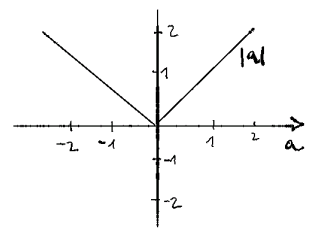
\includegraphics[width=0.4\textwidth]{betrag.png}
    \caption{Der Verlauf der $db_{FS}$ Kurve.}
    \label{fig:dbfs}
\end{figure}


\begin{figure}[h!]
    \centering
    %% Creator: Matplotlib, PGF backend
%%
%% To include the figure in your LaTeX document, write
%%   \input{<filename>.pgf}
%%
%% Make sure the required packages are loaded in your preamble
%%   \usepackage{pgf}
%%
%% Also ensure that all the required font packages are loaded; for instance,
%% the lmodern package is sometimes necessary when using math font.
%%   \usepackage{lmodern}
%%
%% Figures using additional raster images can only be included by \input if
%% they are in the same directory as the main LaTeX file. For loading figures
%% from other directories you can use the `import` package
%%   \usepackage{import}
%%
%% and then include the figures with
%%   \import{<path to file>}{<filename>.pgf}
%%
%% Matplotlib used the following preamble
%%   \def\mathdefault#1{#1}
%%   \everymath=\expandafter{\the\everymath\displaystyle}
%%   
%%   \usepackage{fontspec}
%%   \setmainfont{VeraSe.ttf}[Path=\detokenize{/usr/share/fonts/TTF/}]
%%   \setsansfont{DejaVuSans.ttf}[Path=\detokenize{/home/pl/miniconda3/lib/python3.12/site-packages/matplotlib/mpl-data/fonts/ttf/}]
%%   \setmonofont{DejaVuSansMono.ttf}[Path=\detokenize{/home/pl/miniconda3/lib/python3.12/site-packages/matplotlib/mpl-data/fonts/ttf/}]
%%   \makeatletter\@ifpackageloaded{underscore}{}{\usepackage[strings]{underscore}}\makeatother
%%
\begingroup%
\makeatletter%
\begin{pgfpicture}%
\pgfpathrectangle{\pgfpointorigin}{\pgfqpoint{6.340780in}{3.166819in}}%
\pgfusepath{use as bounding box, clip}%
\begin{pgfscope}%
\pgfsetbuttcap%
\pgfsetmiterjoin%
\definecolor{currentfill}{rgb}{1.000000,1.000000,1.000000}%
\pgfsetfillcolor{currentfill}%
\pgfsetlinewidth{0.000000pt}%
\definecolor{currentstroke}{rgb}{1.000000,1.000000,1.000000}%
\pgfsetstrokecolor{currentstroke}%
\pgfsetdash{}{0pt}%
\pgfpathmoveto{\pgfqpoint{0.000000in}{0.000000in}}%
\pgfpathlineto{\pgfqpoint{6.340780in}{0.000000in}}%
\pgfpathlineto{\pgfqpoint{6.340780in}{3.166819in}}%
\pgfpathlineto{\pgfqpoint{0.000000in}{3.166819in}}%
\pgfpathlineto{\pgfqpoint{0.000000in}{0.000000in}}%
\pgfpathclose%
\pgfusepath{fill}%
\end{pgfscope}%
\begin{pgfscope}%
\pgfsetbuttcap%
\pgfsetmiterjoin%
\definecolor{currentfill}{rgb}{1.000000,1.000000,1.000000}%
\pgfsetfillcolor{currentfill}%
\pgfsetlinewidth{0.000000pt}%
\definecolor{currentstroke}{rgb}{0.000000,0.000000,0.000000}%
\pgfsetstrokecolor{currentstroke}%
\pgfsetstrokeopacity{0.000000}%
\pgfsetdash{}{0pt}%
\pgfpathmoveto{\pgfqpoint{0.639049in}{0.548486in}}%
\pgfpathlineto{\pgfqpoint{3.104958in}{0.548486in}}%
\pgfpathlineto{\pgfqpoint{3.104958in}{2.858486in}}%
\pgfpathlineto{\pgfqpoint{0.639049in}{2.858486in}}%
\pgfpathlineto{\pgfqpoint{0.639049in}{0.548486in}}%
\pgfpathclose%
\pgfusepath{fill}%
\end{pgfscope}%
\begin{pgfscope}%
\pgfsetbuttcap%
\pgfsetroundjoin%
\definecolor{currentfill}{rgb}{0.000000,0.000000,0.000000}%
\pgfsetfillcolor{currentfill}%
\pgfsetlinewidth{0.803000pt}%
\definecolor{currentstroke}{rgb}{0.000000,0.000000,0.000000}%
\pgfsetstrokecolor{currentstroke}%
\pgfsetdash{}{0pt}%
\pgfsys@defobject{currentmarker}{\pgfqpoint{0.000000in}{-0.048611in}}{\pgfqpoint{0.000000in}{0.000000in}}{%
\pgfpathmoveto{\pgfqpoint{0.000000in}{0.000000in}}%
\pgfpathlineto{\pgfqpoint{0.000000in}{-0.048611in}}%
\pgfusepath{stroke,fill}%
}%
\begin{pgfscope}%
\pgfsys@transformshift{0.639049in}{0.548486in}%
\pgfsys@useobject{currentmarker}{}%
\end{pgfscope}%
\end{pgfscope}%
\begin{pgfscope}%
\definecolor{textcolor}{rgb}{0.000000,0.000000,0.000000}%
\pgfsetstrokecolor{textcolor}%
\pgfsetfillcolor{textcolor}%
\pgftext[x=0.639049in,y=0.451264in,,top]{\color{textcolor}{\rmfamily\fontsize{10.000000}{12.000000}\selectfont\catcode`\^=\active\def^{\ifmmode\sp\else\^{}\fi}\catcode`\%=\active\def%{\%}0}}%
\end{pgfscope}%
\begin{pgfscope}%
\pgfsetbuttcap%
\pgfsetroundjoin%
\definecolor{currentfill}{rgb}{0.000000,0.000000,0.000000}%
\pgfsetfillcolor{currentfill}%
\pgfsetlinewidth{0.803000pt}%
\definecolor{currentstroke}{rgb}{0.000000,0.000000,0.000000}%
\pgfsetstrokecolor{currentstroke}%
\pgfsetdash{}{0pt}%
\pgfsys@defobject{currentmarker}{\pgfqpoint{0.000000in}{-0.048611in}}{\pgfqpoint{0.000000in}{0.000000in}}{%
\pgfpathmoveto{\pgfqpoint{0.000000in}{0.000000in}}%
\pgfpathlineto{\pgfqpoint{0.000000in}{-0.048611in}}%
\pgfusepath{stroke,fill}%
}%
\begin{pgfscope}%
\pgfsys@transformshift{1.255526in}{0.548486in}%
\pgfsys@useobject{currentmarker}{}%
\end{pgfscope}%
\end{pgfscope}%
\begin{pgfscope}%
\definecolor{textcolor}{rgb}{0.000000,0.000000,0.000000}%
\pgfsetstrokecolor{textcolor}%
\pgfsetfillcolor{textcolor}%
\pgftext[x=1.255526in,y=0.451264in,,top]{\color{textcolor}{\rmfamily\fontsize{10.000000}{12.000000}\selectfont\catcode`\^=\active\def^{\ifmmode\sp\else\^{}\fi}\catcode`\%=\active\def%{\%}500}}%
\end{pgfscope}%
\begin{pgfscope}%
\pgfsetbuttcap%
\pgfsetroundjoin%
\definecolor{currentfill}{rgb}{0.000000,0.000000,0.000000}%
\pgfsetfillcolor{currentfill}%
\pgfsetlinewidth{0.803000pt}%
\definecolor{currentstroke}{rgb}{0.000000,0.000000,0.000000}%
\pgfsetstrokecolor{currentstroke}%
\pgfsetdash{}{0pt}%
\pgfsys@defobject{currentmarker}{\pgfqpoint{0.000000in}{-0.048611in}}{\pgfqpoint{0.000000in}{0.000000in}}{%
\pgfpathmoveto{\pgfqpoint{0.000000in}{0.000000in}}%
\pgfpathlineto{\pgfqpoint{0.000000in}{-0.048611in}}%
\pgfusepath{stroke,fill}%
}%
\begin{pgfscope}%
\pgfsys@transformshift{1.872003in}{0.548486in}%
\pgfsys@useobject{currentmarker}{}%
\end{pgfscope}%
\end{pgfscope}%
\begin{pgfscope}%
\definecolor{textcolor}{rgb}{0.000000,0.000000,0.000000}%
\pgfsetstrokecolor{textcolor}%
\pgfsetfillcolor{textcolor}%
\pgftext[x=1.872003in,y=0.451264in,,top]{\color{textcolor}{\rmfamily\fontsize{10.000000}{12.000000}\selectfont\catcode`\^=\active\def^{\ifmmode\sp\else\^{}\fi}\catcode`\%=\active\def%{\%}1000}}%
\end{pgfscope}%
\begin{pgfscope}%
\pgfsetbuttcap%
\pgfsetroundjoin%
\definecolor{currentfill}{rgb}{0.000000,0.000000,0.000000}%
\pgfsetfillcolor{currentfill}%
\pgfsetlinewidth{0.803000pt}%
\definecolor{currentstroke}{rgb}{0.000000,0.000000,0.000000}%
\pgfsetstrokecolor{currentstroke}%
\pgfsetdash{}{0pt}%
\pgfsys@defobject{currentmarker}{\pgfqpoint{0.000000in}{-0.048611in}}{\pgfqpoint{0.000000in}{0.000000in}}{%
\pgfpathmoveto{\pgfqpoint{0.000000in}{0.000000in}}%
\pgfpathlineto{\pgfqpoint{0.000000in}{-0.048611in}}%
\pgfusepath{stroke,fill}%
}%
\begin{pgfscope}%
\pgfsys@transformshift{2.488481in}{0.548486in}%
\pgfsys@useobject{currentmarker}{}%
\end{pgfscope}%
\end{pgfscope}%
\begin{pgfscope}%
\definecolor{textcolor}{rgb}{0.000000,0.000000,0.000000}%
\pgfsetstrokecolor{textcolor}%
\pgfsetfillcolor{textcolor}%
\pgftext[x=2.488481in,y=0.451264in,,top]{\color{textcolor}{\rmfamily\fontsize{10.000000}{12.000000}\selectfont\catcode`\^=\active\def^{\ifmmode\sp\else\^{}\fi}\catcode`\%=\active\def%{\%}1500}}%
\end{pgfscope}%
\begin{pgfscope}%
\pgfsetbuttcap%
\pgfsetroundjoin%
\definecolor{currentfill}{rgb}{0.000000,0.000000,0.000000}%
\pgfsetfillcolor{currentfill}%
\pgfsetlinewidth{0.803000pt}%
\definecolor{currentstroke}{rgb}{0.000000,0.000000,0.000000}%
\pgfsetstrokecolor{currentstroke}%
\pgfsetdash{}{0pt}%
\pgfsys@defobject{currentmarker}{\pgfqpoint{0.000000in}{-0.048611in}}{\pgfqpoint{0.000000in}{0.000000in}}{%
\pgfpathmoveto{\pgfqpoint{0.000000in}{0.000000in}}%
\pgfpathlineto{\pgfqpoint{0.000000in}{-0.048611in}}%
\pgfusepath{stroke,fill}%
}%
\begin{pgfscope}%
\pgfsys@transformshift{3.104958in}{0.548486in}%
\pgfsys@useobject{currentmarker}{}%
\end{pgfscope}%
\end{pgfscope}%
\begin{pgfscope}%
\definecolor{textcolor}{rgb}{0.000000,0.000000,0.000000}%
\pgfsetstrokecolor{textcolor}%
\pgfsetfillcolor{textcolor}%
\pgftext[x=3.104958in,y=0.451264in,,top]{\color{textcolor}{\rmfamily\fontsize{10.000000}{12.000000}\selectfont\catcode`\^=\active\def^{\ifmmode\sp\else\^{}\fi}\catcode`\%=\active\def%{\%}2000}}%
\end{pgfscope}%
\begin{pgfscope}%
\definecolor{textcolor}{rgb}{0.000000,0.000000,0.000000}%
\pgfsetstrokecolor{textcolor}%
\pgfsetfillcolor{textcolor}%
\pgftext[x=1.872003in,y=0.261295in,,top]{\color{textcolor}{\rmfamily\fontsize{12.000000}{14.400000}\selectfont\catcode`\^=\active\def^{\ifmmode\sp\else\^{}\fi}\catcode`\%=\active\def%{\%}f [Hz]}}%
\end{pgfscope}%
\begin{pgfscope}%
\pgfsetbuttcap%
\pgfsetroundjoin%
\definecolor{currentfill}{rgb}{0.000000,0.000000,0.000000}%
\pgfsetfillcolor{currentfill}%
\pgfsetlinewidth{0.803000pt}%
\definecolor{currentstroke}{rgb}{0.000000,0.000000,0.000000}%
\pgfsetstrokecolor{currentstroke}%
\pgfsetdash{}{0pt}%
\pgfsys@defobject{currentmarker}{\pgfqpoint{-0.048611in}{0.000000in}}{\pgfqpoint{-0.000000in}{0.000000in}}{%
\pgfpathmoveto{\pgfqpoint{-0.000000in}{0.000000in}}%
\pgfpathlineto{\pgfqpoint{-0.048611in}{0.000000in}}%
\pgfusepath{stroke,fill}%
}%
\begin{pgfscope}%
\pgfsys@transformshift{0.639049in}{1.010485in}%
\pgfsys@useobject{currentmarker}{}%
\end{pgfscope}%
\end{pgfscope}%
\begin{pgfscope}%
\definecolor{textcolor}{rgb}{0.000000,0.000000,0.000000}%
\pgfsetstrokecolor{textcolor}%
\pgfsetfillcolor{textcolor}%
\pgftext[x=0.188365in, y=0.957724in, left, base]{\color{textcolor}{\rmfamily\fontsize{10.000000}{12.000000}\selectfont\catcode`\^=\active\def^{\ifmmode\sp\else\^{}\fi}\catcode`\%=\active\def%{\%}2000}}%
\end{pgfscope}%
\begin{pgfscope}%
\pgfsetbuttcap%
\pgfsetroundjoin%
\definecolor{currentfill}{rgb}{0.000000,0.000000,0.000000}%
\pgfsetfillcolor{currentfill}%
\pgfsetlinewidth{0.803000pt}%
\definecolor{currentstroke}{rgb}{0.000000,0.000000,0.000000}%
\pgfsetstrokecolor{currentstroke}%
\pgfsetdash{}{0pt}%
\pgfsys@defobject{currentmarker}{\pgfqpoint{-0.048611in}{0.000000in}}{\pgfqpoint{-0.000000in}{0.000000in}}{%
\pgfpathmoveto{\pgfqpoint{-0.000000in}{0.000000in}}%
\pgfpathlineto{\pgfqpoint{-0.048611in}{0.000000in}}%
\pgfusepath{stroke,fill}%
}%
\begin{pgfscope}%
\pgfsys@transformshift{0.639049in}{1.472486in}%
\pgfsys@useobject{currentmarker}{}%
\end{pgfscope}%
\end{pgfscope}%
\begin{pgfscope}%
\definecolor{textcolor}{rgb}{0.000000,0.000000,0.000000}%
\pgfsetstrokecolor{textcolor}%
\pgfsetfillcolor{textcolor}%
\pgftext[x=0.188365in, y=1.419724in, left, base]{\color{textcolor}{\rmfamily\fontsize{10.000000}{12.000000}\selectfont\catcode`\^=\active\def^{\ifmmode\sp\else\^{}\fi}\catcode`\%=\active\def%{\%}4000}}%
\end{pgfscope}%
\begin{pgfscope}%
\pgfsetbuttcap%
\pgfsetroundjoin%
\definecolor{currentfill}{rgb}{0.000000,0.000000,0.000000}%
\pgfsetfillcolor{currentfill}%
\pgfsetlinewidth{0.803000pt}%
\definecolor{currentstroke}{rgb}{0.000000,0.000000,0.000000}%
\pgfsetstrokecolor{currentstroke}%
\pgfsetdash{}{0pt}%
\pgfsys@defobject{currentmarker}{\pgfqpoint{-0.048611in}{0.000000in}}{\pgfqpoint{-0.000000in}{0.000000in}}{%
\pgfpathmoveto{\pgfqpoint{-0.000000in}{0.000000in}}%
\pgfpathlineto{\pgfqpoint{-0.048611in}{0.000000in}}%
\pgfusepath{stroke,fill}%
}%
\begin{pgfscope}%
\pgfsys@transformshift{0.639049in}{1.934486in}%
\pgfsys@useobject{currentmarker}{}%
\end{pgfscope}%
\end{pgfscope}%
\begin{pgfscope}%
\definecolor{textcolor}{rgb}{0.000000,0.000000,0.000000}%
\pgfsetstrokecolor{textcolor}%
\pgfsetfillcolor{textcolor}%
\pgftext[x=0.188365in, y=1.881724in, left, base]{\color{textcolor}{\rmfamily\fontsize{10.000000}{12.000000}\selectfont\catcode`\^=\active\def^{\ifmmode\sp\else\^{}\fi}\catcode`\%=\active\def%{\%}6000}}%
\end{pgfscope}%
\begin{pgfscope}%
\pgfsetbuttcap%
\pgfsetroundjoin%
\definecolor{currentfill}{rgb}{0.000000,0.000000,0.000000}%
\pgfsetfillcolor{currentfill}%
\pgfsetlinewidth{0.803000pt}%
\definecolor{currentstroke}{rgb}{0.000000,0.000000,0.000000}%
\pgfsetstrokecolor{currentstroke}%
\pgfsetdash{}{0pt}%
\pgfsys@defobject{currentmarker}{\pgfqpoint{-0.048611in}{0.000000in}}{\pgfqpoint{-0.000000in}{0.000000in}}{%
\pgfpathmoveto{\pgfqpoint{-0.000000in}{0.000000in}}%
\pgfpathlineto{\pgfqpoint{-0.048611in}{0.000000in}}%
\pgfusepath{stroke,fill}%
}%
\begin{pgfscope}%
\pgfsys@transformshift{0.639049in}{2.396486in}%
\pgfsys@useobject{currentmarker}{}%
\end{pgfscope}%
\end{pgfscope}%
\begin{pgfscope}%
\definecolor{textcolor}{rgb}{0.000000,0.000000,0.000000}%
\pgfsetstrokecolor{textcolor}%
\pgfsetfillcolor{textcolor}%
\pgftext[x=0.188365in, y=2.343724in, left, base]{\color{textcolor}{\rmfamily\fontsize{10.000000}{12.000000}\selectfont\catcode`\^=\active\def^{\ifmmode\sp\else\^{}\fi}\catcode`\%=\active\def%{\%}8000}}%
\end{pgfscope}%
\begin{pgfscope}%
\pgfsetbuttcap%
\pgfsetroundjoin%
\definecolor{currentfill}{rgb}{0.000000,0.000000,0.000000}%
\pgfsetfillcolor{currentfill}%
\pgfsetlinewidth{0.803000pt}%
\definecolor{currentstroke}{rgb}{0.000000,0.000000,0.000000}%
\pgfsetstrokecolor{currentstroke}%
\pgfsetdash{}{0pt}%
\pgfsys@defobject{currentmarker}{\pgfqpoint{-0.048611in}{0.000000in}}{\pgfqpoint{-0.000000in}{0.000000in}}{%
\pgfpathmoveto{\pgfqpoint{-0.000000in}{0.000000in}}%
\pgfpathlineto{\pgfqpoint{-0.048611in}{0.000000in}}%
\pgfusepath{stroke,fill}%
}%
\begin{pgfscope}%
\pgfsys@transformshift{0.639049in}{2.858486in}%
\pgfsys@useobject{currentmarker}{}%
\end{pgfscope}%
\end{pgfscope}%
\begin{pgfscope}%
\definecolor{textcolor}{rgb}{0.000000,0.000000,0.000000}%
\pgfsetstrokecolor{textcolor}%
\pgfsetfillcolor{textcolor}%
\pgftext[x=0.100000in, y=2.805724in, left, base]{\color{textcolor}{\rmfamily\fontsize{10.000000}{12.000000}\selectfont\catcode`\^=\active\def^{\ifmmode\sp\else\^{}\fi}\catcode`\%=\active\def%{\%}10000}}%
\end{pgfscope}%
\begin{pgfscope}%
\pgfpathrectangle{\pgfqpoint{0.639049in}{0.548486in}}{\pgfqpoint{2.465909in}{2.310000in}}%
\pgfusepath{clip}%
\pgfsetrectcap%
\pgfsetroundjoin%
\pgfsetlinewidth{1.505625pt}%
\definecolor{currentstroke}{rgb}{0.000000,0.000000,0.000000}%
\pgfsetstrokecolor{currentstroke}%
\pgfsetdash{}{0pt}%
\pgfpathmoveto{\pgfqpoint{0.637816in}{0.548488in}}%
\pgfpathlineto{\pgfqpoint{0.742617in}{0.549304in}}%
\pgfpathlineto{\pgfqpoint{0.754947in}{0.550755in}}%
\pgfpathlineto{\pgfqpoint{0.758645in}{0.553054in}}%
\pgfpathlineto{\pgfqpoint{0.759878in}{0.555334in}}%
\pgfpathlineto{\pgfqpoint{0.761111in}{0.562072in}}%
\pgfpathlineto{\pgfqpoint{0.762344in}{1.162913in}}%
\pgfpathlineto{\pgfqpoint{0.763577in}{0.562784in}}%
\pgfpathlineto{\pgfqpoint{0.766043in}{0.553204in}}%
\pgfpathlineto{\pgfqpoint{0.769742in}{0.550852in}}%
\pgfpathlineto{\pgfqpoint{0.778373in}{0.549590in}}%
\pgfpathlineto{\pgfqpoint{0.806731in}{0.548887in}}%
\pgfpathlineto{\pgfqpoint{0.959617in}{0.548605in}}%
\pgfpathlineto{\pgfqpoint{1.000305in}{0.549766in}}%
\pgfpathlineto{\pgfqpoint{1.005236in}{0.551571in}}%
\pgfpathlineto{\pgfqpoint{1.006469in}{0.553111in}}%
\pgfpathlineto{\pgfqpoint{1.007702in}{0.557535in}}%
\pgfpathlineto{\pgfqpoint{1.008935in}{0.691956in}}%
\pgfpathlineto{\pgfqpoint{1.010168in}{0.559063in}}%
\pgfpathlineto{\pgfqpoint{1.012634in}{0.551912in}}%
\pgfpathlineto{\pgfqpoint{1.016333in}{0.550225in}}%
\pgfpathlineto{\pgfqpoint{1.026197in}{0.549274in}}%
\pgfpathlineto{\pgfqpoint{1.068117in}{0.548757in}}%
\pgfpathlineto{\pgfqpoint{1.246895in}{0.549144in}}%
\pgfpathlineto{\pgfqpoint{1.251827in}{0.550142in}}%
\pgfpathlineto{\pgfqpoint{1.253060in}{0.550980in}}%
\pgfpathlineto{\pgfqpoint{1.254293in}{0.553324in}}%
\pgfpathlineto{\pgfqpoint{1.255526in}{0.596997in}}%
\pgfpathlineto{\pgfqpoint{1.256759in}{0.554818in}}%
\pgfpathlineto{\pgfqpoint{1.259225in}{0.550507in}}%
\pgfpathlineto{\pgfqpoint{1.264157in}{0.549396in}}%
\pgfpathlineto{\pgfqpoint{1.283884in}{0.548829in}}%
\pgfpathlineto{\pgfqpoint{1.446634in}{0.548547in}}%
\pgfpathlineto{\pgfqpoint{1.498418in}{0.549243in}}%
\pgfpathlineto{\pgfqpoint{1.500884in}{0.550738in}}%
\pgfpathlineto{\pgfqpoint{1.502117in}{0.565599in}}%
\pgfpathlineto{\pgfqpoint{1.504583in}{0.550076in}}%
\pgfpathlineto{\pgfqpoint{1.509515in}{0.549058in}}%
\pgfpathlineto{\pgfqpoint{1.535407in}{0.548686in}}%
\pgfpathlineto{\pgfqpoint{1.746242in}{0.548959in}}%
\pgfpathlineto{\pgfqpoint{1.747475in}{0.549430in}}%
\pgfpathlineto{\pgfqpoint{1.748708in}{0.554510in}}%
\pgfpathlineto{\pgfqpoint{1.751174in}{0.549272in}}%
\pgfpathlineto{\pgfqpoint{1.758572in}{0.548736in}}%
\pgfpathlineto{\pgfqpoint{1.842413in}{0.548582in}}%
\pgfpathlineto{\pgfqpoint{1.994066in}{0.548838in}}%
\pgfpathlineto{\pgfqpoint{1.995299in}{0.550568in}}%
\pgfpathlineto{\pgfqpoint{1.997765in}{0.548872in}}%
\pgfpathlineto{\pgfqpoint{2.012560in}{0.548602in}}%
\pgfpathlineto{\pgfqpoint{2.487248in}{0.548491in}}%
\pgfpathlineto{\pgfqpoint{2.494645in}{0.548565in}}%
\pgfpathlineto{\pgfqpoint{2.901520in}{0.548539in}}%
\pgfpathlineto{\pgfqpoint{3.106191in}{0.548537in}}%
\pgfpathlineto{\pgfqpoint{3.106191in}{0.548537in}}%
\pgfusepath{stroke}%
\end{pgfscope}%
\begin{pgfscope}%
\definecolor{textcolor}{rgb}{0.000000,0.000000,0.000000}%
\pgfsetstrokecolor{textcolor}%
\pgfsetfillcolor{textcolor}%
\pgftext[x=1.872003in,y=2.941819in,,base]{\color{textcolor}{\rmfamily\fontsize{12.000000}{14.400000}\selectfont\catcode`\^=\active\def^{\ifmmode\sp\else\^{}\fi}\catcode`\%=\active\def%{\%}$|X(f)|$}}%
\end{pgfscope}%
\begin{pgfscope}%
\pgfsetbuttcap%
\pgfsetmiterjoin%
\definecolor{currentfill}{rgb}{1.000000,1.000000,1.000000}%
\pgfsetfillcolor{currentfill}%
\pgfsetlinewidth{0.000000pt}%
\definecolor{currentstroke}{rgb}{0.000000,0.000000,0.000000}%
\pgfsetstrokecolor{currentstroke}%
\pgfsetstrokeopacity{0.000000}%
\pgfsetdash{}{0pt}%
\pgfpathmoveto{\pgfqpoint{3.598140in}{0.548486in}}%
\pgfpathlineto{\pgfqpoint{6.064049in}{0.548486in}}%
\pgfpathlineto{\pgfqpoint{6.064049in}{2.858486in}}%
\pgfpathlineto{\pgfqpoint{3.598140in}{2.858486in}}%
\pgfpathlineto{\pgfqpoint{3.598140in}{0.548486in}}%
\pgfpathclose%
\pgfusepath{fill}%
\end{pgfscope}%
\begin{pgfscope}%
\pgfsetbuttcap%
\pgfsetroundjoin%
\definecolor{currentfill}{rgb}{0.000000,0.000000,0.000000}%
\pgfsetfillcolor{currentfill}%
\pgfsetlinewidth{0.803000pt}%
\definecolor{currentstroke}{rgb}{0.000000,0.000000,0.000000}%
\pgfsetstrokecolor{currentstroke}%
\pgfsetdash{}{0pt}%
\pgfsys@defobject{currentmarker}{\pgfqpoint{0.000000in}{-0.048611in}}{\pgfqpoint{0.000000in}{0.000000in}}{%
\pgfpathmoveto{\pgfqpoint{0.000000in}{0.000000in}}%
\pgfpathlineto{\pgfqpoint{0.000000in}{-0.048611in}}%
\pgfusepath{stroke,fill}%
}%
\begin{pgfscope}%
\pgfsys@transformshift{3.598140in}{0.548486in}%
\pgfsys@useobject{currentmarker}{}%
\end{pgfscope}%
\end{pgfscope}%
\begin{pgfscope}%
\definecolor{textcolor}{rgb}{0.000000,0.000000,0.000000}%
\pgfsetstrokecolor{textcolor}%
\pgfsetfillcolor{textcolor}%
\pgftext[x=3.598140in,y=0.451264in,,top]{\color{textcolor}{\rmfamily\fontsize{10.000000}{12.000000}\selectfont\catcode`\^=\active\def^{\ifmmode\sp\else\^{}\fi}\catcode`\%=\active\def%{\%}0}}%
\end{pgfscope}%
\begin{pgfscope}%
\pgfsetbuttcap%
\pgfsetroundjoin%
\definecolor{currentfill}{rgb}{0.000000,0.000000,0.000000}%
\pgfsetfillcolor{currentfill}%
\pgfsetlinewidth{0.803000pt}%
\definecolor{currentstroke}{rgb}{0.000000,0.000000,0.000000}%
\pgfsetstrokecolor{currentstroke}%
\pgfsetdash{}{0pt}%
\pgfsys@defobject{currentmarker}{\pgfqpoint{0.000000in}{-0.048611in}}{\pgfqpoint{0.000000in}{0.000000in}}{%
\pgfpathmoveto{\pgfqpoint{0.000000in}{0.000000in}}%
\pgfpathlineto{\pgfqpoint{0.000000in}{-0.048611in}}%
\pgfusepath{stroke,fill}%
}%
\begin{pgfscope}%
\pgfsys@transformshift{4.214617in}{0.548486in}%
\pgfsys@useobject{currentmarker}{}%
\end{pgfscope}%
\end{pgfscope}%
\begin{pgfscope}%
\definecolor{textcolor}{rgb}{0.000000,0.000000,0.000000}%
\pgfsetstrokecolor{textcolor}%
\pgfsetfillcolor{textcolor}%
\pgftext[x=4.214617in,y=0.451264in,,top]{\color{textcolor}{\rmfamily\fontsize{10.000000}{12.000000}\selectfont\catcode`\^=\active\def^{\ifmmode\sp\else\^{}\fi}\catcode`\%=\active\def%{\%}500}}%
\end{pgfscope}%
\begin{pgfscope}%
\pgfsetbuttcap%
\pgfsetroundjoin%
\definecolor{currentfill}{rgb}{0.000000,0.000000,0.000000}%
\pgfsetfillcolor{currentfill}%
\pgfsetlinewidth{0.803000pt}%
\definecolor{currentstroke}{rgb}{0.000000,0.000000,0.000000}%
\pgfsetstrokecolor{currentstroke}%
\pgfsetdash{}{0pt}%
\pgfsys@defobject{currentmarker}{\pgfqpoint{0.000000in}{-0.048611in}}{\pgfqpoint{0.000000in}{0.000000in}}{%
\pgfpathmoveto{\pgfqpoint{0.000000in}{0.000000in}}%
\pgfpathlineto{\pgfqpoint{0.000000in}{-0.048611in}}%
\pgfusepath{stroke,fill}%
}%
\begin{pgfscope}%
\pgfsys@transformshift{4.831094in}{0.548486in}%
\pgfsys@useobject{currentmarker}{}%
\end{pgfscope}%
\end{pgfscope}%
\begin{pgfscope}%
\definecolor{textcolor}{rgb}{0.000000,0.000000,0.000000}%
\pgfsetstrokecolor{textcolor}%
\pgfsetfillcolor{textcolor}%
\pgftext[x=4.831094in,y=0.451264in,,top]{\color{textcolor}{\rmfamily\fontsize{10.000000}{12.000000}\selectfont\catcode`\^=\active\def^{\ifmmode\sp\else\^{}\fi}\catcode`\%=\active\def%{\%}1000}}%
\end{pgfscope}%
\begin{pgfscope}%
\pgfsetbuttcap%
\pgfsetroundjoin%
\definecolor{currentfill}{rgb}{0.000000,0.000000,0.000000}%
\pgfsetfillcolor{currentfill}%
\pgfsetlinewidth{0.803000pt}%
\definecolor{currentstroke}{rgb}{0.000000,0.000000,0.000000}%
\pgfsetstrokecolor{currentstroke}%
\pgfsetdash{}{0pt}%
\pgfsys@defobject{currentmarker}{\pgfqpoint{0.000000in}{-0.048611in}}{\pgfqpoint{0.000000in}{0.000000in}}{%
\pgfpathmoveto{\pgfqpoint{0.000000in}{0.000000in}}%
\pgfpathlineto{\pgfqpoint{0.000000in}{-0.048611in}}%
\pgfusepath{stroke,fill}%
}%
\begin{pgfscope}%
\pgfsys@transformshift{5.447572in}{0.548486in}%
\pgfsys@useobject{currentmarker}{}%
\end{pgfscope}%
\end{pgfscope}%
\begin{pgfscope}%
\definecolor{textcolor}{rgb}{0.000000,0.000000,0.000000}%
\pgfsetstrokecolor{textcolor}%
\pgfsetfillcolor{textcolor}%
\pgftext[x=5.447572in,y=0.451264in,,top]{\color{textcolor}{\rmfamily\fontsize{10.000000}{12.000000}\selectfont\catcode`\^=\active\def^{\ifmmode\sp\else\^{}\fi}\catcode`\%=\active\def%{\%}1500}}%
\end{pgfscope}%
\begin{pgfscope}%
\pgfsetbuttcap%
\pgfsetroundjoin%
\definecolor{currentfill}{rgb}{0.000000,0.000000,0.000000}%
\pgfsetfillcolor{currentfill}%
\pgfsetlinewidth{0.803000pt}%
\definecolor{currentstroke}{rgb}{0.000000,0.000000,0.000000}%
\pgfsetstrokecolor{currentstroke}%
\pgfsetdash{}{0pt}%
\pgfsys@defobject{currentmarker}{\pgfqpoint{0.000000in}{-0.048611in}}{\pgfqpoint{0.000000in}{0.000000in}}{%
\pgfpathmoveto{\pgfqpoint{0.000000in}{0.000000in}}%
\pgfpathlineto{\pgfqpoint{0.000000in}{-0.048611in}}%
\pgfusepath{stroke,fill}%
}%
\begin{pgfscope}%
\pgfsys@transformshift{6.064049in}{0.548486in}%
\pgfsys@useobject{currentmarker}{}%
\end{pgfscope}%
\end{pgfscope}%
\begin{pgfscope}%
\definecolor{textcolor}{rgb}{0.000000,0.000000,0.000000}%
\pgfsetstrokecolor{textcolor}%
\pgfsetfillcolor{textcolor}%
\pgftext[x=6.064049in,y=0.451264in,,top]{\color{textcolor}{\rmfamily\fontsize{10.000000}{12.000000}\selectfont\catcode`\^=\active\def^{\ifmmode\sp\else\^{}\fi}\catcode`\%=\active\def%{\%}2000}}%
\end{pgfscope}%
\begin{pgfscope}%
\definecolor{textcolor}{rgb}{0.000000,0.000000,0.000000}%
\pgfsetstrokecolor{textcolor}%
\pgfsetfillcolor{textcolor}%
\pgftext[x=4.831094in,y=0.261295in,,top]{\color{textcolor}{\rmfamily\fontsize{12.000000}{14.400000}\selectfont\catcode`\^=\active\def^{\ifmmode\sp\else\^{}\fi}\catcode`\%=\active\def%{\%}f [Hz]}}%
\end{pgfscope}%
\begin{pgfscope}%
\pgfsetbuttcap%
\pgfsetroundjoin%
\definecolor{currentfill}{rgb}{0.000000,0.000000,0.000000}%
\pgfsetfillcolor{currentfill}%
\pgfsetlinewidth{0.803000pt}%
\definecolor{currentstroke}{rgb}{0.000000,0.000000,0.000000}%
\pgfsetstrokecolor{currentstroke}%
\pgfsetdash{}{0pt}%
\pgfsys@defobject{currentmarker}{\pgfqpoint{-0.048611in}{0.000000in}}{\pgfqpoint{-0.000000in}{0.000000in}}{%
\pgfpathmoveto{\pgfqpoint{-0.000000in}{0.000000in}}%
\pgfpathlineto{\pgfqpoint{-0.048611in}{0.000000in}}%
\pgfusepath{stroke,fill}%
}%
\begin{pgfscope}%
\pgfsys@transformshift{3.598140in}{0.726178in}%
\pgfsys@useobject{currentmarker}{}%
\end{pgfscope}%
\end{pgfscope}%
\begin{pgfscope}%
\definecolor{textcolor}{rgb}{0.000000,0.000000,0.000000}%
\pgfsetstrokecolor{textcolor}%
\pgfsetfillcolor{textcolor}%
\pgftext[x=3.216162in, y=0.673417in, left, base]{\color{textcolor}{\rmfamily\fontsize{10.000000}{12.000000}\selectfont\catcode`\^=\active\def^{\ifmmode\sp\else\^{}\fi}\catcode`\%=\active\def%{\%}\ensuremath{-}40}}%
\end{pgfscope}%
\begin{pgfscope}%
\pgfsetbuttcap%
\pgfsetroundjoin%
\definecolor{currentfill}{rgb}{0.000000,0.000000,0.000000}%
\pgfsetfillcolor{currentfill}%
\pgfsetlinewidth{0.803000pt}%
\definecolor{currentstroke}{rgb}{0.000000,0.000000,0.000000}%
\pgfsetstrokecolor{currentstroke}%
\pgfsetdash{}{0pt}%
\pgfsys@defobject{currentmarker}{\pgfqpoint{-0.048611in}{0.000000in}}{\pgfqpoint{-0.000000in}{0.000000in}}{%
\pgfpathmoveto{\pgfqpoint{-0.000000in}{0.000000in}}%
\pgfpathlineto{\pgfqpoint{-0.048611in}{0.000000in}}%
\pgfusepath{stroke,fill}%
}%
\begin{pgfscope}%
\pgfsys@transformshift{3.598140in}{1.081563in}%
\pgfsys@useobject{currentmarker}{}%
\end{pgfscope}%
\end{pgfscope}%
\begin{pgfscope}%
\definecolor{textcolor}{rgb}{0.000000,0.000000,0.000000}%
\pgfsetstrokecolor{textcolor}%
\pgfsetfillcolor{textcolor}%
\pgftext[x=3.216162in, y=1.028801in, left, base]{\color{textcolor}{\rmfamily\fontsize{10.000000}{12.000000}\selectfont\catcode`\^=\active\def^{\ifmmode\sp\else\^{}\fi}\catcode`\%=\active\def%{\%}\ensuremath{-}20}}%
\end{pgfscope}%
\begin{pgfscope}%
\pgfsetbuttcap%
\pgfsetroundjoin%
\definecolor{currentfill}{rgb}{0.000000,0.000000,0.000000}%
\pgfsetfillcolor{currentfill}%
\pgfsetlinewidth{0.803000pt}%
\definecolor{currentstroke}{rgb}{0.000000,0.000000,0.000000}%
\pgfsetstrokecolor{currentstroke}%
\pgfsetdash{}{0pt}%
\pgfsys@defobject{currentmarker}{\pgfqpoint{-0.048611in}{0.000000in}}{\pgfqpoint{-0.000000in}{0.000000in}}{%
\pgfpathmoveto{\pgfqpoint{-0.000000in}{0.000000in}}%
\pgfpathlineto{\pgfqpoint{-0.048611in}{0.000000in}}%
\pgfusepath{stroke,fill}%
}%
\begin{pgfscope}%
\pgfsys@transformshift{3.598140in}{1.436948in}%
\pgfsys@useobject{currentmarker}{}%
\end{pgfscope}%
\end{pgfscope}%
\begin{pgfscope}%
\definecolor{textcolor}{rgb}{0.000000,0.000000,0.000000}%
\pgfsetstrokecolor{textcolor}%
\pgfsetfillcolor{textcolor}%
\pgftext[x=3.412552in, y=1.384186in, left, base]{\color{textcolor}{\rmfamily\fontsize{10.000000}{12.000000}\selectfont\catcode`\^=\active\def^{\ifmmode\sp\else\^{}\fi}\catcode`\%=\active\def%{\%}0}}%
\end{pgfscope}%
\begin{pgfscope}%
\pgfsetbuttcap%
\pgfsetroundjoin%
\definecolor{currentfill}{rgb}{0.000000,0.000000,0.000000}%
\pgfsetfillcolor{currentfill}%
\pgfsetlinewidth{0.803000pt}%
\definecolor{currentstroke}{rgb}{0.000000,0.000000,0.000000}%
\pgfsetstrokecolor{currentstroke}%
\pgfsetdash{}{0pt}%
\pgfsys@defobject{currentmarker}{\pgfqpoint{-0.048611in}{0.000000in}}{\pgfqpoint{-0.000000in}{0.000000in}}{%
\pgfpathmoveto{\pgfqpoint{-0.000000in}{0.000000in}}%
\pgfpathlineto{\pgfqpoint{-0.048611in}{0.000000in}}%
\pgfusepath{stroke,fill}%
}%
\begin{pgfscope}%
\pgfsys@transformshift{3.598140in}{1.792332in}%
\pgfsys@useobject{currentmarker}{}%
\end{pgfscope}%
\end{pgfscope}%
\begin{pgfscope}%
\definecolor{textcolor}{rgb}{0.000000,0.000000,0.000000}%
\pgfsetstrokecolor{textcolor}%
\pgfsetfillcolor{textcolor}%
\pgftext[x=3.324187in, y=1.739571in, left, base]{\color{textcolor}{\rmfamily\fontsize{10.000000}{12.000000}\selectfont\catcode`\^=\active\def^{\ifmmode\sp\else\^{}\fi}\catcode`\%=\active\def%{\%}20}}%
\end{pgfscope}%
\begin{pgfscope}%
\pgfsetbuttcap%
\pgfsetroundjoin%
\definecolor{currentfill}{rgb}{0.000000,0.000000,0.000000}%
\pgfsetfillcolor{currentfill}%
\pgfsetlinewidth{0.803000pt}%
\definecolor{currentstroke}{rgb}{0.000000,0.000000,0.000000}%
\pgfsetstrokecolor{currentstroke}%
\pgfsetdash{}{0pt}%
\pgfsys@defobject{currentmarker}{\pgfqpoint{-0.048611in}{0.000000in}}{\pgfqpoint{-0.000000in}{0.000000in}}{%
\pgfpathmoveto{\pgfqpoint{-0.000000in}{0.000000in}}%
\pgfpathlineto{\pgfqpoint{-0.048611in}{0.000000in}}%
\pgfusepath{stroke,fill}%
}%
\begin{pgfscope}%
\pgfsys@transformshift{3.598140in}{2.147717in}%
\pgfsys@useobject{currentmarker}{}%
\end{pgfscope}%
\end{pgfscope}%
\begin{pgfscope}%
\definecolor{textcolor}{rgb}{0.000000,0.000000,0.000000}%
\pgfsetstrokecolor{textcolor}%
\pgfsetfillcolor{textcolor}%
\pgftext[x=3.324187in, y=2.094955in, left, base]{\color{textcolor}{\rmfamily\fontsize{10.000000}{12.000000}\selectfont\catcode`\^=\active\def^{\ifmmode\sp\else\^{}\fi}\catcode`\%=\active\def%{\%}40}}%
\end{pgfscope}%
\begin{pgfscope}%
\pgfsetbuttcap%
\pgfsetroundjoin%
\definecolor{currentfill}{rgb}{0.000000,0.000000,0.000000}%
\pgfsetfillcolor{currentfill}%
\pgfsetlinewidth{0.803000pt}%
\definecolor{currentstroke}{rgb}{0.000000,0.000000,0.000000}%
\pgfsetstrokecolor{currentstroke}%
\pgfsetdash{}{0pt}%
\pgfsys@defobject{currentmarker}{\pgfqpoint{-0.048611in}{0.000000in}}{\pgfqpoint{-0.000000in}{0.000000in}}{%
\pgfpathmoveto{\pgfqpoint{-0.000000in}{0.000000in}}%
\pgfpathlineto{\pgfqpoint{-0.048611in}{0.000000in}}%
\pgfusepath{stroke,fill}%
}%
\begin{pgfscope}%
\pgfsys@transformshift{3.598140in}{2.503101in}%
\pgfsys@useobject{currentmarker}{}%
\end{pgfscope}%
\end{pgfscope}%
\begin{pgfscope}%
\definecolor{textcolor}{rgb}{0.000000,0.000000,0.000000}%
\pgfsetstrokecolor{textcolor}%
\pgfsetfillcolor{textcolor}%
\pgftext[x=3.324187in, y=2.450340in, left, base]{\color{textcolor}{\rmfamily\fontsize{10.000000}{12.000000}\selectfont\catcode`\^=\active\def^{\ifmmode\sp\else\^{}\fi}\catcode`\%=\active\def%{\%}60}}%
\end{pgfscope}%
\begin{pgfscope}%
\pgfsetbuttcap%
\pgfsetroundjoin%
\definecolor{currentfill}{rgb}{0.000000,0.000000,0.000000}%
\pgfsetfillcolor{currentfill}%
\pgfsetlinewidth{0.803000pt}%
\definecolor{currentstroke}{rgb}{0.000000,0.000000,0.000000}%
\pgfsetstrokecolor{currentstroke}%
\pgfsetdash{}{0pt}%
\pgfsys@defobject{currentmarker}{\pgfqpoint{-0.048611in}{0.000000in}}{\pgfqpoint{-0.000000in}{0.000000in}}{%
\pgfpathmoveto{\pgfqpoint{-0.000000in}{0.000000in}}%
\pgfpathlineto{\pgfqpoint{-0.048611in}{0.000000in}}%
\pgfusepath{stroke,fill}%
}%
\begin{pgfscope}%
\pgfsys@transformshift{3.598140in}{2.858486in}%
\pgfsys@useobject{currentmarker}{}%
\end{pgfscope}%
\end{pgfscope}%
\begin{pgfscope}%
\definecolor{textcolor}{rgb}{0.000000,0.000000,0.000000}%
\pgfsetstrokecolor{textcolor}%
\pgfsetfillcolor{textcolor}%
\pgftext[x=3.324187in, y=2.805724in, left, base]{\color{textcolor}{\rmfamily\fontsize{10.000000}{12.000000}\selectfont\catcode`\^=\active\def^{\ifmmode\sp\else\^{}\fi}\catcode`\%=\active\def%{\%}80}}%
\end{pgfscope}%
\begin{pgfscope}%
\pgfpathrectangle{\pgfqpoint{3.598140in}{0.548486in}}{\pgfqpoint{2.465909in}{2.310000in}}%
\pgfusepath{clip}%
\pgfsetrectcap%
\pgfsetroundjoin%
\pgfsetlinewidth{1.505625pt}%
\definecolor{currentstroke}{rgb}{0.000000,0.000000,0.000000}%
\pgfsetstrokecolor{currentstroke}%
\pgfsetdash{}{0pt}%
\pgfpathmoveto{\pgfqpoint{3.596907in}{0.769421in}}%
\pgfpathlineto{\pgfqpoint{3.596991in}{0.538486in}}%
\pgfpathmoveto{\pgfqpoint{3.599288in}{0.538486in}}%
\pgfpathlineto{\pgfqpoint{3.599373in}{0.769421in}}%
\pgfpathlineto{\pgfqpoint{3.601839in}{0.939096in}}%
\pgfpathlineto{\pgfqpoint{3.605538in}{1.046462in}}%
\pgfpathlineto{\pgfqpoint{3.610469in}{1.126218in}}%
\pgfpathlineto{\pgfqpoint{3.616634in}{1.190604in}}%
\pgfpathlineto{\pgfqpoint{3.624032in}{1.245714in}}%
\pgfpathlineto{\pgfqpoint{3.633895in}{1.301623in}}%
\pgfpathlineto{\pgfqpoint{3.646225in}{1.358383in}}%
\pgfpathlineto{\pgfqpoint{3.686913in}{1.535284in}}%
\pgfpathlineto{\pgfqpoint{3.695543in}{1.586273in}}%
\pgfpathlineto{\pgfqpoint{3.702941in}{1.642875in}}%
\pgfpathlineto{\pgfqpoint{3.709106in}{1.708696in}}%
\pgfpathlineto{\pgfqpoint{3.714038in}{1.789638in}}%
\pgfpathlineto{\pgfqpoint{3.717736in}{1.897596in}}%
\pgfpathlineto{\pgfqpoint{3.720202in}{2.065807in}}%
\pgfpathlineto{\pgfqpoint{3.721435in}{2.654090in}}%
\pgfpathlineto{\pgfqpoint{3.723901in}{1.965341in}}%
\pgfpathlineto{\pgfqpoint{3.727600in}{1.824004in}}%
\pgfpathlineto{\pgfqpoint{3.732532in}{1.734269in}}%
\pgfpathlineto{\pgfqpoint{3.738697in}{1.667202in}}%
\pgfpathlineto{\pgfqpoint{3.746094in}{1.613085in}}%
\pgfpathlineto{\pgfqpoint{3.754725in}{1.567196in}}%
\pgfpathlineto{\pgfqpoint{3.764589in}{1.526716in}}%
\pgfpathlineto{\pgfqpoint{3.776918in}{1.485912in}}%
\pgfpathlineto{\pgfqpoint{3.792947in}{1.441296in}}%
\pgfpathlineto{\pgfqpoint{3.839799in}{1.316444in}}%
\pgfpathlineto{\pgfqpoint{3.850895in}{1.277025in}}%
\pgfpathlineto{\pgfqpoint{3.859526in}{1.237829in}}%
\pgfpathlineto{\pgfqpoint{3.866924in}{1.192898in}}%
\pgfpathlineto{\pgfqpoint{3.873089in}{1.139674in}}%
\pgfpathlineto{\pgfqpoint{3.878020in}{1.074674in}}%
\pgfpathlineto{\pgfqpoint{3.881719in}{0.993341in}}%
\pgfpathlineto{\pgfqpoint{3.884185in}{0.892712in}}%
\pgfpathlineto{\pgfqpoint{3.885418in}{0.794609in}}%
\pgfpathlineto{\pgfqpoint{3.886296in}{0.538486in}}%
\pgfpathmoveto{\pgfqpoint{3.887039in}{0.538486in}}%
\pgfpathlineto{\pgfqpoint{3.889117in}{0.881512in}}%
\pgfpathlineto{\pgfqpoint{3.892816in}{1.032472in}}%
\pgfpathlineto{\pgfqpoint{3.897748in}{1.131220in}}%
\pgfpathlineto{\pgfqpoint{3.903913in}{1.209442in}}%
\pgfpathlineto{\pgfqpoint{3.912543in}{1.288191in}}%
\pgfpathlineto{\pgfqpoint{3.926106in}{1.386804in}}%
\pgfpathlineto{\pgfqpoint{3.943367in}{1.512623in}}%
\pgfpathlineto{\pgfqpoint{3.950765in}{1.581386in}}%
\pgfpathlineto{\pgfqpoint{3.956930in}{1.659217in}}%
\pgfpathlineto{\pgfqpoint{3.961861in}{1.756206in}}%
\pgfpathlineto{\pgfqpoint{3.964327in}{1.837019in}}%
\pgfpathlineto{\pgfqpoint{3.966793in}{2.003076in}}%
\pgfpathlineto{\pgfqpoint{3.968026in}{2.429590in}}%
\pgfpathlineto{\pgfqpoint{3.970492in}{1.916121in}}%
\pgfpathlineto{\pgfqpoint{3.974191in}{1.775697in}}%
\pgfpathlineto{\pgfqpoint{3.979123in}{1.689245in}}%
\pgfpathlineto{\pgfqpoint{3.985288in}{1.626530in}}%
\pgfpathlineto{\pgfqpoint{3.992685in}{1.577523in}}%
\pgfpathlineto{\pgfqpoint{4.001316in}{1.537390in}}%
\pgfpathlineto{\pgfqpoint{4.011180in}{1.503307in}}%
\pgfpathlineto{\pgfqpoint{4.022276in}{1.473399in}}%
\pgfpathlineto{\pgfqpoint{4.035839in}{1.443804in}}%
\pgfpathlineto{\pgfqpoint{4.051867in}{1.414308in}}%
\pgfpathlineto{\pgfqpoint{4.081458in}{1.365658in}}%
\pgfpathlineto{\pgfqpoint{4.102418in}{1.329087in}}%
\pgfpathlineto{\pgfqpoint{4.114748in}{1.303454in}}%
\pgfpathlineto{\pgfqpoint{4.124611in}{1.278332in}}%
\pgfpathlineto{\pgfqpoint{4.133242in}{1.250334in}}%
\pgfpathlineto{\pgfqpoint{4.140640in}{1.218395in}}%
\pgfpathlineto{\pgfqpoint{4.146805in}{1.181534in}}%
\pgfpathlineto{\pgfqpoint{4.151736in}{1.139279in}}%
\pgfpathlineto{\pgfqpoint{4.155435in}{1.092887in}}%
\pgfpathlineto{\pgfqpoint{4.159134in}{1.017996in}}%
\pgfpathlineto{\pgfqpoint{4.161600in}{0.924882in}}%
\pgfpathlineto{\pgfqpoint{4.162833in}{0.836159in}}%
\pgfpathlineto{\pgfqpoint{4.164066in}{0.582186in}}%
\pgfpathlineto{\pgfqpoint{4.166532in}{0.900950in}}%
\pgfpathlineto{\pgfqpoint{4.170231in}{1.064404in}}%
\pgfpathlineto{\pgfqpoint{4.175163in}{1.173866in}}%
\pgfpathlineto{\pgfqpoint{4.182560in}{1.282300in}}%
\pgfpathlineto{\pgfqpoint{4.204753in}{1.574322in}}%
\pgfpathlineto{\pgfqpoint{4.208452in}{1.657250in}}%
\pgfpathlineto{\pgfqpoint{4.210918in}{1.741002in}}%
\pgfpathlineto{\pgfqpoint{4.213384in}{1.906458in}}%
\pgfpathlineto{\pgfqpoint{4.214617in}{2.262234in}}%
\pgfpathlineto{\pgfqpoint{4.217083in}{1.834475in}}%
\pgfpathlineto{\pgfqpoint{4.220782in}{1.696243in}}%
\pgfpathlineto{\pgfqpoint{4.225714in}{1.614477in}}%
\pgfpathlineto{\pgfqpoint{4.230645in}{1.566667in}}%
\pgfpathlineto{\pgfqpoint{4.236810in}{1.526826in}}%
\pgfpathlineto{\pgfqpoint{4.244208in}{1.493643in}}%
\pgfpathlineto{\pgfqpoint{4.252839in}{1.465689in}}%
\pgfpathlineto{\pgfqpoint{4.262702in}{1.441719in}}%
\pgfpathlineto{\pgfqpoint{4.273799in}{1.420707in}}%
\pgfpathlineto{\pgfqpoint{4.287361in}{1.400098in}}%
\pgfpathlineto{\pgfqpoint{4.303390in}{1.379908in}}%
\pgfpathlineto{\pgfqpoint{4.326816in}{1.354367in}}%
\pgfpathlineto{\pgfqpoint{4.362572in}{1.315616in}}%
\pgfpathlineto{\pgfqpoint{4.377367in}{1.295949in}}%
\pgfpathlineto{\pgfqpoint{4.388464in}{1.277368in}}%
\pgfpathlineto{\pgfqpoint{4.397094in}{1.258676in}}%
\pgfpathlineto{\pgfqpoint{4.404492in}{1.237397in}}%
\pgfpathlineto{\pgfqpoint{4.410657in}{1.213116in}}%
\pgfpathlineto{\pgfqpoint{4.415589in}{1.186032in}}%
\pgfpathlineto{\pgfqpoint{4.420520in}{1.145951in}}%
\pgfpathlineto{\pgfqpoint{4.424219in}{1.098300in}}%
\pgfpathlineto{\pgfqpoint{4.427918in}{1.011229in}}%
\pgfpathlineto{\pgfqpoint{4.430384in}{0.871720in}}%
\pgfpathlineto{\pgfqpoint{4.431617in}{0.608967in}}%
\pgfpathlineto{\pgfqpoint{4.434083in}{0.949702in}}%
\pgfpathlineto{\pgfqpoint{4.437782in}{1.122820in}}%
\pgfpathlineto{\pgfqpoint{4.443947in}{1.277552in}}%
\pgfpathlineto{\pgfqpoint{4.455043in}{1.529950in}}%
\pgfpathlineto{\pgfqpoint{4.458742in}{1.685938in}}%
\pgfpathlineto{\pgfqpoint{4.459975in}{1.788451in}}%
\pgfpathlineto{\pgfqpoint{4.461208in}{2.101420in}}%
\pgfpathlineto{\pgfqpoint{4.463674in}{1.734748in}}%
\pgfpathlineto{\pgfqpoint{4.467373in}{1.601218in}}%
\pgfpathlineto{\pgfqpoint{4.471072in}{1.540792in}}%
\pgfpathlineto{\pgfqpoint{4.476003in}{1.493748in}}%
\pgfpathlineto{\pgfqpoint{4.482168in}{1.457438in}}%
\pgfpathlineto{\pgfqpoint{4.489566in}{1.429055in}}%
\pgfpathlineto{\pgfqpoint{4.496964in}{1.409169in}}%
\pgfpathlineto{\pgfqpoint{4.505594in}{1.391939in}}%
\pgfpathlineto{\pgfqpoint{4.515458in}{1.376907in}}%
\pgfpathlineto{\pgfqpoint{4.527788in}{1.362276in}}%
\pgfpathlineto{\pgfqpoint{4.542583in}{1.348309in}}%
\pgfpathlineto{\pgfqpoint{4.562310in}{1.333050in}}%
\pgfpathlineto{\pgfqpoint{4.594367in}{1.311620in}}%
\pgfpathlineto{\pgfqpoint{4.622725in}{1.291803in}}%
\pgfpathlineto{\pgfqpoint{4.637520in}{1.278953in}}%
\pgfpathlineto{\pgfqpoint{4.648617in}{1.266537in}}%
\pgfpathlineto{\pgfqpoint{4.657248in}{1.253706in}}%
\pgfpathlineto{\pgfqpoint{4.664645in}{1.238625in}}%
\pgfpathlineto{\pgfqpoint{4.670810in}{1.220747in}}%
\pgfpathlineto{\pgfqpoint{4.675742in}{1.199938in}}%
\pgfpathlineto{\pgfqpoint{4.680674in}{1.167490in}}%
\pgfpathlineto{\pgfqpoint{4.684373in}{1.126476in}}%
\pgfpathlineto{\pgfqpoint{4.686839in}{1.080460in}}%
\pgfpathlineto{\pgfqpoint{4.689305in}{0.992655in}}%
\pgfpathlineto{\pgfqpoint{4.690538in}{0.897360in}}%
\pgfpathlineto{\pgfqpoint{4.691279in}{0.538486in}}%
\pgfpathmoveto{\pgfqpoint{4.692248in}{0.538486in}}%
\pgfpathlineto{\pgfqpoint{4.694236in}{1.035396in}}%
\pgfpathlineto{\pgfqpoint{4.697935in}{1.224879in}}%
\pgfpathlineto{\pgfqpoint{4.705333in}{1.547856in}}%
\pgfpathlineto{\pgfqpoint{4.706566in}{1.654306in}}%
\pgfpathlineto{\pgfqpoint{4.707799in}{1.940287in}}%
\pgfpathlineto{\pgfqpoint{4.710265in}{1.626167in}}%
\pgfpathlineto{\pgfqpoint{4.713964in}{1.501810in}}%
\pgfpathlineto{\pgfqpoint{4.717663in}{1.449723in}}%
\pgfpathlineto{\pgfqpoint{4.722594in}{1.411519in}}%
\pgfpathlineto{\pgfqpoint{4.728759in}{1.383637in}}%
\pgfpathlineto{\pgfqpoint{4.734924in}{1.365740in}}%
\pgfpathlineto{\pgfqpoint{4.742322in}{1.350881in}}%
\pgfpathlineto{\pgfqpoint{4.750952in}{1.338521in}}%
\pgfpathlineto{\pgfqpoint{4.760816in}{1.328082in}}%
\pgfpathlineto{\pgfqpoint{4.773145in}{1.318182in}}%
\pgfpathlineto{\pgfqpoint{4.789174in}{1.308255in}}%
\pgfpathlineto{\pgfqpoint{4.811367in}{1.297393in}}%
\pgfpathlineto{\pgfqpoint{4.849589in}{1.281732in}}%
\pgfpathlineto{\pgfqpoint{4.881645in}{1.267805in}}%
\pgfpathlineto{\pgfqpoint{4.897674in}{1.258571in}}%
\pgfpathlineto{\pgfqpoint{4.908770in}{1.249719in}}%
\pgfpathlineto{\pgfqpoint{4.917401in}{1.239823in}}%
\pgfpathlineto{\pgfqpoint{4.923566in}{1.229515in}}%
\pgfpathlineto{\pgfqpoint{4.928498in}{1.217499in}}%
\pgfpathlineto{\pgfqpoint{4.933430in}{1.198775in}}%
\pgfpathlineto{\pgfqpoint{4.937128in}{1.175403in}}%
\pgfpathlineto{\pgfqpoint{4.940827in}{1.131798in}}%
\pgfpathlineto{\pgfqpoint{4.943293in}{1.069694in}}%
\pgfpathlineto{\pgfqpoint{4.944526in}{1.006547in}}%
\pgfpathlineto{\pgfqpoint{4.945759in}{0.847692in}}%
\pgfpathlineto{\pgfqpoint{4.946992in}{0.895986in}}%
\pgfpathlineto{\pgfqpoint{4.949458in}{1.193740in}}%
\pgfpathlineto{\pgfqpoint{4.953157in}{1.502324in}}%
\pgfpathlineto{\pgfqpoint{4.954390in}{1.776369in}}%
\pgfpathlineto{\pgfqpoint{4.958089in}{1.463546in}}%
\pgfpathlineto{\pgfqpoint{4.961788in}{1.391276in}}%
\pgfpathlineto{\pgfqpoint{4.965486in}{1.358982in}}%
\pgfpathlineto{\pgfqpoint{4.970418in}{1.335347in}}%
\pgfpathlineto{\pgfqpoint{4.976583in}{1.318412in}}%
\pgfpathlineto{\pgfqpoint{4.982748in}{1.307705in}}%
\pgfpathlineto{\pgfqpoint{4.990145in}{1.298904in}}%
\pgfpathlineto{\pgfqpoint{5.000009in}{1.290751in}}%
\pgfpathlineto{\pgfqpoint{5.012339in}{1.283549in}}%
\pgfpathlineto{\pgfqpoint{5.029600in}{1.276258in}}%
\pgfpathlineto{\pgfqpoint{5.054259in}{1.268511in}}%
\pgfpathlineto{\pgfqpoint{5.096180in}{1.258059in}}%
\pgfpathlineto{\pgfqpoint{5.140566in}{1.246431in}}%
\pgfpathlineto{\pgfqpoint{5.157827in}{1.239611in}}%
\pgfpathlineto{\pgfqpoint{5.167691in}{1.233609in}}%
\pgfpathlineto{\pgfqpoint{5.175089in}{1.226615in}}%
\pgfpathlineto{\pgfqpoint{5.180020in}{1.219373in}}%
\pgfpathlineto{\pgfqpoint{5.184952in}{1.207530in}}%
\pgfpathlineto{\pgfqpoint{5.188651in}{1.191658in}}%
\pgfpathlineto{\pgfqpoint{5.191117in}{1.172984in}}%
\pgfpathlineto{\pgfqpoint{5.193583in}{1.136940in}}%
\pgfpathlineto{\pgfqpoint{5.194816in}{1.101551in}}%
\pgfpathlineto{\pgfqpoint{5.196049in}{1.028635in}}%
\pgfpathlineto{\pgfqpoint{5.197186in}{0.538486in}}%
\pgfpathmoveto{\pgfqpoint{5.197364in}{0.538486in}}%
\pgfpathlineto{\pgfqpoint{5.199748in}{1.314435in}}%
\pgfpathlineto{\pgfqpoint{5.200981in}{1.605899in}}%
\pgfpathlineto{\pgfqpoint{5.204680in}{1.371006in}}%
\pgfpathlineto{\pgfqpoint{5.208378in}{1.318201in}}%
\pgfpathlineto{\pgfqpoint{5.212077in}{1.297198in}}%
\pgfpathlineto{\pgfqpoint{5.215776in}{1.285405in}}%
\pgfpathlineto{\pgfqpoint{5.220708in}{1.276017in}}%
\pgfpathlineto{\pgfqpoint{5.226873in}{1.268759in}}%
\pgfpathlineto{\pgfqpoint{5.235503in}{1.262382in}}%
\pgfpathlineto{\pgfqpoint{5.246600in}{1.257114in}}%
\pgfpathlineto{\pgfqpoint{5.263861in}{1.251732in}}%
\pgfpathlineto{\pgfqpoint{5.289753in}{1.246252in}}%
\pgfpathlineto{\pgfqpoint{5.335373in}{1.239184in}}%
\pgfpathlineto{\pgfqpoint{5.400719in}{1.228961in}}%
\pgfpathlineto{\pgfqpoint{5.416748in}{1.224345in}}%
\pgfpathlineto{\pgfqpoint{5.425378in}{1.219924in}}%
\pgfpathlineto{\pgfqpoint{5.431543in}{1.214262in}}%
\pgfpathlineto{\pgfqpoint{5.435242in}{1.208284in}}%
\pgfpathlineto{\pgfqpoint{5.438941in}{1.197104in}}%
\pgfpathlineto{\pgfqpoint{5.441407in}{1.181623in}}%
\pgfpathlineto{\pgfqpoint{5.443873in}{1.141338in}}%
\pgfpathlineto{\pgfqpoint{5.445106in}{1.077483in}}%
\pgfpathlineto{\pgfqpoint{5.446339in}{0.878000in}}%
\pgfpathlineto{\pgfqpoint{5.447572in}{1.417156in}}%
\pgfpathlineto{\pgfqpoint{5.448805in}{1.412290in}}%
\pgfpathlineto{\pgfqpoint{5.451270in}{1.298926in}}%
\pgfpathlineto{\pgfqpoint{5.453736in}{1.273081in}}%
\pgfpathlineto{\pgfqpoint{5.457435in}{1.257608in}}%
\pgfpathlineto{\pgfqpoint{5.463600in}{1.246776in}}%
\pgfpathlineto{\pgfqpoint{5.469765in}{1.241701in}}%
\pgfpathlineto{\pgfqpoint{5.478395in}{1.237645in}}%
\pgfpathlineto{\pgfqpoint{5.491958in}{1.233941in}}%
\pgfpathlineto{\pgfqpoint{5.515384in}{1.230131in}}%
\pgfpathlineto{\pgfqpoint{5.559770in}{1.225499in}}%
\pgfpathlineto{\pgfqpoint{5.667038in}{1.215006in}}%
\pgfpathlineto{\pgfqpoint{5.676901in}{1.211986in}}%
\pgfpathlineto{\pgfqpoint{5.683066in}{1.207869in}}%
\pgfpathlineto{\pgfqpoint{5.686765in}{1.202393in}}%
\pgfpathlineto{\pgfqpoint{5.689231in}{1.194395in}}%
\pgfpathlineto{\pgfqpoint{5.690464in}{1.186519in}}%
\pgfpathlineto{\pgfqpoint{5.691697in}{1.170969in}}%
\pgfpathlineto{\pgfqpoint{5.692930in}{1.124858in}}%
\pgfpathlineto{\pgfqpoint{5.694163in}{1.146525in}}%
\pgfpathlineto{\pgfqpoint{5.695395in}{1.326671in}}%
\pgfpathlineto{\pgfqpoint{5.697861in}{1.251104in}}%
\pgfpathlineto{\pgfqpoint{5.700327in}{1.237487in}}%
\pgfpathlineto{\pgfqpoint{5.704026in}{1.230136in}}%
\pgfpathlineto{\pgfqpoint{5.705259in}{1.229814in}}%
\pgfpathlineto{\pgfqpoint{5.707725in}{1.225787in}}%
\pgfpathlineto{\pgfqpoint{5.716356in}{1.222207in}}%
\pgfpathlineto{\pgfqpoint{5.729918in}{1.219550in}}%
\pgfpathlineto{\pgfqpoint{5.758276in}{1.216806in}}%
\pgfpathlineto{\pgfqpoint{5.824856in}{1.213122in}}%
\pgfpathlineto{\pgfqpoint{5.922259in}{1.207571in}}%
\pgfpathlineto{\pgfqpoint{5.930890in}{1.205194in}}%
\pgfpathlineto{\pgfqpoint{5.934589in}{1.202446in}}%
\pgfpathlineto{\pgfqpoint{5.937055in}{1.197931in}}%
\pgfpathlineto{\pgfqpoint{5.938288in}{1.192764in}}%
\pgfpathlineto{\pgfqpoint{5.939520in}{1.179660in}}%
\pgfpathlineto{\pgfqpoint{5.940753in}{1.072946in}}%
\pgfpathlineto{\pgfqpoint{5.941986in}{1.266523in}}%
\pgfpathlineto{\pgfqpoint{5.944452in}{1.224212in}}%
\pgfpathlineto{\pgfqpoint{5.946918in}{1.218089in}}%
\pgfpathlineto{\pgfqpoint{5.950617in}{1.215623in}}%
\pgfpathlineto{\pgfqpoint{5.951850in}{1.217975in}}%
\pgfpathlineto{\pgfqpoint{5.953083in}{1.209857in}}%
\pgfpathlineto{\pgfqpoint{5.955549in}{1.211714in}}%
\pgfpathlineto{\pgfqpoint{6.018430in}{1.208172in}}%
\pgfpathlineto{\pgfqpoint{6.065282in}{1.207014in}}%
\pgfpathlineto{\pgfqpoint{6.065282in}{1.207014in}}%
\pgfusepath{stroke}%
\end{pgfscope}%
\begin{pgfscope}%
\definecolor{textcolor}{rgb}{0.000000,0.000000,0.000000}%
\pgfsetstrokecolor{textcolor}%
\pgfsetfillcolor{textcolor}%
\pgftext[x=4.831094in,y=2.941819in,,base]{\color{textcolor}{\rmfamily\fontsize{12.000000}{14.400000}\selectfont\catcode`\^=\active\def^{\ifmmode\sp\else\^{}\fi}\catcode`\%=\active\def%{\%}$20 log_{10}|(X(f)|$}}%
\end{pgfscope}%
\end{pgfpicture}%
\makeatother%
\endgroup%

    \caption{Das Spektrum eines Signals, linear und in Dezibel. Die x-Achse ist in beiden Fällen Linear. Der Wertebereich der y-Achse identisch! Also $20\cdot log_{10}(10000) = 80$}
    \label{fig:figure1}
\end{figure}


\begin{figure}[h!]
    \centering
    %% Creator: Matplotlib, PGF backend
%%
%% To include the figure in your LaTeX document, write
%%   \input{<filename>.pgf}
%%
%% Make sure the required packages are loaded in your preamble
%%   \usepackage{pgf}
%%
%% Also ensure that all the required font packages are loaded; for instance,
%% the lmodern package is sometimes necessary when using math font.
%%   \usepackage{lmodern}
%%
%% Figures using additional raster images can only be included by \input if
%% they are in the same directory as the main LaTeX file. For loading figures
%% from other directories you can use the `import` package
%%   \usepackage{import}
%%
%% and then include the figures with
%%   \import{<path to file>}{<filename>.pgf}
%%
%% Matplotlib used the following preamble
%%   \def\mathdefault#1{#1}
%%   \everymath=\expandafter{\the\everymath\displaystyle}
%%   
%%   \usepackage{fontspec}
%%   \setmainfont{VeraSe.ttf}[Path=\detokenize{/usr/share/fonts/TTF/}]
%%   \setsansfont{DejaVuSans.ttf}[Path=\detokenize{/home/pl/miniconda3/lib/python3.12/site-packages/matplotlib/mpl-data/fonts/ttf/}]
%%   \setmonofont{DejaVuSansMono.ttf}[Path=\detokenize{/home/pl/miniconda3/lib/python3.12/site-packages/matplotlib/mpl-data/fonts/ttf/}]
%%   \makeatletter\@ifpackageloaded{underscore}{}{\usepackage[strings]{underscore}}\makeatother
%%
\begingroup%
\makeatletter%
\begin{pgfpicture}%
\pgfpathrectangle{\pgfpointorigin}{\pgfqpoint{6.845353in}{4.498486in}}%
\pgfusepath{use as bounding box, clip}%
\begin{pgfscope}%
\pgfsetbuttcap%
\pgfsetmiterjoin%
\definecolor{currentfill}{rgb}{1.000000,1.000000,1.000000}%
\pgfsetfillcolor{currentfill}%
\pgfsetlinewidth{0.000000pt}%
\definecolor{currentstroke}{rgb}{1.000000,1.000000,1.000000}%
\pgfsetstrokecolor{currentstroke}%
\pgfsetdash{}{0pt}%
\pgfpathmoveto{\pgfqpoint{0.000000in}{0.000000in}}%
\pgfpathlineto{\pgfqpoint{6.845353in}{0.000000in}}%
\pgfpathlineto{\pgfqpoint{6.845353in}{4.498486in}}%
\pgfpathlineto{\pgfqpoint{0.000000in}{4.498486in}}%
\pgfpathlineto{\pgfqpoint{0.000000in}{0.000000in}}%
\pgfpathclose%
\pgfusepath{fill}%
\end{pgfscope}%
\begin{pgfscope}%
\pgfsetbuttcap%
\pgfsetmiterjoin%
\definecolor{currentfill}{rgb}{1.000000,1.000000,1.000000}%
\pgfsetfillcolor{currentfill}%
\pgfsetlinewidth{0.000000pt}%
\definecolor{currentstroke}{rgb}{0.000000,0.000000,0.000000}%
\pgfsetstrokecolor{currentstroke}%
\pgfsetstrokeopacity{0.000000}%
\pgfsetdash{}{0pt}%
\pgfpathmoveto{\pgfqpoint{0.581929in}{0.548486in}}%
\pgfpathlineto{\pgfqpoint{6.006929in}{0.548486in}}%
\pgfpathlineto{\pgfqpoint{6.006929in}{4.398486in}}%
\pgfpathlineto{\pgfqpoint{0.581929in}{4.398486in}}%
\pgfpathlineto{\pgfqpoint{0.581929in}{0.548486in}}%
\pgfpathclose%
\pgfusepath{fill}%
\end{pgfscope}%
\begin{pgfscope}%
\pgfpathrectangle{\pgfqpoint{0.581929in}{0.548486in}}{\pgfqpoint{5.425000in}{3.850000in}}%
\pgfusepath{clip}%
\pgfsetrectcap%
\pgfsetroundjoin%
\pgfsetlinewidth{0.803000pt}%
\definecolor{currentstroke}{rgb}{0.690196,0.690196,0.690196}%
\pgfsetstrokecolor{currentstroke}%
\pgfsetdash{}{0pt}%
\pgfpathmoveto{\pgfqpoint{0.581929in}{0.548486in}}%
\pgfpathlineto{\pgfqpoint{0.581929in}{4.398486in}}%
\pgfusepath{stroke}%
\end{pgfscope}%
\begin{pgfscope}%
\pgfsetbuttcap%
\pgfsetroundjoin%
\definecolor{currentfill}{rgb}{0.000000,0.000000,0.000000}%
\pgfsetfillcolor{currentfill}%
\pgfsetlinewidth{0.803000pt}%
\definecolor{currentstroke}{rgb}{0.000000,0.000000,0.000000}%
\pgfsetstrokecolor{currentstroke}%
\pgfsetdash{}{0pt}%
\pgfsys@defobject{currentmarker}{\pgfqpoint{0.000000in}{-0.048611in}}{\pgfqpoint{0.000000in}{0.000000in}}{%
\pgfpathmoveto{\pgfqpoint{0.000000in}{0.000000in}}%
\pgfpathlineto{\pgfqpoint{0.000000in}{-0.048611in}}%
\pgfusepath{stroke,fill}%
}%
\begin{pgfscope}%
\pgfsys@transformshift{0.581929in}{0.548486in}%
\pgfsys@useobject{currentmarker}{}%
\end{pgfscope}%
\end{pgfscope}%
\begin{pgfscope}%
\definecolor{textcolor}{rgb}{0.000000,0.000000,0.000000}%
\pgfsetstrokecolor{textcolor}%
\pgfsetfillcolor{textcolor}%
\pgftext[x=0.581929in,y=0.451264in,,top]{\color{textcolor}{\rmfamily\fontsize{10.000000}{12.000000}\selectfont\catcode`\^=\active\def^{\ifmmode\sp\else\^{}\fi}\catcode`\%=\active\def%{\%}\ensuremath{-}1.4}}%
\end{pgfscope}%
\begin{pgfscope}%
\pgfpathrectangle{\pgfqpoint{0.581929in}{0.548486in}}{\pgfqpoint{5.425000in}{3.850000in}}%
\pgfusepath{clip}%
\pgfsetrectcap%
\pgfsetroundjoin%
\pgfsetlinewidth{0.803000pt}%
\definecolor{currentstroke}{rgb}{0.690196,0.690196,0.690196}%
\pgfsetstrokecolor{currentstroke}%
\pgfsetdash{}{0pt}%
\pgfpathmoveto{\pgfqpoint{1.356929in}{0.548486in}}%
\pgfpathlineto{\pgfqpoint{1.356929in}{4.398486in}}%
\pgfusepath{stroke}%
\end{pgfscope}%
\begin{pgfscope}%
\pgfsetbuttcap%
\pgfsetroundjoin%
\definecolor{currentfill}{rgb}{0.000000,0.000000,0.000000}%
\pgfsetfillcolor{currentfill}%
\pgfsetlinewidth{0.803000pt}%
\definecolor{currentstroke}{rgb}{0.000000,0.000000,0.000000}%
\pgfsetstrokecolor{currentstroke}%
\pgfsetdash{}{0pt}%
\pgfsys@defobject{currentmarker}{\pgfqpoint{0.000000in}{-0.048611in}}{\pgfqpoint{0.000000in}{0.000000in}}{%
\pgfpathmoveto{\pgfqpoint{0.000000in}{0.000000in}}%
\pgfpathlineto{\pgfqpoint{0.000000in}{-0.048611in}}%
\pgfusepath{stroke,fill}%
}%
\begin{pgfscope}%
\pgfsys@transformshift{1.356929in}{0.548486in}%
\pgfsys@useobject{currentmarker}{}%
\end{pgfscope}%
\end{pgfscope}%
\begin{pgfscope}%
\definecolor{textcolor}{rgb}{0.000000,0.000000,0.000000}%
\pgfsetstrokecolor{textcolor}%
\pgfsetfillcolor{textcolor}%
\pgftext[x=1.356929in,y=0.451264in,,top]{\color{textcolor}{\rmfamily\fontsize{10.000000}{12.000000}\selectfont\catcode`\^=\active\def^{\ifmmode\sp\else\^{}\fi}\catcode`\%=\active\def%{\%}\ensuremath{-}1.2}}%
\end{pgfscope}%
\begin{pgfscope}%
\pgfpathrectangle{\pgfqpoint{0.581929in}{0.548486in}}{\pgfqpoint{5.425000in}{3.850000in}}%
\pgfusepath{clip}%
\pgfsetrectcap%
\pgfsetroundjoin%
\pgfsetlinewidth{0.803000pt}%
\definecolor{currentstroke}{rgb}{0.690196,0.690196,0.690196}%
\pgfsetstrokecolor{currentstroke}%
\pgfsetdash{}{0pt}%
\pgfpathmoveto{\pgfqpoint{2.131929in}{0.548486in}}%
\pgfpathlineto{\pgfqpoint{2.131929in}{4.398486in}}%
\pgfusepath{stroke}%
\end{pgfscope}%
\begin{pgfscope}%
\pgfsetbuttcap%
\pgfsetroundjoin%
\definecolor{currentfill}{rgb}{0.000000,0.000000,0.000000}%
\pgfsetfillcolor{currentfill}%
\pgfsetlinewidth{0.803000pt}%
\definecolor{currentstroke}{rgb}{0.000000,0.000000,0.000000}%
\pgfsetstrokecolor{currentstroke}%
\pgfsetdash{}{0pt}%
\pgfsys@defobject{currentmarker}{\pgfqpoint{0.000000in}{-0.048611in}}{\pgfqpoint{0.000000in}{0.000000in}}{%
\pgfpathmoveto{\pgfqpoint{0.000000in}{0.000000in}}%
\pgfpathlineto{\pgfqpoint{0.000000in}{-0.048611in}}%
\pgfusepath{stroke,fill}%
}%
\begin{pgfscope}%
\pgfsys@transformshift{2.131929in}{0.548486in}%
\pgfsys@useobject{currentmarker}{}%
\end{pgfscope}%
\end{pgfscope}%
\begin{pgfscope}%
\definecolor{textcolor}{rgb}{0.000000,0.000000,0.000000}%
\pgfsetstrokecolor{textcolor}%
\pgfsetfillcolor{textcolor}%
\pgftext[x=2.131929in,y=0.451264in,,top]{\color{textcolor}{\rmfamily\fontsize{10.000000}{12.000000}\selectfont\catcode`\^=\active\def^{\ifmmode\sp\else\^{}\fi}\catcode`\%=\active\def%{\%}\ensuremath{-}1.0}}%
\end{pgfscope}%
\begin{pgfscope}%
\pgfpathrectangle{\pgfqpoint{0.581929in}{0.548486in}}{\pgfqpoint{5.425000in}{3.850000in}}%
\pgfusepath{clip}%
\pgfsetrectcap%
\pgfsetroundjoin%
\pgfsetlinewidth{0.803000pt}%
\definecolor{currentstroke}{rgb}{0.690196,0.690196,0.690196}%
\pgfsetstrokecolor{currentstroke}%
\pgfsetdash{}{0pt}%
\pgfpathmoveto{\pgfqpoint{2.906929in}{0.548486in}}%
\pgfpathlineto{\pgfqpoint{2.906929in}{4.398486in}}%
\pgfusepath{stroke}%
\end{pgfscope}%
\begin{pgfscope}%
\pgfsetbuttcap%
\pgfsetroundjoin%
\definecolor{currentfill}{rgb}{0.000000,0.000000,0.000000}%
\pgfsetfillcolor{currentfill}%
\pgfsetlinewidth{0.803000pt}%
\definecolor{currentstroke}{rgb}{0.000000,0.000000,0.000000}%
\pgfsetstrokecolor{currentstroke}%
\pgfsetdash{}{0pt}%
\pgfsys@defobject{currentmarker}{\pgfqpoint{0.000000in}{-0.048611in}}{\pgfqpoint{0.000000in}{0.000000in}}{%
\pgfpathmoveto{\pgfqpoint{0.000000in}{0.000000in}}%
\pgfpathlineto{\pgfqpoint{0.000000in}{-0.048611in}}%
\pgfusepath{stroke,fill}%
}%
\begin{pgfscope}%
\pgfsys@transformshift{2.906929in}{0.548486in}%
\pgfsys@useobject{currentmarker}{}%
\end{pgfscope}%
\end{pgfscope}%
\begin{pgfscope}%
\definecolor{textcolor}{rgb}{0.000000,0.000000,0.000000}%
\pgfsetstrokecolor{textcolor}%
\pgfsetfillcolor{textcolor}%
\pgftext[x=2.906929in,y=0.451264in,,top]{\color{textcolor}{\rmfamily\fontsize{10.000000}{12.000000}\selectfont\catcode`\^=\active\def^{\ifmmode\sp\else\^{}\fi}\catcode`\%=\active\def%{\%}\ensuremath{-}0.8}}%
\end{pgfscope}%
\begin{pgfscope}%
\pgfpathrectangle{\pgfqpoint{0.581929in}{0.548486in}}{\pgfqpoint{5.425000in}{3.850000in}}%
\pgfusepath{clip}%
\pgfsetrectcap%
\pgfsetroundjoin%
\pgfsetlinewidth{0.803000pt}%
\definecolor{currentstroke}{rgb}{0.690196,0.690196,0.690196}%
\pgfsetstrokecolor{currentstroke}%
\pgfsetdash{}{0pt}%
\pgfpathmoveto{\pgfqpoint{3.681929in}{0.548486in}}%
\pgfpathlineto{\pgfqpoint{3.681929in}{4.398486in}}%
\pgfusepath{stroke}%
\end{pgfscope}%
\begin{pgfscope}%
\pgfsetbuttcap%
\pgfsetroundjoin%
\definecolor{currentfill}{rgb}{0.000000,0.000000,0.000000}%
\pgfsetfillcolor{currentfill}%
\pgfsetlinewidth{0.803000pt}%
\definecolor{currentstroke}{rgb}{0.000000,0.000000,0.000000}%
\pgfsetstrokecolor{currentstroke}%
\pgfsetdash{}{0pt}%
\pgfsys@defobject{currentmarker}{\pgfqpoint{0.000000in}{-0.048611in}}{\pgfqpoint{0.000000in}{0.000000in}}{%
\pgfpathmoveto{\pgfqpoint{0.000000in}{0.000000in}}%
\pgfpathlineto{\pgfqpoint{0.000000in}{-0.048611in}}%
\pgfusepath{stroke,fill}%
}%
\begin{pgfscope}%
\pgfsys@transformshift{3.681929in}{0.548486in}%
\pgfsys@useobject{currentmarker}{}%
\end{pgfscope}%
\end{pgfscope}%
\begin{pgfscope}%
\definecolor{textcolor}{rgb}{0.000000,0.000000,0.000000}%
\pgfsetstrokecolor{textcolor}%
\pgfsetfillcolor{textcolor}%
\pgftext[x=3.681929in,y=0.451264in,,top]{\color{textcolor}{\rmfamily\fontsize{10.000000}{12.000000}\selectfont\catcode`\^=\active\def^{\ifmmode\sp\else\^{}\fi}\catcode`\%=\active\def%{\%}\ensuremath{-}0.6}}%
\end{pgfscope}%
\begin{pgfscope}%
\pgfpathrectangle{\pgfqpoint{0.581929in}{0.548486in}}{\pgfqpoint{5.425000in}{3.850000in}}%
\pgfusepath{clip}%
\pgfsetrectcap%
\pgfsetroundjoin%
\pgfsetlinewidth{0.803000pt}%
\definecolor{currentstroke}{rgb}{0.690196,0.690196,0.690196}%
\pgfsetstrokecolor{currentstroke}%
\pgfsetdash{}{0pt}%
\pgfpathmoveto{\pgfqpoint{4.456929in}{0.548486in}}%
\pgfpathlineto{\pgfqpoint{4.456929in}{4.398486in}}%
\pgfusepath{stroke}%
\end{pgfscope}%
\begin{pgfscope}%
\pgfsetbuttcap%
\pgfsetroundjoin%
\definecolor{currentfill}{rgb}{0.000000,0.000000,0.000000}%
\pgfsetfillcolor{currentfill}%
\pgfsetlinewidth{0.803000pt}%
\definecolor{currentstroke}{rgb}{0.000000,0.000000,0.000000}%
\pgfsetstrokecolor{currentstroke}%
\pgfsetdash{}{0pt}%
\pgfsys@defobject{currentmarker}{\pgfqpoint{0.000000in}{-0.048611in}}{\pgfqpoint{0.000000in}{0.000000in}}{%
\pgfpathmoveto{\pgfqpoint{0.000000in}{0.000000in}}%
\pgfpathlineto{\pgfqpoint{0.000000in}{-0.048611in}}%
\pgfusepath{stroke,fill}%
}%
\begin{pgfscope}%
\pgfsys@transformshift{4.456929in}{0.548486in}%
\pgfsys@useobject{currentmarker}{}%
\end{pgfscope}%
\end{pgfscope}%
\begin{pgfscope}%
\definecolor{textcolor}{rgb}{0.000000,0.000000,0.000000}%
\pgfsetstrokecolor{textcolor}%
\pgfsetfillcolor{textcolor}%
\pgftext[x=4.456929in,y=0.451264in,,top]{\color{textcolor}{\rmfamily\fontsize{10.000000}{12.000000}\selectfont\catcode`\^=\active\def^{\ifmmode\sp\else\^{}\fi}\catcode`\%=\active\def%{\%}\ensuremath{-}0.4}}%
\end{pgfscope}%
\begin{pgfscope}%
\pgfpathrectangle{\pgfqpoint{0.581929in}{0.548486in}}{\pgfqpoint{5.425000in}{3.850000in}}%
\pgfusepath{clip}%
\pgfsetrectcap%
\pgfsetroundjoin%
\pgfsetlinewidth{0.803000pt}%
\definecolor{currentstroke}{rgb}{0.690196,0.690196,0.690196}%
\pgfsetstrokecolor{currentstroke}%
\pgfsetdash{}{0pt}%
\pgfpathmoveto{\pgfqpoint{5.231929in}{0.548486in}}%
\pgfpathlineto{\pgfqpoint{5.231929in}{4.398486in}}%
\pgfusepath{stroke}%
\end{pgfscope}%
\begin{pgfscope}%
\pgfsetbuttcap%
\pgfsetroundjoin%
\definecolor{currentfill}{rgb}{0.000000,0.000000,0.000000}%
\pgfsetfillcolor{currentfill}%
\pgfsetlinewidth{0.803000pt}%
\definecolor{currentstroke}{rgb}{0.000000,0.000000,0.000000}%
\pgfsetstrokecolor{currentstroke}%
\pgfsetdash{}{0pt}%
\pgfsys@defobject{currentmarker}{\pgfqpoint{0.000000in}{-0.048611in}}{\pgfqpoint{0.000000in}{0.000000in}}{%
\pgfpathmoveto{\pgfqpoint{0.000000in}{0.000000in}}%
\pgfpathlineto{\pgfqpoint{0.000000in}{-0.048611in}}%
\pgfusepath{stroke,fill}%
}%
\begin{pgfscope}%
\pgfsys@transformshift{5.231929in}{0.548486in}%
\pgfsys@useobject{currentmarker}{}%
\end{pgfscope}%
\end{pgfscope}%
\begin{pgfscope}%
\definecolor{textcolor}{rgb}{0.000000,0.000000,0.000000}%
\pgfsetstrokecolor{textcolor}%
\pgfsetfillcolor{textcolor}%
\pgftext[x=5.231929in,y=0.451264in,,top]{\color{textcolor}{\rmfamily\fontsize{10.000000}{12.000000}\selectfont\catcode`\^=\active\def^{\ifmmode\sp\else\^{}\fi}\catcode`\%=\active\def%{\%}\ensuremath{-}0.2}}%
\end{pgfscope}%
\begin{pgfscope}%
\definecolor{textcolor}{rgb}{0.000000,0.000000,0.000000}%
\pgfsetstrokecolor{textcolor}%
\pgfsetfillcolor{textcolor}%
\pgftext[x=3.294429in,y=0.261295in,,top]{\color{textcolor}{\rmfamily\fontsize{12.000000}{14.400000}\selectfont\catcode`\^=\active\def^{\ifmmode\sp\else\^{}\fi}\catcode`\%=\active\def%{\%}years ago}}%
\end{pgfscope}%
\begin{pgfscope}%
\definecolor{textcolor}{rgb}{0.000000,0.000000,0.000000}%
\pgfsetstrokecolor{textcolor}%
\pgfsetfillcolor{textcolor}%
\pgftext[x=6.006929in,y=0.275184in,right,top]{\color{textcolor}{\rmfamily\fontsize{10.000000}{12.000000}\selectfont\catcode`\^=\active\def^{\ifmmode\sp\else\^{}\fi}\catcode`\%=\active\def%{\%}1e10}}%
\end{pgfscope}%
\begin{pgfscope}%
\pgfpathrectangle{\pgfqpoint{0.581929in}{0.548486in}}{\pgfqpoint{5.425000in}{3.850000in}}%
\pgfusepath{clip}%
\pgfsetrectcap%
\pgfsetroundjoin%
\pgfsetlinewidth{0.803000pt}%
\definecolor{currentstroke}{rgb}{0.690196,0.690196,0.690196}%
\pgfsetstrokecolor{currentstroke}%
\pgfsetdash{}{0pt}%
\pgfpathmoveto{\pgfqpoint{0.581929in}{0.548486in}}%
\pgfpathlineto{\pgfqpoint{6.006929in}{0.548486in}}%
\pgfusepath{stroke}%
\end{pgfscope}%
\begin{pgfscope}%
\pgfsetbuttcap%
\pgfsetroundjoin%
\definecolor{currentfill}{rgb}{0.000000,0.000000,0.000000}%
\pgfsetfillcolor{currentfill}%
\pgfsetlinewidth{0.803000pt}%
\definecolor{currentstroke}{rgb}{0.000000,0.000000,0.000000}%
\pgfsetstrokecolor{currentstroke}%
\pgfsetdash{}{0pt}%
\pgfsys@defobject{currentmarker}{\pgfqpoint{-0.048611in}{0.000000in}}{\pgfqpoint{-0.000000in}{0.000000in}}{%
\pgfpathmoveto{\pgfqpoint{-0.000000in}{0.000000in}}%
\pgfpathlineto{\pgfqpoint{-0.048611in}{0.000000in}}%
\pgfusepath{stroke,fill}%
}%
\begin{pgfscope}%
\pgfsys@transformshift{0.581929in}{0.548486in}%
\pgfsys@useobject{currentmarker}{}%
\end{pgfscope}%
\end{pgfscope}%
\begin{pgfscope}%
\definecolor{textcolor}{rgb}{0.000000,0.000000,0.000000}%
\pgfsetstrokecolor{textcolor}%
\pgfsetfillcolor{textcolor}%
\pgftext[x=0.175462in, y=0.495724in, left, base]{\color{textcolor}{\rmfamily\fontsize{10.000000}{12.000000}\selectfont\catcode`\^=\active\def^{\ifmmode\sp\else\^{}\fi}\catcode`\%=\active\def%{\%}0.00}}%
\end{pgfscope}%
\begin{pgfscope}%
\pgfpathrectangle{\pgfqpoint{0.581929in}{0.548486in}}{\pgfqpoint{5.425000in}{3.850000in}}%
\pgfusepath{clip}%
\pgfsetrectcap%
\pgfsetroundjoin%
\pgfsetlinewidth{0.803000pt}%
\definecolor{currentstroke}{rgb}{0.690196,0.690196,0.690196}%
\pgfsetstrokecolor{currentstroke}%
\pgfsetdash{}{0pt}%
\pgfpathmoveto{\pgfqpoint{0.581929in}{1.140794in}}%
\pgfpathlineto{\pgfqpoint{6.006929in}{1.140794in}}%
\pgfusepath{stroke}%
\end{pgfscope}%
\begin{pgfscope}%
\pgfsetbuttcap%
\pgfsetroundjoin%
\definecolor{currentfill}{rgb}{0.000000,0.000000,0.000000}%
\pgfsetfillcolor{currentfill}%
\pgfsetlinewidth{0.803000pt}%
\definecolor{currentstroke}{rgb}{0.000000,0.000000,0.000000}%
\pgfsetstrokecolor{currentstroke}%
\pgfsetdash{}{0pt}%
\pgfsys@defobject{currentmarker}{\pgfqpoint{-0.048611in}{0.000000in}}{\pgfqpoint{-0.000000in}{0.000000in}}{%
\pgfpathmoveto{\pgfqpoint{-0.000000in}{0.000000in}}%
\pgfpathlineto{\pgfqpoint{-0.048611in}{0.000000in}}%
\pgfusepath{stroke,fill}%
}%
\begin{pgfscope}%
\pgfsys@transformshift{0.581929in}{1.140794in}%
\pgfsys@useobject{currentmarker}{}%
\end{pgfscope}%
\end{pgfscope}%
\begin{pgfscope}%
\definecolor{textcolor}{rgb}{0.000000,0.000000,0.000000}%
\pgfsetstrokecolor{textcolor}%
\pgfsetfillcolor{textcolor}%
\pgftext[x=0.175462in, y=1.088032in, left, base]{\color{textcolor}{\rmfamily\fontsize{10.000000}{12.000000}\selectfont\catcode`\^=\active\def^{\ifmmode\sp\else\^{}\fi}\catcode`\%=\active\def%{\%}0.02}}%
\end{pgfscope}%
\begin{pgfscope}%
\pgfpathrectangle{\pgfqpoint{0.581929in}{0.548486in}}{\pgfqpoint{5.425000in}{3.850000in}}%
\pgfusepath{clip}%
\pgfsetrectcap%
\pgfsetroundjoin%
\pgfsetlinewidth{0.803000pt}%
\definecolor{currentstroke}{rgb}{0.690196,0.690196,0.690196}%
\pgfsetstrokecolor{currentstroke}%
\pgfsetdash{}{0pt}%
\pgfpathmoveto{\pgfqpoint{0.581929in}{1.733101in}}%
\pgfpathlineto{\pgfqpoint{6.006929in}{1.733101in}}%
\pgfusepath{stroke}%
\end{pgfscope}%
\begin{pgfscope}%
\pgfsetbuttcap%
\pgfsetroundjoin%
\definecolor{currentfill}{rgb}{0.000000,0.000000,0.000000}%
\pgfsetfillcolor{currentfill}%
\pgfsetlinewidth{0.803000pt}%
\definecolor{currentstroke}{rgb}{0.000000,0.000000,0.000000}%
\pgfsetstrokecolor{currentstroke}%
\pgfsetdash{}{0pt}%
\pgfsys@defobject{currentmarker}{\pgfqpoint{-0.048611in}{0.000000in}}{\pgfqpoint{-0.000000in}{0.000000in}}{%
\pgfpathmoveto{\pgfqpoint{-0.000000in}{0.000000in}}%
\pgfpathlineto{\pgfqpoint{-0.048611in}{0.000000in}}%
\pgfusepath{stroke,fill}%
}%
\begin{pgfscope}%
\pgfsys@transformshift{0.581929in}{1.733101in}%
\pgfsys@useobject{currentmarker}{}%
\end{pgfscope}%
\end{pgfscope}%
\begin{pgfscope}%
\definecolor{textcolor}{rgb}{0.000000,0.000000,0.000000}%
\pgfsetstrokecolor{textcolor}%
\pgfsetfillcolor{textcolor}%
\pgftext[x=0.175462in, y=1.680340in, left, base]{\color{textcolor}{\rmfamily\fontsize{10.000000}{12.000000}\selectfont\catcode`\^=\active\def^{\ifmmode\sp\else\^{}\fi}\catcode`\%=\active\def%{\%}0.04}}%
\end{pgfscope}%
\begin{pgfscope}%
\pgfpathrectangle{\pgfqpoint{0.581929in}{0.548486in}}{\pgfqpoint{5.425000in}{3.850000in}}%
\pgfusepath{clip}%
\pgfsetrectcap%
\pgfsetroundjoin%
\pgfsetlinewidth{0.803000pt}%
\definecolor{currentstroke}{rgb}{0.690196,0.690196,0.690196}%
\pgfsetstrokecolor{currentstroke}%
\pgfsetdash{}{0pt}%
\pgfpathmoveto{\pgfqpoint{0.581929in}{2.325409in}}%
\pgfpathlineto{\pgfqpoint{6.006929in}{2.325409in}}%
\pgfusepath{stroke}%
\end{pgfscope}%
\begin{pgfscope}%
\pgfsetbuttcap%
\pgfsetroundjoin%
\definecolor{currentfill}{rgb}{0.000000,0.000000,0.000000}%
\pgfsetfillcolor{currentfill}%
\pgfsetlinewidth{0.803000pt}%
\definecolor{currentstroke}{rgb}{0.000000,0.000000,0.000000}%
\pgfsetstrokecolor{currentstroke}%
\pgfsetdash{}{0pt}%
\pgfsys@defobject{currentmarker}{\pgfqpoint{-0.048611in}{0.000000in}}{\pgfqpoint{-0.000000in}{0.000000in}}{%
\pgfpathmoveto{\pgfqpoint{-0.000000in}{0.000000in}}%
\pgfpathlineto{\pgfqpoint{-0.048611in}{0.000000in}}%
\pgfusepath{stroke,fill}%
}%
\begin{pgfscope}%
\pgfsys@transformshift{0.581929in}{2.325409in}%
\pgfsys@useobject{currentmarker}{}%
\end{pgfscope}%
\end{pgfscope}%
\begin{pgfscope}%
\definecolor{textcolor}{rgb}{0.000000,0.000000,0.000000}%
\pgfsetstrokecolor{textcolor}%
\pgfsetfillcolor{textcolor}%
\pgftext[x=0.175462in, y=2.272648in, left, base]{\color{textcolor}{\rmfamily\fontsize{10.000000}{12.000000}\selectfont\catcode`\^=\active\def^{\ifmmode\sp\else\^{}\fi}\catcode`\%=\active\def%{\%}0.06}}%
\end{pgfscope}%
\begin{pgfscope}%
\pgfpathrectangle{\pgfqpoint{0.581929in}{0.548486in}}{\pgfqpoint{5.425000in}{3.850000in}}%
\pgfusepath{clip}%
\pgfsetrectcap%
\pgfsetroundjoin%
\pgfsetlinewidth{0.803000pt}%
\definecolor{currentstroke}{rgb}{0.690196,0.690196,0.690196}%
\pgfsetstrokecolor{currentstroke}%
\pgfsetdash{}{0pt}%
\pgfpathmoveto{\pgfqpoint{0.581929in}{2.917717in}}%
\pgfpathlineto{\pgfqpoint{6.006929in}{2.917717in}}%
\pgfusepath{stroke}%
\end{pgfscope}%
\begin{pgfscope}%
\pgfsetbuttcap%
\pgfsetroundjoin%
\definecolor{currentfill}{rgb}{0.000000,0.000000,0.000000}%
\pgfsetfillcolor{currentfill}%
\pgfsetlinewidth{0.803000pt}%
\definecolor{currentstroke}{rgb}{0.000000,0.000000,0.000000}%
\pgfsetstrokecolor{currentstroke}%
\pgfsetdash{}{0pt}%
\pgfsys@defobject{currentmarker}{\pgfqpoint{-0.048611in}{0.000000in}}{\pgfqpoint{-0.000000in}{0.000000in}}{%
\pgfpathmoveto{\pgfqpoint{-0.000000in}{0.000000in}}%
\pgfpathlineto{\pgfqpoint{-0.048611in}{0.000000in}}%
\pgfusepath{stroke,fill}%
}%
\begin{pgfscope}%
\pgfsys@transformshift{0.581929in}{2.917717in}%
\pgfsys@useobject{currentmarker}{}%
\end{pgfscope}%
\end{pgfscope}%
\begin{pgfscope}%
\definecolor{textcolor}{rgb}{0.000000,0.000000,0.000000}%
\pgfsetstrokecolor{textcolor}%
\pgfsetfillcolor{textcolor}%
\pgftext[x=0.175462in, y=2.864955in, left, base]{\color{textcolor}{\rmfamily\fontsize{10.000000}{12.000000}\selectfont\catcode`\^=\active\def^{\ifmmode\sp\else\^{}\fi}\catcode`\%=\active\def%{\%}0.08}}%
\end{pgfscope}%
\begin{pgfscope}%
\pgfpathrectangle{\pgfqpoint{0.581929in}{0.548486in}}{\pgfqpoint{5.425000in}{3.850000in}}%
\pgfusepath{clip}%
\pgfsetrectcap%
\pgfsetroundjoin%
\pgfsetlinewidth{0.803000pt}%
\definecolor{currentstroke}{rgb}{0.690196,0.690196,0.690196}%
\pgfsetstrokecolor{currentstroke}%
\pgfsetdash{}{0pt}%
\pgfpathmoveto{\pgfqpoint{0.581929in}{3.510024in}}%
\pgfpathlineto{\pgfqpoint{6.006929in}{3.510024in}}%
\pgfusepath{stroke}%
\end{pgfscope}%
\begin{pgfscope}%
\pgfsetbuttcap%
\pgfsetroundjoin%
\definecolor{currentfill}{rgb}{0.000000,0.000000,0.000000}%
\pgfsetfillcolor{currentfill}%
\pgfsetlinewidth{0.803000pt}%
\definecolor{currentstroke}{rgb}{0.000000,0.000000,0.000000}%
\pgfsetstrokecolor{currentstroke}%
\pgfsetdash{}{0pt}%
\pgfsys@defobject{currentmarker}{\pgfqpoint{-0.048611in}{0.000000in}}{\pgfqpoint{-0.000000in}{0.000000in}}{%
\pgfpathmoveto{\pgfqpoint{-0.000000in}{0.000000in}}%
\pgfpathlineto{\pgfqpoint{-0.048611in}{0.000000in}}%
\pgfusepath{stroke,fill}%
}%
\begin{pgfscope}%
\pgfsys@transformshift{0.581929in}{3.510024in}%
\pgfsys@useobject{currentmarker}{}%
\end{pgfscope}%
\end{pgfscope}%
\begin{pgfscope}%
\definecolor{textcolor}{rgb}{0.000000,0.000000,0.000000}%
\pgfsetstrokecolor{textcolor}%
\pgfsetfillcolor{textcolor}%
\pgftext[x=0.175462in, y=3.457263in, left, base]{\color{textcolor}{\rmfamily\fontsize{10.000000}{12.000000}\selectfont\catcode`\^=\active\def^{\ifmmode\sp\else\^{}\fi}\catcode`\%=\active\def%{\%}0.10}}%
\end{pgfscope}%
\begin{pgfscope}%
\pgfpathrectangle{\pgfqpoint{0.581929in}{0.548486in}}{\pgfqpoint{5.425000in}{3.850000in}}%
\pgfusepath{clip}%
\pgfsetrectcap%
\pgfsetroundjoin%
\pgfsetlinewidth{0.803000pt}%
\definecolor{currentstroke}{rgb}{0.690196,0.690196,0.690196}%
\pgfsetstrokecolor{currentstroke}%
\pgfsetdash{}{0pt}%
\pgfpathmoveto{\pgfqpoint{0.581929in}{4.102332in}}%
\pgfpathlineto{\pgfqpoint{6.006929in}{4.102332in}}%
\pgfusepath{stroke}%
\end{pgfscope}%
\begin{pgfscope}%
\pgfsetbuttcap%
\pgfsetroundjoin%
\definecolor{currentfill}{rgb}{0.000000,0.000000,0.000000}%
\pgfsetfillcolor{currentfill}%
\pgfsetlinewidth{0.803000pt}%
\definecolor{currentstroke}{rgb}{0.000000,0.000000,0.000000}%
\pgfsetstrokecolor{currentstroke}%
\pgfsetdash{}{0pt}%
\pgfsys@defobject{currentmarker}{\pgfqpoint{-0.048611in}{0.000000in}}{\pgfqpoint{-0.000000in}{0.000000in}}{%
\pgfpathmoveto{\pgfqpoint{-0.000000in}{0.000000in}}%
\pgfpathlineto{\pgfqpoint{-0.048611in}{0.000000in}}%
\pgfusepath{stroke,fill}%
}%
\begin{pgfscope}%
\pgfsys@transformshift{0.581929in}{4.102332in}%
\pgfsys@useobject{currentmarker}{}%
\end{pgfscope}%
\end{pgfscope}%
\begin{pgfscope}%
\definecolor{textcolor}{rgb}{0.000000,0.000000,0.000000}%
\pgfsetstrokecolor{textcolor}%
\pgfsetfillcolor{textcolor}%
\pgftext[x=0.175462in, y=4.049571in, left, base]{\color{textcolor}{\rmfamily\fontsize{10.000000}{12.000000}\selectfont\catcode`\^=\active\def^{\ifmmode\sp\else\^{}\fi}\catcode`\%=\active\def%{\%}0.12}}%
\end{pgfscope}%
\begin{pgfscope}%
\pgfpathrectangle{\pgfqpoint{0.581929in}{0.548486in}}{\pgfqpoint{5.425000in}{3.850000in}}%
\pgfusepath{clip}%
\pgfsetrectcap%
\pgfsetroundjoin%
\pgfsetlinewidth{1.505625pt}%
\definecolor{currentstroke}{rgb}{0.000000,0.000000,0.000000}%
\pgfsetstrokecolor{currentstroke}%
\pgfsetdash{}{0pt}%
\pgfpathmoveto{\pgfqpoint{0.698179in}{0.548486in}}%
\pgfpathlineto{\pgfqpoint{1.288040in}{0.548486in}}%
\pgfpathlineto{\pgfqpoint{1.877901in}{0.548486in}}%
\pgfpathlineto{\pgfqpoint{2.467763in}{0.548486in}}%
\pgfpathlineto{\pgfqpoint{3.057624in}{0.548486in}}%
\pgfpathlineto{\pgfqpoint{3.647485in}{0.548486in}}%
\pgfpathlineto{\pgfqpoint{4.237346in}{0.548486in}}%
\pgfpathlineto{\pgfqpoint{4.827207in}{0.548486in}}%
\pgfpathlineto{\pgfqpoint{5.417068in}{0.548486in}}%
\pgfpathlineto{\pgfqpoint{6.006929in}{0.548486in}}%
\pgfusepath{stroke}%
\end{pgfscope}%
\begin{pgfscope}%
\pgfsetroundcap%
\pgfsetroundjoin%
\pgfsetlinewidth{1.505625pt}%
\definecolor{currentstroke}{rgb}{0.000000,0.000000,1.000000}%
\pgfsetstrokecolor{currentstroke}%
\pgfsetdash{}{0pt}%
\pgfpathmoveto{\pgfqpoint{0.698178in}{2.814053in}}%
\pgfpathquadraticcurveto{\pgfqpoint{0.698178in}{1.695149in}}{\pgfqpoint{0.698178in}{0.599538in}}%
\pgfusepath{stroke}%
\end{pgfscope}%
\begin{pgfscope}%
\pgfsetroundcap%
\pgfsetroundjoin%
\pgfsetlinewidth{1.505625pt}%
\definecolor{currentstroke}{rgb}{0.000000,0.000000,1.000000}%
\pgfsetstrokecolor{currentstroke}%
\pgfsetdash{}{0pt}%
\pgfpathmoveto{\pgfqpoint{0.725956in}{0.655093in}}%
\pgfpathlineto{\pgfqpoint{0.698178in}{0.599538in}}%
\pgfpathlineto{\pgfqpoint{0.670401in}{0.655093in}}%
\pgfusepath{stroke}%
\end{pgfscope}%
\begin{pgfscope}%
\pgfsetbuttcap%
\pgfsetmiterjoin%
\definecolor{currentfill}{rgb}{1.000000,1.000000,1.000000}%
\pgfsetfillcolor{currentfill}%
\pgfsetfillopacity{0.800000}%
\pgfsetlinewidth{1.003750pt}%
\definecolor{currentstroke}{rgb}{1.000000,0.000000,0.000000}%
\pgfsetstrokecolor{currentstroke}%
\pgfsetstrokeopacity{0.800000}%
\pgfsetdash{}{0pt}%
\pgfpathmoveto{\pgfqpoint{0.044444in}{2.846839in}}%
\pgfpathlineto{\pgfqpoint{1.351912in}{2.846839in}}%
\pgfpathlineto{\pgfqpoint{1.351912in}{3.247881in}}%
\pgfpathlineto{\pgfqpoint{0.044444in}{3.247881in}}%
\pgfpathlineto{\pgfqpoint{0.044444in}{2.846839in}}%
\pgfpathclose%
\pgfusepath{stroke,fill}%
\end{pgfscope}%
\begin{pgfscope}%
\definecolor{textcolor}{rgb}{0.000000,0.000000,0.000000}%
\pgfsetstrokecolor{textcolor}%
\pgfsetfillcolor{textcolor}%
\pgftext[x=0.188704in, y=3.086802in, left, base]{\color{textcolor}{\rmfamily\fontsize{10.000000}{12.000000}\selectfont\catcode`\^=\active\def^{\ifmmode\sp\else\^{}\fi}\catcode`\%=\active\def%{\%}-13700000000}}%
\end{pgfscope}%
\begin{pgfscope}%
\definecolor{textcolor}{rgb}{0.000000,0.000000,0.000000}%
\pgfsetstrokecolor{textcolor}%
\pgfsetfillcolor{textcolor}%
\pgftext[x=0.100000in, y=2.931285in, left, base]{\color{textcolor}{\rmfamily\fontsize{10.000000}{12.000000}\selectfont\catcode`\^=\active\def^{\ifmmode\sp\else\^{}\fi}\catcode`\%=\active\def%{\%}  universe formed}}%
\end{pgfscope}%
\begin{pgfscope}%
\pgfsetroundcap%
\pgfsetroundjoin%
\pgfsetlinewidth{1.505625pt}%
\definecolor{currentstroke}{rgb}{0.000000,0.000000,1.000000}%
\pgfsetstrokecolor{currentstroke}%
\pgfsetdash{}{0pt}%
\pgfpathmoveto{\pgfqpoint{4.236828in}{2.507123in}}%
\pgfpathquadraticcurveto{\pgfqpoint{4.236828in}{1.541687in}}{\pgfqpoint{4.236828in}{0.599543in}}%
\pgfusepath{stroke}%
\end{pgfscope}%
\begin{pgfscope}%
\pgfsetroundcap%
\pgfsetroundjoin%
\pgfsetlinewidth{1.505625pt}%
\definecolor{currentstroke}{rgb}{0.000000,0.000000,1.000000}%
\pgfsetstrokecolor{currentstroke}%
\pgfsetdash{}{0pt}%
\pgfpathmoveto{\pgfqpoint{4.264606in}{0.655098in}}%
\pgfpathlineto{\pgfqpoint{4.236828in}{0.599543in}}%
\pgfpathlineto{\pgfqpoint{4.209051in}{0.655098in}}%
\pgfusepath{stroke}%
\end{pgfscope}%
\begin{pgfscope}%
\pgfsetbuttcap%
\pgfsetmiterjoin%
\definecolor{currentfill}{rgb}{1.000000,1.000000,1.000000}%
\pgfsetfillcolor{currentfill}%
\pgfsetfillopacity{0.800000}%
\pgfsetlinewidth{1.003750pt}%
\definecolor{currentstroke}{rgb}{1.000000,0.000000,0.000000}%
\pgfsetstrokecolor{currentstroke}%
\pgfsetstrokeopacity{0.800000}%
\pgfsetdash{}{0pt}%
\pgfpathmoveto{\pgfqpoint{3.715982in}{2.539904in}}%
\pgfpathlineto{\pgfqpoint{4.757675in}{2.539904in}}%
\pgfpathlineto{\pgfqpoint{4.757675in}{2.940945in}}%
\pgfpathlineto{\pgfqpoint{3.715982in}{2.940945in}}%
\pgfpathlineto{\pgfqpoint{3.715982in}{2.539904in}}%
\pgfpathclose%
\pgfusepath{stroke,fill}%
\end{pgfscope}%
\begin{pgfscope}%
\definecolor{textcolor}{rgb}{0.000000,0.000000,0.000000}%
\pgfsetstrokecolor{textcolor}%
\pgfsetfillcolor{textcolor}%
\pgftext[x=3.771537in, y=2.781833in, left, base]{\color{textcolor}{\rmfamily\fontsize{10.000000}{12.000000}\selectfont\catcode`\^=\active\def^{\ifmmode\sp\else\^{}\fi}\catcode`\%=\active\def%{\%}-4568000000}}%
\end{pgfscope}%
\begin{pgfscope}%
\definecolor{textcolor}{rgb}{0.000000,0.000000,0.000000}%
\pgfsetstrokecolor{textcolor}%
\pgfsetfillcolor{textcolor}%
\pgftext[x=3.822230in, y=2.626316in, left, base]{\color{textcolor}{\rmfamily\fontsize{10.000000}{12.000000}\selectfont\catcode`\^=\active\def^{\ifmmode\sp\else\^{}\fi}\catcode`\%=\active\def%{\%} sun system}}%
\end{pgfscope}%
\begin{pgfscope}%
\pgfsetroundcap%
\pgfsetroundjoin%
\pgfsetlinewidth{1.505625pt}%
\definecolor{currentstroke}{rgb}{0.000000,0.000000,1.000000}%
\pgfsetstrokecolor{currentstroke}%
\pgfsetdash{}{0pt}%
\pgfpathmoveto{\pgfqpoint{4.263178in}{2.222351in}}%
\pgfpathquadraticcurveto{\pgfqpoint{4.263178in}{1.399300in}}{\pgfqpoint{4.263178in}{0.599542in}}%
\pgfusepath{stroke}%
\end{pgfscope}%
\begin{pgfscope}%
\pgfsetroundcap%
\pgfsetroundjoin%
\pgfsetlinewidth{1.505625pt}%
\definecolor{currentstroke}{rgb}{0.000000,0.000000,1.000000}%
\pgfsetstrokecolor{currentstroke}%
\pgfsetdash{}{0pt}%
\pgfpathmoveto{\pgfqpoint{4.290956in}{0.655097in}}%
\pgfpathlineto{\pgfqpoint{4.263178in}{0.599542in}}%
\pgfpathlineto{\pgfqpoint{4.235401in}{0.655097in}}%
\pgfusepath{stroke}%
\end{pgfscope}%
\begin{pgfscope}%
\pgfsetbuttcap%
\pgfsetmiterjoin%
\definecolor{currentfill}{rgb}{1.000000,1.000000,1.000000}%
\pgfsetfillcolor{currentfill}%
\pgfsetfillopacity{0.800000}%
\pgfsetlinewidth{1.003750pt}%
\definecolor{currentstroke}{rgb}{1.000000,0.000000,0.000000}%
\pgfsetstrokecolor{currentstroke}%
\pgfsetstrokeopacity{0.800000}%
\pgfsetdash{}{0pt}%
\pgfpathmoveto{\pgfqpoint{3.742332in}{2.255127in}}%
\pgfpathlineto{\pgfqpoint{4.784025in}{2.255127in}}%
\pgfpathlineto{\pgfqpoint{4.784025in}{2.656169in}}%
\pgfpathlineto{\pgfqpoint{3.742332in}{2.656169in}}%
\pgfpathlineto{\pgfqpoint{3.742332in}{2.255127in}}%
\pgfpathclose%
\pgfusepath{stroke,fill}%
\end{pgfscope}%
\begin{pgfscope}%
\definecolor{textcolor}{rgb}{0.000000,0.000000,0.000000}%
\pgfsetstrokecolor{textcolor}%
\pgfsetfillcolor{textcolor}%
\pgftext[x=3.797887in, y=2.495090in, left, base]{\color{textcolor}{\rmfamily\fontsize{10.000000}{12.000000}\selectfont\catcode`\^=\active\def^{\ifmmode\sp\else\^{}\fi}\catcode`\%=\active\def%{\%}-4500000000}}%
\end{pgfscope}%
\begin{pgfscope}%
\definecolor{textcolor}{rgb}{0.000000,0.000000,0.000000}%
\pgfsetstrokecolor{textcolor}%
\pgfsetfillcolor{textcolor}%
\pgftext[x=4.052777in, y=2.339573in, left, base]{\color{textcolor}{\rmfamily\fontsize{10.000000}{12.000000}\selectfont\catcode`\^=\active\def^{\ifmmode\sp\else\^{}\fi}\catcode`\%=\active\def%{\%}  earth}}%
\end{pgfscope}%
\begin{pgfscope}%
\pgfsetroundcap%
\pgfsetroundjoin%
\pgfsetlinewidth{1.505625pt}%
\definecolor{currentstroke}{rgb}{0.000000,0.000000,1.000000}%
\pgfsetstrokecolor{currentstroke}%
\pgfsetdash{}{0pt}%
\pgfpathmoveto{\pgfqpoint{4.263178in}{1.931322in}}%
\pgfpathquadraticcurveto{\pgfqpoint{4.263178in}{1.253809in}}{\pgfqpoint{4.263178in}{0.599589in}}%
\pgfusepath{stroke}%
\end{pgfscope}%
\begin{pgfscope}%
\pgfsetroundcap%
\pgfsetroundjoin%
\pgfsetlinewidth{1.505625pt}%
\definecolor{currentstroke}{rgb}{0.000000,0.000000,1.000000}%
\pgfsetstrokecolor{currentstroke}%
\pgfsetdash{}{0pt}%
\pgfpathmoveto{\pgfqpoint{4.290956in}{0.655144in}}%
\pgfpathlineto{\pgfqpoint{4.263178in}{0.599589in}}%
\pgfpathlineto{\pgfqpoint{4.235401in}{0.655144in}}%
\pgfusepath{stroke}%
\end{pgfscope}%
\begin{pgfscope}%
\pgfsetbuttcap%
\pgfsetmiterjoin%
\definecolor{currentfill}{rgb}{1.000000,1.000000,1.000000}%
\pgfsetfillcolor{currentfill}%
\pgfsetfillopacity{0.800000}%
\pgfsetlinewidth{1.003750pt}%
\definecolor{currentstroke}{rgb}{1.000000,0.000000,0.000000}%
\pgfsetstrokecolor{currentstroke}%
\pgfsetstrokeopacity{0.800000}%
\pgfsetdash{}{0pt}%
\pgfpathmoveto{\pgfqpoint{3.742332in}{1.964084in}}%
\pgfpathlineto{\pgfqpoint{4.784025in}{1.964084in}}%
\pgfpathlineto{\pgfqpoint{4.784025in}{2.365125in}}%
\pgfpathlineto{\pgfqpoint{3.742332in}{2.365125in}}%
\pgfpathlineto{\pgfqpoint{3.742332in}{1.964084in}}%
\pgfpathclose%
\pgfusepath{stroke,fill}%
\end{pgfscope}%
\begin{pgfscope}%
\definecolor{textcolor}{rgb}{0.000000,0.000000,0.000000}%
\pgfsetstrokecolor{textcolor}%
\pgfsetfillcolor{textcolor}%
\pgftext[x=3.797887in, y=2.204047in, left, base]{\color{textcolor}{\rmfamily\fontsize{10.000000}{12.000000}\selectfont\catcode`\^=\active\def^{\ifmmode\sp\else\^{}\fi}\catcode`\%=\active\def%{\%}-4500000000}}%
\end{pgfscope}%
\begin{pgfscope}%
\definecolor{textcolor}{rgb}{0.000000,0.000000,0.000000}%
\pgfsetstrokecolor{textcolor}%
\pgfsetfillcolor{textcolor}%
\pgftext[x=3.982417in, y=2.048529in, left, base]{\color{textcolor}{\rmfamily\fontsize{10.000000}{12.000000}\selectfont\catcode`\^=\active\def^{\ifmmode\sp\else\^{}\fi}\catcode`\%=\active\def%{\%} Oceans}}%
\end{pgfscope}%
\begin{pgfscope}%
\pgfsetroundcap%
\pgfsetroundjoin%
\pgfsetlinewidth{1.505625pt}%
\definecolor{currentstroke}{rgb}{0.000000,0.000000,1.000000}%
\pgfsetstrokecolor{currentstroke}%
\pgfsetdash{}{0pt}%
\pgfpathmoveto{\pgfqpoint{4.456928in}{1.628685in}}%
\pgfpathquadraticcurveto{\pgfqpoint{4.456928in}{1.102480in}}{\pgfqpoint{4.456928in}{0.599568in}}%
\pgfusepath{stroke}%
\end{pgfscope}%
\begin{pgfscope}%
\pgfsetroundcap%
\pgfsetroundjoin%
\pgfsetlinewidth{1.505625pt}%
\definecolor{currentstroke}{rgb}{0.000000,0.000000,1.000000}%
\pgfsetstrokecolor{currentstroke}%
\pgfsetdash{}{0pt}%
\pgfpathmoveto{\pgfqpoint{4.484706in}{0.655123in}}%
\pgfpathlineto{\pgfqpoint{4.456928in}{0.599568in}}%
\pgfpathlineto{\pgfqpoint{4.429151in}{0.655123in}}%
\pgfusepath{stroke}%
\end{pgfscope}%
\begin{pgfscope}%
\pgfsetbuttcap%
\pgfsetmiterjoin%
\definecolor{currentfill}{rgb}{1.000000,1.000000,1.000000}%
\pgfsetfillcolor{currentfill}%
\pgfsetfillopacity{0.800000}%
\pgfsetlinewidth{1.003750pt}%
\definecolor{currentstroke}{rgb}{1.000000,0.000000,0.000000}%
\pgfsetstrokecolor{currentstroke}%
\pgfsetstrokeopacity{0.800000}%
\pgfsetdash{}{0pt}%
\pgfpathmoveto{\pgfqpoint{3.936082in}{1.661434in}}%
\pgfpathlineto{\pgfqpoint{4.977775in}{1.661434in}}%
\pgfpathlineto{\pgfqpoint{4.977775in}{2.062475in}}%
\pgfpathlineto{\pgfqpoint{3.936082in}{2.062475in}}%
\pgfpathlineto{\pgfqpoint{3.936082in}{1.661434in}}%
\pgfpathclose%
\pgfusepath{stroke,fill}%
\end{pgfscope}%
\begin{pgfscope}%
\definecolor{textcolor}{rgb}{0.000000,0.000000,0.000000}%
\pgfsetstrokecolor{textcolor}%
\pgfsetfillcolor{textcolor}%
\pgftext[x=3.991637in, y=1.901397in, left, base]{\color{textcolor}{\rmfamily\fontsize{10.000000}{12.000000}\selectfont\catcode`\^=\active\def^{\ifmmode\sp\else\^{}\fi}\catcode`\%=\active\def%{\%}-4000000000}}%
\end{pgfscope}%
\begin{pgfscope}%
\definecolor{textcolor}{rgb}{0.000000,0.000000,0.000000}%
\pgfsetstrokecolor{textcolor}%
\pgfsetfillcolor{textcolor}%
\pgftext[x=4.299729in, y=1.745879in, left, base]{\color{textcolor}{\rmfamily\fontsize{10.000000}{12.000000}\selectfont\catcode`\^=\active\def^{\ifmmode\sp\else\^{}\fi}\catcode`\%=\active\def%{\%} Life}}%
\end{pgfscope}%
\begin{pgfscope}%
\pgfsetroundcap%
\pgfsetroundjoin%
\pgfsetlinewidth{1.505625pt}%
\definecolor{currentstroke}{rgb}{0.000000,0.000000,1.000000}%
\pgfsetstrokecolor{currentstroke}%
\pgfsetdash{}{0pt}%
\pgfpathmoveto{\pgfqpoint{4.650678in}{1.324393in}}%
\pgfpathquadraticcurveto{\pgfqpoint{4.650678in}{0.950339in}}{\pgfqpoint{4.650678in}{0.599577in}}%
\pgfusepath{stroke}%
\end{pgfscope}%
\begin{pgfscope}%
\pgfsetroundcap%
\pgfsetroundjoin%
\pgfsetlinewidth{1.505625pt}%
\definecolor{currentstroke}{rgb}{0.000000,0.000000,1.000000}%
\pgfsetstrokecolor{currentstroke}%
\pgfsetdash{}{0pt}%
\pgfpathmoveto{\pgfqpoint{4.678456in}{0.655133in}}%
\pgfpathlineto{\pgfqpoint{4.650678in}{0.599577in}}%
\pgfpathlineto{\pgfqpoint{4.622901in}{0.655133in}}%
\pgfusepath{stroke}%
\end{pgfscope}%
\begin{pgfscope}%
\pgfsetbuttcap%
\pgfsetmiterjoin%
\definecolor{currentfill}{rgb}{1.000000,1.000000,1.000000}%
\pgfsetfillcolor{currentfill}%
\pgfsetfillopacity{0.800000}%
\pgfsetlinewidth{1.003750pt}%
\definecolor{currentstroke}{rgb}{1.000000,0.000000,0.000000}%
\pgfsetstrokecolor{currentstroke}%
\pgfsetstrokeopacity{0.800000}%
\pgfsetdash{}{0pt}%
\pgfpathmoveto{\pgfqpoint{4.129832in}{1.357238in}}%
\pgfpathlineto{\pgfqpoint{5.171525in}{1.357238in}}%
\pgfpathlineto{\pgfqpoint{5.171525in}{1.758279in}}%
\pgfpathlineto{\pgfqpoint{4.129832in}{1.758279in}}%
\pgfpathlineto{\pgfqpoint{4.129832in}{1.357238in}}%
\pgfpathclose%
\pgfusepath{stroke,fill}%
\end{pgfscope}%
\begin{pgfscope}%
\definecolor{textcolor}{rgb}{0.000000,0.000000,0.000000}%
\pgfsetstrokecolor{textcolor}%
\pgfsetfillcolor{textcolor}%
\pgftext[x=4.185387in, y=1.599167in, left, base]{\color{textcolor}{\rmfamily\fontsize{10.000000}{12.000000}\selectfont\catcode`\^=\active\def^{\ifmmode\sp\else\^{}\fi}\catcode`\%=\active\def%{\%}-3500000000}}%
\end{pgfscope}%
\begin{pgfscope}%
\definecolor{textcolor}{rgb}{0.000000,0.000000,0.000000}%
\pgfsetstrokecolor{textcolor}%
\pgfsetfillcolor{textcolor}%
\pgftext[x=4.362999in, y=1.443650in, left, base]{\color{textcolor}{\rmfamily\fontsize{10.000000}{12.000000}\selectfont\catcode`\^=\active\def^{\ifmmode\sp\else\^{}\fi}\catcode`\%=\active\def%{\%} Oxygen}}%
\end{pgfscope}%
\begin{pgfscope}%
\pgfsetroundcap%
\pgfsetroundjoin%
\pgfsetlinewidth{1.505625pt}%
\definecolor{currentstroke}{rgb}{0.000000,0.000000,1.000000}%
\pgfsetstrokecolor{currentstroke}%
\pgfsetdash{}{0pt}%
\pgfpathmoveto{\pgfqpoint{5.193178in}{1.047701in}}%
\pgfpathquadraticcurveto{\pgfqpoint{5.193178in}{0.811972in}}{\pgfqpoint{5.193178in}{0.599536in}}%
\pgfusepath{stroke}%
\end{pgfscope}%
\begin{pgfscope}%
\pgfsetroundcap%
\pgfsetroundjoin%
\pgfsetlinewidth{1.505625pt}%
\definecolor{currentstroke}{rgb}{0.000000,0.000000,1.000000}%
\pgfsetstrokecolor{currentstroke}%
\pgfsetdash{}{0pt}%
\pgfpathmoveto{\pgfqpoint{5.220956in}{0.655092in}}%
\pgfpathlineto{\pgfqpoint{5.193178in}{0.599536in}}%
\pgfpathlineto{\pgfqpoint{5.165401in}{0.655092in}}%
\pgfusepath{stroke}%
\end{pgfscope}%
\begin{pgfscope}%
\pgfsetbuttcap%
\pgfsetmiterjoin%
\definecolor{currentfill}{rgb}{1.000000,1.000000,1.000000}%
\pgfsetfillcolor{currentfill}%
\pgfsetfillopacity{0.800000}%
\pgfsetlinewidth{1.003750pt}%
\definecolor{currentstroke}{rgb}{1.000000,0.000000,0.000000}%
\pgfsetstrokecolor{currentstroke}%
\pgfsetstrokeopacity{0.800000}%
\pgfsetdash{}{0pt}%
\pgfpathmoveto{\pgfqpoint{4.661447in}{1.080460in}}%
\pgfpathlineto{\pgfqpoint{5.724910in}{1.080460in}}%
\pgfpathlineto{\pgfqpoint{5.724910in}{1.481501in}}%
\pgfpathlineto{\pgfqpoint{4.661447in}{1.481501in}}%
\pgfpathlineto{\pgfqpoint{4.661447in}{1.080460in}}%
\pgfpathclose%
\pgfusepath{stroke,fill}%
\end{pgfscope}%
\begin{pgfscope}%
\definecolor{textcolor}{rgb}{0.000000,0.000000,0.000000}%
\pgfsetstrokecolor{textcolor}%
\pgfsetfillcolor{textcolor}%
\pgftext[x=4.727887in, y=1.320423in, left, base]{\color{textcolor}{\rmfamily\fontsize{10.000000}{12.000000}\selectfont\catcode`\^=\active\def^{\ifmmode\sp\else\^{}\fi}\catcode`\%=\active\def%{\%}-2100000000}}%
\end{pgfscope}%
\begin{pgfscope}%
\definecolor{textcolor}{rgb}{0.000000,0.000000,0.000000}%
\pgfsetstrokecolor{textcolor}%
\pgfsetfillcolor{textcolor}%
\pgftext[x=4.717003in, y=1.164905in, left, base]{\color{textcolor}{\rmfamily\fontsize{10.000000}{12.000000}\selectfont\catcode`\^=\active\def^{\ifmmode\sp\else\^{}\fi}\catcode`\%=\active\def%{\%} Multicellular}}%
\end{pgfscope}%
\begin{pgfscope}%
\pgfsetroundcap%
\pgfsetroundjoin%
\pgfsetlinewidth{1.505625pt}%
\definecolor{currentstroke}{rgb}{0.000000,0.000000,1.000000}%
\pgfsetstrokecolor{currentstroke}%
\pgfsetdash{}{0pt}%
\pgfpathmoveto{\pgfqpoint{5.425678in}{0.741708in}}%
\pgfpathquadraticcurveto{\pgfqpoint{5.425678in}{0.658990in}}{\pgfqpoint{5.425678in}{0.599563in}}%
\pgfusepath{stroke}%
\end{pgfscope}%
\begin{pgfscope}%
\pgfsetroundcap%
\pgfsetroundjoin%
\pgfsetlinewidth{1.505625pt}%
\definecolor{currentstroke}{rgb}{0.000000,0.000000,1.000000}%
\pgfsetstrokecolor{currentstroke}%
\pgfsetdash{}{0pt}%
\pgfpathmoveto{\pgfqpoint{5.453456in}{0.655119in}}%
\pgfpathlineto{\pgfqpoint{5.425678in}{0.599563in}}%
\pgfpathlineto{\pgfqpoint{5.397901in}{0.655119in}}%
\pgfusepath{stroke}%
\end{pgfscope}%
\begin{pgfscope}%
\pgfsetbuttcap%
\pgfsetmiterjoin%
\definecolor{currentfill}{rgb}{1.000000,1.000000,1.000000}%
\pgfsetfillcolor{currentfill}%
\pgfsetfillopacity{0.800000}%
\pgfsetlinewidth{1.003750pt}%
\definecolor{currentstroke}{rgb}{1.000000,0.000000,0.000000}%
\pgfsetstrokecolor{currentstroke}%
\pgfsetstrokeopacity{0.800000}%
\pgfsetdash{}{0pt}%
\pgfpathmoveto{\pgfqpoint{4.904832in}{0.774486in}}%
\pgfpathlineto{\pgfqpoint{5.946525in}{0.774486in}}%
\pgfpathlineto{\pgfqpoint{5.946525in}{1.175527in}}%
\pgfpathlineto{\pgfqpoint{4.904832in}{1.175527in}}%
\pgfpathlineto{\pgfqpoint{4.904832in}{0.774486in}}%
\pgfpathclose%
\pgfusepath{stroke,fill}%
\end{pgfscope}%
\begin{pgfscope}%
\definecolor{textcolor}{rgb}{0.000000,0.000000,0.000000}%
\pgfsetstrokecolor{textcolor}%
\pgfsetfillcolor{textcolor}%
\pgftext[x=4.960387in, y=1.016415in, left, base]{\color{textcolor}{\rmfamily\fontsize{10.000000}{12.000000}\selectfont\catcode`\^=\active\def^{\ifmmode\sp\else\^{}\fi}\catcode`\%=\active\def%{\%}-1500000000}}%
\end{pgfscope}%
\begin{pgfscope}%
\definecolor{textcolor}{rgb}{0.000000,0.000000,0.000000}%
\pgfsetstrokecolor{textcolor}%
\pgfsetfillcolor{textcolor}%
\pgftext[x=5.199306in, y=0.860898in, left, base]{\color{textcolor}{\rmfamily\fontsize{10.000000}{12.000000}\selectfont\catcode`\^=\active\def^{\ifmmode\sp\else\^{}\fi}\catcode`\%=\active\def%{\%} Fungi}}%
\end{pgfscope}%
\begin{pgfscope}%
\pgfsetroundcap%
\pgfsetroundjoin%
\pgfsetlinewidth{1.505625pt}%
\definecolor{currentstroke}{rgb}{0.000000,0.000000,1.000000}%
\pgfsetstrokecolor{currentstroke}%
\pgfsetdash{}{0pt}%
\pgfpathmoveto{\pgfqpoint{5.541928in}{2.816009in}}%
\pgfpathquadraticcurveto{\pgfqpoint{5.541928in}{1.696139in}}{\pgfqpoint{5.541928in}{0.599562in}}%
\pgfusepath{stroke}%
\end{pgfscope}%
\begin{pgfscope}%
\pgfsetroundcap%
\pgfsetroundjoin%
\pgfsetlinewidth{1.505625pt}%
\definecolor{currentstroke}{rgb}{0.000000,0.000000,1.000000}%
\pgfsetstrokecolor{currentstroke}%
\pgfsetdash{}{0pt}%
\pgfpathmoveto{\pgfqpoint{5.569706in}{0.655117in}}%
\pgfpathlineto{\pgfqpoint{5.541928in}{0.599562in}}%
\pgfpathlineto{\pgfqpoint{5.514151in}{0.655117in}}%
\pgfusepath{stroke}%
\end{pgfscope}%
\begin{pgfscope}%
\pgfsetbuttcap%
\pgfsetmiterjoin%
\definecolor{currentfill}{rgb}{1.000000,1.000000,1.000000}%
\pgfsetfillcolor{currentfill}%
\pgfsetfillopacity{0.800000}%
\pgfsetlinewidth{1.003750pt}%
\definecolor{currentstroke}{rgb}{1.000000,0.000000,0.000000}%
\pgfsetstrokecolor{currentstroke}%
\pgfsetstrokeopacity{0.800000}%
\pgfsetdash{}{0pt}%
\pgfpathmoveto{\pgfqpoint{5.020573in}{2.848748in}}%
\pgfpathlineto{\pgfqpoint{6.063284in}{2.848748in}}%
\pgfpathlineto{\pgfqpoint{6.063284in}{3.249789in}}%
\pgfpathlineto{\pgfqpoint{5.020573in}{3.249789in}}%
\pgfpathlineto{\pgfqpoint{5.020573in}{2.848748in}}%
\pgfpathclose%
\pgfusepath{stroke,fill}%
\end{pgfscope}%
\begin{pgfscope}%
\definecolor{textcolor}{rgb}{0.000000,0.000000,0.000000}%
\pgfsetstrokecolor{textcolor}%
\pgfsetfillcolor{textcolor}%
\pgftext[x=5.076637in, y=3.088710in, left, base]{\color{textcolor}{\rmfamily\fontsize{10.000000}{12.000000}\selectfont\catcode`\^=\active\def^{\ifmmode\sp\else\^{}\fi}\catcode`\%=\active\def%{\%}-1200000000}}%
\end{pgfscope}%
\begin{pgfscope}%
\definecolor{textcolor}{rgb}{0.000000,0.000000,0.000000}%
\pgfsetstrokecolor{textcolor}%
\pgfsetfillcolor{textcolor}%
\pgftext[x=5.076128in, y=2.933193in, left, base]{\color{textcolor}{\rmfamily\fontsize{10.000000}{12.000000}\selectfont\catcode`\^=\active\def^{\ifmmode\sp\else\^{}\fi}\catcode`\%=\active\def%{\%} Sexual Repr.}}%
\end{pgfscope}%
\begin{pgfscope}%
\pgfsetroundcap%
\pgfsetroundjoin%
\pgfsetlinewidth{1.505625pt}%
\definecolor{currentstroke}{rgb}{0.000000,0.000000,1.000000}%
\pgfsetstrokecolor{currentstroke}%
\pgfsetdash{}{0pt}%
\pgfpathmoveto{\pgfqpoint{5.677553in}{2.513545in}}%
\pgfpathquadraticcurveto{\pgfqpoint{5.677553in}{1.544913in}}{\pgfqpoint{5.677553in}{0.599574in}}%
\pgfusepath{stroke}%
\end{pgfscope}%
\begin{pgfscope}%
\pgfsetroundcap%
\pgfsetroundjoin%
\pgfsetlinewidth{1.505625pt}%
\definecolor{currentstroke}{rgb}{0.000000,0.000000,1.000000}%
\pgfsetstrokecolor{currentstroke}%
\pgfsetdash{}{0pt}%
\pgfpathmoveto{\pgfqpoint{5.705331in}{0.655129in}}%
\pgfpathlineto{\pgfqpoint{5.677553in}{0.599574in}}%
\pgfpathlineto{\pgfqpoint{5.649776in}{0.655129in}}%
\pgfusepath{stroke}%
\end{pgfscope}%
\begin{pgfscope}%
\pgfsetbuttcap%
\pgfsetmiterjoin%
\definecolor{currentfill}{rgb}{1.000000,1.000000,1.000000}%
\pgfsetfillcolor{currentfill}%
\pgfsetfillopacity{0.800000}%
\pgfsetlinewidth{1.003750pt}%
\definecolor{currentstroke}{rgb}{1.000000,0.000000,0.000000}%
\pgfsetstrokecolor{currentstroke}%
\pgfsetstrokeopacity{0.800000}%
\pgfsetdash{}{0pt}%
\pgfpathmoveto{\pgfqpoint{5.200889in}{2.546312in}}%
\pgfpathlineto{\pgfqpoint{6.154218in}{2.546312in}}%
\pgfpathlineto{\pgfqpoint{6.154218in}{2.947353in}}%
\pgfpathlineto{\pgfqpoint{5.200889in}{2.947353in}}%
\pgfpathlineto{\pgfqpoint{5.200889in}{2.546312in}}%
\pgfpathclose%
\pgfusepath{stroke,fill}%
\end{pgfscope}%
\begin{pgfscope}%
\definecolor{textcolor}{rgb}{0.000000,0.000000,0.000000}%
\pgfsetstrokecolor{textcolor}%
\pgfsetfillcolor{textcolor}%
\pgftext[x=5.256445in, y=2.786274in, left, base]{\color{textcolor}{\rmfamily\fontsize{10.000000}{12.000000}\selectfont\catcode`\^=\active\def^{\ifmmode\sp\else\^{}\fi}\catcode`\%=\active\def%{\%}-850000000}}%
\end{pgfscope}%
\begin{pgfscope}%
\definecolor{textcolor}{rgb}{0.000000,0.000000,0.000000}%
\pgfsetstrokecolor{textcolor}%
\pgfsetfillcolor{textcolor}%
\pgftext[x=5.436872in, y=2.630757in, left, base]{\color{textcolor}{\rmfamily\fontsize{10.000000}{12.000000}\selectfont\catcode`\^=\active\def^{\ifmmode\sp\else\^{}\fi}\catcode`\%=\active\def%{\%}  Plants}}%
\end{pgfscope}%
\begin{pgfscope}%
\pgfsetroundcap%
\pgfsetroundjoin%
\pgfsetlinewidth{1.505625pt}%
\definecolor{currentstroke}{rgb}{0.000000,0.000000,1.000000}%
\pgfsetstrokecolor{currentstroke}%
\pgfsetdash{}{0pt}%
\pgfpathmoveto{\pgfqpoint{5.770941in}{2.211035in}}%
\pgfpathquadraticcurveto{\pgfqpoint{5.770941in}{1.393650in}}{\pgfqpoint{5.770941in}{0.599557in}}%
\pgfusepath{stroke}%
\end{pgfscope}%
\begin{pgfscope}%
\pgfsetroundcap%
\pgfsetroundjoin%
\pgfsetlinewidth{1.505625pt}%
\definecolor{currentstroke}{rgb}{0.000000,0.000000,1.000000}%
\pgfsetstrokecolor{currentstroke}%
\pgfsetdash{}{0pt}%
\pgfpathmoveto{\pgfqpoint{5.798719in}{0.655112in}}%
\pgfpathlineto{\pgfqpoint{5.770941in}{0.599557in}}%
\pgfpathlineto{\pgfqpoint{5.743163in}{0.655112in}}%
\pgfusepath{stroke}%
\end{pgfscope}%
\begin{pgfscope}%
\pgfsetbuttcap%
\pgfsetmiterjoin%
\definecolor{currentfill}{rgb}{1.000000,1.000000,1.000000}%
\pgfsetfillcolor{currentfill}%
\pgfsetfillopacity{0.800000}%
\pgfsetlinewidth{1.003750pt}%
\definecolor{currentstroke}{rgb}{1.000000,0.000000,0.000000}%
\pgfsetstrokecolor{currentstroke}%
\pgfsetstrokeopacity{0.800000}%
\pgfsetdash{}{0pt}%
\pgfpathmoveto{\pgfqpoint{5.294277in}{2.243830in}}%
\pgfpathlineto{\pgfqpoint{6.247605in}{2.243830in}}%
\pgfpathlineto{\pgfqpoint{6.247605in}{2.644872in}}%
\pgfpathlineto{\pgfqpoint{5.294277in}{2.644872in}}%
\pgfpathlineto{\pgfqpoint{5.294277in}{2.243830in}}%
\pgfpathclose%
\pgfusepath{stroke,fill}%
\end{pgfscope}%
\begin{pgfscope}%
\definecolor{textcolor}{rgb}{0.000000,0.000000,0.000000}%
\pgfsetstrokecolor{textcolor}%
\pgfsetfillcolor{textcolor}%
\pgftext[x=5.349832in, y=2.483793in, left, base]{\color{textcolor}{\rmfamily\fontsize{10.000000}{12.000000}\selectfont\catcode`\^=\active\def^{\ifmmode\sp\else\^{}\fi}\catcode`\%=\active\def%{\%}-609000000}}%
\end{pgfscope}%
\begin{pgfscope}%
\definecolor{textcolor}{rgb}{0.000000,0.000000,0.000000}%
\pgfsetstrokecolor{textcolor}%
\pgfsetfillcolor{textcolor}%
\pgftext[x=5.466681in, y=2.328276in, left, base]{\color{textcolor}{\rmfamily\fontsize{10.000000}{12.000000}\selectfont\catcode`\^=\active\def^{\ifmmode\sp\else\^{}\fi}\catcode`\%=\active\def%{\%}  Animals}}%
\end{pgfscope}%
\begin{pgfscope}%
\pgfsetroundcap%
\pgfsetroundjoin%
\pgfsetlinewidth{1.505625pt}%
\definecolor{currentstroke}{rgb}{0.000000,0.000000,1.000000}%
\pgfsetstrokecolor{currentstroke}%
\pgfsetdash{}{0pt}%
\pgfpathmoveto{\pgfqpoint{5.890678in}{1.934321in}}%
\pgfpathquadraticcurveto{\pgfqpoint{5.890678in}{1.255297in}}{\pgfqpoint{5.890678in}{0.599564in}}%
\pgfusepath{stroke}%
\end{pgfscope}%
\begin{pgfscope}%
\pgfsetroundcap%
\pgfsetroundjoin%
\pgfsetlinewidth{1.505625pt}%
\definecolor{currentstroke}{rgb}{0.000000,0.000000,1.000000}%
\pgfsetstrokecolor{currentstroke}%
\pgfsetdash{}{0pt}%
\pgfpathmoveto{\pgfqpoint{5.918456in}{0.655120in}}%
\pgfpathlineto{\pgfqpoint{5.890678in}{0.599564in}}%
\pgfpathlineto{\pgfqpoint{5.862901in}{0.655120in}}%
\pgfusepath{stroke}%
\end{pgfscope}%
\begin{pgfscope}%
\pgfsetbuttcap%
\pgfsetmiterjoin%
\definecolor{currentfill}{rgb}{1.000000,1.000000,1.000000}%
\pgfsetfillcolor{currentfill}%
\pgfsetfillopacity{0.800000}%
\pgfsetlinewidth{1.003750pt}%
\definecolor{currentstroke}{rgb}{1.000000,0.000000,0.000000}%
\pgfsetstrokecolor{currentstroke}%
\pgfsetstrokeopacity{0.800000}%
\pgfsetdash{}{0pt}%
\pgfpathmoveto{\pgfqpoint{5.414014in}{1.967035in}}%
\pgfpathlineto{\pgfqpoint{6.367343in}{1.967035in}}%
\pgfpathlineto{\pgfqpoint{6.367343in}{2.368077in}}%
\pgfpathlineto{\pgfqpoint{5.414014in}{2.368077in}}%
\pgfpathlineto{\pgfqpoint{5.414014in}{1.967035in}}%
\pgfpathclose%
\pgfusepath{stroke,fill}%
\end{pgfscope}%
\begin{pgfscope}%
\definecolor{textcolor}{rgb}{0.000000,0.000000,0.000000}%
\pgfsetstrokecolor{textcolor}%
\pgfsetfillcolor{textcolor}%
\pgftext[x=5.469570in, y=2.206998in, left, base]{\color{textcolor}{\rmfamily\fontsize{10.000000}{12.000000}\selectfont\catcode`\^=\active\def^{\ifmmode\sp\else\^{}\fi}\catcode`\%=\active\def%{\%}-300000000}}%
\end{pgfscope}%
\begin{pgfscope}%
\definecolor{textcolor}{rgb}{0.000000,0.000000,0.000000}%
\pgfsetstrokecolor{textcolor}%
\pgfsetfillcolor{textcolor}%
\pgftext[x=5.530402in, y=2.051481in, left, base]{\color{textcolor}{\rmfamily\fontsize{10.000000}{12.000000}\selectfont\catcode`\^=\active\def^{\ifmmode\sp\else\^{}\fi}\catcode`\%=\active\def%{\%} mammals}}%
\end{pgfscope}%
\begin{pgfscope}%
\pgfsetroundcap%
\pgfsetroundjoin%
\pgfsetlinewidth{1.505625pt}%
\definecolor{currentstroke}{rgb}{0.000000,0.000000,1.000000}%
\pgfsetstrokecolor{currentstroke}%
\pgfsetdash{}{0pt}%
\pgfpathmoveto{\pgfqpoint{5.981353in}{1.623650in}}%
\pgfpathquadraticcurveto{\pgfqpoint{5.981353in}{1.099964in}}{\pgfqpoint{5.981353in}{0.599570in}}%
\pgfusepath{stroke}%
\end{pgfscope}%
\begin{pgfscope}%
\pgfsetroundcap%
\pgfsetroundjoin%
\pgfsetlinewidth{1.505625pt}%
\definecolor{currentstroke}{rgb}{0.000000,0.000000,1.000000}%
\pgfsetstrokecolor{currentstroke}%
\pgfsetdash{}{0pt}%
\pgfpathmoveto{\pgfqpoint{6.009131in}{0.655125in}}%
\pgfpathlineto{\pgfqpoint{5.981353in}{0.599570in}}%
\pgfpathlineto{\pgfqpoint{5.953576in}{0.655125in}}%
\pgfusepath{stroke}%
\end{pgfscope}%
\begin{pgfscope}%
\pgfsetbuttcap%
\pgfsetmiterjoin%
\definecolor{currentfill}{rgb}{1.000000,1.000000,1.000000}%
\pgfsetfillcolor{currentfill}%
\pgfsetfillopacity{0.800000}%
\pgfsetlinewidth{1.003750pt}%
\definecolor{currentstroke}{rgb}{1.000000,0.000000,0.000000}%
\pgfsetstrokecolor{currentstroke}%
\pgfsetstrokeopacity{0.800000}%
\pgfsetdash{}{0pt}%
\pgfpathmoveto{\pgfqpoint{5.284725in}{1.656422in}}%
\pgfpathlineto{\pgfqpoint{6.677982in}{1.656422in}}%
\pgfpathlineto{\pgfqpoint{6.677982in}{2.057464in}}%
\pgfpathlineto{\pgfqpoint{5.284725in}{2.057464in}}%
\pgfpathlineto{\pgfqpoint{5.284725in}{1.656422in}}%
\pgfpathclose%
\pgfusepath{stroke,fill}%
\end{pgfscope}%
\begin{pgfscope}%
\definecolor{textcolor}{rgb}{0.000000,0.000000,0.000000}%
\pgfsetstrokecolor{textcolor}%
\pgfsetfillcolor{textcolor}%
\pgftext[x=5.604428in, y=1.896385in, left, base]{\color{textcolor}{\rmfamily\fontsize{10.000000}{12.000000}\selectfont\catcode`\^=\active\def^{\ifmmode\sp\else\^{}\fi}\catcode`\%=\active\def%{\%}-66000000}}%
\end{pgfscope}%
\begin{pgfscope}%
\definecolor{textcolor}{rgb}{0.000000,0.000000,0.000000}%
\pgfsetstrokecolor{textcolor}%
\pgfsetfillcolor{textcolor}%
\pgftext[x=5.340281in, y=1.740868in, left, base]{\color{textcolor}{\rmfamily\fontsize{10.000000}{12.000000}\selectfont\catcode`\^=\active\def^{\ifmmode\sp\else\^{}\fi}\catcode`\%=\active\def%{\%} Dinosaurs extinct}}%
\end{pgfscope}%
\begin{pgfscope}%
\pgfsetroundcap%
\pgfsetroundjoin%
\pgfsetlinewidth{1.505625pt}%
\definecolor{currentstroke}{rgb}{0.000000,0.000000,1.000000}%
\pgfsetstrokecolor{currentstroke}%
\pgfsetdash{}{0pt}%
\pgfpathmoveto{\pgfqpoint{5.999953in}{1.328331in}}%
\pgfpathquadraticcurveto{\pgfqpoint{5.999953in}{0.952284in}}{\pgfqpoint{5.999953in}{0.599528in}}%
\pgfusepath{stroke}%
\end{pgfscope}%
\begin{pgfscope}%
\pgfsetroundcap%
\pgfsetroundjoin%
\pgfsetlinewidth{1.505625pt}%
\definecolor{currentstroke}{rgb}{0.000000,0.000000,1.000000}%
\pgfsetstrokecolor{currentstroke}%
\pgfsetdash{}{0pt}%
\pgfpathmoveto{\pgfqpoint{6.027731in}{0.655084in}}%
\pgfpathlineto{\pgfqpoint{5.999953in}{0.599528in}}%
\pgfpathlineto{\pgfqpoint{5.972176in}{0.655084in}}%
\pgfusepath{stroke}%
\end{pgfscope}%
\begin{pgfscope}%
\pgfsetbuttcap%
\pgfsetmiterjoin%
\definecolor{currentfill}{rgb}{1.000000,1.000000,1.000000}%
\pgfsetfillcolor{currentfill}%
\pgfsetfillopacity{0.800000}%
\pgfsetlinewidth{1.003750pt}%
\definecolor{currentstroke}{rgb}{1.000000,0.000000,0.000000}%
\pgfsetstrokecolor{currentstroke}%
\pgfsetstrokeopacity{0.800000}%
\pgfsetdash{}{0pt}%
\pgfpathmoveto{\pgfqpoint{5.553841in}{1.361071in}}%
\pgfpathlineto{\pgfqpoint{6.446066in}{1.361071in}}%
\pgfpathlineto{\pgfqpoint{6.446066in}{1.762112in}}%
\pgfpathlineto{\pgfqpoint{5.553841in}{1.762112in}}%
\pgfpathlineto{\pgfqpoint{5.553841in}{1.361071in}}%
\pgfpathclose%
\pgfusepath{stroke,fill}%
\end{pgfscope}%
\begin{pgfscope}%
\definecolor{textcolor}{rgb}{0.000000,0.000000,0.000000}%
\pgfsetstrokecolor{textcolor}%
\pgfsetfillcolor{textcolor}%
\pgftext[x=5.623028in, y=1.601034in, left, base]{\color{textcolor}{\rmfamily\fontsize{10.000000}{12.000000}\selectfont\catcode`\^=\active\def^{\ifmmode\sp\else\^{}\fi}\catcode`\%=\active\def%{\%}-18000000}}%
\end{pgfscope}%
\begin{pgfscope}%
\definecolor{textcolor}{rgb}{0.000000,0.000000,0.000000}%
\pgfsetstrokecolor{textcolor}%
\pgfsetfillcolor{textcolor}%
\pgftext[x=5.609396in, y=1.445516in, left, base]{\color{textcolor}{\rmfamily\fontsize{10.000000}{12.000000}\selectfont\catcode`\^=\active\def^{\ifmmode\sp\else\^{}\fi}\catcode`\%=\active\def%{\%}  hominidae}}%
\end{pgfscope}%
\begin{pgfscope}%
\pgfsetroundcap%
\pgfsetroundjoin%
\pgfsetlinewidth{1.505625pt}%
\definecolor{currentstroke}{rgb}{0.000000,0.000000,1.000000}%
\pgfsetstrokecolor{currentstroke}%
\pgfsetdash{}{0pt}%
\pgfpathmoveto{\pgfqpoint{6.002278in}{1.037499in}}%
\pgfpathquadraticcurveto{\pgfqpoint{6.002278in}{0.806886in}}{\pgfqpoint{6.002278in}{0.599566in}}%
\pgfusepath{stroke}%
\end{pgfscope}%
\begin{pgfscope}%
\pgfsetroundcap%
\pgfsetroundjoin%
\pgfsetlinewidth{1.505625pt}%
\definecolor{currentstroke}{rgb}{0.000000,0.000000,1.000000}%
\pgfsetstrokecolor{currentstroke}%
\pgfsetdash{}{0pt}%
\pgfpathmoveto{\pgfqpoint{6.030056in}{0.655121in}}%
\pgfpathlineto{\pgfqpoint{6.002278in}{0.599566in}}%
\pgfpathlineto{\pgfqpoint{5.974501in}{0.655121in}}%
\pgfusepath{stroke}%
\end{pgfscope}%
\begin{pgfscope}%
\pgfsetbuttcap%
\pgfsetmiterjoin%
\definecolor{currentfill}{rgb}{1.000000,1.000000,1.000000}%
\pgfsetfillcolor{currentfill}%
\pgfsetfillopacity{0.800000}%
\pgfsetlinewidth{1.003750pt}%
\definecolor{currentstroke}{rgb}{1.000000,0.000000,0.000000}%
\pgfsetstrokecolor{currentstroke}%
\pgfsetstrokeopacity{0.800000}%
\pgfsetdash{}{0pt}%
\pgfpathmoveto{\pgfqpoint{5.540670in}{1.070246in}}%
\pgfpathlineto{\pgfqpoint{6.463887in}{1.070246in}}%
\pgfpathlineto{\pgfqpoint{6.463887in}{1.471287in}}%
\pgfpathlineto{\pgfqpoint{5.540670in}{1.471287in}}%
\pgfpathlineto{\pgfqpoint{5.540670in}{1.070246in}}%
\pgfpathclose%
\pgfusepath{stroke,fill}%
\end{pgfscope}%
\begin{pgfscope}%
\definecolor{textcolor}{rgb}{0.000000,0.000000,0.000000}%
\pgfsetstrokecolor{textcolor}%
\pgfsetfillcolor{textcolor}%
\pgftext[x=5.625353in, y=1.310209in, left, base]{\color{textcolor}{\rmfamily\fontsize{10.000000}{12.000000}\selectfont\catcode`\^=\active\def^{\ifmmode\sp\else\^{}\fi}\catcode`\%=\active\def%{\%}-12000000}}%
\end{pgfscope}%
\begin{pgfscope}%
\definecolor{textcolor}{rgb}{0.000000,0.000000,0.000000}%
\pgfsetstrokecolor{textcolor}%
\pgfsetfillcolor{textcolor}%
\pgftext[x=5.596225in, y=1.154691in, left, base]{\color{textcolor}{\rmfamily\fontsize{10.000000}{12.000000}\selectfont\catcode`\^=\active\def^{\ifmmode\sp\else\^{}\fi}\catcode`\%=\active\def%{\%} bipedalism}}%
\end{pgfscope}%
\begin{pgfscope}%
\pgfsetroundcap%
\pgfsetroundjoin%
\pgfsetlinewidth{1.505625pt}%
\definecolor{currentstroke}{rgb}{0.000000,0.000000,1.000000}%
\pgfsetstrokecolor{currentstroke}%
\pgfsetdash{}{0pt}%
\pgfpathmoveto{\pgfqpoint{6.006192in}{0.740493in}}%
\pgfpathquadraticcurveto{\pgfqpoint{6.006192in}{0.658389in}}{\pgfqpoint{6.006192in}{0.599576in}}%
\pgfusepath{stroke}%
\end{pgfscope}%
\begin{pgfscope}%
\pgfsetroundcap%
\pgfsetroundjoin%
\pgfsetlinewidth{1.505625pt}%
\definecolor{currentstroke}{rgb}{0.000000,0.000000,1.000000}%
\pgfsetstrokecolor{currentstroke}%
\pgfsetdash{}{0pt}%
\pgfpathmoveto{\pgfqpoint{6.033970in}{0.655132in}}%
\pgfpathlineto{\pgfqpoint{6.006192in}{0.599576in}}%
\pgfpathlineto{\pgfqpoint{5.978414in}{0.655132in}}%
\pgfusepath{stroke}%
\end{pgfscope}%
\begin{pgfscope}%
\pgfsetbuttcap%
\pgfsetmiterjoin%
\definecolor{currentfill}{rgb}{1.000000,1.000000,1.000000}%
\pgfsetfillcolor{currentfill}%
\pgfsetfillopacity{0.800000}%
\pgfsetlinewidth{1.003750pt}%
\definecolor{currentstroke}{rgb}{1.000000,0.000000,0.000000}%
\pgfsetstrokecolor{currentstroke}%
\pgfsetstrokeopacity{0.800000}%
\pgfsetdash{}{0pt}%
\pgfpathmoveto{\pgfqpoint{5.449742in}{0.773237in}}%
\pgfpathlineto{\pgfqpoint{6.562643in}{0.773237in}}%
\pgfpathlineto{\pgfqpoint{6.562643in}{1.174279in}}%
\pgfpathlineto{\pgfqpoint{5.449742in}{1.174279in}}%
\pgfpathlineto{\pgfqpoint{5.449742in}{0.773237in}}%
\pgfpathclose%
\pgfusepath{stroke,fill}%
\end{pgfscope}%
\begin{pgfscope}%
\definecolor{textcolor}{rgb}{0.000000,0.000000,0.000000}%
\pgfsetstrokecolor{textcolor}%
\pgfsetfillcolor{textcolor}%
\pgftext[x=5.673449in, y=1.013200in, left, base]{\color{textcolor}{\rmfamily\fontsize{10.000000}{12.000000}\selectfont\catcode`\^=\active\def^{\ifmmode\sp\else\^{}\fi}\catcode`\%=\active\def%{\%}-1900000}}%
\end{pgfscope}%
\begin{pgfscope}%
\definecolor{textcolor}{rgb}{0.000000,0.000000,0.000000}%
\pgfsetstrokecolor{textcolor}%
\pgfsetfillcolor{textcolor}%
\pgftext[x=5.505297in, y=0.857683in, left, base]{\color{textcolor}{\rmfamily\fontsize{10.000000}{12.000000}\selectfont\catcode`\^=\active\def^{\ifmmode\sp\else\^{}\fi}\catcode`\%=\active\def%{\%} homo erectus}}%
\end{pgfscope}%
\begin{pgfscope}%
\pgfsetroundcap%
\pgfsetroundjoin%
\pgfsetlinewidth{1.505625pt}%
\definecolor{currentstroke}{rgb}{0.000000,0.000000,1.000000}%
\pgfsetstrokecolor{currentstroke}%
\pgfsetdash{}{0pt}%
\pgfpathmoveto{\pgfqpoint{6.006801in}{2.814953in}}%
\pgfpathquadraticcurveto{\pgfqpoint{6.006801in}{1.695605in}}{\pgfqpoint{6.006801in}{0.599549in}}%
\pgfusepath{stroke}%
\end{pgfscope}%
\begin{pgfscope}%
\pgfsetroundcap%
\pgfsetroundjoin%
\pgfsetlinewidth{1.505625pt}%
\definecolor{currentstroke}{rgb}{0.000000,0.000000,1.000000}%
\pgfsetstrokecolor{currentstroke}%
\pgfsetdash{}{0pt}%
\pgfpathmoveto{\pgfqpoint{6.034578in}{0.655104in}}%
\pgfpathlineto{\pgfqpoint{6.006801in}{0.599549in}}%
\pgfpathlineto{\pgfqpoint{5.979023in}{0.655104in}}%
\pgfusepath{stroke}%
\end{pgfscope}%
\begin{pgfscope}%
\pgfsetbuttcap%
\pgfsetmiterjoin%
\definecolor{currentfill}{rgb}{1.000000,1.000000,1.000000}%
\pgfsetfillcolor{currentfill}%
\pgfsetfillopacity{0.800000}%
\pgfsetlinewidth{1.003750pt}%
\definecolor{currentstroke}{rgb}{1.000000,0.000000,0.000000}%
\pgfsetstrokecolor{currentstroke}%
\pgfsetstrokeopacity{0.800000}%
\pgfsetdash{}{0pt}%
\pgfpathmoveto{\pgfqpoint{5.546548in}{2.847749in}}%
\pgfpathlineto{\pgfqpoint{6.467053in}{2.847749in}}%
\pgfpathlineto{\pgfqpoint{6.467053in}{3.248790in}}%
\pgfpathlineto{\pgfqpoint{5.546548in}{3.248790in}}%
\pgfpathlineto{\pgfqpoint{5.546548in}{2.847749in}}%
\pgfpathclose%
\pgfusepath{stroke,fill}%
\end{pgfscope}%
\begin{pgfscope}%
\definecolor{textcolor}{rgb}{0.000000,0.000000,0.000000}%
\pgfsetstrokecolor{textcolor}%
\pgfsetfillcolor{textcolor}%
\pgftext[x=5.718240in, y=3.087711in, left, base]{\color{textcolor}{\rmfamily\fontsize{10.000000}{12.000000}\selectfont\catcode`\^=\active\def^{\ifmmode\sp\else\^{}\fi}\catcode`\%=\active\def%{\%}-330000}}%
\end{pgfscope}%
\begin{pgfscope}%
\definecolor{textcolor}{rgb}{0.000000,0.000000,0.000000}%
\pgfsetstrokecolor{textcolor}%
\pgfsetfillcolor{textcolor}%
\pgftext[x=5.602104in, y=2.932194in, left, base]{\color{textcolor}{\rmfamily\fontsize{10.000000}{12.000000}\selectfont\catcode`\^=\active\def^{\ifmmode\sp\else\^{}\fi}\catcode`\%=\active\def%{\%} stone tools}}%
\end{pgfscope}%
\begin{pgfscope}%
\pgfsetroundcap%
\pgfsetroundjoin%
\pgfsetlinewidth{1.505625pt}%
\definecolor{currentstroke}{rgb}{0.000000,0.000000,1.000000}%
\pgfsetstrokecolor{currentstroke}%
\pgfsetdash{}{0pt}%
\pgfpathmoveto{\pgfqpoint{6.006812in}{2.509421in}}%
\pgfpathquadraticcurveto{\pgfqpoint{6.006812in}{1.542852in}}{\pgfqpoint{6.006812in}{0.599575in}}%
\pgfusepath{stroke}%
\end{pgfscope}%
\begin{pgfscope}%
\pgfsetroundcap%
\pgfsetroundjoin%
\pgfsetlinewidth{1.505625pt}%
\definecolor{currentstroke}{rgb}{0.000000,0.000000,1.000000}%
\pgfsetstrokecolor{currentstroke}%
\pgfsetdash{}{0pt}%
\pgfpathmoveto{\pgfqpoint{6.034590in}{0.655131in}}%
\pgfpathlineto{\pgfqpoint{6.006812in}{0.599575in}}%
\pgfpathlineto{\pgfqpoint{5.979034in}{0.655131in}}%
\pgfusepath{stroke}%
\end{pgfscope}%
\begin{pgfscope}%
\pgfsetbuttcap%
\pgfsetmiterjoin%
\definecolor{currentfill}{rgb}{1.000000,1.000000,1.000000}%
\pgfsetfillcolor{currentfill}%
\pgfsetfillopacity{0.800000}%
\pgfsetlinewidth{1.003750pt}%
\definecolor{currentstroke}{rgb}{1.000000,0.000000,0.000000}%
\pgfsetstrokecolor{currentstroke}%
\pgfsetstrokeopacity{0.800000}%
\pgfsetdash{}{0pt}%
\pgfpathmoveto{\pgfqpoint{5.447751in}{2.542210in}}%
\pgfpathlineto{\pgfqpoint{6.565874in}{2.542210in}}%
\pgfpathlineto{\pgfqpoint{6.565874in}{2.943251in}}%
\pgfpathlineto{\pgfqpoint{5.447751in}{2.943251in}}%
\pgfpathlineto{\pgfqpoint{5.447751in}{2.542210in}}%
\pgfpathclose%
\pgfusepath{stroke,fill}%
\end{pgfscope}%
\begin{pgfscope}%
\definecolor{textcolor}{rgb}{0.000000,0.000000,0.000000}%
\pgfsetstrokecolor{textcolor}%
\pgfsetfillcolor{textcolor}%
\pgftext[x=5.718252in, y=2.782172in, left, base]{\color{textcolor}{\rmfamily\fontsize{10.000000}{12.000000}\selectfont\catcode`\^=\active\def^{\ifmmode\sp\else\^{}\fi}\catcode`\%=\active\def%{\%}-300000}}%
\end{pgfscope}%
\begin{pgfscope}%
\definecolor{textcolor}{rgb}{0.000000,0.000000,0.000000}%
\pgfsetstrokecolor{textcolor}%
\pgfsetfillcolor{textcolor}%
\pgftext[x=5.503306in, y=2.626655in, left, base]{\color{textcolor}{\rmfamily\fontsize{10.000000}{12.000000}\selectfont\catcode`\^=\active\def^{\ifmmode\sp\else\^{}\fi}\catcode`\%=\active\def%{\%} homo sapiens}}%
\end{pgfscope}%
\begin{pgfscope}%
\pgfsetroundcap%
\pgfsetroundjoin%
\pgfsetlinewidth{1.505625pt}%
\definecolor{currentstroke}{rgb}{0.000000,0.000000,1.000000}%
\pgfsetstrokecolor{currentstroke}%
\pgfsetdash{}{0pt}%
\pgfpathmoveto{\pgfqpoint{6.006914in}{2.229000in}}%
\pgfpathquadraticcurveto{\pgfqpoint{6.006914in}{1.402628in}}{\pgfqpoint{6.006914in}{0.599549in}}%
\pgfusepath{stroke}%
\end{pgfscope}%
\begin{pgfscope}%
\pgfsetroundcap%
\pgfsetroundjoin%
\pgfsetlinewidth{1.505625pt}%
\definecolor{currentstroke}{rgb}{0.000000,0.000000,1.000000}%
\pgfsetstrokecolor{currentstroke}%
\pgfsetdash{}{0pt}%
\pgfpathmoveto{\pgfqpoint{6.034692in}{0.655105in}}%
\pgfpathlineto{\pgfqpoint{6.006914in}{0.599549in}}%
\pgfpathlineto{\pgfqpoint{5.979136in}{0.655105in}}%
\pgfusepath{stroke}%
\end{pgfscope}%
\begin{pgfscope}%
\pgfsetbuttcap%
\pgfsetmiterjoin%
\definecolor{currentfill}{rgb}{1.000000,1.000000,1.000000}%
\pgfsetfillcolor{currentfill}%
\pgfsetfillopacity{0.800000}%
\pgfsetlinewidth{1.003750pt}%
\definecolor{currentstroke}{rgb}{1.000000,0.000000,0.000000}%
\pgfsetstrokecolor{currentstroke}%
\pgfsetstrokeopacity{0.800000}%
\pgfsetdash{}{0pt}%
\pgfpathmoveto{\pgfqpoint{5.350026in}{2.261733in}}%
\pgfpathlineto{\pgfqpoint{6.663801in}{2.261733in}}%
\pgfpathlineto{\pgfqpoint{6.663801in}{2.662774in}}%
\pgfpathlineto{\pgfqpoint{5.350026in}{2.662774in}}%
\pgfpathlineto{\pgfqpoint{5.350026in}{2.261733in}}%
\pgfpathclose%
\pgfusepath{stroke,fill}%
\end{pgfscope}%
\begin{pgfscope}%
\definecolor{textcolor}{rgb}{0.000000,0.000000,0.000000}%
\pgfsetstrokecolor{textcolor}%
\pgfsetfillcolor{textcolor}%
\pgftext[x=5.762536in, y=2.501695in, left, base]{\color{textcolor}{\rmfamily\fontsize{10.000000}{12.000000}\selectfont\catcode`\^=\active\def^{\ifmmode\sp\else\^{}\fi}\catcode`\%=\active\def%{\%}-38000}}%
\end{pgfscope}%
\begin{pgfscope}%
\definecolor{textcolor}{rgb}{0.000000,0.000000,0.000000}%
\pgfsetstrokecolor{textcolor}%
\pgfsetfillcolor{textcolor}%
\pgftext[x=5.405582in, y=2.346178in, left, base]{\color{textcolor}{\rmfamily\fontsize{10.000000}{12.000000}\selectfont\catcode`\^=\active\def^{\ifmmode\sp\else\^{}\fi}\catcode`\%=\active\def%{\%} neanderthal ext.}}%
\end{pgfscope}%
\begin{pgfscope}%
\pgfsetroundcap%
\pgfsetroundjoin%
\pgfsetlinewidth{1.505625pt}%
\definecolor{currentstroke}{rgb}{0.000000,0.000000,1.000000}%
\pgfsetstrokecolor{currentstroke}%
\pgfsetdash{}{0pt}%
\pgfpathmoveto{\pgfqpoint{6.006921in}{1.921869in}}%
\pgfpathquadraticcurveto{\pgfqpoint{6.006921in}{1.249071in}}{\pgfqpoint{6.006921in}{0.599566in}}%
\pgfusepath{stroke}%
\end{pgfscope}%
\begin{pgfscope}%
\pgfsetroundcap%
\pgfsetroundjoin%
\pgfsetlinewidth{1.505625pt}%
\definecolor{currentstroke}{rgb}{0.000000,0.000000,1.000000}%
\pgfsetstrokecolor{currentstroke}%
\pgfsetdash{}{0pt}%
\pgfpathmoveto{\pgfqpoint{6.034699in}{0.655122in}}%
\pgfpathlineto{\pgfqpoint{6.006921in}{0.599566in}}%
\pgfpathlineto{\pgfqpoint{5.979143in}{0.655122in}}%
\pgfusepath{stroke}%
\end{pgfscope}%
\begin{pgfscope}%
\pgfsetbuttcap%
\pgfsetmiterjoin%
\definecolor{currentfill}{rgb}{1.000000,1.000000,1.000000}%
\pgfsetfillcolor{currentfill}%
\pgfsetfillopacity{0.800000}%
\pgfsetlinewidth{1.003750pt}%
\definecolor{currentstroke}{rgb}{1.000000,0.000000,0.000000}%
\pgfsetstrokecolor{currentstroke}%
\pgfsetstrokeopacity{0.800000}%
\pgfsetdash{}{0pt}%
\pgfpathmoveto{\pgfqpoint{5.641951in}{1.954584in}}%
\pgfpathlineto{\pgfqpoint{6.371891in}{1.954584in}}%
\pgfpathlineto{\pgfqpoint{6.371891in}{2.355626in}}%
\pgfpathlineto{\pgfqpoint{5.641951in}{2.355626in}}%
\pgfpathlineto{\pgfqpoint{5.641951in}{1.954584in}}%
\pgfpathclose%
\pgfusepath{stroke,fill}%
\end{pgfscope}%
\begin{pgfscope}%
\definecolor{textcolor}{rgb}{0.000000,0.000000,0.000000}%
\pgfsetstrokecolor{textcolor}%
\pgfsetfillcolor{textcolor}%
\pgftext[x=5.762543in, y=2.194547in, left, base]{\color{textcolor}{\rmfamily\fontsize{10.000000}{12.000000}\selectfont\catcode`\^=\active\def^{\ifmmode\sp\else\^{}\fi}\catcode`\%=\active\def%{\%}-20000}}%
\end{pgfscope}%
\begin{pgfscope}%
\definecolor{textcolor}{rgb}{0.000000,0.000000,0.000000}%
\pgfsetstrokecolor{textcolor}%
\pgfsetfillcolor{textcolor}%
\pgftext[x=5.697506in, y=2.039030in, left, base]{\color{textcolor}{\rmfamily\fontsize{10.000000}{12.000000}\selectfont\catcode`\^=\active\def^{\ifmmode\sp\else\^{}\fi}\catcode`\%=\active\def%{\%} Lascaux}}%
\end{pgfscope}%
\begin{pgfscope}%
\pgfsetroundcap%
\pgfsetroundjoin%
\pgfsetlinewidth{1.505625pt}%
\definecolor{currentstroke}{rgb}{0.000000,0.000000,1.000000}%
\pgfsetstrokecolor{currentstroke}%
\pgfsetdash{}{0pt}%
\pgfpathmoveto{\pgfqpoint{6.006927in}{1.641717in}}%
\pgfpathquadraticcurveto{\pgfqpoint{6.006927in}{1.108997in}}{\pgfqpoint{6.006927in}{0.599570in}}%
\pgfusepath{stroke}%
\end{pgfscope}%
\begin{pgfscope}%
\pgfsetroundcap%
\pgfsetroundjoin%
\pgfsetlinewidth{1.505625pt}%
\definecolor{currentstroke}{rgb}{0.000000,0.000000,1.000000}%
\pgfsetstrokecolor{currentstroke}%
\pgfsetdash{}{0pt}%
\pgfpathmoveto{\pgfqpoint{6.034705in}{0.655125in}}%
\pgfpathlineto{\pgfqpoint{6.006927in}{0.599570in}}%
\pgfpathlineto{\pgfqpoint{5.979150in}{0.655125in}}%
\pgfusepath{stroke}%
\end{pgfscope}%
\begin{pgfscope}%
\pgfsetbuttcap%
\pgfsetmiterjoin%
\definecolor{currentfill}{rgb}{1.000000,1.000000,1.000000}%
\pgfsetfillcolor{currentfill}%
\pgfsetfillopacity{0.800000}%
\pgfsetlinewidth{1.003750pt}%
\definecolor{currentstroke}{rgb}{1.000000,0.000000,0.000000}%
\pgfsetstrokecolor{currentstroke}%
\pgfsetstrokeopacity{0.800000}%
\pgfsetdash{}{0pt}%
\pgfpathmoveto{\pgfqpoint{5.675154in}{1.674441in}}%
\pgfpathlineto{\pgfqpoint{6.338701in}{1.674441in}}%
\pgfpathlineto{\pgfqpoint{6.338701in}{2.075482in}}%
\pgfpathlineto{\pgfqpoint{5.675154in}{2.075482in}}%
\pgfpathlineto{\pgfqpoint{5.675154in}{1.674441in}}%
\pgfpathclose%
\pgfusepath{stroke,fill}%
\end{pgfscope}%
\begin{pgfscope}%
\definecolor{textcolor}{rgb}{0.000000,0.000000,0.000000}%
\pgfsetstrokecolor{textcolor}%
\pgfsetfillcolor{textcolor}%
\pgftext[x=5.806732in, y=1.916370in, left, base]{\color{textcolor}{\rmfamily\fontsize{10.000000}{12.000000}\selectfont\catcode`\^=\active\def^{\ifmmode\sp\else\^{}\fi}\catcode`\%=\active\def%{\%}-3000}}%
\end{pgfscope}%
\begin{pgfscope}%
\definecolor{textcolor}{rgb}{0.000000,0.000000,0.000000}%
\pgfsetstrokecolor{textcolor}%
\pgfsetfillcolor{textcolor}%
\pgftext[x=5.730709in, y=1.760853in, left, base]{\color{textcolor}{\rmfamily\fontsize{10.000000}{12.000000}\selectfont\catcode`\^=\active\def^{\ifmmode\sp\else\^{}\fi}\catcode`\%=\active\def%{\%} writing}}%
\end{pgfscope}%
\begin{pgfscope}%
\pgfsetroundcap%
\pgfsetroundjoin%
\pgfsetlinewidth{1.505625pt}%
\definecolor{currentstroke}{rgb}{0.000000,0.000000,1.000000}%
\pgfsetstrokecolor{currentstroke}%
\pgfsetdash{}{0pt}%
\pgfpathmoveto{\pgfqpoint{6.006928in}{1.340950in}}%
\pgfpathquadraticcurveto{\pgfqpoint{6.006928in}{0.958624in}}{\pgfqpoint{6.006928in}{0.599590in}}%
\pgfusepath{stroke}%
\end{pgfscope}%
\begin{pgfscope}%
\pgfsetroundcap%
\pgfsetroundjoin%
\pgfsetlinewidth{1.505625pt}%
\definecolor{currentstroke}{rgb}{0.000000,0.000000,1.000000}%
\pgfsetstrokecolor{currentstroke}%
\pgfsetdash{}{0pt}%
\pgfpathmoveto{\pgfqpoint{6.034706in}{0.655146in}}%
\pgfpathlineto{\pgfqpoint{6.006928in}{0.599590in}}%
\pgfpathlineto{\pgfqpoint{5.979150in}{0.655146in}}%
\pgfusepath{stroke}%
\end{pgfscope}%
\begin{pgfscope}%
\pgfsetbuttcap%
\pgfsetmiterjoin%
\definecolor{currentfill}{rgb}{1.000000,1.000000,1.000000}%
\pgfsetfillcolor{currentfill}%
\pgfsetfillopacity{0.800000}%
\pgfsetlinewidth{1.003750pt}%
\definecolor{currentstroke}{rgb}{1.000000,0.000000,0.000000}%
\pgfsetstrokecolor{currentstroke}%
\pgfsetstrokeopacity{0.800000}%
\pgfsetdash{}{0pt}%
\pgfpathmoveto{\pgfqpoint{5.583161in}{1.373691in}}%
\pgfpathlineto{\pgfqpoint{6.430695in}{1.373691in}}%
\pgfpathlineto{\pgfqpoint{6.430695in}{1.774732in}}%
\pgfpathlineto{\pgfqpoint{5.583161in}{1.774732in}}%
\pgfpathlineto{\pgfqpoint{5.583161in}{1.373691in}}%
\pgfpathclose%
\pgfusepath{stroke,fill}%
\end{pgfscope}%
\begin{pgfscope}%
\definecolor{textcolor}{rgb}{0.000000,0.000000,0.000000}%
\pgfsetstrokecolor{textcolor}%
\pgfsetfillcolor{textcolor}%
\pgftext[x=5.850916in, y=1.613653in, left, base]{\color{textcolor}{\rmfamily\fontsize{10.000000}{12.000000}\selectfont\catcode`\^=\active\def^{\ifmmode\sp\else\^{}\fi}\catcode`\%=\active\def%{\%}-551}}%
\end{pgfscope}%
\begin{pgfscope}%
\definecolor{textcolor}{rgb}{0.000000,0.000000,0.000000}%
\pgfsetstrokecolor{textcolor}%
\pgfsetfillcolor{textcolor}%
\pgftext[x=5.638717in, y=1.458136in, left, base]{\color{textcolor}{\rmfamily\fontsize{10.000000}{12.000000}\selectfont\catcode`\^=\active\def^{\ifmmode\sp\else\^{}\fi}\catcode`\%=\active\def%{\%} Konfuzius}}%
\end{pgfscope}%
\begin{pgfscope}%
\pgfsetroundcap%
\pgfsetroundjoin%
\pgfsetlinewidth{1.505625pt}%
\definecolor{currentstroke}{rgb}{0.000000,0.000000,1.000000}%
\pgfsetstrokecolor{currentstroke}%
\pgfsetdash{}{0pt}%
\pgfpathmoveto{\pgfqpoint{6.006928in}{1.028509in}}%
\pgfpathquadraticcurveto{\pgfqpoint{6.006928in}{0.802400in}}{\pgfqpoint{6.006928in}{0.599582in}}%
\pgfusepath{stroke}%
\end{pgfscope}%
\begin{pgfscope}%
\pgfsetroundcap%
\pgfsetroundjoin%
\pgfsetlinewidth{1.505625pt}%
\definecolor{currentstroke}{rgb}{0.000000,0.000000,1.000000}%
\pgfsetstrokecolor{currentstroke}%
\pgfsetdash{}{0pt}%
\pgfpathmoveto{\pgfqpoint{6.034706in}{0.655138in}}%
\pgfpathlineto{\pgfqpoint{6.006928in}{0.599582in}}%
\pgfpathlineto{\pgfqpoint{5.979151in}{0.655138in}}%
\pgfusepath{stroke}%
\end{pgfscope}%
\begin{pgfscope}%
\pgfsetbuttcap%
\pgfsetmiterjoin%
\definecolor{currentfill}{rgb}{1.000000,1.000000,1.000000}%
\pgfsetfillcolor{currentfill}%
\pgfsetfillopacity{0.800000}%
\pgfsetlinewidth{1.003750pt}%
\definecolor{currentstroke}{rgb}{1.000000,0.000000,0.000000}%
\pgfsetstrokecolor{currentstroke}%
\pgfsetstrokeopacity{0.800000}%
\pgfsetdash{}{0pt}%
\pgfpathmoveto{\pgfqpoint{5.749245in}{1.061351in}}%
\pgfpathlineto{\pgfqpoint{6.264612in}{1.061351in}}%
\pgfpathlineto{\pgfqpoint{6.264612in}{1.462392in}}%
\pgfpathlineto{\pgfqpoint{5.749245in}{1.462392in}}%
\pgfpathlineto{\pgfqpoint{5.749245in}{1.061351in}}%
\pgfpathclose%
\pgfusepath{stroke,fill}%
\end{pgfscope}%
\begin{pgfscope}%
\definecolor{textcolor}{rgb}{0.000000,0.000000,0.000000}%
\pgfsetstrokecolor{textcolor}%
\pgfsetfillcolor{textcolor}%
\pgftext[x=5.850916in, y=1.301314in, left, base]{\color{textcolor}{\rmfamily\fontsize{10.000000}{12.000000}\selectfont\catcode`\^=\active\def^{\ifmmode\sp\else\^{}\fi}\catcode`\%=\active\def%{\%}-428}}%
\end{pgfscope}%
\begin{pgfscope}%
\definecolor{textcolor}{rgb}{0.000000,0.000000,0.000000}%
\pgfsetstrokecolor{textcolor}%
\pgfsetfillcolor{textcolor}%
\pgftext[x=5.804800in, y=1.145796in, left, base]{\color{textcolor}{\rmfamily\fontsize{10.000000}{12.000000}\selectfont\catcode`\^=\active\def^{\ifmmode\sp\else\^{}\fi}\catcode`\%=\active\def%{\%} Plato}}%
\end{pgfscope}%
\begin{pgfscope}%
\pgfsetroundcap%
\pgfsetroundjoin%
\pgfsetlinewidth{1.505625pt}%
\definecolor{currentstroke}{rgb}{0.000000,0.000000,1.000000}%
\pgfsetstrokecolor{currentstroke}%
\pgfsetdash{}{0pt}%
\pgfpathmoveto{\pgfqpoint{6.006928in}{0.728677in}}%
\pgfpathquadraticcurveto{\pgfqpoint{6.006928in}{0.652461in}}{\pgfqpoint{6.006928in}{0.599537in}}%
\pgfusepath{stroke}%
\end{pgfscope}%
\begin{pgfscope}%
\pgfsetroundcap%
\pgfsetroundjoin%
\pgfsetlinewidth{1.505625pt}%
\definecolor{currentstroke}{rgb}{0.000000,0.000000,1.000000}%
\pgfsetstrokecolor{currentstroke}%
\pgfsetdash{}{0pt}%
\pgfpathmoveto{\pgfqpoint{6.034706in}{0.655093in}}%
\pgfpathlineto{\pgfqpoint{6.006928in}{0.599537in}}%
\pgfpathlineto{\pgfqpoint{5.979151in}{0.655093in}}%
\pgfusepath{stroke}%
\end{pgfscope}%
\begin{pgfscope}%
\pgfsetbuttcap%
\pgfsetmiterjoin%
\definecolor{currentfill}{rgb}{1.000000,1.000000,1.000000}%
\pgfsetfillcolor{currentfill}%
\pgfsetfillopacity{0.800000}%
\pgfsetlinewidth{1.003750pt}%
\definecolor{currentstroke}{rgb}{1.000000,0.000000,0.000000}%
\pgfsetstrokecolor{currentstroke}%
\pgfsetstrokeopacity{0.800000}%
\pgfsetdash{}{0pt}%
\pgfpathmoveto{\pgfqpoint{5.801396in}{0.761478in}}%
\pgfpathlineto{\pgfqpoint{6.212461in}{0.761478in}}%
\pgfpathlineto{\pgfqpoint{6.212461in}{1.162519in}}%
\pgfpathlineto{\pgfqpoint{5.801396in}{1.162519in}}%
\pgfpathlineto{\pgfqpoint{5.801396in}{0.761478in}}%
\pgfpathclose%
\pgfusepath{stroke,fill}%
\end{pgfscope}%
\begin{pgfscope}%
\definecolor{textcolor}{rgb}{0.000000,0.000000,0.000000}%
\pgfsetstrokecolor{textcolor}%
\pgfsetfillcolor{textcolor}%
\pgftext[x=5.962746in, y=1.001440in, left, base]{\color{textcolor}{\rmfamily\fontsize{10.000000}{12.000000}\selectfont\catcode`\^=\active\def^{\ifmmode\sp\else\^{}\fi}\catcode`\%=\active\def%{\%}0}}%
\end{pgfscope}%
\begin{pgfscope}%
\definecolor{textcolor}{rgb}{0.000000,0.000000,0.000000}%
\pgfsetstrokecolor{textcolor}%
\pgfsetfillcolor{textcolor}%
\pgftext[x=5.856952in, y=0.845923in, left, base]{\color{textcolor}{\rmfamily\fontsize{10.000000}{12.000000}\selectfont\catcode`\^=\active\def^{\ifmmode\sp\else\^{}\fi}\catcode`\%=\active\def%{\%} A.D}}%
\end{pgfscope}%
\begin{pgfscope}%
\pgfsetroundcap%
\pgfsetroundjoin%
\pgfsetlinewidth{1.505625pt}%
\definecolor{currentstroke}{rgb}{0.000000,0.000000,1.000000}%
\pgfsetstrokecolor{currentstroke}%
\pgfsetdash{}{0pt}%
\pgfpathmoveto{\pgfqpoint{6.006929in}{2.803316in}}%
\pgfpathquadraticcurveto{\pgfqpoint{6.006929in}{1.689784in}}{\pgfqpoint{6.006929in}{0.599544in}}%
\pgfusepath{stroke}%
\end{pgfscope}%
\begin{pgfscope}%
\pgfsetroundcap%
\pgfsetroundjoin%
\pgfsetlinewidth{1.505625pt}%
\definecolor{currentstroke}{rgb}{0.000000,0.000000,1.000000}%
\pgfsetstrokecolor{currentstroke}%
\pgfsetdash{}{0pt}%
\pgfpathmoveto{\pgfqpoint{6.034707in}{0.655100in}}%
\pgfpathlineto{\pgfqpoint{6.006929in}{0.599544in}}%
\pgfpathlineto{\pgfqpoint{5.979151in}{0.655100in}}%
\pgfusepath{stroke}%
\end{pgfscope}%
\begin{pgfscope}%
\pgfsetbuttcap%
\pgfsetmiterjoin%
\definecolor{currentfill}{rgb}{1.000000,1.000000,1.000000}%
\pgfsetfillcolor{currentfill}%
\pgfsetfillopacity{0.800000}%
\pgfsetlinewidth{1.003750pt}%
\definecolor{currentstroke}{rgb}{1.000000,0.000000,0.000000}%
\pgfsetstrokecolor{currentstroke}%
\pgfsetstrokeopacity{0.800000}%
\pgfsetdash{}{0pt}%
\pgfpathmoveto{\pgfqpoint{5.645418in}{2.836071in}}%
\pgfpathlineto{\pgfqpoint{6.368440in}{2.836071in}}%
\pgfpathlineto{\pgfqpoint{6.368440in}{3.237112in}}%
\pgfpathlineto{\pgfqpoint{5.645418in}{3.237112in}}%
\pgfpathlineto{\pgfqpoint{5.645418in}{2.836071in}}%
\pgfpathclose%
\pgfusepath{stroke,fill}%
\end{pgfscope}%
\begin{pgfscope}%
\definecolor{textcolor}{rgb}{0.000000,0.000000,0.000000}%
\pgfsetstrokecolor{textcolor}%
\pgfsetfillcolor{textcolor}%
\pgftext[x=5.830198in, y=3.078000in, left, base]{\color{textcolor}{\rmfamily\fontsize{10.000000}{12.000000}\selectfont\catcode`\^=\active\def^{\ifmmode\sp\else\^{}\fi}\catcode`\%=\active\def%{\%}1450}}%
\end{pgfscope}%
\begin{pgfscope}%
\definecolor{textcolor}{rgb}{0.000000,0.000000,0.000000}%
\pgfsetstrokecolor{textcolor}%
\pgfsetfillcolor{textcolor}%
\pgftext[x=5.700973in, y=2.922483in, left, base]{\color{textcolor}{\rmfamily\fontsize{10.000000}{12.000000}\selectfont\catcode`\^=\active\def^{\ifmmode\sp\else\^{}\fi}\catcode`\%=\active\def%{\%} printing}}%
\end{pgfscope}%
\begin{pgfscope}%
\pgfsetroundcap%
\pgfsetroundjoin%
\pgfsetlinewidth{1.505625pt}%
\definecolor{currentstroke}{rgb}{0.000000,0.000000,1.000000}%
\pgfsetstrokecolor{currentstroke}%
\pgfsetdash{}{0pt}%
\pgfpathmoveto{\pgfqpoint{6.006929in}{2.511884in}}%
\pgfpathquadraticcurveto{\pgfqpoint{6.006929in}{1.544071in}}{\pgfqpoint{6.006929in}{0.599550in}}%
\pgfusepath{stroke}%
\end{pgfscope}%
\begin{pgfscope}%
\pgfsetroundcap%
\pgfsetroundjoin%
\pgfsetlinewidth{1.505625pt}%
\definecolor{currentstroke}{rgb}{0.000000,0.000000,1.000000}%
\pgfsetstrokecolor{currentstroke}%
\pgfsetdash{}{0pt}%
\pgfpathmoveto{\pgfqpoint{6.034707in}{0.655106in}}%
\pgfpathlineto{\pgfqpoint{6.006929in}{0.599550in}}%
\pgfpathlineto{\pgfqpoint{5.979151in}{0.655106in}}%
\pgfusepath{stroke}%
\end{pgfscope}%
\begin{pgfscope}%
\pgfsetbuttcap%
\pgfsetmiterjoin%
\definecolor{currentfill}{rgb}{1.000000,1.000000,1.000000}%
\pgfsetfillcolor{currentfill}%
\pgfsetfillopacity{0.800000}%
\pgfsetlinewidth{1.003750pt}%
\definecolor{currentstroke}{rgb}{1.000000,0.000000,0.000000}%
\pgfsetstrokecolor{currentstroke}%
\pgfsetstrokeopacity{0.800000}%
\pgfsetdash{}{0pt}%
\pgfpathmoveto{\pgfqpoint{5.644401in}{2.544670in}}%
\pgfpathlineto{\pgfqpoint{6.369458in}{2.544670in}}%
\pgfpathlineto{\pgfqpoint{6.369458in}{2.945711in}}%
\pgfpathlineto{\pgfqpoint{5.644401in}{2.945711in}}%
\pgfpathlineto{\pgfqpoint{5.644401in}{2.544670in}}%
\pgfpathclose%
\pgfusepath{stroke,fill}%
\end{pgfscope}%
\begin{pgfscope}%
\definecolor{textcolor}{rgb}{0.000000,0.000000,0.000000}%
\pgfsetstrokecolor{textcolor}%
\pgfsetfillcolor{textcolor}%
\pgftext[x=5.830198in, y=2.784632in, left, base]{\color{textcolor}{\rmfamily\fontsize{10.000000}{12.000000}\selectfont\catcode`\^=\active\def^{\ifmmode\sp\else\^{}\fi}\catcode`\%=\active\def%{\%}1452}}%
\end{pgfscope}%
\begin{pgfscope}%
\definecolor{textcolor}{rgb}{0.000000,0.000000,0.000000}%
\pgfsetstrokecolor{textcolor}%
\pgfsetfillcolor{textcolor}%
\pgftext[x=5.699956in, y=2.629115in, left, base]{\color{textcolor}{\rmfamily\fontsize{10.000000}{12.000000}\selectfont\catcode`\^=\active\def^{\ifmmode\sp\else\^{}\fi}\catcode`\%=\active\def%{\%}  da Vinci}}%
\end{pgfscope}%
\begin{pgfscope}%
\pgfsetroundcap%
\pgfsetroundjoin%
\pgfsetlinewidth{1.505625pt}%
\definecolor{currentstroke}{rgb}{0.000000,0.000000,1.000000}%
\pgfsetstrokecolor{currentstroke}%
\pgfsetdash{}{0pt}%
\pgfpathmoveto{\pgfqpoint{6.006929in}{2.227614in}}%
\pgfpathquadraticcurveto{\pgfqpoint{6.006929in}{1.401950in}}{\pgfqpoint{6.006929in}{0.599578in}}%
\pgfusepath{stroke}%
\end{pgfscope}%
\begin{pgfscope}%
\pgfsetroundcap%
\pgfsetroundjoin%
\pgfsetlinewidth{1.505625pt}%
\definecolor{currentstroke}{rgb}{0.000000,0.000000,1.000000}%
\pgfsetstrokecolor{currentstroke}%
\pgfsetdash{}{0pt}%
\pgfpathmoveto{\pgfqpoint{6.034707in}{0.655133in}}%
\pgfpathlineto{\pgfqpoint{6.006929in}{0.599578in}}%
\pgfpathlineto{\pgfqpoint{5.979151in}{0.655133in}}%
\pgfusepath{stroke}%
\end{pgfscope}%
\begin{pgfscope}%
\pgfsetbuttcap%
\pgfsetmiterjoin%
\definecolor{currentfill}{rgb}{1.000000,1.000000,1.000000}%
\pgfsetfillcolor{currentfill}%
\pgfsetfillopacity{0.800000}%
\pgfsetlinewidth{1.003750pt}%
\definecolor{currentstroke}{rgb}{1.000000,0.000000,0.000000}%
\pgfsetstrokecolor{currentstroke}%
\pgfsetstrokeopacity{0.800000}%
\pgfsetdash{}{0pt}%
\pgfpathmoveto{\pgfqpoint{5.682887in}{2.260410in}}%
\pgfpathlineto{\pgfqpoint{6.330972in}{2.260410in}}%
\pgfpathlineto{\pgfqpoint{6.330972in}{2.661451in}}%
\pgfpathlineto{\pgfqpoint{5.682887in}{2.661451in}}%
\pgfpathlineto{\pgfqpoint{5.682887in}{2.260410in}}%
\pgfpathclose%
\pgfusepath{stroke,fill}%
\end{pgfscope}%
\begin{pgfscope}%
\definecolor{textcolor}{rgb}{0.000000,0.000000,0.000000}%
\pgfsetstrokecolor{textcolor}%
\pgfsetfillcolor{textcolor}%
\pgftext[x=5.830198in, y=2.500372in, left, base]{\color{textcolor}{\rmfamily\fontsize{10.000000}{12.000000}\selectfont\catcode`\^=\active\def^{\ifmmode\sp\else\^{}\fi}\catcode`\%=\active\def%{\%}1564}}%
\end{pgfscope}%
\begin{pgfscope}%
\definecolor{textcolor}{rgb}{0.000000,0.000000,0.000000}%
\pgfsetstrokecolor{textcolor}%
\pgfsetfillcolor{textcolor}%
\pgftext[x=5.738442in, y=2.344855in, left, base]{\color{textcolor}{\rmfamily\fontsize{10.000000}{12.000000}\selectfont\catcode`\^=\active\def^{\ifmmode\sp\else\^{}\fi}\catcode`\%=\active\def%{\%} Galileo}}%
\end{pgfscope}%
\begin{pgfscope}%
\pgfsetroundcap%
\pgfsetroundjoin%
\pgfsetlinewidth{1.505625pt}%
\definecolor{currentstroke}{rgb}{0.000000,0.000000,1.000000}%
\pgfsetstrokecolor{currentstroke}%
\pgfsetdash{}{0pt}%
\pgfpathmoveto{\pgfqpoint{6.006929in}{1.918756in}}%
\pgfpathquadraticcurveto{\pgfqpoint{6.006929in}{1.247525in}}{\pgfqpoint{6.006929in}{0.599587in}}%
\pgfusepath{stroke}%
\end{pgfscope}%
\begin{pgfscope}%
\pgfsetroundcap%
\pgfsetroundjoin%
\pgfsetlinewidth{1.505625pt}%
\definecolor{currentstroke}{rgb}{0.000000,0.000000,1.000000}%
\pgfsetstrokecolor{currentstroke}%
\pgfsetdash{}{0pt}%
\pgfpathmoveto{\pgfqpoint{6.034707in}{0.655142in}}%
\pgfpathlineto{\pgfqpoint{6.006929in}{0.599587in}}%
\pgfpathlineto{\pgfqpoint{5.979151in}{0.655142in}}%
\pgfusepath{stroke}%
\end{pgfscope}%
\begin{pgfscope}%
\pgfsetbuttcap%
\pgfsetmiterjoin%
\definecolor{currentfill}{rgb}{1.000000,1.000000,1.000000}%
\pgfsetfillcolor{currentfill}%
\pgfsetfillopacity{0.800000}%
\pgfsetlinewidth{1.003750pt}%
\definecolor{currentstroke}{rgb}{1.000000,0.000000,0.000000}%
\pgfsetstrokecolor{currentstroke}%
\pgfsetstrokeopacity{0.800000}%
\pgfsetdash{}{0pt}%
\pgfpathmoveto{\pgfqpoint{5.671900in}{1.951491in}}%
\pgfpathlineto{\pgfqpoint{6.341958in}{1.951491in}}%
\pgfpathlineto{\pgfqpoint{6.341958in}{2.352532in}}%
\pgfpathlineto{\pgfqpoint{5.671900in}{2.352532in}}%
\pgfpathlineto{\pgfqpoint{5.671900in}{1.951491in}}%
\pgfpathclose%
\pgfusepath{stroke,fill}%
\end{pgfscope}%
\begin{pgfscope}%
\definecolor{textcolor}{rgb}{0.000000,0.000000,0.000000}%
\pgfsetstrokecolor{textcolor}%
\pgfsetfillcolor{textcolor}%
\pgftext[x=5.830198in, y=2.191454in, left, base]{\color{textcolor}{\rmfamily\fontsize{10.000000}{12.000000}\selectfont\catcode`\^=\active\def^{\ifmmode\sp\else\^{}\fi}\catcode`\%=\active\def%{\%}1646}}%
\end{pgfscope}%
\begin{pgfscope}%
\definecolor{textcolor}{rgb}{0.000000,0.000000,0.000000}%
\pgfsetstrokecolor{textcolor}%
\pgfsetfillcolor{textcolor}%
\pgftext[x=5.727456in, y=2.035936in, left, base]{\color{textcolor}{\rmfamily\fontsize{10.000000}{12.000000}\selectfont\catcode`\^=\active\def^{\ifmmode\sp\else\^{}\fi}\catcode`\%=\active\def%{\%} Leibniz}}%
\end{pgfscope}%
\begin{pgfscope}%
\pgfsetroundcap%
\pgfsetroundjoin%
\pgfsetlinewidth{1.505625pt}%
\definecolor{currentstroke}{rgb}{0.000000,0.000000,1.000000}%
\pgfsetstrokecolor{currentstroke}%
\pgfsetdash{}{0pt}%
\pgfpathmoveto{\pgfqpoint{6.006929in}{1.635078in}}%
\pgfpathquadraticcurveto{\pgfqpoint{6.006929in}{1.105659in}}{\pgfqpoint{6.006929in}{0.599533in}}%
\pgfusepath{stroke}%
\end{pgfscope}%
\begin{pgfscope}%
\pgfsetroundcap%
\pgfsetroundjoin%
\pgfsetlinewidth{1.505625pt}%
\definecolor{currentstroke}{rgb}{0.000000,0.000000,1.000000}%
\pgfsetstrokecolor{currentstroke}%
\pgfsetdash{}{0pt}%
\pgfpathmoveto{\pgfqpoint{6.034707in}{0.655089in}}%
\pgfpathlineto{\pgfqpoint{6.006929in}{0.599533in}}%
\pgfpathlineto{\pgfqpoint{5.979151in}{0.655089in}}%
\pgfusepath{stroke}%
\end{pgfscope}%
\begin{pgfscope}%
\pgfsetbuttcap%
\pgfsetmiterjoin%
\definecolor{currentfill}{rgb}{1.000000,1.000000,1.000000}%
\pgfsetfillcolor{currentfill}%
\pgfsetfillopacity{0.800000}%
\pgfsetlinewidth{1.003750pt}%
\definecolor{currentstroke}{rgb}{1.000000,0.000000,0.000000}%
\pgfsetstrokecolor{currentstroke}%
\pgfsetstrokeopacity{0.800000}%
\pgfsetdash{}{0pt}%
\pgfpathmoveto{\pgfqpoint{5.619478in}{1.667896in}}%
\pgfpathlineto{\pgfqpoint{6.394380in}{1.667896in}}%
\pgfpathlineto{\pgfqpoint{6.394380in}{2.068937in}}%
\pgfpathlineto{\pgfqpoint{5.619478in}{2.068937in}}%
\pgfpathlineto{\pgfqpoint{5.619478in}{1.667896in}}%
\pgfpathclose%
\pgfusepath{stroke,fill}%
\end{pgfscope}%
\begin{pgfscope}%
\definecolor{textcolor}{rgb}{0.000000,0.000000,0.000000}%
\pgfsetstrokecolor{textcolor}%
\pgfsetfillcolor{textcolor}%
\pgftext[x=5.830198in, y=1.907859in, left, base]{\color{textcolor}{\rmfamily\fontsize{10.000000}{12.000000}\selectfont\catcode`\^=\active\def^{\ifmmode\sp\else\^{}\fi}\catcode`\%=\active\def%{\%}1685}}%
\end{pgfscope}%
\begin{pgfscope}%
\definecolor{textcolor}{rgb}{0.000000,0.000000,0.000000}%
\pgfsetstrokecolor{textcolor}%
\pgfsetfillcolor{textcolor}%
\pgftext[x=5.675034in, y=1.752341in, left, base]{\color{textcolor}{\rmfamily\fontsize{10.000000}{12.000000}\selectfont\catcode`\^=\active\def^{\ifmmode\sp\else\^{}\fi}\catcode`\%=\active\def%{\%} J.S. Bach}}%
\end{pgfscope}%
\begin{pgfscope}%
\pgfsetroundcap%
\pgfsetroundjoin%
\pgfsetlinewidth{1.505625pt}%
\definecolor{currentstroke}{rgb}{0.000000,0.000000,1.000000}%
\pgfsetstrokecolor{currentstroke}%
\pgfsetdash{}{0pt}%
\pgfpathmoveto{\pgfqpoint{6.006929in}{1.334872in}}%
\pgfpathquadraticcurveto{\pgfqpoint{6.006929in}{0.955574in}}{\pgfqpoint{6.006929in}{0.599569in}}%
\pgfusepath{stroke}%
\end{pgfscope}%
\begin{pgfscope}%
\pgfsetroundcap%
\pgfsetroundjoin%
\pgfsetlinewidth{1.505625pt}%
\definecolor{currentstroke}{rgb}{0.000000,0.000000,1.000000}%
\pgfsetstrokecolor{currentstroke}%
\pgfsetdash{}{0pt}%
\pgfpathmoveto{\pgfqpoint{6.034707in}{0.655124in}}%
\pgfpathlineto{\pgfqpoint{6.006929in}{0.599569in}}%
\pgfpathlineto{\pgfqpoint{5.979151in}{0.655124in}}%
\pgfusepath{stroke}%
\end{pgfscope}%
\begin{pgfscope}%
\pgfsetbuttcap%
\pgfsetmiterjoin%
\definecolor{currentfill}{rgb}{1.000000,1.000000,1.000000}%
\pgfsetfillcolor{currentfill}%
\pgfsetfillopacity{0.800000}%
\pgfsetlinewidth{1.003750pt}%
\definecolor{currentstroke}{rgb}{1.000000,0.000000,0.000000}%
\pgfsetstrokecolor{currentstroke}%
\pgfsetstrokeopacity{0.800000}%
\pgfsetdash{}{0pt}%
\pgfpathmoveto{\pgfqpoint{5.763385in}{1.367670in}}%
\pgfpathlineto{\pgfqpoint{6.250473in}{1.367670in}}%
\pgfpathlineto{\pgfqpoint{6.250473in}{1.768712in}}%
\pgfpathlineto{\pgfqpoint{5.763385in}{1.768712in}}%
\pgfpathlineto{\pgfqpoint{5.763385in}{1.367670in}}%
\pgfpathclose%
\pgfusepath{stroke,fill}%
\end{pgfscope}%
\begin{pgfscope}%
\definecolor{textcolor}{rgb}{0.000000,0.000000,0.000000}%
\pgfsetstrokecolor{textcolor}%
\pgfsetfillcolor{textcolor}%
\pgftext[x=5.830198in, y=1.607633in, left, base]{\color{textcolor}{\rmfamily\fontsize{10.000000}{12.000000}\selectfont\catcode`\^=\active\def^{\ifmmode\sp\else\^{}\fi}\catcode`\%=\active\def%{\%}1724}}%
\end{pgfscope}%
\begin{pgfscope}%
\definecolor{textcolor}{rgb}{0.000000,0.000000,0.000000}%
\pgfsetstrokecolor{textcolor}%
\pgfsetfillcolor{textcolor}%
\pgftext[x=5.818941in, y=1.452116in, left, base]{\color{textcolor}{\rmfamily\fontsize{10.000000}{12.000000}\selectfont\catcode`\^=\active\def^{\ifmmode\sp\else\^{}\fi}\catcode`\%=\active\def%{\%} Kant}}%
\end{pgfscope}%
\begin{pgfscope}%
\pgfsetroundcap%
\pgfsetroundjoin%
\pgfsetlinewidth{1.505625pt}%
\definecolor{currentstroke}{rgb}{0.000000,0.000000,1.000000}%
\pgfsetstrokecolor{currentstroke}%
\pgfsetdash{}{0pt}%
\pgfpathmoveto{\pgfqpoint{6.006929in}{1.031151in}}%
\pgfpathquadraticcurveto{\pgfqpoint{6.006929in}{0.803709in}}{\pgfqpoint{6.006929in}{0.599559in}}%
\pgfusepath{stroke}%
\end{pgfscope}%
\begin{pgfscope}%
\pgfsetroundcap%
\pgfsetroundjoin%
\pgfsetlinewidth{1.505625pt}%
\definecolor{currentstroke}{rgb}{0.000000,0.000000,1.000000}%
\pgfsetstrokecolor{currentstroke}%
\pgfsetdash{}{0pt}%
\pgfpathmoveto{\pgfqpoint{6.034707in}{0.655114in}}%
\pgfpathlineto{\pgfqpoint{6.006929in}{0.599559in}}%
\pgfpathlineto{\pgfqpoint{5.979151in}{0.655114in}}%
\pgfusepath{stroke}%
\end{pgfscope}%
\begin{pgfscope}%
\pgfsetbuttcap%
\pgfsetmiterjoin%
\definecolor{currentfill}{rgb}{1.000000,1.000000,1.000000}%
\pgfsetfillcolor{currentfill}%
\pgfsetfillopacity{0.800000}%
\pgfsetlinewidth{1.003750pt}%
\definecolor{currentstroke}{rgb}{1.000000,0.000000,0.000000}%
\pgfsetstrokecolor{currentstroke}%
\pgfsetstrokeopacity{0.800000}%
\pgfsetdash{}{0pt}%
\pgfpathmoveto{\pgfqpoint{5.632838in}{1.063894in}}%
\pgfpathlineto{\pgfqpoint{6.381020in}{1.063894in}}%
\pgfpathlineto{\pgfqpoint{6.381020in}{1.464935in}}%
\pgfpathlineto{\pgfqpoint{5.632838in}{1.464935in}}%
\pgfpathlineto{\pgfqpoint{5.632838in}{1.063894in}}%
\pgfpathclose%
\pgfusepath{stroke,fill}%
\end{pgfscope}%
\begin{pgfscope}%
\definecolor{textcolor}{rgb}{0.000000,0.000000,0.000000}%
\pgfsetstrokecolor{textcolor}%
\pgfsetfillcolor{textcolor}%
\pgftext[x=5.830199in, y=1.305823in, left, base]{\color{textcolor}{\rmfamily\fontsize{10.000000}{12.000000}\selectfont\catcode`\^=\active\def^{\ifmmode\sp\else\^{}\fi}\catcode`\%=\active\def%{\%}1862}}%
\end{pgfscope}%
\begin{pgfscope}%
\definecolor{textcolor}{rgb}{0.000000,0.000000,0.000000}%
\pgfsetstrokecolor{textcolor}%
\pgfsetfillcolor{textcolor}%
\pgftext[x=5.688394in, y=1.150306in, left, base]{\color{textcolor}{\rmfamily\fontsize{10.000000}{12.000000}\selectfont\catcode`\^=\active\def^{\ifmmode\sp\else\^{}\fi}\catcode`\%=\active\def%{\%} Debussy}}%
\end{pgfscope}%
\begin{pgfscope}%
\pgfsetroundcap%
\pgfsetroundjoin%
\pgfsetlinewidth{1.505625pt}%
\definecolor{currentstroke}{rgb}{0.000000,0.000000,1.000000}%
\pgfsetstrokecolor{currentstroke}%
\pgfsetdash{}{0pt}%
\pgfpathmoveto{\pgfqpoint{6.006929in}{0.744148in}}%
\pgfpathquadraticcurveto{\pgfqpoint{6.006929in}{0.660194in}}{\pgfqpoint{6.006929in}{0.599532in}}%
\pgfusepath{stroke}%
\end{pgfscope}%
\begin{pgfscope}%
\pgfsetroundcap%
\pgfsetroundjoin%
\pgfsetlinewidth{1.505625pt}%
\definecolor{currentstroke}{rgb}{0.000000,0.000000,1.000000}%
\pgfsetstrokecolor{currentstroke}%
\pgfsetdash{}{0pt}%
\pgfpathmoveto{\pgfqpoint{6.034707in}{0.655088in}}%
\pgfpathlineto{\pgfqpoint{6.006929in}{0.599532in}}%
\pgfpathlineto{\pgfqpoint{5.979151in}{0.655088in}}%
\pgfusepath{stroke}%
\end{pgfscope}%
\begin{pgfscope}%
\pgfsetbuttcap%
\pgfsetmiterjoin%
\definecolor{currentfill}{rgb}{1.000000,1.000000,1.000000}%
\pgfsetfillcolor{currentfill}%
\pgfsetfillopacity{0.800000}%
\pgfsetlinewidth{1.003750pt}%
\definecolor{currentstroke}{rgb}{1.000000,0.000000,0.000000}%
\pgfsetstrokecolor{currentstroke}%
\pgfsetstrokeopacity{0.800000}%
\pgfsetdash{}{0pt}%
\pgfpathmoveto{\pgfqpoint{5.749110in}{0.776920in}}%
\pgfpathlineto{\pgfqpoint{6.264749in}{0.776920in}}%
\pgfpathlineto{\pgfqpoint{6.264749in}{1.177962in}}%
\pgfpathlineto{\pgfqpoint{5.749110in}{1.177962in}}%
\pgfpathlineto{\pgfqpoint{5.749110in}{0.776920in}}%
\pgfpathclose%
\pgfusepath{stroke,fill}%
\end{pgfscope}%
\begin{pgfscope}%
\definecolor{textcolor}{rgb}{0.000000,0.000000,0.000000}%
\pgfsetstrokecolor{textcolor}%
\pgfsetfillcolor{textcolor}%
\pgftext[x=5.830199in, y=1.016883in, left, base]{\color{textcolor}{\rmfamily\fontsize{10.000000}{12.000000}\selectfont\catcode`\^=\active\def^{\ifmmode\sp\else\^{}\fi}\catcode`\%=\active\def%{\%}1866}}%
\end{pgfscope}%
\begin{pgfscope}%
\definecolor{textcolor}{rgb}{0.000000,0.000000,0.000000}%
\pgfsetstrokecolor{textcolor}%
\pgfsetfillcolor{textcolor}%
\pgftext[x=5.804665in, y=0.861366in, left, base]{\color{textcolor}{\rmfamily\fontsize{10.000000}{12.000000}\selectfont\catcode`\^=\active\def^{\ifmmode\sp\else\^{}\fi}\catcode`\%=\active\def%{\%} Satie}}%
\end{pgfscope}%
\begin{pgfscope}%
\pgfsetroundcap%
\pgfsetroundjoin%
\pgfsetlinewidth{1.505625pt}%
\definecolor{currentstroke}{rgb}{0.000000,0.000000,1.000000}%
\pgfsetstrokecolor{currentstroke}%
\pgfsetdash{}{0pt}%
\pgfpathmoveto{\pgfqpoint{6.006929in}{2.823724in}}%
\pgfpathquadraticcurveto{\pgfqpoint{6.006929in}{1.700009in}}{\pgfqpoint{6.006929in}{0.599587in}}%
\pgfusepath{stroke}%
\end{pgfscope}%
\begin{pgfscope}%
\pgfsetroundcap%
\pgfsetroundjoin%
\pgfsetlinewidth{1.505625pt}%
\definecolor{currentstroke}{rgb}{0.000000,0.000000,1.000000}%
\pgfsetstrokecolor{currentstroke}%
\pgfsetdash{}{0pt}%
\pgfpathmoveto{\pgfqpoint{6.034707in}{0.655143in}}%
\pgfpathlineto{\pgfqpoint{6.006929in}{0.599587in}}%
\pgfpathlineto{\pgfqpoint{5.979151in}{0.655143in}}%
\pgfusepath{stroke}%
\end{pgfscope}%
\begin{pgfscope}%
\pgfsetbuttcap%
\pgfsetmiterjoin%
\definecolor{currentfill}{rgb}{1.000000,1.000000,1.000000}%
\pgfsetfillcolor{currentfill}%
\pgfsetfillopacity{0.800000}%
\pgfsetlinewidth{1.003750pt}%
\definecolor{currentstroke}{rgb}{1.000000,0.000000,0.000000}%
\pgfsetstrokecolor{currentstroke}%
\pgfsetstrokeopacity{0.800000}%
\pgfsetdash{}{0pt}%
\pgfpathmoveto{\pgfqpoint{5.507275in}{2.856529in}}%
\pgfpathlineto{\pgfqpoint{6.506583in}{2.856529in}}%
\pgfpathlineto{\pgfqpoint{6.506583in}{3.257570in}}%
\pgfpathlineto{\pgfqpoint{5.507275in}{3.257570in}}%
\pgfpathlineto{\pgfqpoint{5.507275in}{2.856529in}}%
\pgfpathclose%
\pgfusepath{stroke,fill}%
\end{pgfscope}%
\begin{pgfscope}%
\definecolor{textcolor}{rgb}{0.000000,0.000000,0.000000}%
\pgfsetstrokecolor{textcolor}%
\pgfsetfillcolor{textcolor}%
\pgftext[x=5.830199in, y=3.098458in, left, base]{\color{textcolor}{\rmfamily\fontsize{10.000000}{12.000000}\selectfont\catcode`\^=\active\def^{\ifmmode\sp\else\^{}\fi}\catcode`\%=\active\def%{\%}1874}}%
\end{pgfscope}%
\begin{pgfscope}%
\definecolor{textcolor}{rgb}{0.000000,0.000000,0.000000}%
\pgfsetstrokecolor{textcolor}%
\pgfsetfillcolor{textcolor}%
\pgftext[x=5.562831in, y=2.942941in, left, base]{\color{textcolor}{\rmfamily\fontsize{10.000000}{12.000000}\selectfont\catcode`\^=\active\def^{\ifmmode\sp\else\^{}\fi}\catcode`\%=\active\def%{\%} Schoenberg}}%
\end{pgfscope}%
\begin{pgfscope}%
\pgfsetroundcap%
\pgfsetroundjoin%
\pgfsetlinewidth{1.505625pt}%
\definecolor{currentstroke}{rgb}{0.000000,0.000000,1.000000}%
\pgfsetstrokecolor{currentstroke}%
\pgfsetdash{}{0pt}%
\pgfpathmoveto{\pgfqpoint{6.006929in}{2.507447in}}%
\pgfpathquadraticcurveto{\pgfqpoint{6.006929in}{1.541851in}}{\pgfqpoint{6.006929in}{0.599547in}}%
\pgfusepath{stroke}%
\end{pgfscope}%
\begin{pgfscope}%
\pgfsetroundcap%
\pgfsetroundjoin%
\pgfsetlinewidth{1.505625pt}%
\definecolor{currentstroke}{rgb}{0.000000,0.000000,1.000000}%
\pgfsetstrokecolor{currentstroke}%
\pgfsetdash{}{0pt}%
\pgfpathmoveto{\pgfqpoint{6.034707in}{0.655103in}}%
\pgfpathlineto{\pgfqpoint{6.006929in}{0.599547in}}%
\pgfpathlineto{\pgfqpoint{5.979151in}{0.655103in}}%
\pgfusepath{stroke}%
\end{pgfscope}%
\begin{pgfscope}%
\pgfsetbuttcap%
\pgfsetmiterjoin%
\definecolor{currentfill}{rgb}{1.000000,1.000000,1.000000}%
\pgfsetfillcolor{currentfill}%
\pgfsetfillopacity{0.800000}%
\pgfsetlinewidth{1.003750pt}%
\definecolor{currentstroke}{rgb}{1.000000,0.000000,0.000000}%
\pgfsetstrokecolor{currentstroke}%
\pgfsetstrokeopacity{0.800000}%
\pgfsetdash{}{0pt}%
\pgfpathmoveto{\pgfqpoint{5.535894in}{2.540267in}}%
\pgfpathlineto{\pgfqpoint{6.477965in}{2.540267in}}%
\pgfpathlineto{\pgfqpoint{6.477965in}{2.941308in}}%
\pgfpathlineto{\pgfqpoint{5.535894in}{2.941308in}}%
\pgfpathlineto{\pgfqpoint{5.535894in}{2.540267in}}%
\pgfpathclose%
\pgfusepath{stroke,fill}%
\end{pgfscope}%
\begin{pgfscope}%
\definecolor{textcolor}{rgb}{0.000000,0.000000,0.000000}%
\pgfsetstrokecolor{textcolor}%
\pgfsetfillcolor{textcolor}%
\pgftext[x=5.830199in, y=2.782196in, left, base]{\color{textcolor}{\rmfamily\fontsize{10.000000}{12.000000}\selectfont\catcode`\^=\active\def^{\ifmmode\sp\else\^{}\fi}\catcode`\%=\active\def%{\%}1882}}%
\end{pgfscope}%
\begin{pgfscope}%
\definecolor{textcolor}{rgb}{0.000000,0.000000,0.000000}%
\pgfsetstrokecolor{textcolor}%
\pgfsetfillcolor{textcolor}%
\pgftext[x=5.591449in, y=2.626679in, left, base]{\color{textcolor}{\rmfamily\fontsize{10.000000}{12.000000}\selectfont\catcode`\^=\active\def^{\ifmmode\sp\else\^{}\fi}\catcode`\%=\active\def%{\%} Strawinsky}}%
\end{pgfscope}%
\begin{pgfscope}%
\pgfsetroundcap%
\pgfsetroundjoin%
\pgfsetlinewidth{1.505625pt}%
\definecolor{currentstroke}{rgb}{0.000000,0.000000,1.000000}%
\pgfsetstrokecolor{currentstroke}%
\pgfsetdash{}{0pt}%
\pgfpathmoveto{\pgfqpoint{6.006929in}{2.236201in}}%
\pgfpathquadraticcurveto{\pgfqpoint{6.006929in}{1.406237in}}{\pgfqpoint{6.006929in}{0.599565in}}%
\pgfusepath{stroke}%
\end{pgfscope}%
\begin{pgfscope}%
\pgfsetroundcap%
\pgfsetroundjoin%
\pgfsetlinewidth{1.505625pt}%
\definecolor{currentstroke}{rgb}{0.000000,0.000000,1.000000}%
\pgfsetstrokecolor{currentstroke}%
\pgfsetdash{}{0pt}%
\pgfpathmoveto{\pgfqpoint{6.034707in}{0.655121in}}%
\pgfpathlineto{\pgfqpoint{6.006929in}{0.599565in}}%
\pgfpathlineto{\pgfqpoint{5.979151in}{0.655121in}}%
\pgfusepath{stroke}%
\end{pgfscope}%
\begin{pgfscope}%
\pgfsetbuttcap%
\pgfsetmiterjoin%
\definecolor{currentfill}{rgb}{1.000000,1.000000,1.000000}%
\pgfsetfillcolor{currentfill}%
\pgfsetfillopacity{0.800000}%
\pgfsetlinewidth{1.003750pt}%
\definecolor{currentstroke}{rgb}{1.000000,0.000000,0.000000}%
\pgfsetstrokecolor{currentstroke}%
\pgfsetstrokeopacity{0.800000}%
\pgfsetdash{}{0pt}%
\pgfpathmoveto{\pgfqpoint{5.619003in}{2.268960in}}%
\pgfpathlineto{\pgfqpoint{6.394855in}{2.268960in}}%
\pgfpathlineto{\pgfqpoint{6.394855in}{2.670002in}}%
\pgfpathlineto{\pgfqpoint{5.619003in}{2.670002in}}%
\pgfpathlineto{\pgfqpoint{5.619003in}{2.268960in}}%
\pgfpathclose%
\pgfusepath{stroke,fill}%
\end{pgfscope}%
\begin{pgfscope}%
\definecolor{textcolor}{rgb}{0.000000,0.000000,0.000000}%
\pgfsetstrokecolor{textcolor}%
\pgfsetfillcolor{textcolor}%
\pgftext[x=5.830199in, y=2.508923in, left, base]{\color{textcolor}{\rmfamily\fontsize{10.000000}{12.000000}\selectfont\catcode`\^=\active\def^{\ifmmode\sp\else\^{}\fi}\catcode`\%=\active\def%{\%}1911}}%
\end{pgfscope}%
\begin{pgfscope}%
\definecolor{textcolor}{rgb}{0.000000,0.000000,0.000000}%
\pgfsetstrokecolor{textcolor}%
\pgfsetfillcolor{textcolor}%
\pgftext[x=5.674559in, y=2.353406in, left, base]{\color{textcolor}{\rmfamily\fontsize{10.000000}{12.000000}\selectfont\catcode`\^=\active\def^{\ifmmode\sp\else\^{}\fi}\catcode`\%=\active\def%{\%}  v.Förster}}%
\end{pgfscope}%
\begin{pgfscope}%
\pgfsetroundcap%
\pgfsetroundjoin%
\pgfsetlinewidth{1.505625pt}%
\definecolor{currentstroke}{rgb}{0.000000,0.000000,1.000000}%
\pgfsetstrokecolor{currentstroke}%
\pgfsetdash{}{0pt}%
\pgfpathmoveto{\pgfqpoint{6.006929in}{1.928484in}}%
\pgfpathquadraticcurveto{\pgfqpoint{6.006929in}{1.252362in}}{\pgfqpoint{6.006929in}{0.599532in}}%
\pgfusepath{stroke}%
\end{pgfscope}%
\begin{pgfscope}%
\pgfsetroundcap%
\pgfsetroundjoin%
\pgfsetlinewidth{1.505625pt}%
\definecolor{currentstroke}{rgb}{0.000000,0.000000,1.000000}%
\pgfsetstrokecolor{currentstroke}%
\pgfsetdash{}{0pt}%
\pgfpathmoveto{\pgfqpoint{6.034707in}{0.655087in}}%
\pgfpathlineto{\pgfqpoint{6.006929in}{0.599532in}}%
\pgfpathlineto{\pgfqpoint{5.979151in}{0.655087in}}%
\pgfusepath{stroke}%
\end{pgfscope}%
\begin{pgfscope}%
\pgfsetbuttcap%
\pgfsetmiterjoin%
\definecolor{currentfill}{rgb}{1.000000,1.000000,1.000000}%
\pgfsetfillcolor{currentfill}%
\pgfsetfillopacity{0.800000}%
\pgfsetlinewidth{1.003750pt}%
\definecolor{currentstroke}{rgb}{1.000000,0.000000,0.000000}%
\pgfsetstrokecolor{currentstroke}%
\pgfsetstrokeopacity{0.800000}%
\pgfsetdash{}{0pt}%
\pgfpathmoveto{\pgfqpoint{5.543557in}{1.961319in}}%
\pgfpathlineto{\pgfqpoint{6.470301in}{1.961319in}}%
\pgfpathlineto{\pgfqpoint{6.470301in}{2.362361in}}%
\pgfpathlineto{\pgfqpoint{5.543557in}{2.362361in}}%
\pgfpathlineto{\pgfqpoint{5.543557in}{1.961319in}}%
\pgfpathclose%
\pgfusepath{stroke,fill}%
\end{pgfscope}%
\begin{pgfscope}%
\definecolor{textcolor}{rgb}{0.000000,0.000000,0.000000}%
\pgfsetstrokecolor{textcolor}%
\pgfsetfillcolor{textcolor}%
\pgftext[x=5.830199in, y=2.201282in, left, base]{\color{textcolor}{\rmfamily\fontsize{10.000000}{12.000000}\selectfont\catcode`\^=\active\def^{\ifmmode\sp\else\^{}\fi}\catcode`\%=\active\def%{\%}1939}}%
\end{pgfscope}%
\begin{pgfscope}%
\definecolor{textcolor}{rgb}{0.000000,0.000000,0.000000}%
\pgfsetstrokecolor{textcolor}%
\pgfsetfillcolor{textcolor}%
\pgftext[x=5.599113in, y=2.045765in, left, base]{\color{textcolor}{\rmfamily\fontsize{10.000000}{12.000000}\selectfont\catcode`\^=\active\def^{\ifmmode\sp\else\^{}\fi}\catcode`\%=\active\def%{\%} WWII start}}%
\end{pgfscope}%
\begin{pgfscope}%
\pgfsetroundcap%
\pgfsetroundjoin%
\pgfsetlinewidth{1.505625pt}%
\definecolor{currentstroke}{rgb}{0.000000,0.000000,1.000000}%
\pgfsetstrokecolor{currentstroke}%
\pgfsetdash{}{0pt}%
\pgfpathmoveto{\pgfqpoint{6.006929in}{1.616355in}}%
\pgfpathquadraticcurveto{\pgfqpoint{6.006929in}{1.096320in}}{\pgfqpoint{6.006929in}{0.599577in}}%
\pgfusepath{stroke}%
\end{pgfscope}%
\begin{pgfscope}%
\pgfsetroundcap%
\pgfsetroundjoin%
\pgfsetlinewidth{1.505625pt}%
\definecolor{currentstroke}{rgb}{0.000000,0.000000,1.000000}%
\pgfsetstrokecolor{currentstroke}%
\pgfsetdash{}{0pt}%
\pgfpathmoveto{\pgfqpoint{6.034707in}{0.655132in}}%
\pgfpathlineto{\pgfqpoint{6.006929in}{0.599577in}}%
\pgfpathlineto{\pgfqpoint{5.979151in}{0.655132in}}%
\pgfusepath{stroke}%
\end{pgfscope}%
\begin{pgfscope}%
\pgfsetbuttcap%
\pgfsetmiterjoin%
\definecolor{currentfill}{rgb}{1.000000,1.000000,1.000000}%
\pgfsetfillcolor{currentfill}%
\pgfsetfillopacity{0.800000}%
\pgfsetlinewidth{1.003750pt}%
\definecolor{currentstroke}{rgb}{1.000000,0.000000,0.000000}%
\pgfsetstrokecolor{currentstroke}%
\pgfsetstrokeopacity{0.800000}%
\pgfsetdash{}{0pt}%
\pgfpathmoveto{\pgfqpoint{5.623072in}{1.649163in}}%
\pgfpathlineto{\pgfqpoint{6.390786in}{1.649163in}}%
\pgfpathlineto{\pgfqpoint{6.390786in}{2.050204in}}%
\pgfpathlineto{\pgfqpoint{5.623072in}{2.050204in}}%
\pgfpathlineto{\pgfqpoint{5.623072in}{1.649163in}}%
\pgfpathclose%
\pgfusepath{stroke,fill}%
\end{pgfscope}%
\begin{pgfscope}%
\definecolor{textcolor}{rgb}{0.000000,0.000000,0.000000}%
\pgfsetstrokecolor{textcolor}%
\pgfsetfillcolor{textcolor}%
\pgftext[x=5.830199in, y=1.891092in, left, base]{\color{textcolor}{\rmfamily\fontsize{10.000000}{12.000000}\selectfont\catcode`\^=\active\def^{\ifmmode\sp\else\^{}\fi}\catcode`\%=\active\def%{\%}1986}}%
\end{pgfscope}%
\begin{pgfscope}%
\definecolor{textcolor}{rgb}{0.000000,0.000000,0.000000}%
\pgfsetstrokecolor{textcolor}%
\pgfsetfillcolor{textcolor}%
\pgftext[x=5.678628in, y=1.735575in, left, base]{\color{textcolor}{\rmfamily\fontsize{10.000000}{12.000000}\selectfont\catcode`\^=\active\def^{\ifmmode\sp\else\^{}\fi}\catcode`\%=\active\def%{\%} my Birth}}%
\end{pgfscope}%
\begin{pgfscope}%
\pgfsetroundcap%
\pgfsetroundjoin%
\pgfsetlinewidth{1.505625pt}%
\definecolor{currentstroke}{rgb}{0.000000,0.000000,1.000000}%
\pgfsetstrokecolor{currentstroke}%
\pgfsetdash{}{0pt}%
\pgfpathmoveto{\pgfqpoint{6.006929in}{1.328443in}}%
\pgfpathquadraticcurveto{\pgfqpoint{6.006929in}{0.952341in}}{\pgfqpoint{6.006929in}{0.599532in}}%
\pgfusepath{stroke}%
\end{pgfscope}%
\begin{pgfscope}%
\pgfsetroundcap%
\pgfsetroundjoin%
\pgfsetlinewidth{1.505625pt}%
\definecolor{currentstroke}{rgb}{0.000000,0.000000,1.000000}%
\pgfsetstrokecolor{currentstroke}%
\pgfsetdash{}{0pt}%
\pgfpathmoveto{\pgfqpoint{6.034707in}{0.655087in}}%
\pgfpathlineto{\pgfqpoint{6.006929in}{0.599532in}}%
\pgfpathlineto{\pgfqpoint{5.979151in}{0.655087in}}%
\pgfusepath{stroke}%
\end{pgfscope}%
\begin{pgfscope}%
\pgfsetbuttcap%
\pgfsetmiterjoin%
\definecolor{currentfill}{rgb}{1.000000,1.000000,1.000000}%
\pgfsetfillcolor{currentfill}%
\pgfsetfillopacity{0.800000}%
\pgfsetlinewidth{1.003750pt}%
\definecolor{currentstroke}{rgb}{1.000000,0.000000,0.000000}%
\pgfsetstrokecolor{currentstroke}%
\pgfsetstrokeopacity{0.800000}%
\pgfsetdash{}{0pt}%
\pgfpathmoveto{\pgfqpoint{5.212950in}{1.361215in}}%
\pgfpathlineto{\pgfqpoint{6.800908in}{1.361215in}}%
\pgfpathlineto{\pgfqpoint{6.800908in}{1.762257in}}%
\pgfpathlineto{\pgfqpoint{5.212950in}{1.762257in}}%
\pgfpathlineto{\pgfqpoint{5.212950in}{1.361215in}}%
\pgfpathclose%
\pgfusepath{stroke,fill}%
\end{pgfscope}%
\begin{pgfscope}%
\definecolor{textcolor}{rgb}{0.000000,0.000000,0.000000}%
\pgfsetstrokecolor{textcolor}%
\pgfsetfillcolor{textcolor}%
\pgftext[x=5.830199in, y=1.601178in, left, base]{\color{textcolor}{\rmfamily\fontsize{10.000000}{12.000000}\selectfont\catcode`\^=\active\def^{\ifmmode\sp\else\^{}\fi}\catcode`\%=\active\def%{\%}1990}}%
\end{pgfscope}%
\begin{pgfscope}%
\definecolor{textcolor}{rgb}{0.000000,0.000000,0.000000}%
\pgfsetstrokecolor{textcolor}%
\pgfsetfillcolor{textcolor}%
\pgftext[x=5.268506in, y=1.445661in, left, base]{\color{textcolor}{\rmfamily\fontsize{10.000000}{12.000000}\selectfont\catcode`\^=\active\def^{\ifmmode\sp\else\^{}\fi}\catcode`\%=\active\def%{\%} commercial internet}}%
\end{pgfscope}%
\begin{pgfscope}%
\pgfsetroundcap%
\pgfsetroundjoin%
\pgfsetlinewidth{1.505625pt}%
\definecolor{currentstroke}{rgb}{0.000000,0.000000,1.000000}%
\pgfsetstrokecolor{currentstroke}%
\pgfsetdash{}{0pt}%
\pgfpathmoveto{\pgfqpoint{6.006929in}{1.044469in}}%
\pgfpathquadraticcurveto{\pgfqpoint{6.006929in}{0.810357in}}{\pgfqpoint{6.006929in}{0.599538in}}%
\pgfusepath{stroke}%
\end{pgfscope}%
\begin{pgfscope}%
\pgfsetroundcap%
\pgfsetroundjoin%
\pgfsetlinewidth{1.505625pt}%
\definecolor{currentstroke}{rgb}{0.000000,0.000000,1.000000}%
\pgfsetstrokecolor{currentstroke}%
\pgfsetdash{}{0pt}%
\pgfpathmoveto{\pgfqpoint{6.034707in}{0.655094in}}%
\pgfpathlineto{\pgfqpoint{6.006929in}{0.599538in}}%
\pgfpathlineto{\pgfqpoint{5.979151in}{0.655094in}}%
\pgfusepath{stroke}%
\end{pgfscope}%
\begin{pgfscope}%
\pgfsetbuttcap%
\pgfsetmiterjoin%
\definecolor{currentfill}{rgb}{1.000000,1.000000,1.000000}%
\pgfsetfillcolor{currentfill}%
\pgfsetfillopacity{0.800000}%
\pgfsetlinewidth{1.003750pt}%
\definecolor{currentstroke}{rgb}{1.000000,0.000000,0.000000}%
\pgfsetstrokecolor{currentstroke}%
\pgfsetstrokeopacity{0.800000}%
\pgfsetdash{}{0pt}%
\pgfpathmoveto{\pgfqpoint{5.773354in}{1.077236in}}%
\pgfpathlineto{\pgfqpoint{6.240504in}{1.077236in}}%
\pgfpathlineto{\pgfqpoint{6.240504in}{1.478278in}}%
\pgfpathlineto{\pgfqpoint{5.773354in}{1.478278in}}%
\pgfpathlineto{\pgfqpoint{5.773354in}{1.077236in}}%
\pgfpathclose%
\pgfusepath{stroke,fill}%
\end{pgfscope}%
\begin{pgfscope}%
\definecolor{textcolor}{rgb}{0.000000,0.000000,0.000000}%
\pgfsetstrokecolor{textcolor}%
\pgfsetfillcolor{textcolor}%
\pgftext[x=5.830199in, y=1.317199in, left, base]{\color{textcolor}{\rmfamily\fontsize{10.000000}{12.000000}\selectfont\catcode`\^=\active\def^{\ifmmode\sp\else\^{}\fi}\catcode`\%=\active\def%{\%}2001}}%
\end{pgfscope}%
\begin{pgfscope}%
\definecolor{textcolor}{rgb}{0.000000,0.000000,0.000000}%
\pgfsetstrokecolor{textcolor}%
\pgfsetfillcolor{textcolor}%
\pgftext[x=5.828910in, y=1.161682in, left, base]{\color{textcolor}{\rmfamily\fontsize{10.000000}{12.000000}\selectfont\catcode`\^=\active\def^{\ifmmode\sp\else\^{}\fi}\catcode`\%=\active\def%{\%} 9/11}}%
\end{pgfscope}%
\begin{pgfscope}%
\pgfsetroundcap%
\pgfsetroundjoin%
\pgfsetlinewidth{1.505625pt}%
\definecolor{currentstroke}{rgb}{0.000000,0.000000,1.000000}%
\pgfsetstrokecolor{currentstroke}%
\pgfsetdash{}{0pt}%
\pgfpathmoveto{\pgfqpoint{6.006929in}{0.729003in}}%
\pgfpathquadraticcurveto{\pgfqpoint{6.006929in}{0.652649in}}{\pgfqpoint{6.006929in}{0.599587in}}%
\pgfusepath{stroke}%
\end{pgfscope}%
\begin{pgfscope}%
\pgfsetroundcap%
\pgfsetroundjoin%
\pgfsetlinewidth{1.505625pt}%
\definecolor{currentstroke}{rgb}{0.000000,0.000000,1.000000}%
\pgfsetstrokecolor{currentstroke}%
\pgfsetdash{}{0pt}%
\pgfpathmoveto{\pgfqpoint{6.034707in}{0.655143in}}%
\pgfpathlineto{\pgfqpoint{6.006929in}{0.599587in}}%
\pgfpathlineto{\pgfqpoint{5.979151in}{0.655143in}}%
\pgfusepath{stroke}%
\end{pgfscope}%
\begin{pgfscope}%
\pgfsetbuttcap%
\pgfsetmiterjoin%
\definecolor{currentfill}{rgb}{1.000000,1.000000,1.000000}%
\pgfsetfillcolor{currentfill}%
\pgfsetfillopacity{0.800000}%
\pgfsetlinewidth{1.003750pt}%
\definecolor{currentstroke}{rgb}{1.000000,0.000000,0.000000}%
\pgfsetstrokecolor{currentstroke}%
\pgfsetstrokeopacity{0.800000}%
\pgfsetdash{}{0pt}%
\pgfpathmoveto{\pgfqpoint{5.687193in}{0.761807in}}%
\pgfpathlineto{\pgfqpoint{6.326665in}{0.761807in}}%
\pgfpathlineto{\pgfqpoint{6.326665in}{1.162848in}}%
\pgfpathlineto{\pgfqpoint{5.687193in}{1.162848in}}%
\pgfpathlineto{\pgfqpoint{5.687193in}{0.761807in}}%
\pgfpathclose%
\pgfusepath{stroke,fill}%
\end{pgfscope}%
\begin{pgfscope}%
\definecolor{textcolor}{rgb}{0.000000,0.000000,0.000000}%
\pgfsetstrokecolor{textcolor}%
\pgfsetfillcolor{textcolor}%
\pgftext[x=5.830199in, y=1.001769in, left, base]{\color{textcolor}{\rmfamily\fontsize{10.000000}{12.000000}\selectfont\catcode`\^=\active\def^{\ifmmode\sp\else\^{}\fi}\catcode`\%=\active\def%{\%}2019}}%
\end{pgfscope}%
\begin{pgfscope}%
\definecolor{textcolor}{rgb}{0.000000,0.000000,0.000000}%
\pgfsetstrokecolor{textcolor}%
\pgfsetfillcolor{textcolor}%
\pgftext[x=5.742749in, y=0.846252in, left, base]{\color{textcolor}{\rmfamily\fontsize{10.000000}{12.000000}\selectfont\catcode`\^=\active\def^{\ifmmode\sp\else\^{}\fi}\catcode`\%=\active\def%{\%}  COVID}}%
\end{pgfscope}%
\end{pgfpicture}%
\makeatother%
\endgroup%

    % 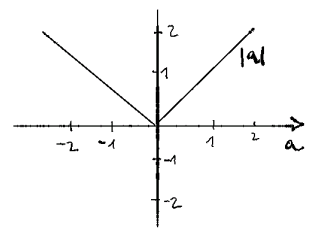
\includegraphics[width=0.4\textwidth]{betrag.png}
    \caption{Geschichte auf Linearer Zeitachse.}
    \label{fig:time_lin}
\end{figure}


\newpage
% \begin{landscape}
\begin{figure}[h!]
    \centering
    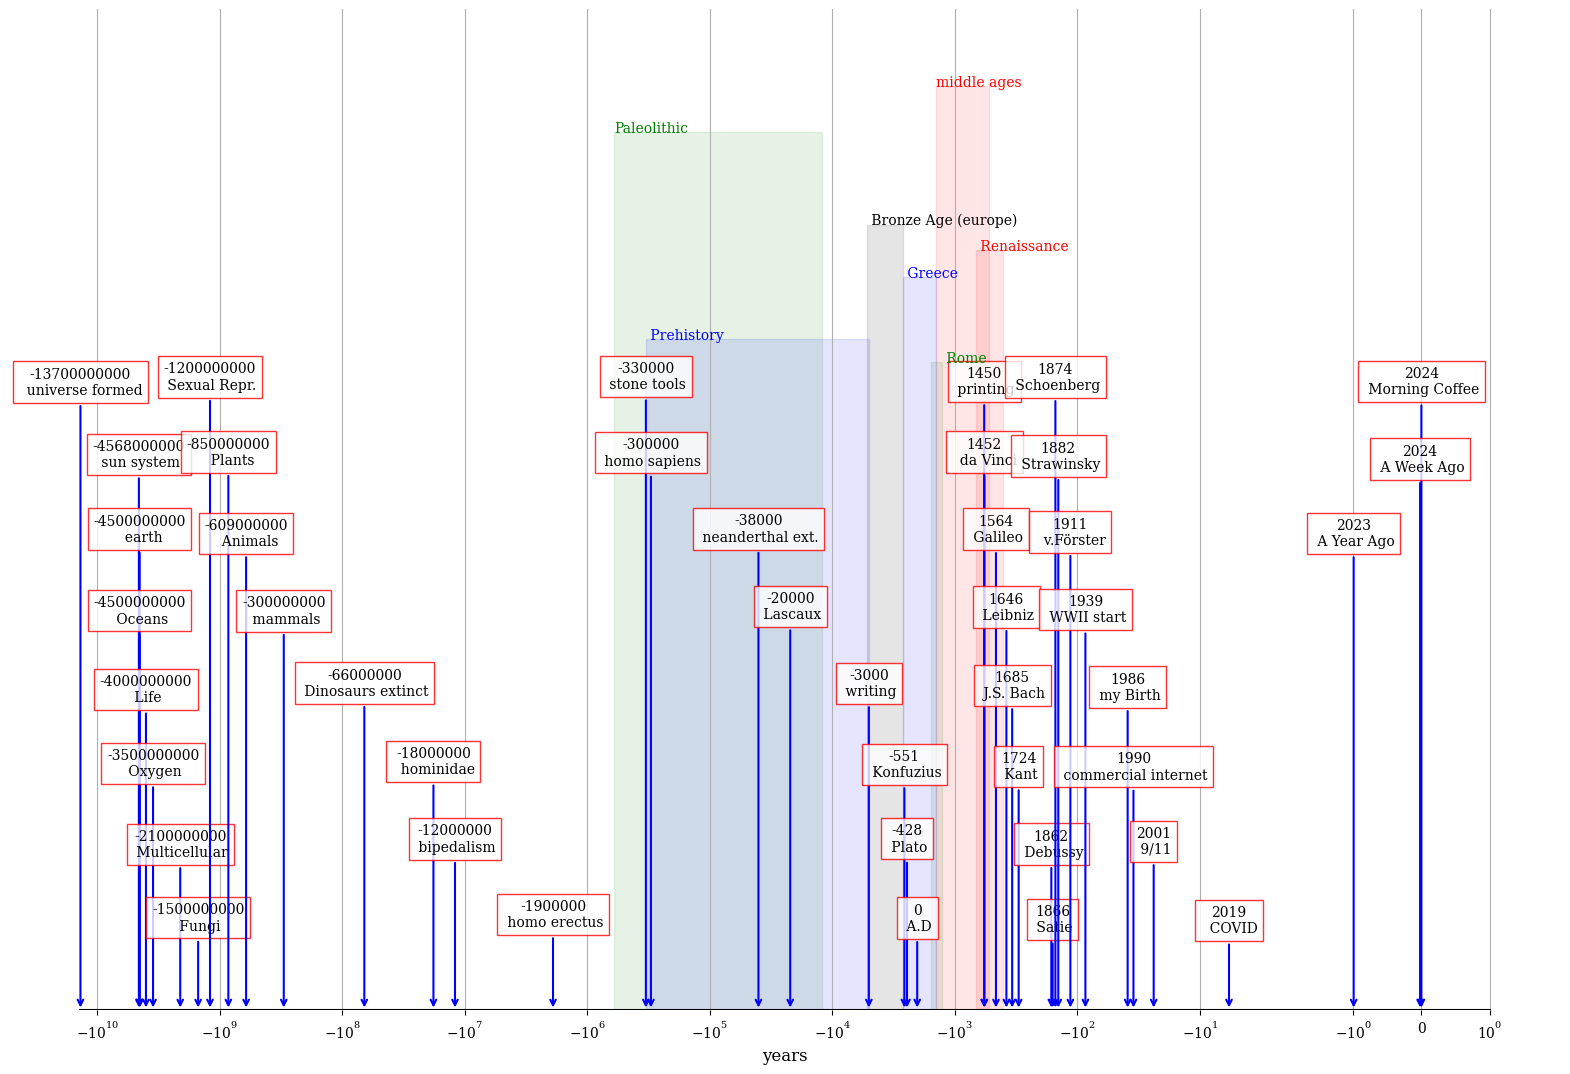
\includegraphics[height=\textwidth, angle=90]{img/time_log.png}
    \caption{Geschichte auf Logarithmischer Zeitachse.}
    \label{fig:time_log}
\end{figure}
% \end{landscape}





\section{Aufgaben und Beispiele}

\begin{enumerate}
    \item $\forall x \in \mathbb{R}, \exists y \in \mathbb{R} \text{ sodass } x + y = 0$. Was bedeutet dieser Ausdruck? Ist er wahr oder falsch?
    \item Gegeben sind die Mengen in Abb. \ref{fig:dreiMengen}. Zeichne ein Diagramm für:
    \begin{enumerate} % Use alphabetical labels for subitems
        \item $A \setminus (B \cup C)$
        \item $(A \cup B) \setminus C$
        \item $(B \cap C) \cup A$
    \end{enumerate}
    \item Zeichne einen Input/Output Plot für die Funktionen 
    \begin{enumerate} % Use alphabetical labels for subitems
        \item $f(x) = min(x, 0)$
        \item $f(x) = |x+1|-1$. Welche Bedeutung haben die beiden zahlen ($1$, $-1$ )? Wenn man sie verändern würde, was passiert mit dem Plot?
    \end{enumerate}
    \item Was gibt es zu Abb. \ref{fig:distortion_online} zu sagen?
    \item Konstruiere (mache eine Formel, formale Beschreibung) einen 'hard clipper'. Dies ist eine Verzerrung. Die Verzerrung soll keine Werte 'durchlassen' die größer als 0.9 und kleiner als -0.9 sind. Zeichne den Graphen. Für Werte zwischen -0.9 und 0.9 soll sich der Verzerrer linear verhalten. Werden hier gerade oder ungerade Harmonische Erzeugt?
    \item Berechne die 'Spannung' $T$ (eine Kraft) in einer Piano Saite. Die Grundfrequenz der Saite ist 440 Hz, sie ist aus Stahl und ca. 50 cm lang. Gegeben ist folgende Formel: $f_0 = \lambda \sqrt{\frac{T}{\rho A}}$. Hier ist $\rho$ die Dichte des Materials und $A$ der Flächendurchschnitt der Saite. Wir nehmen an sie hat einen Durchmesser $d$ von ca. 1mm. Siehe Abb. \ref{fig:string_ex}.

    \item Beweise mittels Gleichungen \ref{eq:linearity1}, \ref{eq:linearity2} oder \ref{eq:linearity3} dass $f(x)=|x|$ nicht linear ist.



\end{enumerate}

\begin{figure}[h]
    \centering
    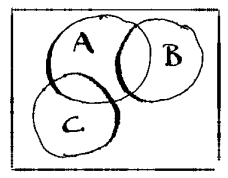
\includegraphics[width=0.3\textwidth]{img/dreiMeingen.png}
    \caption{Drei Mengen. }
    \label{fig:dreiMengen}
\end{figure}

\begin{figure}[h!]
    \centering
    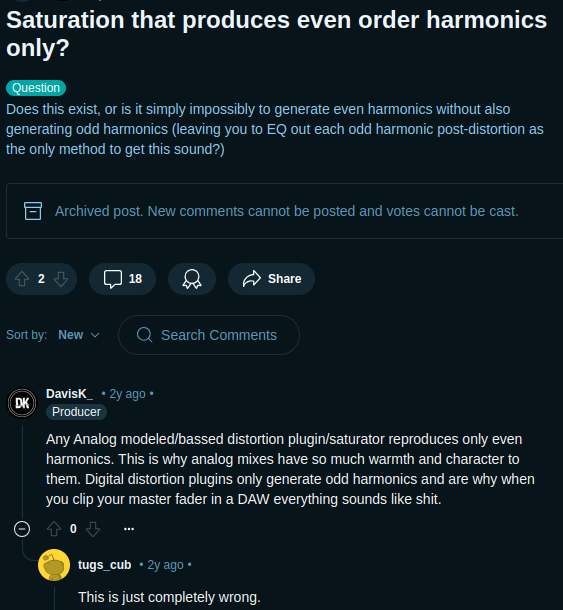
\includegraphics[ width= 0.8\textwidth]{img/reddit_distortion.png}
    \caption{Online Diskussionen über Verzerrung.}
    \label{fig:distortion_online}
\end{figure}

\begin{figure}[h!]
    \centering
    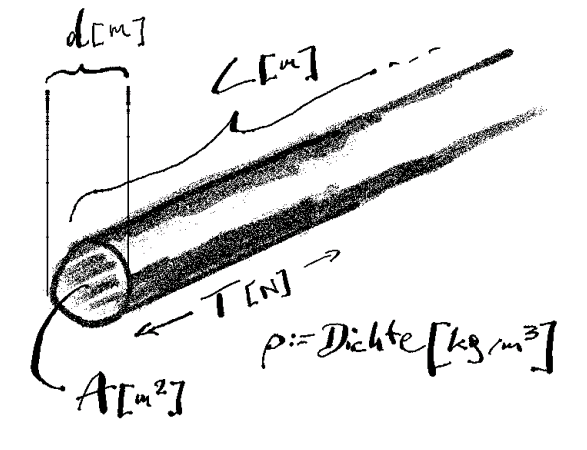
\includegraphics[ width= 0.6\textwidth]{img/saite_beispiel.png}
    \caption{Saite.}
    \label{fig:string_ex}
\end{figure}




